\documentclass[11pt, a4paper]{scrreprt}

\usepackage[T1]{fontenc}
\usepackage[english]{babel}
\usepackage{helvet}
\usepackage{graphicx}
\usepackage[dvipsnames]{xcolor}
\usepackage{mathtools}
\usepackage{bm}
\usepackage{siunitx}
\usepackage{algorithm}
\usepackage{algpseudocode}
\usepackage{subcaption}
\usepackage{appendix}
\usepackage{standalone}
\usepackage{tikz}
\usepackage[backend=biber, style=apa]{biblatex}
\usepackage{hyperref}
\usepackage[capitalise]{cleveref}

\renewcommand{\familydefault}{\sfdefault}
\usetikzlibrary{positioning, shapes.geometric, arrows, arrows.meta, positioning, calc, bending, external, backgrounds, fit, tikzmark}
\tikzexternalize[prefix=tikz_cache/]
\crefname{equation}{Eq.}{Eqs.}
\definecolor{arrowcolor}{RGB}{40, 60, 80}
\definecolor{accorange}{HTML}{D95F02}
\definecolor{accblue}{HTML}{0072B2}
\addbibresource{bibliography.bib}

\begin{document}

\begin{titlepage}
    \raggedright
    
    \vspace*{3.5cm}
    
    {\huge\bfseries Contextual Information Seeking for \\ Active Inference.\par}
    
    \vspace{3.5cm}
    
    {\Large In partial fulfillment of the requirements for the degree of \\
    Master of Science Neuroscience\par}

    \vspace{2cm}

    {\Large September 2026\par}
    
    \vspace{3.5cm}
    
    {\Large by Moritz Glawleschkoff\par}
    
    \vfill

    \noindent 
    \begin{minipage}[b]{0.45\textwidth}
        \raggedright 
        \raisebox{-0.2cm}{
\includegraphics[width=8cm]{figures/schriftzug.png}}
    \end{minipage}
    \hfill 
    \begin{minipage}[b]{0.45\textwidth}
        \raggedleft 
        
\includegraphics[height=4cm]{figures/siegel.png}\hspace*{-2cm}
    \end{minipage}

    \vspace*{-4cm}
    
\end{titlepage}
\newpage
\thispagestyle{empty} 

\vspace*{\fill} 

\noindent
{\Large 1st referee and research supervisor: Dr. Sarah Schwöbel\\[0.5cm]
2nd referee: Prof. Dr. Stefan Rotter\\[0.5cm]
3rd referee: Prof. Dr. Stefan Kiebel\par}
\chapter*{Abstract}

Humans navigate complex environments by abstracting situational details into context states, enabling efficient perception and action. The Free Energy Principle (FEP) provides a framework for understanding this behavior, positing that agents minimize expected free energy, which naturally gives rise to both goal-directed action and information-seeking (curiosity). While epistemic behavior regarding immediate environmental states has been well-studied, contextual information-seeking—where agents actively resolve uncertainty about abstract situational rules—remains underexplored. To investigate these cognitive mechanisms, this thesis develops a computational behavioral model, the Context-GFE agent, capable of actively seeking information about an abstract context state. Grounded in Active Inference and formalized using Forney-style Factor Graphs (FFG), message passing algorithms are derived to enable the unified inference of past, present, and future belief distributions. The newly proposed Context-GFE agent is evaluated against three baseline models (BFE, Context-BFE, and GFE) in a simulated T-maze environment. Results demonstrate that the Context-GFE agent successfully resolves contextual uncertainty by planning ahead to receive informative observations, balancing epistemic and pragmatic drives. Overall, this model provides a mathematically grounded and testable hypothesis for studying contextual abstraction and cognitive control, facilitating future empirical validation through Bayesian model comparison.
\tableofcontents
\chapter{Introduction}
\label{introduction}

Humans navigate complex environments by leveraging their perceptual capabilities in order to act purposefully in existential terms. Upon making an observation they must consider arbitrarily many causes in the environment. Knowing the causes of observations is important because they may pose a threat which the indiviual should counteract via actions. Having to account for a possibly indefinite number of origins of observations means a computational challenge for the human brain. Evolution has come up with a solution to this: Abstraction. Instead of having a model for each and every detail in the environment, humans are able to abstract and thus can file away functionally similar causes as singular entities. For example, when a person has learned how to do grocery shopping at a certain store, then she is also able to this at another store without relearning every detail of the new shop and how to navigate it. She posseses the abstract knowledge of grocery shopping and can apply this knowledge purposefully even if the details have changed.

Abstraction can be considered as having a context state that is "activated" during certain situations. In this way, perception is interpreted in the light of a specific context. This has been investigated in different forms: \textcite{millerandcohen2001} proposed that the prefrontal cortex maintains certain (context) patterns of activity that provide bias signals to other brain structures. In this case these patterns represent goals of the individual. With respect to vision, \textcite{raoandballard1999} discussed a hierarchy of cortical areas where higher-order areas provide (contextual) feedback connections to lower-order areas to efficiently process visual input. Moreover, the balancing between habitual- and goal-directed behavior was also proposed with respect to a context state: \textcite{schwoebel2021} developed a computational model of behavior in which an abstract context state (to be inferred) then either leads to automatic habitual behavior or starts a computationally demanding planning process in which different sequences of actions are evaluated. This model was discussed with respect to substance use disorder, which is a habitual trait that is context dependent. Concluding, the existence of abstract context states is evident both in neural wetware and in models of behavior.

As touched upon earlier, existence is the central problem every human must face. While contextual abstraction allows for tractable computation (inference) of causes (that generate observations) the mechanisms of utilizing this knowledge of hidden environmental causes remains to be addressed: According to the free energy principle (FEP) (\cite{friston2010}), individuals are equipped with a generative model that relates environmental causes with observations. Moreover, it recognizes that existence can be equated with maintaining a non-equilibrium steady state (NESS) distribution (\cite{friston2013}), i.e, the individual "wants" to remain in a state that is typical for its ecological niche and phenotype. In other words, the animal is inclined to maintain likely states that underwrites its existence. In its more general form the principle suggests that the whole individual is a generative model. Under this perspective the individual might be seen as a functional homomorphism of its ecological niche, i.e, it keeps stable (survives) because environmental influences (including observations) get "explained away" by its physiological structure. In the FEP it is then concluded that animals maintain their NESS by minimizing the variational free energy (VFE) with respect to their generative models. Moreover, VFE is a quantity that relates to the present because existence itself relates to the present. Following this, the only self consistent belief an individual can have is that it also minimizes its VFE in the future, i.e., it should perform actions that fulfill this requirement. Interestingly, when planning sequences of actions that minimize VFE in future the animal does not solely realize preferred observations that are typical for its ecological niche (e.g., most humans do not "like" the gaze of spiders because they are potentially venomous) but also shows curiousity (\cite{friston2015}), i.e., it seeks information in the environment that disambiguates hidden causes (of observations) which makes its life more predictable and therefore secure.

Following this, it is plausible that an individual not only shows curiousity with respect to immediate environmental causes but also attempts to seek information about the more abstract context that might currently be active. For example, consider a group of people who plays cards. A new player likely asks for the rules before joining. In this situation the new player wants to find out about the context "game rules" by seeking information in the environment "asking the other players". This pattern seems to be cental to human behavior.

In this thesis I attempt to develop a behavioral computational model that may account for contextual information seeking in humans. The model integrates central pillars of intelligent behavior, e.g., perception, planning, action, and inference. A central motivation for this work is the model's usage in Bayesian model comparison, i.e, it can be understood as a hypothesis about behavior that can be validated by empirical data from experiments with human participants. While this perspective makes it useful for neuroscientific and psychological research, in this work I view the behavioral model as an agent to be able to explicitly show the kind of behavior that can be explained by this model. Concretely, I develop an agent and demonstrate its contextual information seeking behavior in simulated experiments in the T-Maze envirnonment that is usually used to show this kind of behavior in discrete agents that function akin to the free energy principle (\cite{friston2015}). This last point effectively makes the agent an active inference agent (\cite{friston2010aif}).

Active inference agents are behaving entities that entail generative models that allow them to "understand" the relationships between observations, hidden environmental states (causes), and the succession of hidden states when influenced by actions. Using this model, the agent can integrate current observations, infer its likely causes in the environment, simulate how sequences of actions lead to future observations that it either likes or dislikes (with respect to its preferences), and finally select actions that it expects to yield the lowest variational free energy in the future. These behavioral "functions" can be framed as a unified inference process during which the agent infers belief distributions with respect to observations, hidden states, and actions at different timesteps (past, present, and future). When developing computational models of these mechanisms, Forney factor graphs have proven to be useful theoretical substrates that are able to capture the generative model (unrolled in time), the belief distributions, and the unified inference process as messages sent through this graph (\cite{loeliger2004,delaar2019}). While the usage of Forney graphs makes the underlying mathematical foundation of active inference agents more visually accessible they also lend some plausability as a model of brain function where computations are equivalently distributed and neural signaling might be analog to local messages sent in the factor graph (\cite{bastos2012,friston2017}). Following this, the agent to be developed in this work will be based on a Forney factor graph representation.

Specifically, I will resort to an approach presented by \textcite{senoez2021,delaar2023,delaar2025}. In this, we start with the definition of the agent's generative model (unrolled in time). Next, we view this model as its Forney factor graph representation and introduce a Bethe free energy \(F\) that relates different parts of the generative model with additional belief distributions \(q\) that exist on the edges (and nodes) in the factor graph. Following this, we introduce constraints to this free energy that relate to local marginalization constraints, but also to the information seeking mechanism among others, which leads to a corresponding Lagrangian \(L\). From this we derive stationary solutions for the belief distributions and leverage the marginalization constraints to derive local messages in the factor graph. During this derivation it also becomes obvious that these messages allow for a direct computation of the belief distributions. Effectively, I derive a message passing algorithm for the agent that implements an inference process and yields infered belief distributions as a result.

Towards the development of an active inference agent that supports contextual information seeking (named Context-GFE agent in this work), I also implement three other agents that serve as starting points for this attempt: First, I reproduce two simpler agents (BFE- and GFE agent) from ... that do not entail an abstract context state but only (normal) hidden states as part of their generative models. Both are similar but the GFE agent additionally is able to perform information seeking over its (normal) hidden state. In this work, the introduction of these two agents has three reasons: First, I can show how the integration of the information seeking mechanism in the GFE agent over the BFE agent generally works. Second, both agents can serve as baselines during the simulations to reveal the kind of behavior that is expected from an agent that performs informations seeking (GFE agent) in comparison to an agent without this ability (BFE agent). Third, the BFE agent serves as a basis towards the implementation of the Context-GFE agent. This last point requires further explanation: I expand the BFE agent by an additional context state which leads to the Context-BFE agent. As a side note: The Context-BFE agent is also inspired by the Bayesian contextual control model developed by \textcite{schwoebel2021} but lacks the balancing between habitual and goal-directed behavior. Having developed the Context-BFE agent I finally take the integration of the information seeking mechanism in the GFE agent as a blueprint to implement this mechanism in the Context-BFE agent–-–but over its context state, which eventually leads to the Context-GFE agent.

In \cref{sec:0} I give an introduction to active inference. \cref{sec:1} presents the general procedere of deriving message passing algorithms from custom Lagrangians that relate generative models with belief distributions represented by Forney factor graphs. Moreover, in \cref{sec:2} I derive the four agents (BFE, GFE, Context-BFE, and Context-GFE) and present the experimental setups in \cref{sec:3}. \cref{results} presents the results of the experiments and in \cref{discussion} I give a corresponding discussion. The thesis concludes with \cref{conclusion}.
\chapter{Methods}
\section{Inference via Message Passing}
\label{sec:1}

In this section I present a method for deriving message passing algorithms that enable inference. Inference is the mechanism that allows behavioral agents (presented in later sections) to process observations, infer unobservable environmental states, perform planning, and infer useful actions. The underlying message passing algorithm rests upon a factor graph representation of the agents' generative models where messages are sent along the edges.

To focus on the core aspects of this mechanism I give the derivations including a numerical example for a simple agent that can receive observations and infer hidden environmental causes but it cannot plan nor act.

Concretely, the simple agent is concerned with its cat (yes, the agent has a pet). He is \(90\,\%\) certain that its cat is a sweet, loving angel. Unfortunately, the agent cannot look inside the cat's brain to really find out but can only observe her behavior. Sometimes, the cat walks straight up to a full glas of water, makes eye contact with the agent and pushes the glas from the table (breaks glas). The agent believes: If the cat were a little chaos demon this is exactly the kind of behavior I expect (with \(99\,\%\) certainty). On the other hand, if she really was a sweet loving angel then she would rarely do such cruel things (maybe \(10\,\%\) chance).

The agent's model of this situation can formally be described via a (generative) model \(p(s,o)=p(o|s)p(s)\) consisting of a prior probability \(p(s)\) about hidden causal states \(s\) (is the cat an angel or a daemon?) and a likelihood distribution \(p(o|s)\) that relates the hidden states to observations \(o\) (does the cat break glas or not?) as
\begin{alignat*}{3}
     & p(s=\text{"angel"})             &  &                    &  & = 0.9  \\
     & p(s=\text{"demon"})             &  &                    &  & = 0.1  \\
     & p(o=\text{"breaks glas"}        &  & |s=\text{"demon"}) &  & = 0.99 \\
     & p(o=\text{"doesn't break glas"} &  & |s=\text{"demon"}) &  & = 0.01 \\
     & p(o=\text{"breaks glas"}        &  & |s=\text{"angel"}) &  & = 0.1  \\
     & p(o=\text{"doesn't break glas"} &  & |s=\text{"angel"}) &  & = 0.9.
\end{alignat*}
With this probabilistic model the agent can then infer the true character of its cat upon making an observation. This inference can be computed via Bayes theorem. For example when the agent observes \(o=\text{"breaks glas"}\) it can calculate the posterior probability
\begin{equation*}
    p(s|o=\text{"breaks glas"}) = \frac{p(o=\text{"breaks glas"}|s)p(s)}{\sum_s p(o=\text{"breaks glas"}|s)p(s)},
\end{equation*}
which concretely results in
\begin{alignat*}{3}
     & p(s=\text{"angel"}|o=\text{"breaks glas"})  &  & \approx 0.48  \\
     & p(s=\text{"daemon"}|o=\text{"breaks glas"}) &  & \approx 0.52,
\end{alignat*}
i.e, the agent infers that the cat's character is quite ambiguous and he is actually slightly more certain that she is a demon (\(52\,\%\)).

This inference can be formalized as a message passing algorihm on a factor graph. Towards this, I will first give the simple agent's generative model as its (Forney) factor graph representation.

\subsection{The Forney Factor Graph Representation}
A Forney factor graph (FFG) is a neat tool to represent a factorized probabilistic model where probabilistic factors (e.g., \(p(s)\)) become nodes and variables (e.g., \(s\)) become edges. The generative model of the simple agent has two variables \(s\), and \(o\) and consists of two factors \(p(s)\) and \(p(o|s)\). This leads to an FFG that equally has two edges and two nodes as shown in Fig.~\ref{fig:1}.
\begin{figure}[htbp]
    \centering

    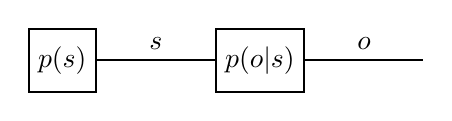
\begin{tikzpicture}[
            factor/.style={draw=black, thick, rectangle, minimum size=0.8cm, font=\normalsize},
            edge/.style={thick},
            varlabel/.style={font=\normalsize}
        ]

        % Knoten
        \node[factor] (a) {$p(s)$};
        \node[factor, right=1.5cm of a] (b) {$p(o|s)$};

        % Kanten
        \draw[edge] (a.east) -- (b.west) node[midway, above, varlabel] {$s$};
        \draw[edge] (b.east) -- ++(1.5cm, 0) node[midway, above, varlabel] {$o$};

    \end{tikzpicture}

    \caption{FFG of the model \(p(s,o)\).}
    \label{fig:1}
\end{figure}

In this work we utilize a version of an FFG that requires every edge to be terminated by a node on both ends, resulting in a (terminated) Forney factor graph. To this end, the model \(p(s,o)\) can be extended by a factor of 1 resulting in \(p(s,o)=p(s)p(o|s)\cdot1\) with the (terminated) FFG shown in Fig.~\ref{fig:2}
\begin{figure}[htbp]
    \centering

    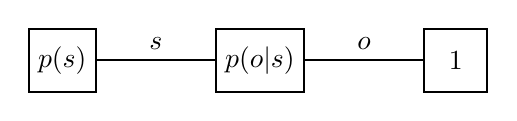
\begin{tikzpicture}[
            factor/.style={draw=black, thick, rectangle, minimum size=0.8cm, font=\normalsize},
            edge/.style={thick},
            varlabel/.style={font=\normalsize}
        ]

        % Knoten
        \node[factor] (a) {$p(s)$};
        \node[factor, right=1.5cm of a] (b) {$p(o|s)$};
        \node[factor, right=1.5cm of b] (c) {$1$};

        % Kanten
        \draw[edge] (a.east) -- (b.west) node[midway, above, varlabel] {$s$};
        \draw[edge] (b.east) -- (c.west) node[midway, above, varlabel] {$o$};

    \end{tikzpicture}

    \caption{FFG of the model \(p(s,o)\) with terminated edges.}
    \label{fig:2}
\end{figure}

To facilitate future derivations we rename node factors with functions \(f\) that have indices as unique identifiers. Following this shift, the three nodes become \(p(s)=f_a(s)\), \(p(o|s)=f_b(s,o)\), and \(1=f_c(o)\) resulting in the FFG in Fig.~\ref{fig:3}. Note that \(f_c\) has an argument \(o\) because it is connected to the edge \(o\) but always results into \(1\).
\begin{figure}[htbp]
    \centering

    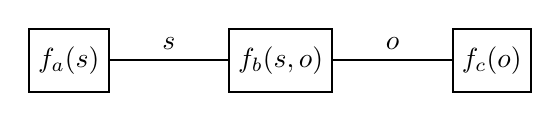
\begin{tikzpicture}[
            factor/.style={draw=black, thick, rectangle, minimum size=0.8cm, font=\normalsize},
            edge/.style={thick},
            varlabel/.style={font=\normalsize}
        ]

        % Knoten
        \node[factor] (a) {$f_a(s)$};
        \node[factor, right=1.5cm of a] (b) {$f_b(s,o)$};
        \node[factor, right=1.5cm of b] (c) {$f_c(o)$};

        % Kanten
        \draw[edge] (a.east) -- (b.west) node[midway, above, varlabel] {$s$};
        \draw[edge] (b.east) -- (c.west) node[midway, above, varlabel] {$o$};

    \end{tikzpicture}

    \caption{FFG of the model \(p(s,o)\) with renamed factors (\(f_a(s)\), \(f_b(s,o)\), \(f_c(o)\)).}
    \label{fig:3}
\end{figure}

\subsection{Belief Distributions}

In the numerical example I conditioned the generative model on a specific observation ("breaks glas") and computed the posterior distribution(s) of the remaining variables (only \(s\)). This conditioning on specific events is the "driving force" during inference that effectively "pushes" the probability mass of the remaining variables to its respective posterior forms. These form-flexible (variational) distributions exist for all variables (and factors) and effectively represent the agent's beliefs about these variables (and factors). Concretely, these belief distributions are named \(q\) and exist for all edges and nodes (for all variables and factors) in the graph (\cref{fig:4}).
\begin{figure}[htbp]
    \centering

    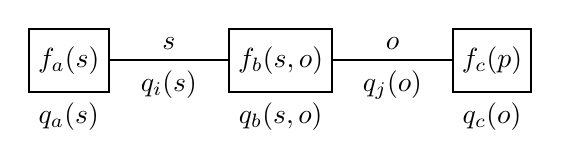
\begin{tikzpicture}[
            factor/.style={draw=black, thick, rectangle, minimum size=0.8cm, font=\normalsize},
            edge/.style={thick},
            varlabel/.style={font=\normalsize}
        ]

        % Knoten
        \node[factor, label={[varlabel]below:$q_a(s)$}] (a) {$f_a(s)$};
        \node[factor, label={[varlabel]below:$q_b(s,o)$}, right=1.5cm of a] (b) {$f_b(s,o)$};
        \node[factor, label={[varlabel]below:$q_c(o)$}, right=1.5cm of b] (c) {$f_c(p)$};

        % Kanten
        \draw[edge, ] (a.east) -- (b.west) node[midway, above, varlabel] {$s$} node[midway, below, varlabel] {$q_i(s)$};
        \draw[edge] (b.east) -- (c.west) node[midway, above, varlabel] {$o$} node[midway, below, varlabel] {$q_j(o)$};

    \end{tikzpicture}

    \caption{FFG of the model \(p(s,o)\) with belief distributions \(q\).}
    \label{fig:4}
\end{figure}
Relating to the numerical example, the conditioning of the generative model on the observation ("breaks glas") is realized by "clamping" the respective belief distribution (\(q_j(o)\)) to this event, i.e., it is set to delta distribution that has probability \(1\) for the event "breaks glas". This clamping exerts a kind of "force" on all other belief distributions and "pushes" them to their posterior forms. For example, after inference the belief \(q_i(s)\) will assume the posterior \(p(s|o=\text{"breaks glas"})\). In summary, we can now represent the agent's generative model as a factor graph and understand that it maintains belief distributions \(q\) that are form-flexible and "react" to new evidence (e.g., an observation) anywhere in the graph to form posteriors

\subsection{The (Bethe) Free Energy Functional}

As a next step towards the message passing procedere that drives inference (which forms the \(q\) distributions), it is important to realize that the metaphorical force that exists between the belief distributions (and the factors of the generative model) can exactly be defined as a variational free energy \(F[q]\). It is a functional of the belief distributions (indicated by \(q\)) and is defined as the Kullback-Leibler divergence between the joint belief distribution \(q(s,o)\) and the generative model \(p(s,o)\) with
\begin{equation}
    F[q] = D_{\mathrm{KL}}(q(s,o) \parallel p(s,o)) = \sum_{s,o} q(s,o) \log \frac{q(s,o)}{p(s,o)},
\end{equation}
where the joint belief distribution is the product of all node beliefs divided by the product of all edge beliefs, i.e., \(q(s,o)=\frac{q_a(s)q_b(s,o)q_c(o)}{q_i(s)q_j(o)}\). In this case \(F\) is equal to the Bethe free energy. Note that we assumed discrete distributions (e.g., categorical), leading to a sum instead of an integral.

For the message passing algorithm we must identify local messages that are sent on the edges of the factor graph. These local messages are driven by local free energies, which are part of the global free energy \(F\). To facilitate the derivations of these local messages, it is convenient to partition \(F\) into a sum of these local free energies. Following this, \(F\) can be rearranged to
\begin{equation}
    \begin{split}
        F[q] = & \underbrace{\sum_s q_a(s) \log \frac{q_a(s)}{f_a(s)} + \sum_{s,o} q_b(s,o) \log \frac{q_b(s,o)}{f_b(s,o)} + \sum_o q_c(o) \log \frac{q_c(o)}{f_c(o)}}_{\text{Local Free Energy Terms}} \\
               & + \underbrace{\sum_s q_i(s) \log \frac{1}{q_i(s)} + \sum_o q_j(o) \log \frac{1}{q_j(o)}}_{\text{Correcting Entropy Terms}}.
    \end{split}
\end{equation}
This yields three node-local free energy terms that measure the Kullback-Leibler divergence between the local belief distribution \(q\) and the local factor \(f\). Importantly, these local free energies contain entropy terms that correspond to the edges' entropies they are connected to. As an example consider the first local free energy term \(\sum_s q_a(s) \log \frac{q_a(s)}{f_a(s)}\) which can be decomposed into \(- (-\sum_s q_a(s) \log q_a(s)) - \sum_s q_a(s) \log f_a(s)\). The term \(- (-\sum_s q_a(s) \log q_a(s))\) is the entropy of edge \(i\), i.e., it is equivalent to \(- (-\sum_s q_i(s) \log q_i(s))\). Similarly node \(b\) also contains this entropy of edge \(i\) as part of \(- (-\sum_{s,o} q_b(s,o) \log q_b(s,o))\). Consequently, having two nodes for every edge results into overcounting of edge entropies, i.e., it is subtracted twice. To correct for this, one entropy term is added for each edge in \(F\), e.g., \(\sum_s q_i(s) \log \frac{1}{q_i(s)}\). This corrective measure is not a deliberative choice but a natural consequence of defining belief distributions over edges and nodes in the graph. This circumstance makes the variational free energy \(F\) equal to the Bethe free energy.

\subsection{The Lagrangian of the Free Energy}

Now, that I have defined the "force" that couples the belief distributions with the factors of the generative model, i.e., \(F\), and how it can be decomposed to a sum of local terms, it next becomes necessary to understand that the belief distributions \(q\) are freely optimizable functions that do not automatically satisfy the requirements of probability distributions. Concretely, first they must meet the normalization constraints

\noindent
\begin{minipage}[t]{0.5\textwidth}
    \setlength{\abovedisplayskip}{0pt}
    \setlength{\belowdisplayskip}{0pt}
    \begin{align}
        \sum_s q_a(s)       & \overset{!}{=} 1 \\[0.1em]
        \sum_{s,o} q_b(s,o) & \overset{!}{=} 1 \\
        \sum_o q_c(o)       & \overset{!}{=} 1
    \end{align}
\end{minipage}\hfill
\begin{minipage}[t]{0.5\textwidth}
    \setlength{\abovedisplayskip}{0pt}
    \setlength{\belowdisplayskip}{0pt}
    \begin{align}
        \sum_s q_i(s) & \overset{!}{=} 1  \\
        \sum_o q_j(o) & \overset{!}{=} 1,
    \end{align}
\end{minipage}
and second they must meet marginalization constraints with respect to neighboring belief distributions in the factor graph with

\noindent
\begin{minipage}[t]{0.5\textwidth}
    \setlength{\abovedisplayskip}{0pt}
    \setlength{\belowdisplayskip}{0pt}
    \begin{align}
        q_i(s) & \overset{!}{=} q_a(s)          \\[0.8em]
        q_i(s) & \overset{!}{=} \sum_y q_b(s,o)
    \end{align}
\end{minipage}\hfill
\begin{minipage}[t]{0.5\textwidth}
    \setlength{\abovedisplayskip}{0pt}
    \setlength{\belowdisplayskip}{0pt}
    \begin{align}
        q_j(o) & \overset{!}{=} \sum_x q_b(s,o) \\
        q_j(o) & \overset{!}{=} q_c(o).
    \end{align}
\end{minipage}

These constraints are then added to \(F\) and lead to the Lagrangian
\begin{equation}
    \begin{split}
        L = F & + \sum_s \lambda_{ia}(s) (q_i(s) - q_a(s)) + \sum_s \lambda_{ib}(s) (q_i(s) - \sum_y q_b(s,o)) \\
              & + \sum_o \lambda_{jb}(o) (q_j(o) - \sum_s q_b(s,o)) - \sum_o \lambda_{jc}(o) (q_j(o) - q_c(o)) \\
              & + \psi_a (\sum_s q_a(s) - 1) + \psi_b (\sum_{s,o} q_b(s,o) - 1) + \psi_c (\sum_o q_c(o) - 1)   \\
              & + \psi_i (\sum_s q_i(s) - 1) + \psi_j (\sum_o q_j(o) - 1),
    \end{split}
    \label{eq:36}
\end{equation}
where \(\lambda\) und \(\psi\) are Lagrange multipliers that enforce marginalization and normalization respectively.

\subsection{Messages and Belief Updates}

Having defined the Lagrangian of the factor graph it is now possible to derive the messages that are necessary for the final belief updates. Recall, that the message passing algorithm aims at finding belief distributions \(q\) by minimizing \(F\) (which is part of \(L\)), i.e. the beliefs "relax" to their solutions driven by the metaphorical force \(F\). This "relaxation" process is realized by the message passing in the graph. Following this, \(L\) is partially differentiated with respect to each belief (variational) distribution \(q\), then variational derivatives are set to \(0\), and solved for \(q^*\):
\begin{alignat}{3}
     & \frac{\delta L}{\delta q_a(s)} &  & = \log q_a(s) + 1 - \log f_a(s) - \lambda_{ia}(s) + \psi_a             & \overset{!}{=} 0 \\
     &                                &  & \Rightarrow q_a^*(s) = f_a(s) \exp(\lambda_{ia}(s)) \exp(-\psi_a - 1). & \label{eq:6}
\end{alignat}
By a similar argument it follows that
\begin{alignat}{3}
     & \Rightarrow q_b^*(s,o) &  & = f_b(s,o) \exp(\lambda_{ib}(s)) \exp(\lambda_{jb}(o)) \exp(-\psi_b - 1)                & \label{eq:7} \\
     & \Rightarrow q_c^*(o)   &  & = f_c(o) \exp(\lambda_{jc}(o)) \exp(-\psi_c - 1)                           \label{eq:8}                \\
     & \Rightarrow q_i^*(s)   &  & = \exp(\lambda_{ia}(s)) \exp(\lambda_{ib}(s)) \exp(\psi_i - 1)             \label{eq:9}                \\
     & \Rightarrow q_j^*(o)   &  & = \exp(\lambda_{jb}(o)) \exp(\lambda_{jc}(o)) \exp(\psi_j - 1).\label{eq:10}
\end{alignat}
Second, we partially solve the system of equations (\cref{eq:6,eq:7,eq:8,eq:9,eq:10}) with respect to the normalization constraints with
\begin{alignat}{2}
     & \sum_s q_a^*(s)                                       &  & \overset{!}{=} 1                                                             \\
     & \sum_s f_a(s) \exp(\lambda_{ia}(s)) \exp(-\psi_a - 1) &  & = 1                                                                          \\
     & \exp(-\psi_a - 1) \sum_x f_a(s) \exp(\lambda_{ia}(s)) &  & = 1                                                                          \\
     & \exp(-\psi_a - 1)                                     &  & = \frac{1}{\sum_s f_a(s) \exp(\lambda_{ia}(s))}                              \\
     & \Rightarrow q_a^*(s)                                  &  & = f_a(s) \exp(\lambda_{ia}(s)) \frac{1}{\sum_s f_a(s) \exp(\lambda_{ia}(s))} \\
     & \Rightarrow q_a^*(s)                                  &  & \propto f_a(s) \exp(\lambda_{ia}(s)). \label{eq:1}
\end{alignat}
The term \(\exp(-\psi_a - 1)\) effectively becomes the normalization constant for \(q_a^*(s)\). Instead of doing this derivation repeatedly in subsequent sections, I will directly use the proportional sign \(\propto\) when defining belief distributions. More generally, in some cases I will also use "\(\propto\)" even if the relation allows for the stricter "\(=\)" sign.
Analogously we obtain
\begin{alignat}{2}
     & \Rightarrow q_b^*(s,o) &  & \propto f_b(s,o) \exp(\lambda_{ib}(s)) \exp(\lambda_{jb}(o)) \label{eq:2} \\
     & \Rightarrow q_c^*(o)   &  & \propto f_c(o) \exp(\lambda_{jc}(o))                         \label{eq:3} \\
     & \Rightarrow q_i^*(s)   &  & \propto \exp(\lambda_{ia}(s)) \exp(\lambda_{ib}(s))          \label{eq:4} \\
     & \Rightarrow q_j^*(o)   &  & \propto \exp(\lambda_{jb}(o)) \exp(\lambda_{jc}(o)).\label{eq:5}
\end{alignat}
Third, we solve the remaining system of equations (\cref{eq:1,eq:2,eq:3,eq:4,eq:5}) with respect to the marginalization constraints with
\begin{alignat}{2}
     & q_a^*(s)                          &  & \overset{!}{=} q_i(s)                               \\
     & f_a(s) \exp(\lambda_{ia}(s))      &  & \propto \exp(\lambda_{ia}(s)) \exp(\lambda_{ib}(s)) \\
     & \Rightarrow \exp(\lambda_{ib}(s)) &  & \propto f_a(s). \label{eq:26}
\end{alignat}
Similarly, it can be shown that
\begin{alignat}{2}
     & \Rightarrow \exp(\lambda_{ia}(s)) &  & \propto \sum_o f_b(s,o) \exp(\lambda_{jb}(o)) \label{eq:27}    \\
     & \Rightarrow \exp(\lambda_{jc}(o)) &  & \propto \sum_s f_b(s,o) \exp(\lambda_{ib}(s))    \label{eq:28} \\
     & \Rightarrow \exp(\lambda_{jb}(o)) &  & \propto f_c(o). \label{eq:29}
\end{alignat}
Crucially, the derivations do not only yield the messages but also how they can be used to finally compute the belief distributions \(q\). Concretely, the final beliefs are given in \cref{eq:2,eq:3,eq:4,eq:5} and thus depend on the messages \(\exp(\lambda_{ib}(s))\), \(\exp(\lambda_{jb}(o))\), \(\exp(\lambda_{jc}(o))\), and \(\exp(\lambda_{ia}(s))\). Moreover, the definitions of these four messages are given in \cref{eq:26,eq:27,eq:28,eq:29}.

\subsection{Messages in the Factor Graph}
Having derived the four messages above, we can now view them inside the factor graph.
Their names give a clear interpretation of their position and direction of information flow in the graph. For example, the message \(\exp(\lambda_{ia}(s))\) has indices \(i\) and \(a\), meaning that its location in the FFG is on the edge \(i\) and points towards node \(a\). The resulting graph with all messages is given in Fig.~\ref{fig:6}.
\begin{figure}[htbp]
    \centering

    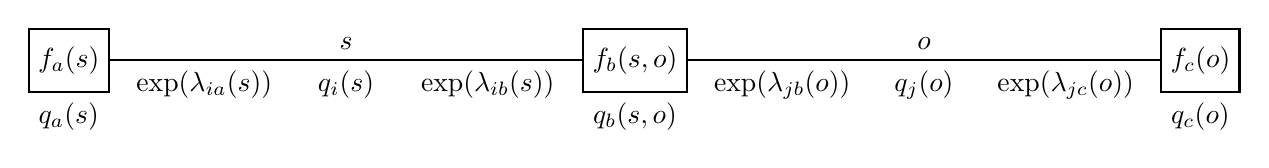
\begin{tikzpicture}[
            factor/.style={draw=black, thick, rectangle, minimum size=0.8cm, font=\normalsize},
            edge/.style={thick},
            varlabel/.style={font=\normalsize},
            greycircle/.style={draw=black, thick, circle, fill=gray!30, minimum size=0.5cm, font=\normalsize}
        ]

        % Knoten
        \node[factor, label={[varlabel]below:$q_a(s)$}] (a) {$f_a(s)$};
        \node[factor, label={[varlabel]below:$q_b(s,o)$}, right=6cm of a] (b) {$f_b(s,o)$};
        \node[factor, label={[varlabel]below:$q_c(o)$}, right=6cm of b] (c) {$f_c(o)$};

        % Kanten
        \draw[edge] (a.east) -- (b.west) node[midway, above, varlabel] {$s$} node[midway, below, varlabel] {$q_i(s)$} node[pos=0.2, below, varlabel] {$\exp(\lambda_{ia}(s))$}  node[pos=0.8, below, varlabel] {$\exp(\lambda_{ib}(s))$};
        \draw[edge] (b.east) -- (c.west) node[midway, above, varlabel] {$o$} node[midway, below, varlabel] {$q_j(o)$} node[pos=0.2, below, varlabel] {$\exp(\lambda_{jb}(o))$}  node[pos=0.8, below, varlabel] {$\exp(\lambda_{jc}(o))$};

    \end{tikzpicture}

    \caption{FFG of the model \(p(s,o)\) with messages.}
    \label{fig:6}
\end{figure}

Using the full message names renders the FFG visually overloaded.
Instead we use abbreviations (\(\textcolor{black}{\bm{\overleftarrow{\mu}}},\textcolor{black}{\bm{\overrightarrow{\mu}}}\)) with arrows clearly indicating the direction of information flow with \(\textcolor{black}{\bm{\overleftarrow{\mu}(}s\bm{)}} = \exp(\lambda_{ia}(s))\), \(\textcolor{black}{\bm{\overrightarrow{\mu}(}s\bm{)}} = \exp(\lambda_{ib}(s))\), \(\textcolor{black}{\bm{\overleftarrow{\mu}(}o\bm{)}} = \exp(\lambda_{jb}(o))\), and \(\textcolor{black}{\bm{\overrightarrow{\mu}(}o\bm{)}} = \exp(\lambda_{jc}(o))\).
The resulting FFG is given in Fig.~\ref{fig:7}.
\begin{figure}[htbp]
    \centering

    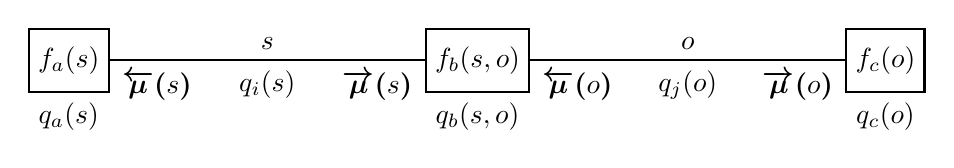
\begin{tikzpicture}[
            factor/.style={draw=black, thick, rectangle, minimum size=0.8cm, font=\normalsize},
            edge/.style={thick},
            varlabel/.style={font=\normalsize},
            greycircle/.style={draw=black, thick, circle, fill=gray!30, minimum size=0.5cm, font=\normalsize}
        ]

        % Knoten
        \node[factor, label={[varlabel]below:$q_a(s)$}] (a) {$f_a(s)$};
        \node[factor, label={[varlabel]below:$q_b(s,o)$}, right=4cm of a] (b) {$f_b(s,o)$};
        \node[factor, label={[varlabel]below:$q_c(o)$}, right=4cm of b] (c) {$f_c(o)$};

        % Kanten
        \draw[edge] (a.east) -- (b.west) node[midway, above, varlabel] {$s$} node[midway, below, varlabel] {$q_i(s)$} node[pos=0.15, below, varlabel] {$\textcolor{black}{\bm{\overleftarrow{\mu}(}s\bm{)}}$}  node[pos=0.85, below, varlabel] {$\textcolor{black}{\bm{\overrightarrow{\mu}(}s\bm{)}}$};
        \draw[edge] (b.east) -- (c.west) node[midway, above, varlabel] {$o$} node[midway, below, varlabel] {$q_j(o)$} node[pos=0.15, below, varlabel] {$\textcolor{black}{\bm{\overleftarrow{\mu}(}o\bm{)}}$}  node[pos=0.85, below, varlabel] {$\textcolor{black}{\bm{\overrightarrow{\mu}(}o\bm{)}}$};

    \end{tikzpicture}

    \caption{FFG of the model \(p(s,o)\) with \(\bm{\mu}\) messages.}
    \label{fig:7}
\end{figure}
In principle, the message passing algorithm is now complete and messages can be computed to finally determine the belief distributions. Still missing is the explicit modeling of the observation in the factor graph. Without an observation, inference has no basis for computing beliefs that relate to posteriors. Next I show the integration of an observation in the factor graph and how that locally leads to alternative messages.

\subsection{Observation (Delta) Constraints}

Having a concrete observation \(\hat o\) for a variable \(o\) renders its corresponding (edge) belief distribution \(q_j(o)\) a delta distribution. This effectively assigns all probability mass to this single observation while other events have probability \(0\). In this work, distributions are discrete such that delta distributions are given as Kronecker deltas that evaluate to \(1\) for the respective observation event. Relating to the cat example, the delta distribution is given as \(\delta_{o,\hat o}\) with \(\hat o = \text{"breaks glas"}\), i.e., only the event "breaks glas" evaluates to \(1\), and thus defines the edge's belief distribution as \(q_j(o) = \delta_{o,\hat o}\). This delta constraint is visualized in the factor graph (\cref{fig:29}) by a gray bead at the respective edge.
\begin{figure}[htbp]
    \centering

    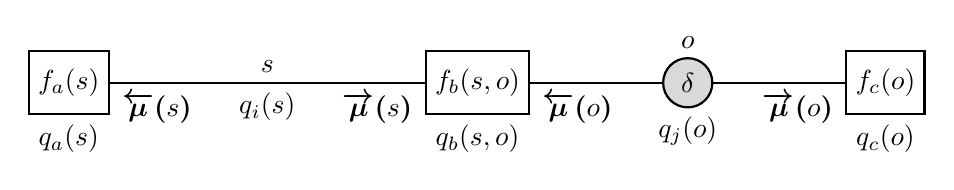
\begin{tikzpicture}[
            factor/.style={draw=black, thick, rectangle, minimum size=0.8cm, font=\normalsize},
            edge/.style={thick},
            varlabel/.style={font=\normalsize},
            greycircle/.style={draw=black, thick, circle, fill=gray!30, minimum size=0.5cm, font=\normalsize}
        ]

        % Knoten
        \node[factor, label={[varlabel]below:$q_a(s)$}] (a) {$f_a(s)$};
        \node[factor, label={[varlabel]below:$q_b(s,o)$}, right=4cm of a] (b) {$f_b(s,o)$};
        \node[factor, label={[varlabel]below:$q_c(o)$}, right=4cm of b] (c) {$f_c(o)$};

        % Kanten
        \draw[edge] (a.east) -- (b.west) node[midway, above, varlabel] {$s$} node[midway, below, varlabel] {$q_i(s)$} node[pos=0.15, below, varlabel] {$\textcolor{black}{\bm{\overleftarrow{\mu}(}s\bm{)}}$}  node[pos=0.85, below, varlabel] {$\textcolor{black}{\bm{\overrightarrow{\mu}(}s\bm{)}}$};
        \draw[edge] (b.east) -- (c.west) node[midway, greycircle] {$\delta$} node[midway, above=0.3, varlabel] {$o$} node[midway, below=0.3, varlabel] {$q_j(o)$} node[pos=0.15, below, varlabel] {$\textcolor{black}{\bm{\overleftarrow{\mu}(}o\bm{)}}$}  node[pos=0.85, below, varlabel] {$\textcolor{black}{\bm{\overrightarrow{\mu}(}o\bm{)}}$};

    \end{tikzpicture}

    \caption{FFG of the model \(p(s,o)\) with delta constraint.}
    \label{fig:29}
\end{figure}
Importantly, introducing the constraint \(q_j(o) = \delta_{o,\hat o}\) leads to alternative messages \(\textcolor{black}{\bm{\overleftarrow{\mu}(}o\bm{)}}\) and \(\textcolor{black}{\bm{\overrightarrow{\mu}(}o\bm{)}}\). These messages are derived in the following.

Starting point for this derivation are the local stationary solutions from \cref{eq:1,eq:2,eq:3,eq:4,eq:5}. During the following resolution of marginalization constraints that depend on \(q_j(o)\) (i.e., \cref{eq:28,eq:29} in prior derivations) the belief \(q_j(o)\) is substituted by \(\delta_{o,\hat o}\), which leads to:
\begin{alignat}{2}
     & \sum_s q_b^*(s,o)                                                                           &  & \overset{!}{=} q_j^*(o)                                                               \\
     & \sum_s f_b(s,o) \exp(\lambda_{ib}(s)) \exp(\lambda_{jb}(o))                                 &  & \propto \delta_{o,\hat o}                                                             \\
     & \exp(\lambda_{jb}(o)) \sum_s f_b(s,o) \exp(\lambda_{ib}(s))                                 &  & \propto \delta_{o,\hat o}                                                             \\
     & \exp(\lambda_{jb}(o))                                                                       &  & \propto \frac{\delta_{o,\hat o}}{\sum_s f_b(s,o) \exp(\lambda_{ib}(s))} \label{eq:23} \\
     & \Rightarrow \exp(\lambda_{jb}(o))              \propto \delta_{o,\hat o}                                                                                                               \\
     & \Rightarrow \textcolor{black}{\bm{\overleftarrow{\mu}(}o\bm{)}}  \propto \delta_{o,\hat o}.
\end{alignat}
Note that \(\frac{\delta_{o,\hat o}}{\sum_s f_b(s,o) \exp(\lambda_{ib}(s))}\) in \cref{eq:23} evaluates to \(\delta_{o,\hat o}\). To understand this, consider the following two cases. First, if \(o \neq \hat o\) then both \(\frac{\delta_{o,\hat o}}{\sum_s f_b(s,o) \exp(\lambda_{ib}(s))}\) and \(\delta_{o,\hat o}\) yield 0 as the result. Second, if \(o = \hat o\) then \(\delta_{o,\hat o}\) will result into 1 and \(\frac{\delta_{o,\hat o}}{\sum_s f_b(s,o) \exp(\lambda_{ib}(s))}\) will result into some positive number (not 0). For the the latter, normalization ensures that this arbitrary number will be 1 because all other outcomes already have probability 0 as outlined in the first case.

Similarly, using the constraint \(q_c^*(o) \overset{!}{=} q_j^*(o)\) we obtain
\begin{alignat}{2}
     & \Rightarrow \textcolor{black}{\bm{\overrightarrow{\mu}(}o\bm{)}}  \propto \delta_{o,\hat o}.
\end{alignat}

Having derived the messages \(\textcolor{black}{\bm{\overleftarrow{\mu}(}o\bm{)}}\) and \(\textcolor{black}{\bm{\overrightarrow{\mu}(}o\bm{)}}\) that result from the observation \(\hat o\) we can now show how this message passing algorithm achieves the inference from the cat example. The algorithm is formally given in the following section.

\subsection{Message Passing Algorithm}

As outlined before, the algorithm consists of first computing all messages and second the edges' belief distributions and is given in \cref{alg:1}.
\begin{algorithm}[htbp]
    \caption{Message Passing Algorithm of the Simple Agent}
    \label{alg:1}
    \begin{algorithmic}[1]
        \State $\textcolor{black}{\bm{\overleftarrow{\mu}(}o\bm{)}}$,\quad$\textcolor{black}{\bm{\overrightarrow{\mu}(}o\bm{)}}$,\quad$\textcolor{black}{\bm{\overrightarrow{\mu}(}s\bm{)}}$
        \State $\textcolor{black}{\bm{\overleftarrow{\mu}(}s\bm{)}}$
        \State $q_i(s)$,\quad$q_j(o)$
    \end{algorithmic}
\end{algorithm}
Note that some messages depend on the result of other messages which leads to a certain order of execution, e.g., \(\textcolor{black}{\bm{\overleftarrow{\mu}(}s\bm{)}} \propto \sum_o f_b(s,o) \textcolor{black}{\bm{\overleftarrow{\mu}(}o\bm{)}}\) depends on \(\textcolor{black}{\bm{\overleftarrow{\mu}(}o\bm{)}}\).

In the following I present the algorithm's execution using the numerical cat example.
First, the messages \(\textcolor{black}{\bm{\overleftarrow{\mu}(}o\bm{)}}\), \(\textcolor{black}{\bm{\overrightarrow{\mu}(}o\bm{)}}\), and \(\textcolor{black}{\bm{\overrightarrow{\mu}(}s\bm{)}}\) are evaluated (there is no order between the three messages because they do not depend on each other):
\begin{alignat}{2}
     & \Rightarrow \textcolor{black}{\bm{\overleftarrow{\mu}(}o\bm{)}}  &  & \propto \delta_{o,\hat o}                     \\
     & \Rightarrow \textcolor{black}{\bm{\overrightarrow{\mu}(}o\bm{)}} &  & \propto \delta_{o,\hat o}                     \\
     & \Rightarrow \textcolor{black}{\bm{\overrightarrow{\mu}(}s\bm{)}} &  & = \exp(\lambda_{ib}(s)) \propto f_a(s) = p(s)
\end{alignat}
with \(\hat o = \text{"breaks glas"}\).

Second, \(\textcolor{black}{\bm{\overleftarrow{\mu}(}s\bm{)}}\) is evaluated:
\begin{alignat}{2}
     & \Rightarrow \textcolor{black}{\bm{\overleftarrow{\mu}(}s\bm{)}} &  & \propto \sum_o f_b(s,o) \textcolor{black}{\bm{\overleftarrow{\mu}(}o\bm{)}} = \sum_o p(o|s) \delta_{o,\hat o} = p(\hat o|s)
\end{alignat}

Third, the edges' belief distributions are computed:
\begin{alignat}{2}
     & \Rightarrow q_i(s) &  & \propto \textcolor{black}{\bm{\overleftarrow{\mu}(}s\bm{)}} \textcolor{black}{\bm{\overrightarrow{\mu}(}s\bm{)}} = p(\hat o|s) p(s)                                        \\
     & \Rightarrow q_j(o) &  & \propto \textcolor{black}{\bm{\overleftarrow{\mu}(}o\bm{)}} \textcolor{black}{\bm{\overrightarrow{\mu}(}o\bm{)}} = \delta_{o,\hat o} \delta_{o,\hat o} = \delta_{o,\hat o}
\end{alignat}
In principle, the evaluation of \(q_j(o)\) is unnecessary because it will trivially yield the start condition (delta constraint).
Finally, we can insert the probabilities from the cat example:
\begin{alignat}{2}
    q_i(s=\text{"angel"}) & \propto p(o=\text{"breaks glas"}|s=\text{"angel"}) p(s=\text{"angel"}) = 0.1 \cdot 0.9 = 0.09   \\
    q_i(s=\text{"demon"}) & \propto p(o=\text{"breaks glas"}|s=\text{"demon"}) p(s=\text{"demon"}) = 0.99 \cdot 0.1 = 0.099
\end{alignat}
After normalization, the agent's belief \(q_i(s)\) yields:
\begin{alignat}{2}
    q_i(s=\text{"angel"}) & = \frac{0.09}{0.09+0.099} \approx 0.48  \\
    q_i(s=\text{"demon"}) & = \frac{0.099}{0.09+0.099} \approx 0.52
\end{alignat}
Furthermore, the observation belief \(q_j(o)\) trivially results into
\begin{alignat}{2}
    q_j(o=\text{"breaks glas"})        & = 1  \\
    q_j(o=\text{"doesn't break glas"}) & = 0.
\end{alignat}
because it is constrained by a real observation.

In conclusion, the message passing algorithm achieves Bayesian inference and the resulting belief distribution \(q_i(s)\) is equal to the posterior \(p(s|o=\text{"breaks glas"})\) that has been analytically shown before. Furthermore, the algorithm that results from the Bethe free energy as defined in this section is also known as the sum-product algorithm or belief propagation.


\section{Agents}

In this section I present the four agents that are developed in this work. First, I detail what agents entail.

\subsubsection{The Perception-Action Loop}

In general, agents are entities that are in constant exchange with an external environment. They receive observations from and act upon the environment. In this work observations and actions occur at discrete timesteps and are signified via the variables \(o_t\) and \(a_t\) respectively at the current timestep \(t\) (\cref{fig:23}).
\begin{figure}[htbp]
    \centering
    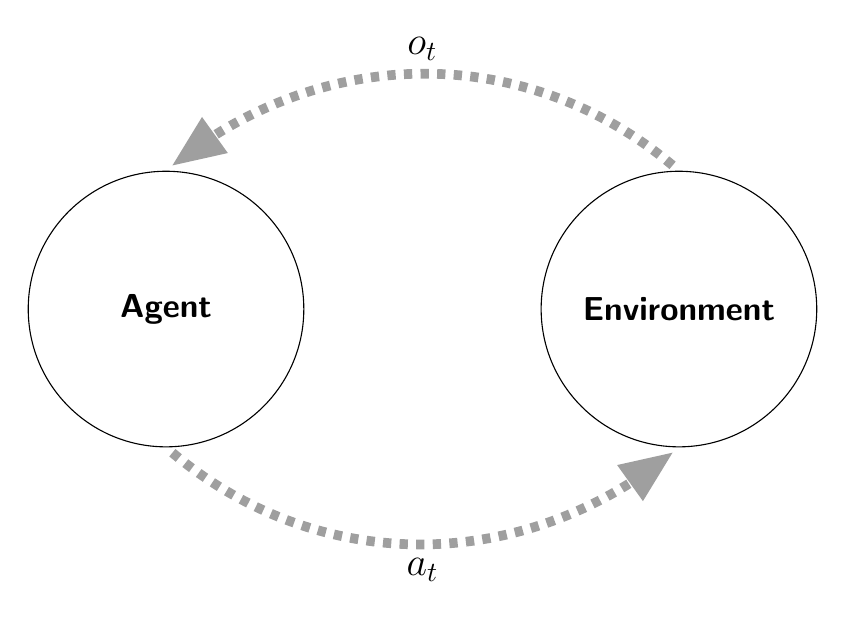
\begin{tikzpicture}[
            kreis/.style={
                    draw,
                    circle,
                    minimum size=3.5cm,
                    fill=white,
                    text centered,
                    font=\large\bfseries
                },
            pfeil/.style={
                    draw,
                    ->,
                    >={triangle 45},
                    dashed,
                    line width=3.5,
                    color=darkgray!50,
                    shorten >=3pt,
                    shorten <=3pt
                },
            label/.style={
                    midway,
                    font=\Large,
                    color=black,
                    text depth=0.5ex
                }
        ]

        \node[kreis] (agent) {Agent};
        \node[kreis, right=3cm of agent] (env) {Environment};

        \draw[pfeil] (env.north) to[bend right=40] node[label, above] {$o_t$} (agent.north);
        \draw[pfeil] (agent.south) to[bend right=40] node[label, below] {$a_t$} (env.south);

    \end{tikzpicture}
    \caption{Perception-Action Loop between the agent and the environment. The environment sends observations \(o_t\) to the agent. Vice versa, the agent sends actions \(a_t\) to the environment. The current timestep is \(t\).}
    \label{fig:23}
\end{figure}
The environment generates observations in possibly arbitrary ways but the agent is assumed to have certain mechanisms that process these observations and trigger actions. Specifically, agents are assumed to have a preference for certain observations that underwrite their ecological niche in the environment. Moreover, they are equipped with the means to understand (simulate) the chain of causality from hidden environmental causes to its sensors, i.e., they have of model how the state of the environment leads to certain observations. Even more, they also have a model of the causal chain of these unobservable (hidden) environmental states through time and how they can be influenced via actions. In total, this allows them to plan a sequence of actions that leads to preferred observations. Additionally, it allows them to keep past observations as a memory and enables them to retrospectively draw conclusions about past events in the light of new observations from the present.

\subsubsection{The Generative Model}

This mechanism rests upon a generative model that probabilistically relates observations, actions, and the (discrete) succession of hidden states. Formally, it is given by a likelihood \(p(o|s)\) that states how observations \(o\) are generated by hidden states \(s\) and by a transition model \(p(s_{t+1}|s_t,a_t)\) that defines how hidden states \(s\) change from timestep \(t\) to \(t+1\) given an action \(a_t\). Actions possess an action prior \(p(a)\) and preferences for observations are encoded by the goal prior \(\tilde{p}(o)\) that assigns higher probabilities to preferred observations.

\subsubsection{The Temporal Generative Model (POMDP)}

The four distributions (likelihood, transition model, action prior, and goal prior) are building blocks for a temporal rollout (from timestep \(0\) to \(T\)), which formally leads to a Partially Observable Markov Decision Process (POMDP). In later simulations there will be three timesteps, i.e., \(T=2\), and hidden states at \(t=0\) are initially distributed with \(p(s_0)\). The resulting POMDP is given by
\begin{equation}
    \begin{split}
        p(o_0, o_1, o_2, s_0, s_1, s_2, a_0, a_1) = \; & \tilde{p}(o_0) p(o_0|s_0) p(s_0)                \\
                                                       & \tilde{p}(o_1) p(o_1|s_1) p(s_1|s_0,a_0) p(a_0) \\
                                                       & \tilde{p}(o_2) p(o_2|s_2) p(s_2|s_1,a_1) p(a_1)
        \label{eq:15}
    \end{split}
\end{equation}
and has a factor graph representation (\cref{fig:8}) (including the variables' belief distributions \(q\) on the edges). Note, that in the POMDP (\cref{eq:15}) some variables occur in more than two factors (e.g., \(s_0\) in \(p(s_0)\), \(p(o_0|s_0)\) and \(p(s_1|s_0,a_0)\)). When representing the POMDP as a factor graph a special situation arises in which these variables (modeled by edges) should be connected to more than two factor nodes. Crucially, factor graphs are allowed to have exactly two nodes for each edge which requires an artificial duplication of variables to make them available to more than two factor nodes (e.g., \(s_0\) is duplicated to \(s^{\scriptscriptstyle I}_0\) and \(s^{\scriptscriptstyle II}_0\)). Duplicated variables are forced to be equivalent via the special equality node (indicated by the \(=\) sign) they are all connected to. Importantly, this situation is only a formal requirement of factor graphs and has no consequences for the results of inference processes presented in following sections.

\begin{figure}[htbp]
    \centering

    \resizebox{1.0\textwidth}{!}{%
        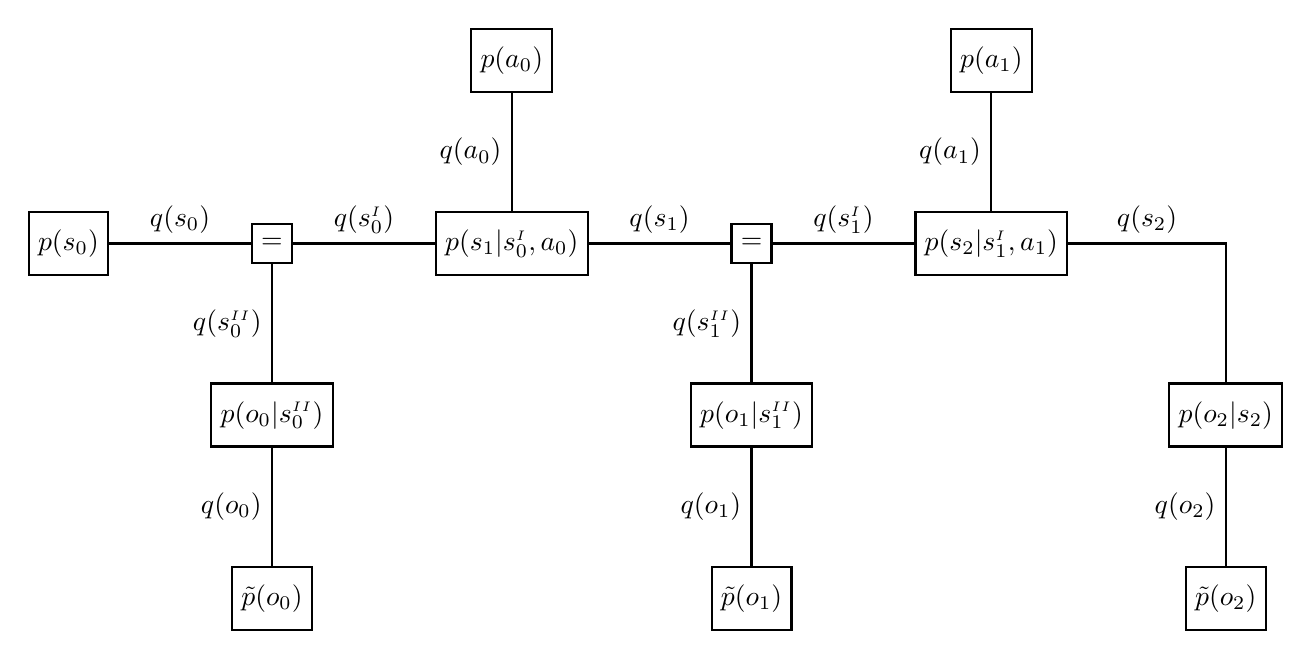
\begin{tikzpicture}[
                factor/.style={draw=black, thick, rectangle, minimum size=0.8cm, font=\normalsize},
                eqfactor/.style={draw=black, thick, rectangle, minimum size=0.5cm, font=\normalsize},
                edge/.style={thick},
                varlabel/.style={font=\normalsize},
                greycircle/.style={draw=black, thick, circle, fill=gray!30, minimum size=0.5cm, font=\normalsize}
            ]

            % Knoten
            \node[factor] (d) {$p(s_0)$};
            \node[eqfactor, right=1.8cm of d] (eq0) {$=$};
            \node[factor, below=1.5cm of eq0] (A0) {$p(o_0|s^{\scriptscriptstyle II}_0)$};
            \node[factor, below=1.5cm of A0] (c0) {$\tilde{p}(o_0)$};
            \node[factor, right=1.8cm of eq0] (B0) {$p(s_1|s^{\scriptscriptstyle I}_0,a_0)$};
            \node[eqfactor, right=1.8cm of B0] (eq1) {$=$};
            \node[factor, below=1.5cm of eq1] (A1) {$p(o_1|s^{\scriptscriptstyle II}_1)$};
            \node[factor, below=1.5cm of A1] (c1) {$\tilde{p}(o_1)$};
            \node[factor, right=1.8cm of eq1] (B1) {$p(s_2|s^{\scriptscriptstyle I}_1,a_1)$};
            \node[factor] (A2) at ([xshift=2cm] B1.east |- A1) {$p(o_2|s_2)$};
            \node[factor, below=1.5cm of A2] (c2) {$\tilde{p}(o_2)$};
            \node[factor, above=1.5cm of B0] (u0) {$p(a_0)$};
            \node[factor, above=1.5cm of B1] (u1) {$p(a_1)$};

            % Kanten zwischen Knoten
            \draw[edge] (d.east) -- (eq0.west) node[midway, above, varlabel] {$q(s_0)$};

            \draw[edge] (eq0.south) -- (A0.north) node[midway, left, varlabel] {$q(s^{\scriptscriptstyle II}_0)$};

            \draw[edge] (A0.south) -- (c0.north) node[midway, left, varlabel] {$q(o_0)$};

            \draw[edge] (eq0.east) -- (B0.west) node[midway, above, varlabel] {$q(s^{\scriptscriptstyle I}_0)$};

            \draw[edge] (B0.north) -- (u0.south) node[midway, left, varlabel] {$q(a_0)$};

            \draw[edge] (B0.east) -- (eq1.west) node[midway, above, varlabel] {$q(s_1)$};

            \draw[edge] (eq1.south) -- (A1.north) node[midway, left, varlabel] {$q(s^{\scriptscriptstyle II}_1)$};

            \draw[edge] (A1.south) -- (c1.north) node[midway, left, varlabel] {$q(o_1)$};

            \draw[edge] (eq1.east) -- (B1.west) node[midway, above, varlabel] {$q(s^{\scriptscriptstyle I}_1)$};

            \draw[edge] (B1.east) -| (A2.north) node[pos=0.25, above, varlabel] {$q(s_2)$};

            \draw[edge] (A2.south) -- (c2.north) node[midway, left, varlabel] {$q(o_2)$};

            \draw[edge] (B1.north) -- (u1.south) node[midway, left, varlabel] {$q(a_1)$};

            % Kanten an Knoten

        \end{tikzpicture}
    }

    \caption{Foundational Factor Graph of the two non-Context Agents.}
    \label{fig:8}
\end{figure}


\subsubsection{Lifecycle of an Agent}

The lifecycle of agents consists of three recurring stages (\cref{fig:30}): First, it receives an observation, which leads to a delta constraint at the respective belief distribution. For example, when the current timestep is \(t=0\) and it receives an observation \(\hat {o_0}\) then \(q(o_0)=\delta_{o_0,\hat {o_0}}\).

Second, the agent performs inference over the whole factor graph, i.e., the corresponding message passing algorithm is executed. In this way it computes the posterior distributions of all variables in the graph based on the observation \(\hat {o_0}\). These posteriors are then given by the respective belief distributions \(q\). In other words, during inference the agent forms beliefs about all variables in its graph. For example, it infers the hidden cause \(s_0\) of the observation \(\hat {o_0}\). Also, it infers a likely future trajectory of hidden states (via \(q(s_1)\) and \(q(s_2)\)). Moreover, it also forms beliefs about future observations. Crucially, these future observation beliefs are not solely driven by future hidden states but also by the preferences (i.e., \(\tilde{p}(o_1)\) and \(\tilde{p}(o_2)\)) on observations. The additional influence from the preferences couples back to other parts of graph such that the agent infers a future trajectory of hidden states that also leads to preferred observation. Moreover, it will also form appropriate action beliefs that fulfill these preferences.

In the third stage, the agent samples an action from the current action belief (e.g., \(q(a_0)\)) and "sends" it to the environment. In this work, the action belief will also be constrained by a delta distribution which enables the agent to "remember" which action it has executed.

After executing an action the cycle starts over again, i.e., the agent receives the next observation (\(\hat {o_1}\)). In this way, the agent collects observations from each timestep which remain as delta constraints in the factor graph. This enables the agent to remember past observations. Moreover, past beliefs about hidden states can still change when receiving new observations. This way, the agent can change its beliefs retrospectively. The other way around, past observations also influence the future trajectory of hidden states beliefs, i.e, the agent utilizes its memory of past events to make better predictions about the future.

% --- 1. GRAFIKEN ISOLIERT LADEN UND SKALIEREN ---
% Falls du die external-library in der Masterarbeit nutzt, hier kurz pausieren
\tikzexternaldisable

% Wir nutzen \scalebox, da es im Gegensatz zu TikZ-scale AUCH Label-Abstände schrumpft!
\newsavebox{\boxTL}
\sbox{\boxTL}{\scalebox{0.75}{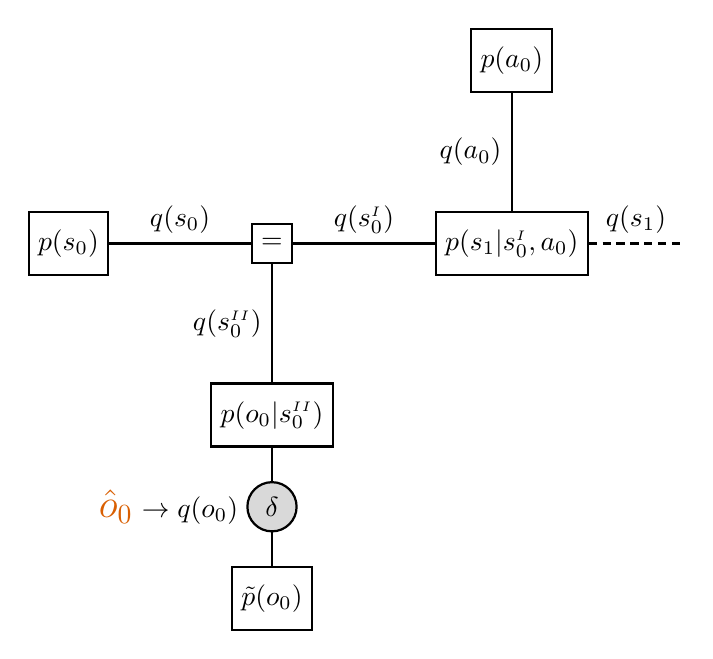
\begin{tikzpicture}[
    factor/.style={draw=black, thick, rectangle, minimum size=0.8cm, font=\normalsize, fill=white},
    eqfactor/.style={draw=black, thick, rectangle, minimum size=0.5cm, font=\normalsize, fill=white},
    edge/.style={thick},
    varlabel/.style={font=\normalsize},
    greycircle/.style={draw=black, thick, circle, fill=gray!30, minimum size=0.5cm, font=\normalsize}
]

% Knoten der linken Hälfte (t=0)
\node[factor] (d) {$p(s_0)$};
\node[eqfactor, right=1.8cm of d] (eq0) {$=$};
\node[factor, below=1.5cm of eq0] (A0) {$p(o_0|s^{\scriptscriptstyle II}_0)$};
\node[factor, below=1.5cm of A0] (c0) {$\tilde{p}(o_0)$};
\node[factor, right=1.8cm of eq0] (B0) {$p(s_1|s^{\scriptscriptstyle I}_0,a_0)$};
\node[factor, above=1.5cm of B0] (u0) {$p(a_0)$};

% Unsichtbarer Endpunkt für die ausgehende Kante
\coordinate[right=1.2cm of B0] (out_s1);

% Kanten
\draw[edge] (d.east) -- (eq0.west) node[midway, above, varlabel] {$q(s_0)$};
\draw[edge] (eq0.south) -- (A0.north) node[midway, left, varlabel] {$q(s^{\scriptscriptstyle II}_0)$};
\draw[edge] (A0.south) -- (c0.north) 
    node[midway, left=0.3cm, varlabel] {{\Large \textcolor{accorange}{$\hat{o}_0$}} $\rightarrow q(o_0)$} 
    node[midway, greycircle] {$\delta$};\draw[edge] (eq0.east) -- (B0.west) node[midway, above, varlabel] {$q(s^{\scriptscriptstyle I}_0)$};
\draw[edge] (B0.north) -- (u0.south) node[midway, left, varlabel] {$q(a_0)$};

% Abgebrochene Kante, die anzeigt, dass der Graph weitergeht (optional gestrichelt)
\draw[edge, densely dashed] (B0.east) -- (out_s1) node[midway, above, varlabel] {$q(s_1)$};

\end{tikzpicture}}}

\newsavebox{\boxTR}
\sbox{\boxTR}{\scalebox{0.75}{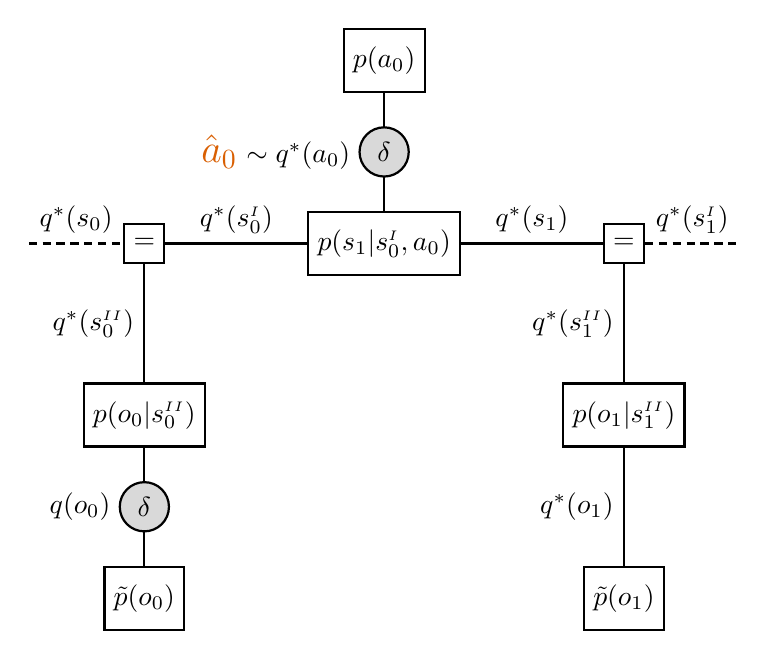
\begin{tikzpicture}[
    factor/.style={draw=black, thick, rectangle, minimum size=0.8cm, font=\normalsize, fill=white},
    eqfactor/.style={draw=black, thick, rectangle, minimum size=0.5cm, font=\normalsize, fill=white},
    edge/.style={thick},
    varlabel/.style={font=\normalsize},
    greycircle/.style={draw=black, thick, circle, fill=gray!30, minimum size=0.5cm, font=\normalsize}
]

% --- KNOTEN ---
% Wir starten mit eq0 als "Anker" für diesen Ausschnitt
\node[eqfactor] (eq0) {$=$};

% Knoten t=0 (unterhalb eq0)
\node[factor, below=1.5cm of eq0] (A0) {$p(o_0|s^{\scriptscriptstyle II}_0)$};
\node[factor, below=1.5cm of A0] (c0) {$\tilde{p}(o_0)$};

% Übergang & Knoten t=1
\node[factor, right=1.8cm of eq0] (B0) {$p(s_1|s^{\scriptscriptstyle I}_0,a_0)$};
\node[factor, above=1.5cm of B0] (u0) {$p(a_0)$};

\node[eqfactor, right=1.8cm of B0] (eq1) {$=$};
\node[factor, below=1.5cm of eq1] (A1) {$p(o_1|s^{\scriptscriptstyle II}_1)$};
\node[factor, below=1.5cm of A1] (c1) {$\tilde{p}(o_1)$};

% Unsichtbare Koordinaten für die gestrichelten Enden links und rechts
\coordinate[left=1.2cm of eq0] (in_s0);
\coordinate[right=1.2cm of eq1] (out_sI1);


% --- KANTEN ---

% 1. Gestrichelte Eingangskante q(s_0)
\draw[edge, densely dashed] (in_s0) -- (eq0.west) node[midway, above, varlabel] {$q^*(s_0)$};

% 2. Durchgezogene innere Kanten
\draw[edge] (eq0.south) -- (A0.north) node[midway, left, varlabel] {$q^*(s^{\scriptscriptstyle II}_0)$};
\draw[edge] (A0.south) -- (c0.north) node[midway, left=0.3, varlabel] {$q(o_0)$} node[midway, greycircle] {$\delta$};

\draw[edge] (eq0.east) -- (B0.west) node[midway, above, varlabel] {$q^*(s^{\scriptscriptstyle I}_0)$};
\draw[edge] (B0.north) -- (u0.south) node[midway, left=0.3cm, varlabel] {{\Large \textcolor{accorange}{$\hat{a}_0$}} $\sim q^*(a_0)$} node[midway, greycircle] {$\delta$};
\draw[edge] (B0.east) -- (eq1.west) node[midway, above, varlabel] {$q^*(s_1)$};

\draw[edge] (eq1.south) -- (A1.north) node[midway, left, varlabel] {$q^*(s^{\scriptscriptstyle II}_1)$};
\draw[edge] (A1.south) -- (c1.north) node[midway, left, varlabel] {$q^*(o_1)$};

% 3. Gestrichelte Ausgangskante q(s^I_1)
\draw[edge, densely dashed] (eq1.east) -- (out_sI1) node[midway, above, varlabel] {$q^*(s^{\scriptscriptstyle I}_1)$};

\end{tikzpicture}}}

\newsavebox{\boxBOT}
\sbox{\boxBOT}{\scalebox{0.75}{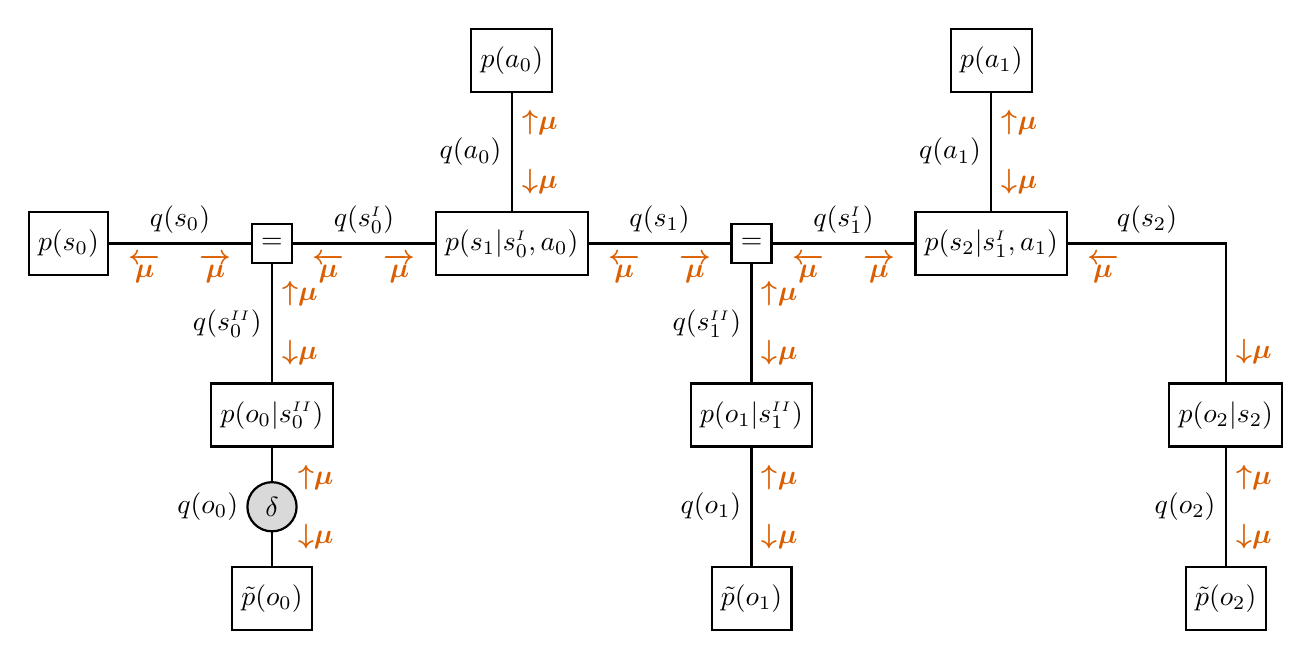
\begin{tikzpicture}[
    factor/.style={draw=black, thick, rectangle, minimum size=0.8cm, font=\normalsize, fill=white},
    eqfactor/.style={draw=black, thick, rectangle, minimum size=0.5cm, font=\normalsize, fill=white},
    edge/.style={thick},
    varlabel/.style={font=\normalsize},
    greycircle/.style={draw=black, thick, circle, fill=gray!30, minimum size=0.5cm, font=\normalsize}
]

% Knoten
\node[factor] (d) {$p(s_0)$};
\node[eqfactor, right=1.8cm of d] (eq0) {$=$};
\node[factor, below=1.5cm of eq0] (A0) {$p(o_0|s^{\scriptscriptstyle II}_0)$};
\node[factor, below=1.5cm of A0] (c0) {$\tilde{p}(o_0)$};
\node[factor, right=1.8cm of eq0] (B0) {$p(s_1|s^{\scriptscriptstyle I}_0,a_0)$};
\node[eqfactor, right=1.8cm of B0] (eq1) {$=$};
\node[factor, below=1.5cm of eq1] (A1) {$p(o_1|s^{\scriptscriptstyle II}_1)$};
\node[factor, below=1.5cm of A1] (c1) {$\tilde{p}(o_1)$};
\node[factor, right=1.8cm of eq1] (B1) {$p(s_2|s^{\scriptscriptstyle I}_1,a_1)$};
\node[factor] (A2) at ([xshift=2cm] B1.east |- A1) {$p(o_2|s_2)$};
\node[factor, below=1.5cm of A2] (c2) {$\tilde{p}(o_2)$};
\node[factor, above=1.5cm of B0] (u0) {$p(a_0)$};
\node[factor, above=1.5cm of B1] (u1) {$p(a_1)$};

% Kanten zwischen Knoten
\draw[edge] (d.east) -- (eq0.west) node[midway, above, varlabel] {$q(s_0)$} node[near end, below, varlabel] {$\textcolor{accorange}{\bm{\overrightarrow{\mu}}}$} node[near start, below, varlabel] {$\textcolor{accorange}{\bm{\overleftarrow{\mu}}}$};
\draw[edge] (eq0.south) -- (A0.north) node[midway, left, varlabel] {$q(s^{\scriptscriptstyle II}_0)$} node[near start, right, varlabel] {$\textcolor{accorange}{\bm{{\uparrow}{\mu}}}$} node[near end, right, varlabel] {$\textcolor{accorange}{\bm{{\downarrow}{\mu}}}$};
\draw[edge] (A0.south) -- (c0.north) node[midway, left=0.3, varlabel] {$q(o_0)$} node[midway, greycircle] {$\delta$} node[near start, right=0.2, varlabel] {$\textcolor{accorange}{\bm{{\uparrow}{\mu}}}$} node[near end, right=0.2, varlabel] {$\textcolor{accorange}{\bm{{\downarrow}{\mu}}}$};
\draw[edge] (eq0.east) -- (B0.west) node[midway, above, varlabel] {$q(s^{\scriptscriptstyle I}_0)$} node[near end, below, varlabel] {$\textcolor{accorange}{\bm{\overrightarrow{\mu}}}$} node[near start, below, varlabel] {$\textcolor{accorange}{\bm{\overleftarrow{\mu}}}$};
\draw[edge] (B0.north) -- (u0.south) node[midway, left, varlabel] {$q(a_0)$} node[near end, right, varlabel] {$\textcolor{accorange}{\bm{{\uparrow}{\mu}}}$} node[near start, right, varlabel] {$\textcolor{accorange}{\bm{{\downarrow}{\mu}}}$};
\draw[edge] (B0.east) -- (eq1.west) node[midway, above, varlabel] {$q(s_1)$} node[near end, below, varlabel] {$\textcolor{accorange}{\bm{\overrightarrow{\mu}}}$} node[near start, below, varlabel] {$\textcolor{accorange}{\bm{\overleftarrow{\mu}}}$};
\draw[edge] (eq1.south) -- (A1.north) node[midway, left, varlabel] {$q(s^{\scriptscriptstyle II}_1)$} node[near start, right, varlabel] {$\textcolor{accorange}{\bm{{\uparrow}{\mu}}}$} node[near end, right, varlabel] {$\textcolor{accorange}{\bm{{\downarrow}{\mu}}}$};
\draw[edge] (A1.south) -- (c1.north) node[midway, left, varlabel] {$q(o_1)$} node[near start, right, varlabel] {$\textcolor{accorange}{\bm{{\uparrow}{\mu}}}$} node[near end, right, varlabel] {$\textcolor{accorange}{\bm{{\downarrow}{\mu}}}$};
\draw[edge] (eq1.east) -- (B1.west) node[midway, above, varlabel] {$q(s^{\scriptscriptstyle I}_1)$} node[near end, below, varlabel] {$\textcolor{accorange}{\bm{\overrightarrow{\mu}}}$} node[near start, below, varlabel] {$\textcolor{accorange}{\bm{\overleftarrow{\mu}}}$};
\draw[edge] (B1.east) -| (A2.north) node[pos=0.25, above, varlabel] {$q(s_2)$} node[pos=0.11, below, varlabel] {$\textcolor{accorange}{\bm{\overleftarrow{\mu}}}$} node[pos=0.89, right, varlabel] {$\textcolor{accorange}{\bm{{\downarrow}{\mu}}}$};
\draw[edge] (A2.south) -- (c2.north) node[midway, left, varlabel] {$q(o_2)$} node[near start, right, varlabel] {$\textcolor{accorange}{\bm{{\uparrow}{\mu}}}$} node[near end, right, varlabel] {$\textcolor{accorange}{\bm{{\downarrow}{\mu}}}$};
\draw[edge] (B1.north) -- (u1.south) node[midway, left, varlabel] {$q(a_1)$} node[near end, right, varlabel] {$\textcolor{accorange}{\bm{{\uparrow}{\mu}}}$} node[near start, right, varlabel] {$\textcolor{accorange}{\bm{{\downarrow}{\mu}}}$};

\end{tikzpicture}}}


% --- 2. DAS LAYOUT ZUSAMMENSETZEN ---
\begin{figure}[htbp]
    \centering
    \resizebox{1.0\textwidth}{!}{%
        \begin{tikzpicture}[
                >=Stealth,
                % Hier definieren wir die blauen Boxen. Die runden Ecken hier 
                % können jetzt NICHT mehr in deine Faktorgraphen durchbluten.
                panel/.style={
                        draw=gray!80, thick, fill=blue!5,
                        rounded corners=4pt, inner sep=8pt, align=center
                    },
                cycle arrow/.style={
                        ->, line width=2.0pt, color=gray!80!black
                    }
            ]

            % Die vorbereiteten, perfekt skalierten Boxen einfügen
            \node[panel] (TL) at (0,0) {\usebox{\boxTL}};

            \node[panel, right=0.5cm of TL] (TR) {\usebox{\boxTR}};

            \path (TL.south west) -- (TR.south east) coordinate[midway] (centerBottom);
            \node[panel, below=0.5cm of centerBottom, anchor=north] (BOT) {\usebox{\boxBOT}};

            % --- NEU: Freischwebender Text IN den Boxen (oben rechts) ---
            % xshift und yshift rücken den Text etwas vom Rand weg nach innen.
            \node[anchor=north west, font=\sffamily\bfseries\normalsize, text=gray!80!black]
            at ([xshift=8pt, yshift=-8pt]TL.north west) {Perception};

            \node[anchor=north west, font=\sffamily\bfseries\normalsize, text=gray!80!black]
            at ([xshift=8pt, yshift=-8pt]TR.north west) {Action};

            \node[anchor=north west, font=\sffamily\bfseries\normalsize, text=gray!80!black]
            at ([xshift=8pt, yshift=-8pt]BOT.north west) {Inference};
            % -------------------------------------------------------------

            % Die Pfeile außen herum
            \draw[cycle arrow, dashed] (TR.north) to[bend right=20]
            node[midway, above=4pt, font=\sffamily\bfseries] {} (TL.north);

            \draw[cycle arrow] (TL.west) to[bend right=35]
            node[midway, left=4pt, font=\sffamily\bfseries] {} (BOT.west);

            \draw[cycle arrow] (BOT.east) to[bend right=35]
            node[midway, right=4pt, font=\sffamily\bfseries] {} (TR.east);

        \end{tikzpicture}
    }

    \tikzexternalenable

    \caption{Agents' lifecycle with the recurring stages perception, inference, and action. During perception the observation belief that corresponds to the current timestep (e.g., \(q(o_0\)) becomes a delta distribution with all probability mass at the actual observation \(\hat{o_0}\). When performing inference the messages are sent on the edges (message passing) and all belief distributions are updated (indicated by \(q^*\)) (expect the delta constrained distributions). During action, an action \(\hat{a_0}\) is sampled from the corresponding belief distribution \(q(a_0)\) that has been infered during inference. Additionally, this belief also becomes a delta distribution with all probability mass on the sampled action \(\hat{a_0}\). After an action, the cycle starts over again and the next observation (e.g., \(\hat{o_1}\)) is perceived.}
    \label{fig:30}
\end{figure}

The POMDP in \cref{eq:15} and the corresponding factor graph in \cref{fig:8} will be the basis for the BFE- and GFE agents that are introduced in following sections.


\subsection{Bethe Free Energy (BFE) Agent}

In this section I present the message passing algorithm of the BFE agent. This agent serves as a baseline without having an additional context layer nor does it do information seeking. All messages can be derived from the Bethe free energy of its factor graph (compare \cref{sec:1}). Messages from equality nodes also result from the Bethe free energy (see \cref{app:1}). The agent's generative model is given by \cref{eq:15}.

\subsubsection{Message Passing Algorithm}

The factor graph that results from the POMDP is given in \cref{fig:31} (including variable beliefs and messages) and the corresponding message passing algorithm that enables inference is given in \cref{alg:2}. Note that in the graph the agent has already received an observation \(\hat {o_0}\) to exemplify the alternative messages resulting from the corresponding delta constraint.

\begin{figure}[htbp]
    \centering

    \resizebox{1.0\textwidth}{!}{%
        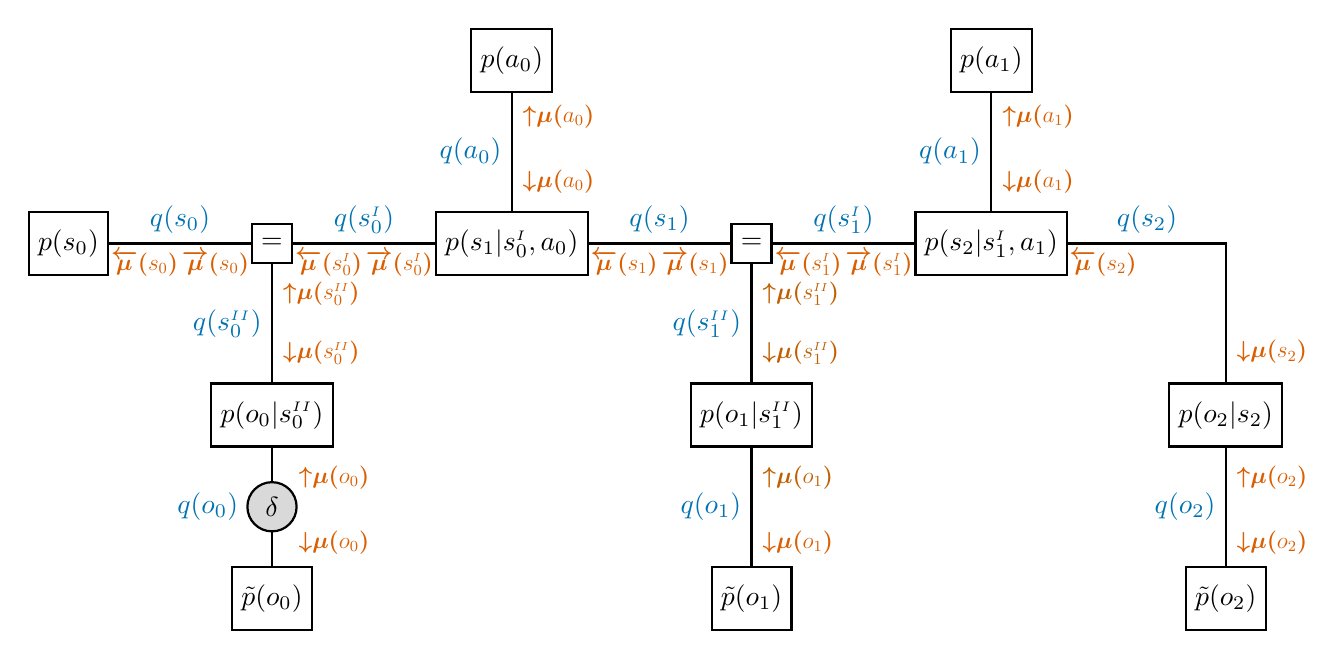
\begin{tikzpicture}[
                factor/.style={draw=black, thick, rectangle, minimum size=0.8cm, font=\normalsize},
                eqfactor/.style={draw=black, thick, rectangle, minimum size=0.5cm, font=\normalsize},
                edge/.style={thick},
                varlabel/.style={font=\normalsize},
                greycircle/.style={draw=black, thick, circle, fill=gray!30, minimum size=0.5cm, font=\normalsize}
            ]

            % Knoten
            \node[factor] (d) {$p(s_0)$};
            \node[eqfactor, right=1.8cm of d] (eq0) {$=$};
            \node[factor, below=1.5cm of eq0] (A0) {$p(o_0|s^{\scriptscriptstyle II}_0)$};
            \node[factor, below=1.5cm of A0] (c0) {$\tilde{p}(o_0)$};
            \node[factor, right=1.8cm of eq0] (B0) {$p(s_1|s^{\scriptscriptstyle I}_0,a_0)$};
            \node[eqfactor, right=1.8cm of B0] (eq1) {$=$};
            \node[factor, below=1.5cm of eq1] (A1) {$p(o_1|s^{\scriptscriptstyle II}_1)$};
            \node[factor, below=1.5cm of A1] (c1) {$\tilde{p}(o_1)$};
            \node[factor, right=1.8cm of eq1] (B1) {$p(s_2|s^{\scriptscriptstyle I}_1,a_1)$};
            \node[factor] (A2) at ([xshift=2cm] B1.east |- A1) {$p(o_2|s_2)$};
            \node[factor, below=1.5cm of A2] (c2) {$\tilde{p}(o_2)$};
            \node[factor, above=1.5cm of B0] (u0) {$p(a_0)$};
            \node[factor, above=1.5cm of B1] (u1) {$p(a_1)$};

            % Kanten zwischen Knoten
            \draw[edge] (d.east) -- (eq0.west) node[midway, above, varlabel] {$\textcolor{accblue}{q(s_0)}$} node[near end, below, varlabel, scale=0.7] {${\large \textcolor{accorange}{\bm{\overrightarrow{\mu}(}s_0\bm{)}}}$} node[near start, below, varlabel, scale=0.7] {${\large \textcolor{accorange}{\bm{\overleftarrow{\mu}(}s_0\bm{)}}}$};
            \draw[edge] (eq0.south) -- (A0.north) node[midway, left, varlabel] {$\textcolor{accblue}{q(s^{\scriptscriptstyle II}_0)}$} node[pos=0.25, right=0.05, varlabel, scale=0.7] {${\large \textcolor{accorange}{\bm{{\uparrow}{\mu}(}s^{\scriptscriptstyle II}_0\bm{)}}}$} node[pos=0.75, right=0.05, varlabel, scale=0.7] {${\large \textcolor{accorange}{\bm{{\downarrow}{\mu}(}s^{\scriptscriptstyle II}_0\bm{)}}}$};
            \draw[edge] (A0.south) -- (c0.north) node[midway, greycircle] {$\delta$} node[midway, left=0.3, varlabel] {$\textcolor{accblue}{q(o_0)}$} node[pos=0.25, right=0.25, varlabel, scale=0.7] {${\large \textcolor{accorange}{\bm{{\uparrow}{\mu}(}o_0\bm{)}}}$} node[pos=0.8, right=0.25, varlabel, scale=0.7] {${\large \textcolor{accorange}{\bm{{\downarrow}{\mu}(}o_0\bm{)}}}$};
            \draw[edge] (eq0.east) -- (B0.west) node[midway, above, varlabel] {$\textcolor{accblue}{q(s^{\scriptscriptstyle I}_0)}$} node[near start, below, varlabel, scale=0.7] {${\large \textcolor{accorange}{\bm{\overleftarrow{\mu}(}s^{\scriptscriptstyle I}_0\bm{)}}}$} node[near end, below, varlabel, scale=0.7] {${\large \textcolor{accorange}{\bm{\overrightarrow{\mu}(}s^{\scriptscriptstyle I}_0\bm{)}}}$};
            \draw[edge] (B0.north) -- (u0.south) node[midway, left, varlabel] {$\textcolor{accblue}{q(a_0)}$} node[pos=0.25, right=0.05, varlabel, scale=0.7] {${\large \textcolor{accorange}{\bm{{\downarrow}{\mu}(}a_0\bm{)}}}$} node[pos=0.8, right=0.05, varlabel, scale=0.7] {${\large \textcolor{accorange}{\bm{{\uparrow}{\mu}(}a_0\bm{)}}}$};
            \draw[edge] (B0.east) -- (eq1.west) node[midway, above, varlabel] {$\textcolor{accblue}{q(s_1)}$} node[near end, below, varlabel, scale=0.7] {${\large \textcolor{accorange}{\bm{\overrightarrow{\mu}(}s_1\bm{)}}}$} node[near start, below, varlabel, scale=0.7] {${\large \textcolor{accorange}{\bm{\overleftarrow{\mu}(}s_1\bm{)}}}$};
            \draw[edge] (eq1.south) -- (A1.north) node[midway, left, varlabel] {$\textcolor{accblue}{q(s^{\scriptscriptstyle II}_1)}$} node[pos=0.25, right=0.05, varlabel, scale=0.7] {${\large \textcolor{orange!75!black}{\bm{{\uparrow}{\mu}(}s^{\scriptscriptstyle II}_1\bm{)}}}$} node[pos=0.75, right=0.05, varlabel, scale=0.7] {${\large \textcolor{orange!75!black}{\bm{{\downarrow}{\mu}(}s^{\scriptscriptstyle II}_1\bm{)}}}$};
            \draw[edge] (A1.south) -- (c1.north) node[midway, left, varlabel] {$\textcolor{accblue}{q(o_1)}$} node[pos=0.25, right=0.05, varlabel, scale=0.7] {${\large \textcolor{orange!75!black}{\bm{{\uparrow}{\mu}(}o_1\bm{)}}}$} node[pos=0.8, right=0.05, varlabel, scale=0.7] {${\large \textcolor{accorange}{\bm{{\downarrow}{\mu}(}o_1\bm{)}}}$};
            \draw[edge] (eq1.east) -- (B1.west) node[midway, above, varlabel] {$\textcolor{accblue}{q(s^{\scriptscriptstyle I}_1)}$} node[near start, below, varlabel, scale=0.7] {${\large \textcolor{accorange}{\bm{\overleftarrow{\mu}(}s^{\scriptscriptstyle I}_1\bm{)}}}$} node[near end, below, varlabel, scale=0.7] {${\large \textcolor{accorange}{\bm{\overrightarrow{\mu}(}s^{\scriptscriptstyle I}_1\bm{)}}}$};
            \draw[edge] (B1.east) -| (A2.north) node[pos=0.25, above, varlabel] {$\textcolor{accblue}{q(s_2)}$} node[pos=0.89, right=0.05, varlabel, scale=0.7] {${\large \textcolor{accorange}{\bm{{\downarrow}{\mu}(}s_2\bm{)}}}$} node[pos=0.11, below, varlabel, scale=0.7] {${\large \textcolor{accorange}{\bm{\overleftarrow{\mu}(}s_2\bm{)}}}$};
            \draw[edge] (A2.south) -- (c2.north) node[midway, left, varlabel] {$\textcolor{accblue}{q(o_2)}$} node[pos=0.25, right=0.05, varlabel, scale=0.7] {${\large \textcolor{accorange}{\bm{{\uparrow}{\mu}(}o_2\bm{)}}}$} node[pos=0.8, right=0.05, varlabel, scale=0.7] {${\large \textcolor{accorange}{\bm{{\downarrow}{\mu}(}o_2\bm{)}}}$};
            \draw[edge] (B1.north) -- (u1.south) node[midway, left, varlabel] {$\textcolor{accblue}{q(a_1)}$} node[pos=0.25, right=0.05, varlabel, scale=0.7] {${\large \textcolor{accorange}{\bm{{\downarrow}{\mu}(}a_1\bm{)}}}$} node[pos=0.8, right=0.05, varlabel, scale=0.7] {${\large \textcolor{accorange}{\bm{{\uparrow}{\mu}(}a_1\bm{)}}}$};

        \end{tikzpicture}
    }

    \caption{Factor graph of the BFE agent with variables' belief distributions \(\textcolor{accblue}{q}\) and messages \(\textcolor{accorange}{\mu}\).}
    \label{fig:31}
\end{figure}

\begin{algorithm}[htbp]
    \caption{Message Passing Algorithm of the BFE Agent}
    \label{alg:2}
    \small
    \begin{algorithmic}[1] % Die [1] sorgt für automatische Zeilennummern!
        \linespread{1.4}\selectfont
        \State $\textcolor{accorange}{\bm{\overrightarrow{\mu}(}s_0\bm{)}} \propto p(s_0)$,\quad$\textcolor{accorange}{\bm{{\uparrow}{\mu}(}o_0\bm{)}} \propto \delta_{o_0,\hat{o_0}}$,\quad$\textcolor{accorange}{\bm{{\downarrow}{\mu}(}a_0\bm{)}} \propto p(a_0)$,\quad$\textcolor{accorange}{\bm{{\uparrow}{\mu}(}o_1\bm{)}} \propto \tilde{p}(o_1)$,\quad$\textcolor{accorange}{\bm{{\downarrow}{\mu}(}a_1\bm{)}} \propto p(a_1)$,
        \Statex $\textcolor{accorange}{\bm{{\uparrow}{\mu}(}o_2\bm{)}} \propto \tilde{p}(o_2)$,\quad$\textcolor{accorange}{\bm{{\downarrow}{\mu}(}o_0\bm{)}} \propto \delta_{o_0,\hat{o_0}}$
        \State $\textcolor{accorange}{\bm{{\uparrow}{\mu}(}s^{\scriptscriptstyle II}_0\bm{)}} \propto \sum_{o_0} p(o_0|s^{\scriptscriptstyle II}_0) \textcolor{black}{\bm{{\uparrow}{\mu}(}o_0\bm{)}}$,\quad$\textcolor{accorange}{\bm{{\uparrow}{\mu}(}s^{\scriptscriptstyle II}_1\bm{)}} \propto \sum_{o_1} p(o_1|s^{\scriptscriptstyle II}_1) \textcolor{black}{\bm{{\uparrow}{\mu}(}o_1\bm{)}}$,
        \Statex $\textcolor{accorange}{\bm{\overleftarrow{\mu}(}s_2\bm{)}} \propto \sum_{o_2} p(o_2|s_2) \textcolor{black}{\bm{{\uparrow}{\mu}(}o_2\bm{)}}$
        \State $\textcolor{accorange}{\bm{\overrightarrow{\mu}(}s^{\scriptscriptstyle I}_0\bm{)}} \propto \sum_{s_0,s^{\scriptscriptstyle II}_0} \delta_{s_0,s^{\scriptscriptstyle I}_0}\delta_{s_0,s^{\scriptscriptstyle II}_0} \textcolor{black}{\bm{\overrightarrow{\mu}(}s_0\bm{)}} \textcolor{black}{\bm{{\uparrow}{\mu}(}s^{\scriptscriptstyle II}_0\bm{)}}$,\quad$\textcolor{accorange}{\bm{\overleftarrow{\mu}(}s^{\scriptscriptstyle I}_1\bm{)}} \propto \sum_{a_1,s_2} p(s_2|s^{\scriptscriptstyle I}_1,a_1) \textcolor{black}{\bm{{\downarrow}{\mu}(}a_1\bm{)}} \textcolor{black}{\bm{\overleftarrow{\mu}(}s_2\bm{)}}$
        \State $\textcolor{accorange}{\bm{\overrightarrow{\mu}(}s_1\bm{)}} \propto \sum_{s^{\scriptscriptstyle I}_0,a_0} p(s_1|s^{\scriptscriptstyle I}_0,a_0) \textcolor{black}{\bm{\overrightarrow{\mu}(}s^{\scriptscriptstyle I}_0\bm{)}} \textcolor{black}{\bm{{\downarrow}{\mu}(}a_0\bm{)}}$,\quad$\textcolor{accorange}{\bm{\overleftarrow{\mu}(}s_1\bm{)}} \propto \sum_{s^{\scriptscriptstyle I}_1,s^{\scriptscriptstyle II}_1} \delta_{s_1,s^{\scriptscriptstyle I}_1}\delta_{s_1,s^{\scriptscriptstyle II}_1} \textcolor{black}{\bm{\overleftarrow{\mu}(}s^{\scriptscriptstyle I}_1\bm{)}} \textcolor{black}{\bm{{\uparrow}{\mu}(}s^{\scriptscriptstyle II}_1\bm{)}}$
        \State $\textcolor{accorange}{\bm{\overrightarrow{\mu}(}s^{\scriptscriptstyle I}_1\bm{)}} \propto \sum_{s_1,s^{\scriptscriptstyle II}_1} \delta_{s_1,s^{\scriptscriptstyle I}_1}\delta_{s_1,s^{\scriptscriptstyle II}_1} \textcolor{black}{\bm{\overrightarrow{\mu}(}s_1\bm{)}} \textcolor{black}{\bm{{\uparrow}{\mu}(}s^{\scriptscriptstyle II}_1\bm{)}}$,\quad$\textcolor{accorange}{\bm{{\downarrow}{\mu}(}s^{\scriptscriptstyle II}_1\bm{)}} \propto \sum_{s_1,s^{\scriptscriptstyle I}_1} \delta_{s_1,s^{\scriptscriptstyle I}_1}\delta_{s_1,s^{\scriptscriptstyle II}_1} \textcolor{black}{\bm{\overrightarrow{\mu}(}s_1\bm{)}} \textcolor{black}{\bm{\overleftarrow{\mu}(}s^{\scriptscriptstyle I}_1\bm{)}}$,
        \Statex $\textcolor{accorange}{\bm{{\uparrow}{\mu}(}a_0\bm{)}} \propto \sum_{s_1,s^{\scriptscriptstyle I}_0} p(s_1|s^{\scriptscriptstyle I}_0,a_0) \textcolor{black}{\bm{\overrightarrow{\mu}(}s^{\scriptscriptstyle I}_0\bm{)}} \textcolor{black}{\bm{\overleftarrow{\mu}(}s_1\bm{)}}$,\quad$\textcolor{accorange}{\bm{\overleftarrow{\mu}(}s^{\scriptscriptstyle I}_0\bm{)}} \propto \sum_{s_1,a_0} p(s_1|s^{\scriptscriptstyle I}_0,a_0) \textcolor{black}{\bm{{\downarrow}{\mu}(}a_0\bm{)}} \textcolor{black}{\bm{\overleftarrow{\mu}(}s_1\bm{)}}$
        \State $\textcolor{accorange}{\bm{{\uparrow}{\mu}(}a_1\bm{)}} \propto \sum_{s^{\scriptscriptstyle I}_1,s_2} p(s_2|s^{\scriptscriptstyle I}_1,a_1) \textcolor{black}{\bm{\overrightarrow{\mu}(}s^{\scriptscriptstyle I}_1\bm{)}} \textcolor{black}{\bm{\overleftarrow{\mu}(}s_2\bm{)}}$,\quad$\textcolor{accorange}{\bm{{\downarrow}{\mu}(}s_2\bm{)}} \propto \sum_{s^{\scriptscriptstyle I}_1,a_1} p(s_2|s^{\scriptscriptstyle I}_1,a_1) \textcolor{black}{\bm{\overrightarrow{\mu}(}s^{\scriptscriptstyle I}_1\bm{)}} \textcolor{black}{\bm{{\downarrow}{\mu}(}a_1\bm{)}}$,
        \Statex $\textcolor{accorange}{\bm{\overleftarrow{\mu}(}s_0\bm{)}} \propto \sum_{s^{\scriptscriptstyle I}_0,s^{\scriptscriptstyle II}_0} \delta_{s_0,s^{\scriptscriptstyle I}_0}\delta_{s_0,s^{\scriptscriptstyle II}_0} \textcolor{black}{\bm{\overleftarrow{\mu}(}s^{\scriptscriptstyle I}_0\bm{)}} \textcolor{black}{\bm{{\uparrow}{\mu}(}s^{\scriptscriptstyle II}_0\bm{)}}$,\quad$\textcolor{accorange}{\bm{{\downarrow}{\mu}(}s^{\scriptscriptstyle II}_0\bm{)}} \propto \sum_{s_0,s^{\scriptscriptstyle I}_0} \delta_{s_0,s^{\scriptscriptstyle I}_0}\delta_{s_0,s^{\scriptscriptstyle II}_0} \textcolor{black}{\bm{\overrightarrow{\mu}(}s_0\bm{)}} \textcolor{black}{\bm{\overleftarrow{\mu}(}s^{\scriptscriptstyle I}_0\bm{)}}$,
        \Statex $\textcolor{accorange}{\bm{{\downarrow}{\mu}(}o_1\bm{)}} \propto \sum_{s^{\scriptscriptstyle II}_1} p(o_1|s^{\scriptscriptstyle II}_1) \textcolor{black}{\bm{{\downarrow}{\mu}(}s^{\scriptscriptstyle II}_1\bm{)}}$
        \State $\textcolor{accorange}{\bm{{\downarrow}{\mu}(}o_2\bm{)}} \propto \sum_{s_2} p(o_2|s_2) \textcolor{black}{\bm{{\downarrow}{\mu}(}s_2\bm{)}}$
        \State $\textcolor{accblue}{q(s_0)} \propto \textcolor{black}{\bm{\overleftarrow{\mu}(}s_0\bm{)}} \textcolor{black}{\bm{\overrightarrow{\mu}(}s_0\bm{)}}$,\quad$\textcolor{accblue}{q(s^{\scriptscriptstyle I}_0)} \propto \textcolor{black}{\bm{\overleftarrow{\mu}(}s^{\scriptscriptstyle I}_0\bm{)}} \textcolor{black}{\bm{\overrightarrow{\mu}(}s^{\scriptscriptstyle I}_0\bm{)}}$,\quad$\textcolor{accblue}{q(s^{\scriptscriptstyle II}_0)} \propto \textcolor{black}{\bm{{\uparrow}{\mu}(}s^{\scriptscriptstyle II}_0\bm{)}} \textcolor{black}{\bm{{\downarrow}{\mu}(}s^{\scriptscriptstyle II}_0\bm{)}}$,
        \Statex $\textcolor{accblue}{q(s_1)} \propto \textcolor{black}{\bm{\overleftarrow{\mu}(}s_1\bm{)}} \textcolor{black}{\bm{\overrightarrow{\mu}(}s_1\bm{)}}$,\quad$\textcolor{accblue}{q(s^{\scriptscriptstyle I}_1)} \propto \textcolor{black}{\bm{\overleftarrow{\mu}(}s^{\scriptscriptstyle I}_1\bm{)}} \textcolor{black}{\bm{\overrightarrow{\mu}(}s^{\scriptscriptstyle I}_1\bm{)}}$,\quad$\textcolor{accblue}{q(s^{\scriptscriptstyle II}_1)} \propto \textcolor{black}{\bm{{\uparrow}{\mu}(}s^{\scriptscriptstyle II}_1\bm{)}} \textcolor{black}{\bm{{\downarrow}{\mu}(}s^{\scriptscriptstyle II}_1\bm{)}}$,
        \Statex $\textcolor{accblue}{q(s_2)} \propto \textcolor{black}{\bm{\overleftarrow{\mu}(}s_2\bm{)}} \textcolor{black}{\bm{{\downarrow}{\mu}(}s_2\bm{)}}$,\quad$\textcolor{accblue}{q(a_0)} \propto \textcolor{black}{\bm{{\uparrow}{\mu}(}a_0\bm{)}} \textcolor{black}{\bm{{\downarrow}{\mu}(}a_0\bm{)}}$,\quad$\textcolor{accblue}{q(a_1)} \propto \textcolor{black}{\bm{{\uparrow}{\mu}(}a_1\bm{)}} \textcolor{black}{\bm{{\downarrow}{\mu}(}a_1\bm{)}}$,
        \Statex $\textcolor{accblue}{q(o_0)} \propto \textcolor{black}{\bm{{\uparrow}{\mu}(}o_0\bm{)}} \textcolor{black}{\bm{{\downarrow}{\mu}(}o_0\bm{)}}$,\quad$\textcolor{accblue}{q(o_1)} \propto \textcolor{black}{\bm{{\uparrow}{\mu}(}a_1\bm{)}} \textcolor{black}{\bm{{\downarrow}{\mu}(}a_1\bm{)}}$,\quad$\textcolor{accblue}{q(o_2)} \propto \textcolor{black}{\bm{{\uparrow}{\mu}(}a_2\bm{)}} \textcolor{black}{\bm{{\downarrow}{\mu}(}a_2\bm{)}}$
    \end{algorithmic}
\end{algorithm}



\subsection{Generalized Free Energy (GFE) Agent}
\label{sec:gfe}

In this section I introduce the GFE agent. It can be considered a real Active Inference agent because it does not solely minimize the Bethe free energy but also respects additional motives that lead to information seeking. This makes up for the generalized free energy that Active Inference agents are mandated to minimize. The GFE agent is indeed similar to the BFE agent and is also based on the same generative model (\cref{eq:15}) but instead of only realizing preferred observations it also seeks information in the environment, i.e., it is curious. In other words, during inference it infers actions that do not only lead to preferred observation \(o\) but which are also informative regarding the hidden states \(s\) of its generative model. The amount of information that a certain observation yields with respect to its hidden state (that the agent assumes to generate this observation via its generative model) can be quantified via the mutual information between these two variables. Formally, the GFE agent is driven to maximize the mutual information between future hidden state beliefs \(q(s)\) and observation beliefs \(q(o)\). This mechanism enables it to sample actions at present time that maximize this quantity. The mechanism is encoded in the free energy functional (Lagrangian) of the agent and leads to alternative messages at the edges in the corresponding factor graph that resemble future hidden states. Moreover, we will see that messages at edges of future observation beliefs disappear under this motive. Importantly, the mutual information mechanism is only applied to future parts of the factor graph, i.e., it does not apply to parts of the graph that resemble the present or past. Intuitively, the agent is only interested in informative observations that are yet to be observed, i.e., that are in the future. This circumstance comes into play during the lifecycle of the agent, which leads to alternative messages at edges that resemble hidden states and observations depending on the timestep (future timestep or present/past timestep). Moreover, messages resulting from likelihood nodes that resemble the present or past, i.e., where an observation is available, will also take on an alternative form because they will be based on a local mean-field approximation of belief distributions at these nodes. In the case of the GFE agent this will not make a difference in comparison to using messages derived from the Bethe free energy (without mean-field assumption) from \cref{sec:1}. For the later presented Context-GFE agent this will be important to break cyclic dependencies introduced by the context state (see \cref{sec:context-bfe} for more explanation). To allow for comparison between the GFE- and Context-GFE agent both include this mean-field approximation for belief distributions of present and past likelihood nodes. The resulting messages from this assumption are variational messages (presented below).

\subsubsection{GFE-based Messages}

In this section I derive the alternative (GFE-based) message (\(\textcolor{accorange}{\bm{{\uparrow}{\mu}(}s\bm{)}}\) in \cref{fig:32.2}) that is sent by future likelihood nodes upwards to transition nodes and enables the agent with information seeking.
\begin{figure}[htbp]
    \centering
    \begin{subfigure}[t]{0.48\textwidth}
        \centering
        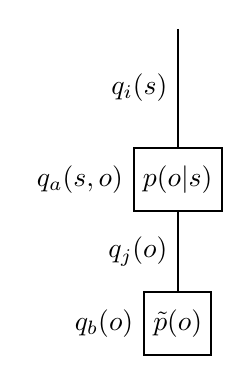
\begin{tikzpicture}[
                factor/.style={draw=black, thick, rectangle, minimum size=0.8cm, font=\normalsize},
                eqfactor/.style={draw=black, thick, rectangle, minimum size=0.5cm, font=\normalsize},
                edge/.style={thick},
                varlabel/.style={font=\normalsize},
                greycircle/.style={draw=black, thick, circle, fill=gray!30, minimum size=0.5cm, font=\normalsize}
            ]

            % Knoten
            \node[factor, label={[varlabel]left:$q_a(s,o)$}] (A1) {$p(o|s)$};
            \node[factor, below=1.0cm of A1, label={[varlabel]left:$q_b(o)$}] (c1) {$\tilde{p}(o)$};

            % Kanten zwischen Knoten
            \draw[edge] ([yshift=1.5cm]A1.north) -- (A1.north) node[midway, left, varlabel] {$q_i(s)$};
            \draw[edge] (A1.south) -- (c1.north) node[midway, left, varlabel] {$q_j(o)$};

        \end{tikzpicture}
        \caption{Perception-related factor graph sector with Bethe free energy.}
        \label{fig:32.1}
    \end{subfigure}
    \hfill
    \begin{subfigure}[t]{0.48\textwidth}
        \centering
        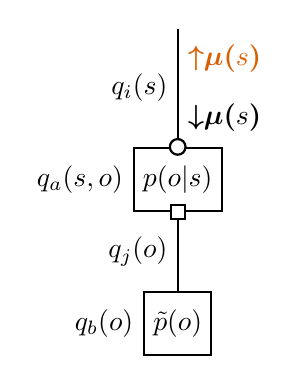
\begin{tikzpicture}[
                factor/.style={draw=black, thick, rectangle, minimum size=0.8cm, font=\normalsize},
                eqfactor/.style={draw=black, thick, rectangle, minimum size=0.5cm, font=\normalsize},
                edge/.style={thick},
                varlabel/.style={font=\normalsize},
                greycircle/.style={draw=black, thick, circle, fill=gray!30, minimum size=0.5cm, font=\normalsize}
            ]

            % Knoten
            \node[factor, label={[varlabel]left:$q_a(s,o)$}] (A1) {$p(o|s)$};
            \node[factor, below=1.0cm of A1, label={[varlabel]left:$q_b(o)$}] (c1) {$\tilde{p}(o)$};

            % Kanten zwischen Knoten
            \draw[edge] ([yshift=1.5cm]A1.north) -- (A1.north) node[midway, left, varlabel] {$q_i(s)$} node[pos=0.25, right, varlabel, scale=1.0] {$\textcolor{accorange}{\bm{{\uparrow}{\mu}(}s\bm{)}}$} node[pos=0.75, right, varlabel, scale=1.0] {$\bm{{\downarrow}{\mu}(}s\bm{)}$} node[pos=1, circle, draw=black, fill=white, inner sep=2pt] {};
            \draw[edge] (A1.south) -- (c1.north) node[midway, left, varlabel] {$q_j(o)$} node[pos=0, rectangle, draw=black, fill=white, inner sep=2.5pt] {};

        \end{tikzpicture}
        \caption{Perception-related factor graph sector with generalized free energy and corresponding GFE-based message (\(\textcolor{accorange}{\bm{{\uparrow}{\mu}(}s\bm{)}}\)).}
        \label{fig:32.2}
    \end{subfigure}
    \caption{Perception-related factor graph sectors.}
    \label{fig:32}
\end{figure}

Starting point for this derivation is the Lagrangian \(L\) of this perception-related factor graph sector with Bethe free energy (\cref{fig:32.1}) which is also used by the BFE agent:
\begin{equation}
    \begin{split}
        L = & \sum_{o,s} q_a(o,s) \ln \frac{q_a(o,s)}{p(o|s)} + \sum_o q_b(o) \ln \frac{q_b(o)}{\tilde{p}(o)} + \sum_o q_j(o) \ln \frac{1}{q_j(o)} \\
            & + \sum_s \lambda_{ia}(s) \left( q_i(s) - \sum_o q_a(o,s) \right) + \sum_o \lambda_{ja}(o) \left( q_j(o) - \sum_s q_a(o,s) \right)    \\
            & + \sum_o \lambda_{jb}(o) \left( q_j(o) - q_b(o) \right)
    \end{split}
\end{equation}
Note, that I refrain from including the normalization constraints here define following distributions via the proportional (\(\propto\)) sign.
Subtracting the entropy of \(q_i(s)\) is not necessary because it appears just once, i.e., in the local free energy of \(q_a\) (see ...).

To derive the GFE-based message there are two changes necessary in the Lagrangian \(L\). First, we add a negative mutual information term. Note, that the resulting message passing algorithm achieves a minimization of the Lagrangian which means the mutual information must have a negative sign to enable the agent to maximize the mutual information. The resulting intermediate Lagrangian \(L_{\text{MI}}\) is given in the following:
\begin{equation}
    L_{\text{MI}} = L + \sum_{o,s} q_a(o,s) \ln \frac{q_a(o)q_a(s)}{q_a(o,s)}
\end{equation}
Before applying the second change we first rearrange \(L_{\text{MI}}\) to a shorter form:
\begin{align}
    L_{\text{MI}} = & \sum_{o,s} q_a(o,s) \ln \frac{q_a(o)q_a(s)}{p(o|s)} + \sum_o q_b(o) \ln \frac{q_b(o)}{\tilde{p}(o)} + \sum_o q_j(o) \ln \frac{1}{q_j(o)} \nonumber \\
                    & + \sum_s \lambda_{ia}(s) \left( q_i(s) - \sum_o q_a(o,s) \right) + \sum_o \lambda_{ja}(o) \left( q_j(o) - \sum_s q_a(o,s) \right) \nonumber        \\
                    & + \sum_o \lambda_{jb}(o) \left( q_j(o) - q_b(o) \right)       \label{eq:37}                                                                        \\
    =               & \sum_{o,s} q_a(o,s) \ln \frac{q_a(o)q_a(s)}{p(o|s)} + \sum_o q_a(o) \ln \frac{q_a(o)}{\tilde{p}(o)} + \sum_o q_a(o) \ln \frac{1}{q_a(o)} \nonumber \\
                    & + \sum_s \lambda_{ia}(s) \left( q_i(s) - \sum_o q_a(o,s) \right) \label{eq:38}                                                                     \\
    =               & \sum_{o,s} q_a(o|s)q_a(s) \ln \frac{q_a(o)q_a(s)}{p(o|s)\tilde{p}(o)} + \sum_s \lambda_{ia}(s) \left( q_i(s) - q_a(s) \right) \label{eq:39}
\end{align}
In \cref{eq:37} I merged the local free energy of node \(a\) with the mutual information term. In \cref{eq:38} I utilized the equivalence of \(q_b(o)\), \(q_j(o)\), and \(q_a(o)\) as given by the respective marginalization constraints to substitute all \(q_b(o)\) and \(q_j(o)\) with \(q_a(o)\). In \cref{eq:39} I merged the first three terms from \cref{eq:38}, factorized \(q_a(s,o)\) in the expectation of the resulting term, and solved the sum in the remaining marginalization constraint term.

The second change consists of a "p-substitution" in which \(q_a(o|s)\) is substituted by the real likelihood \(p(o|s)\) in \cref{eq:39}. This leads to the Lagrangian \(L_{\text{GFE}}\) that entails the generalized free energy of the corresponding perception-related sector in the factor graph:
\begin{align}
    L_{\text{GFE}} = \sum_{o,s} p(o|s)q_a(s) \ln \frac{q_a(o)q_a(s)}{p(o|s)\tilde{p}(o)} + \sum_s \lambda_{ia}(s) \left( q_i(s) - q_a(s) \right)
\end{align}

The two changes to the Lagrangian are indicated in corresponding factor graph (\cref{fig:32.2}) by a small bead and a small square where the two edges terminate at node \(a\). In general, having beads at both ends of the edges means that the node local belief distribution \(q_a(o,s)\) assumes a mean-field approximation, i.e, \(q_a(o,s) = q_a(o)q_a(s)\), which is indeed the case in \(\sum_{o,s} q_a(o,s) \ln \frac{q_a(o)q_a(s)}{p(o|s)}\). Moreover, in the case when one of the variables' belief distributions (e.g., \(q_a(o)\)) is substituted by the real likelihood (i.e, \(p(o|s)\)) in the expection of the local free energy (\(\sum_{o,s} p(o|s)q_a(s) \ln \frac{q_a(o)q_a(s)}{p(o|s)}\)), then the corresponding bead of the edge that relates to this variable (edge \(j\) relates to variable \(o\)) is replaced by a rectangle.

Next, \(F_{\text{GFE}}\) is rearranged to a form that facilitates following derivations:
\begin{align}
    L_{\text{GFE}} = \sum_{o} p(o|s) \ln \frac{q_a(o)}{p(o|s)\tilde{p}(o)} + \sum_s q_a(s) \ln q_a(s) + \sum_s \lambda_{ia}(s) \left( q_i(s) - q_a(s) \right)
\end{align}

Next, the Lagrangian is differentiated with respect to \(q_a(s)\), set to \(0\), and finally solved for \(q^*_a(s)\):
\begin{alignat}{3}
     & \frac{\delta L_{\text{GFE}}}{\delta q_a(s)} &  & = \sum_{o} p(o|s) \ln \frac{q_a(o)}{p(o|s)\tilde{p}(o)} + \ln q_a(s) + 1 - \lambda_{ia}(s) \overset{!}{=} 0                                \\
     &                                             &  & \Rightarrow q^*_a(s) \propto \exp \left( \sum_{o} p(o|s) \ln \frac{p(o|s)\tilde{p}(o)}{q_a(o)} \right) \exp \left( \lambda_{ia}(s) \right)
\end{alignat}

Finally, we use the result of \cref{sec:1} for the local stationary point of \(q_i(s)\), which is:
\begin{equation}
    q^*_i(s) \propto \exp \left( \lambda_{ia}(s) \right) \exp \left( \lambda_{i\bullet}(s) \right)
\end{equation}
Here, \(\lambda_{i\bullet}\) is the Lagrange multiplier that enforces marginalization between the belief \(q_i(s)\) and the belief of the other node (besided node \(a\)) that the edge \(i\) is connected to (node not shown in \cref{fig:32}), e.g., the transition node. In the next step we will see that \(\exp \left( \lambda_{i\bullet}(s) \right)\) is the GFE-based message, i.e., the central result of this whole derivation.

To this end, we use the marginalization constraint \(q_i(s) \overset{!}{=} \sum_o q_a(o,s)\), i.e., \(q_i(s) \overset{!}{=} q_a(s)\) to relate both stationary solutions \(q^*_i(s)\) and \(q^*_a(s)\):
\begin{alignat}{2}
     & q^*_i(s)                                                                      &  & \overset{!}{=} q^*_a(s)                                                                                               \\
     & \exp \left( \lambda_{ia}(s) \right) \exp \left( \lambda_{i\bullet}(s) \right) &  & \propto \exp \left( \sum_{o} p(o|s) \ln \frac{p(o|s)\tilde{p}(o)}{q_a(o)} \right) \exp \left( \lambda_{ia}(s) \right) \\
     & \exp \left( \lambda_{i\bullet}(s) \right)                                     &  & \propto \exp \left( \sum_{o} p(o|s) \ln \frac{p(o|s)\tilde{p}(o)}{q_a(o)} \right)                                     \\
     & \textcolor{accorange}{\bm{{\uparrow}{\mu}(}s\bm{)}}                                                  &  & \propto \exp \left( \sum_{o} p(o|s) \ln \frac{p(o|s)\tilde{p}(o)}{q_a(o)} \right) \label{eq:40}
\end{alignat}

Finally, the GFE-based message that is sent by the likehood node \(a\) upwards in \cref{fig:32.2} is given in \cref{eq:40}.

Although \cref{eq:40} yields the necessary message that enables the agent to seek information in the environment, in practice the message can lead to convergence issues during inference (message passing). To accomodate for this problem we derive an alternative message that leads to a more robust message passing algorithm. In general this is achieved by developing an inference procedere that is local to the perception-related factor graph sector. During this procedere \(q_i(s)\) and \(q_j(o)\) are optimized (inferred) until convergence and only then we compute an outgoing message (analog to \(\textcolor{accorange}{\bm{{\uparrow}{\mu}(}s\bm{)}}\) in \cref{fig:32.2}) that is sent to the rest of the graph. The local inference loop consists of three recursive steps. First, we use the current (at loop step \(l-1\)) \(q^{(l-1)}_i(s)\) to compute \(q^{(l)}_j(o)\) via:
\begin{align}
    q^{(l)}_j(o) \propto \sum_s p(o|s) q^{(l-1)}_i(s) \label{eq:41}
\end{align}

Second, this result is used to compute the message from \cref{eq:40}:
\begin{align}
    \textcolor{accorange}{\bm{{\uparrow}{\mu}}^{(l)}\bm{(}s\bm{)}} \propto \exp \left( \sum_{o} p(o|s) \ln \frac{p(o|s)\tilde{p}(o)}{q_a^{(k)}(o)} \right) \label{eq:42}
\end{align}
Here, \(q_a^{(l)}(o) = q^{(l)}_j(o)\).

Third, this upward message together with the downward message \(\bm{{\downarrow}{\mu}(}s\bm{)}\) coming from the rest of the graph leads to an updated state belief:
\begin{align}
    q^{(l)}_i(s) \propto \textcolor{accorange}{\bm{{\uparrow}{\mu}}^{(l)}\bm{(}s\bm{)}} \bm{{\downarrow}{\mu}(}s\bm{)} \label{eq:43}
\end{align}

\cref{eq:41,eq:42,eq:43} are iterated until convergence of \(q_i(s)\). As a last step, the converged \(q^*_i(s)\) (signified by \(^*\)) is used to compute a final upward message (analog to \cref{eq:40}) that leads to a more stable message passing algorithm:
\begin{align}
    \textcolor{accorange}{\bm{{\uparrow}{\mu}(}s\bm{)}} \propto \frac{q^*_i(s)}{\bm{{\downarrow}{\mu}(}s\bm{)}}
\end{align}

\subsubsection{Variational Messages}

In this section I derive the variational message (\(\textcolor{accorange}{\bm{{\uparrow}{\mu}(}s\bm{)}}\)) that results from a local mean-field approximation \(q_a(o,s) = q_a(o)q_a(s)\) at the node \(a\) in \cref{fig:37.2}. This message will be sent by likelihood nodes upwards to the rest of the graph that resemble present and past timesteps of the GFE- and Context-GFE agents. In principle, also the message that is sent downwards to the observation edge will take on the same form but in this work there will always be a delta constraint (from the observation) that effectively blocks this downward message.
\begin{figure}[htbp]
    \centering
    \begin{subfigure}[t]{0.48\textwidth}
        \centering
        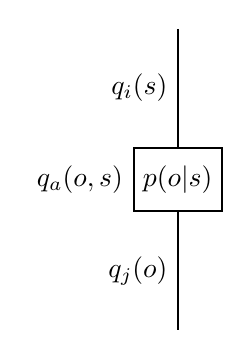
\begin{tikzpicture}[
                factor/.style={draw=black, thick, rectangle, minimum size=0.8cm, font=\normalsize},
                eqfactor/.style={draw=black, thick, rectangle, minimum size=0.5cm, font=\normalsize},
                edge/.style={thick},
                varlabel/.style={font=\normalsize},
                greycircle/.style={draw=black, thick, circle, fill=gray!30, minimum size=0.5cm, font=\normalsize}
            ]

            % Knoten
            \node[factor, label={[varlabel]left:$q_a(o,s)$}] (A1) {$p(o|s)$};

            % Kanten zwischen Knoten
            \draw[edge] ([yshift=1.5cm]A1.north) -- (A1.north) node[midway, left, varlabel] {$q_i(s)$};
            \draw[edge] (A1.south) -- ([yshift=-1.5cm]A1.south) node[midway, left, varlabel] {$q_j(o)$};

        \end{tikzpicture}
        \caption{Likelihood node with Bethe free energy.}
        \label{fig:37.1}
    \end{subfigure}
    \hfill
    \begin{subfigure}[t]{0.48\textwidth}
        \centering
        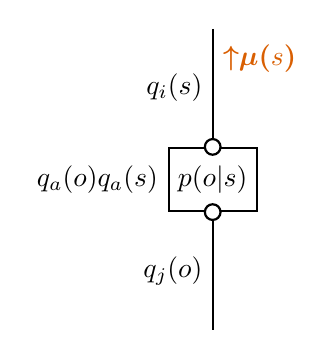
\begin{tikzpicture}[
                factor/.style={draw=black, thick, rectangle, minimum size=0.8cm, font=\normalsize},
                eqfactor/.style={draw=black, thick, rectangle, minimum size=0.5cm, font=\normalsize},
                edge/.style={thick},
                varlabel/.style={font=\normalsize},
                greycircle/.style={draw=black, thick, circle, fill=gray!30, minimum size=0.5cm, font=\normalsize}
            ]

            % Knoten
            \node[factor, label={[varlabel]left:$q_a(o)q_a(s)$}] (A1) {$p(o|s)$};

            % Kanten zwischen Knoten
            \draw[edge] ([yshift=1.5cm]A1.north) -- (A1.north) node[midway, left, varlabel] {$q_i(s)$} node[pos=0.25, right, varlabel, scale=1.0] {$\textcolor{accorange}{\bm{{\uparrow}{\mu}(}s\bm{)}}$} node[pos=1, circle, draw=black, fill=white, inner sep=2pt] {};
            \draw[edge] (A1.south) -- ([yshift=-1.5cm]A1.south) node[midway, left, varlabel] {$q_j(o)$} node[pos=0, circle, draw=black, fill=white, inner sep=2pt] {};

        \end{tikzpicture}
        \caption{Likelihood node with mean-field approximation between \(s\) and \(o\) (indicated by the two beads) and corresponding variational message (\(\textcolor{accorange}{\bm{{\uparrow}{\mu}(}s\bm{)}}\)).}
        \label{fig:37.2}
    \end{subfigure}
    \caption{Likelihood nodes for the derivation of variational messages.}
    \label{fig:37}
\end{figure}

Starting point for this derivation is the Bethe-based Lagrangian of the factor graph in \cref{fig:37.1} (excluding the marginalization constraint for \(q_j(o)\) and normalization constraints):
\begin{alignat}{2}
    L = \sum_{o,s} q_a(o,s) \ln \frac{q_a(o,s)}{p(o|s)} + \sum_s \lambda_{ia}(s) \left( q_i(s) - \sum_o q_a(o,s) \right)
\end{alignat}

Next, we introduce the mean-field approximation, i.e., \(q_a(o,s) = q_a(o)q_a(s)\), which leads to a Lagrangian that supports variational message passing (VMP):
\begin{alignat}{2}
    L_{\text{VMP}} = \sum_{o,s} q_a(o)q_a(s) \ln \frac{q_a(o)q_a(s)}{p(o|s)} + \sum_s \lambda_{ia}(s) \left( q_i(s) - \sum_o q_a(o)q_a(s) \right)
\end{alignat}

Next, we differentiate \(L_{\text{VMP}}\) with respect to \(q_a(o)\) and \(q_a(s)\), set the results to \(0\), and rearrange for \(q^*_a(o)\) and \(q^*_a(s)\):
\begin{alignat}{3}
    & \frac{\delta L_{\text{VMP}}}{\delta q_a(s)} &  & = \ln q_a(s) + 1 - \sum_o q_a(o) \ln p(o|s) - \lambda_{ia}(s) \overset{!}{=} 0                                \\
    &                                             &  & \Rightarrow q^*_a(s) \propto \exp \left( \sum_o q_a(o) \ln p(o|s) \right) \exp \left( \lambda_{ia}(s) \right)
\end{alignat}

Finally, we use the marginalization constraint (\(q_i(s) = q_a(s)\)) and the result of \cref{sec:1} for \(q_i(s)\) to derive the message \(\textcolor{accorange}{\bm{{\uparrow}{\mu}(}s\bm{)}}\):
\begin{alignat}{2}
    & q^*_i(s)                                                                      &  & \overset{!}{=} q^*_a(s)                                                                                               \\
    & \exp \left( \lambda_{ia}(s) \right) \exp \left( \lambda_{i\bullet}(s) \right) &  & \propto \exp \left( \sum_o q_a(o) \ln p(o|s) \right) \exp \left( \lambda_{ia}(s) \right) \\
    & \exp \left( \lambda_{i\bullet}(s) \right)                                     &  & \propto \exp \left( \sum_o q_a(o) \ln p(o|s) \right)         \\
    & \textcolor{accorange}{\bm{{\uparrow}{\mu}(}s\bm{)}}                                                  &  & \propto \exp \left( \sum_o q_a(o) \ln p(o|s) \right)
\end{alignat}


\subsubsection{Message Passing Algorithm}

The resulting message passing algorithm that enables the agent to perform inference is based on the whole factor graph of its temporal generative model. The factor graph is very similar to the graph from the BFE agent but additionally shows small beads and sqares at future likelihood nodes that resemble the generalized free energy which is used in these parts of the graph and leads to the information seeking behavior of the agent. Again, the graph shows an exemplary integration of an observation \(\hat{o_0}\) as a delta constraint which leads to a variational upward message there. Crucially, using GFE-based- and variational messages leads to a message passing algorithm which necessitates a recursive execution to let all belief distribution converge to a stable solution. In contrast to the algorithm of the BFE agent, this leads to an algorithm that must be run repeatedly (signified by the arrow on the left side in \cref{alg:3}). Additionally, the recursive computation of the GFE-based messages is also shown with an arrow at the left side to display the loopy execution. For this, the messages \(\textcolor{orange!75!black}{\bm{{\downarrow}{\mu}(}s^{\scriptscriptstyle II}_1\bm{)}}\), \(\textcolor{orange!75!black}{\bm{{\downarrow}{\mu}(}s_2\bm{)}}\) and beliefs \(\textcolor{accblue}{q(s^{\scriptscriptstyle II}_1)}\), \(\textcolor{accblue}{q(s_2)}\) must be initialized (e.g., uniformly) before the execution is started.

\begin{figure}[htbp]
    \centering

    \resizebox{1.0\textwidth}{!}{%
        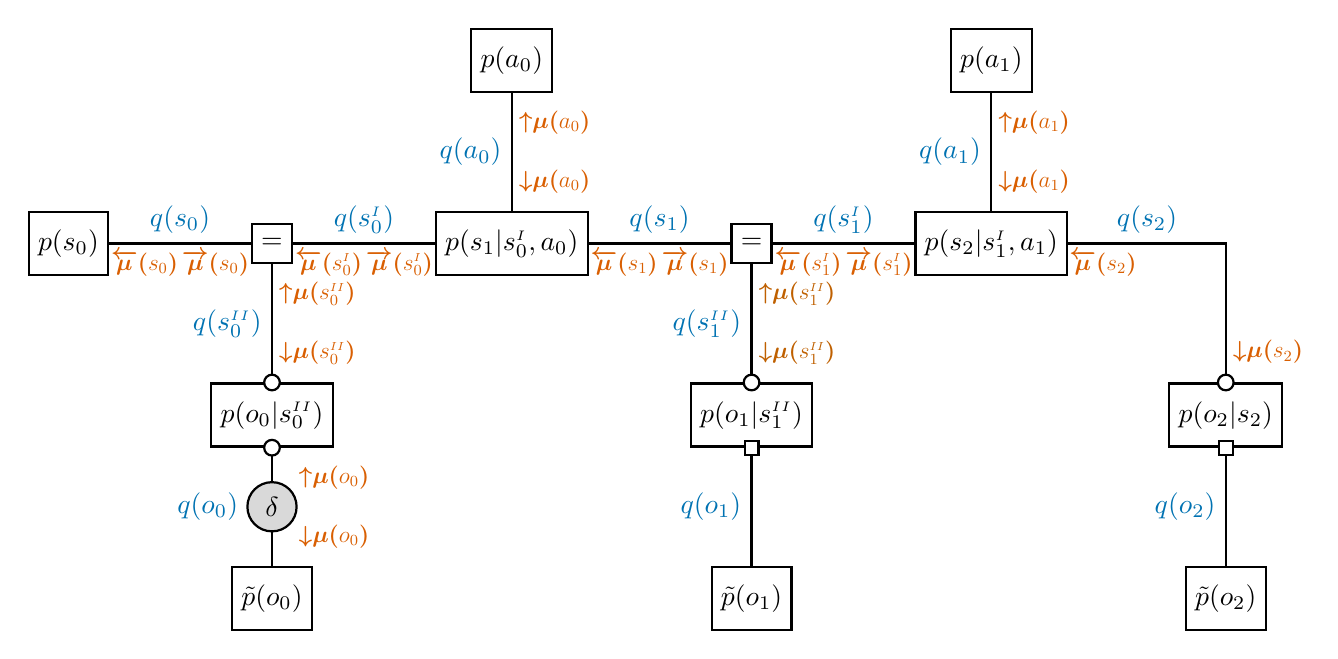
\begin{tikzpicture}[
                factor/.style={draw=black, thick, rectangle, minimum size=0.8cm, font=\normalsize},
                eqfactor/.style={draw=black, thick, rectangle, minimum size=0.5cm, font=\normalsize},
                edge/.style={thick},
                varlabel/.style={font=\normalsize},
                greycircle/.style={draw=black, thick, circle, fill=gray!30, minimum size=0.5cm, font=\normalsize}
            ]

            % Knoten
            \node[factor] (d) {$p(s_0)$};
            \node[eqfactor, right=1.8cm of d] (eq0) {$=$};
            \node[factor, below=1.5cm of eq0] (A0) {$p(o_0|s^{\scriptscriptstyle II}_0)$};
            \node[factor, below=1.5cm of A0] (c0) {$\tilde{p}(o_0)$};
            \node[factor, right=1.8cm of eq0] (B0) {$p(s_1|s^{\scriptscriptstyle I}_0,a_0)$};
            \node[eqfactor, right=1.8cm of B0] (eq1) {$=$};
            \node[factor, below=1.5cm of eq1] (A1) {$p(o_1|s^{\scriptscriptstyle II}_1)$};
            \node[factor, below=1.5cm of A1] (c1) {$\tilde{p}(o_1)$};
            \node[factor, right=1.8cm of eq1] (B1) {$p(s_2|s^{\scriptscriptstyle I}_1,a_1)$};
            \node[factor] (A2) at ([xshift=2cm] B1.east |- A1) {$p(o_2|s_2)$};
            \node[factor, below=1.5cm of A2] (c2) {$\tilde{p}(o_2)$};
            \node[factor, above=1.5cm of B0] (u0) {$p(a_0)$};
            \node[factor, above=1.5cm of B1] (u1) {$p(a_1)$};

            % Kanten zwischen Knoten
            \draw[edge] (d.east) -- (eq0.west) node[midway, above, varlabel] {$\textcolor{accblue}{q(s_0)}$} node[near end, below, varlabel, scale=0.7] {${\large \textcolor{accorange}{\bm{\overrightarrow{\mu}(}s_0\bm{)}}}$} node[near start, below, varlabel, scale=0.7] {${\large \textcolor{accorange}{\bm{\overleftarrow{\mu}(}s_0\bm{)}}}$};
            \draw[edge] (eq0.south) -- (A0.north) node[midway, left, varlabel] {$\textcolor{accblue}{q(s^{\scriptscriptstyle II}_0)}$} node[pos=0.25, right, varlabel, scale=0.7] {${\large \textcolor{accorange}{\bm{{\uparrow}{\mu}(}s^{\scriptscriptstyle II}_0\bm{)}}}$} node[pos=0.75, right, varlabel, scale=0.7] {${\large \textcolor{accorange}{\bm{{\downarrow}{\mu}(}s^{\scriptscriptstyle II}_0\bm{)}}}$}  node[pos=1, circle, draw=black, fill=white, inner sep=2pt] {};
            \draw[edge] (A0.south) -- (c0.north) node[midway, greycircle] {$\delta$} node[midway, left=0.3, varlabel] {$\textcolor{accblue}{q(o_0)}$} node[pos=0.25, right=0.25, varlabel, scale=0.7] {${\large \textcolor{accorange}{\bm{{\uparrow}{\mu}(}o_0\bm{)}}}$} node[pos=0.75, right=0.25, varlabel, scale=0.7] {${\large \textcolor{accorange}{\bm{{\downarrow}{\mu}(}o_0\bm{)}}}$}  node[pos=0, circle, draw=black, fill=white, inner sep=2pt] {};
            \draw[edge] (eq0.east) -- (B0.west) node[midway, above, varlabel] {$\textcolor{accblue}{q(s^{\scriptscriptstyle I}_0)}$} node[near start, below, varlabel, scale=0.7] {${\large \textcolor{accorange}{\bm{\overleftarrow{\mu}(}s^{\scriptscriptstyle I}_0\bm{)}}}$} node[near end, below, varlabel, scale=0.7] {${\large \textcolor{accorange}{\bm{\overrightarrow{\mu}(}s^{\scriptscriptstyle I}_0\bm{)}}}$};
            \draw[edge] (B0.north) -- (u0.south) node[midway, left, varlabel] {$\textcolor{accblue}{q(a_0)}$} node[pos=0.25, right, varlabel, scale=0.7] {${\large \textcolor{accorange}{\bm{{\downarrow}{\mu}(}a_0\bm{)}}}$} node[pos=0.75, right, varlabel, scale=0.7] {${\large \textcolor{accorange}{\bm{{\uparrow}{\mu}(}a_0\bm{)}}}$};
            \draw[edge] (B0.east) -- (eq1.west) node[midway, above, varlabel] {$\textcolor{accblue}{q(s_1)}$} node[near end, below, varlabel, scale=0.7] {${\large \textcolor{accorange}{\bm{\overrightarrow{\mu}(}s_1\bm{)}}}$} node[near start, below, varlabel, scale=0.7] {${\large \textcolor{accorange}{\bm{\overleftarrow{\mu}(}s_1\bm{)}}}$};
            \draw[edge] (eq1.south) -- (A1.north) node[midway, left, varlabel] {$\textcolor{accblue}{q(s^{\scriptscriptstyle II}_1)}$} node[pos=0.25, right, varlabel, scale=0.7] {${\large \textcolor{orange!75!black}{\bm{{\uparrow}{\mu}(}s^{\scriptscriptstyle II}_1\bm{)}}}$} node[pos=0.75, right, varlabel, scale=0.7] {${\large \textcolor{orange!75!black}{\bm{{\downarrow}{\mu}(}s^{\scriptscriptstyle II}_1\bm{)}}}$} node[pos=1, circle, draw=black, fill=white, inner sep=2pt] {};
            \draw[edge] (A1.south) -- (c1.north) node[midway, left, varlabel] {$\textcolor{accblue}{q(o_1)}$} node[pos=0, rectangle, draw=black, fill=white, inner sep=2.5pt] {};
            \draw[edge] (eq1.east) -- (B1.west) node[midway, above, varlabel] {$\textcolor{accblue}{q(s^{\scriptscriptstyle I}_1)}$} node[near start, below, varlabel, scale=0.7] {${\large \textcolor{accorange}{\bm{\overleftarrow{\mu}(}s^{\scriptscriptstyle I}_1\bm{)}}}$} node[near end, below, varlabel, scale=0.7] {${\large \textcolor{accorange}{\bm{\overrightarrow{\mu}(}s^{\scriptscriptstyle I}_1\bm{)}}}$};
            \draw[edge] (B1.east) -| (A2.north) node[pos=0.25, above, varlabel] {$\textcolor{accblue}{q(s_2)}$} node[pos=0.89, right, varlabel, scale=0.7] {${\large \textcolor{accorange}{\bm{{\downarrow}{\mu}(}s_2\bm{)}}}$} node[pos=0.11, below, varlabel, scale=0.7] {${\large \textcolor{accorange}{\bm{\overleftarrow{\mu}(}s_2\bm{)}}}$} node[pos=1, circle, draw=black, fill=white, inner sep=2pt] {};
            \draw[edge] (A2.south) -- (c2.north) node[midway, left, varlabel] {$\textcolor{accblue}{q(o_2)}$} node[pos=0, rectangle, draw=black, fill=white, inner sep=2.5pt] {};
            \draw[edge] (B1.north) -- (u1.south) node[midway, left, varlabel] {$\textcolor{accblue}{q(a_1)}$} node[pos=0.25, right, varlabel, scale=0.7] {${\large \textcolor{accorange}{\bm{{\downarrow}{\mu}(}a_1\bm{)}}}$} node[pos=0.75, right, varlabel, scale=0.7] {${\large \textcolor{accorange}{\bm{{\uparrow}{\mu}(}a_1\bm{)}}}$};

        \end{tikzpicture}
    }

    \caption{Factor graph of the GFE agent with variables' belief distributions \(\textcolor{accblue}{q}\) and messages \(\textcolor{accorange}{\mu}\).}
    \label{fig:33}
\end{figure}

\begin{algorithm}[htbp]
    \caption{Message Passing Algorithm of the GFE Agent}
    \label{alg:3}
    \small
    \begin{algorithmic}[1] % Die [1] sorgt für automatische Zeilennummern!
        \linespread{1.4}\selectfont
        \setlength{\leftskip}{0.3cm}
        \State \tikzmark{algtop3}$\textcolor{accorange}{\bm{\overrightarrow{\mu}(}s_0\bm{)}} \propto p(s_0)$,\quad$\textcolor{accorange}{\bm{{\uparrow}{\mu}(}o_0\bm{)}} \propto \delta_{o_0,\hat{o_0}}$,\quad$\textcolor{accorange}{\bm{{\downarrow}{\mu}(}a_0\bm{)}} \propto p(a_0)$,\quad$\textcolor{accorange}{\bm{{\downarrow}{\mu}(}a_1\bm{)}} \propto p(a_1)$,\quad$\textcolor{accorange}{\bm{{\downarrow}{\mu}(}o_0\bm{)}} \propto \delta_{o_0,\hat{o_0}}$
        \State $\textcolor{accorange}{\bm{{\uparrow}{\mu}(}s^{\scriptscriptstyle II}_0\bm{)}} \propto \exp \left( \sum_{o_0} q(o_0) p(o_0|s^{\scriptscriptstyle II}_0) \right)$,
        \Statex \quad\quad\tikzmark{onetop3}$q^{(l)}(o_1) \propto \sum_{s^{\scriptscriptstyle II}_1} p(o_1|s^{\scriptscriptstyle II}_1) q^{(l-1)}(s^{\scriptscriptstyle II}_1)$
        \Statex \quad\quad$\bm{{\uparrow}{\mu}}^{(l)}\bm{(}s^{\scriptscriptstyle II}_1\bm{)} \propto \exp \left( \sum_{o_1} p(o_1|s^{\scriptscriptstyle II}_1) \ln \frac{p(o_1|s^{\scriptscriptstyle II}_1)\tilde{p}(o_1)}{q^{(l)}(o_1)} \right)$
        \Statex \quad\quad\tikzmark{onebottom3}$q^{(l)}(s^{\scriptscriptstyle II}_1) \propto \bm{{\uparrow}{\mu}}^{(l)}\bm{(}s^{\scriptscriptstyle II}_1\bm{)} \bm{{\downarrow}{\mu}(}s^{\scriptscriptstyle II}_1\bm{)}$
        \Statex $\textcolor{accorange}{\bm{{\uparrow}{\mu}(}s^{\scriptscriptstyle II}_1\bm{)}} \propto \frac{q^*(s^{\scriptscriptstyle II}_1)}{\bm{{\downarrow}{\mu}(}s^{\scriptscriptstyle II}_1\bm{)}}$,
        \Statex \quad\quad\tikzmark{twotop3}$q^{(l)}(o_2) \propto \sum_{s_2} p(o_2|s_2) q^{(l-1)}(s_2)$
        \Statex \quad\quad$\bm{{\uparrow}{\mu}}^{(l)}\bm{(}s_2\bm{)} \propto \exp \left( \sum_{o_2} p(o_2|s_2) \ln \frac{p(o_2|s_2)\tilde{p}(o_2)}{q^{(l)}(o_2)} \right)$
        \Statex \quad\quad\tikzmark{twobottom3}$q^{(l)}(s_2) \propto \bm{{\uparrow}{\mu}}^{(l)}\bm{(}s_2\bm{)} \bm{{\downarrow}{\mu}(}s_2\bm{)}$
        \Statex $\textcolor{accorange}{\bm{\overleftarrow{\mu}(}s_2\bm{)}} \propto \frac{q^*(s_2)}{\bm{{\downarrow}{\mu}(}s_2\bm{)}}$
        \State $\textcolor{accorange}{\bm{\overrightarrow{\mu}(}s^{\scriptscriptstyle I}_0\bm{)}} \propto \sum_{s_0,s^{\scriptscriptstyle II}_0} \delta_{s_0,s^{\scriptscriptstyle I}_0}\delta_{s_0,s^{\scriptscriptstyle II}_0} \textcolor{black}{\bm{\overrightarrow{\mu}(}s_0\bm{)}} \textcolor{black}{\bm{{\uparrow}{\mu}(}s^{\scriptscriptstyle II}_0\bm{)}}$,\quad$\textcolor{accorange}{\bm{\overleftarrow{\mu}(}s^{\scriptscriptstyle I}_1\bm{)}} \propto \sum_{a_1,s_2} p(s_2|s^{\scriptscriptstyle I}_1,a_1) \textcolor{black}{\bm{{\downarrow}{\mu}(}a_1\bm{)}} \textcolor{black}{\bm{\overleftarrow{\mu}(}s_2\bm{)}}$,
        \State $\textcolor{accorange}{\bm{\overrightarrow{\mu}(}s_1\bm{)}} \propto \sum_{s^{\scriptscriptstyle I}_0,a_0} p(s_1|s^{\scriptscriptstyle I}_0,a_0) \textcolor{black}{\bm{\overrightarrow{\mu}(}s^{\scriptscriptstyle I}_0\bm{)}} \textcolor{black}{\bm{{\downarrow}{\mu}(}a_0\bm{)}}$,\quad$\textcolor{accorange}{\bm{\overleftarrow{\mu}(}s_1\bm{)}} \propto \sum_{s^{\scriptscriptstyle I}_1,s^{\scriptscriptstyle II}_1} \delta_{s_1,s^{\scriptscriptstyle I}_1}\delta_{s_1,s^{\scriptscriptstyle II}_1} \textcolor{black}{\bm{\overleftarrow{\mu}(}s^{\scriptscriptstyle I}_1\bm{)}} \textcolor{black}{\bm{{\uparrow}{\mu}(}s^{\scriptscriptstyle II}_1\bm{)}}$
        \State $\textcolor{accorange}{\bm{\overrightarrow{\mu}(}s^{\scriptscriptstyle I}_1\bm{)}} \propto \sum_{s_1,s^{\scriptscriptstyle II}_1} \delta_{s_1,s^{\scriptscriptstyle I}_1}\delta_{s_1,s^{\scriptscriptstyle II}_1} \textcolor{black}{\bm{\overrightarrow{\mu}(}s_1\bm{)}} \textcolor{black}{\bm{{\uparrow}{\mu}(}s^{\scriptscriptstyle II}_1\bm{)}}$,\quad$\textcolor{accorange}{\bm{{\downarrow}{\mu}(}s^{\scriptscriptstyle II}_1\bm{)}} \propto \sum_{s_1,s^{\scriptscriptstyle I}_1} \delta_{s_1,s^{\scriptscriptstyle I}_1}\delta_{s_1,s^{\scriptscriptstyle II}_1} \textcolor{black}{\bm{\overrightarrow{\mu}(}s_1\bm{)}} \textcolor{black}{\bm{\overleftarrow{\mu}(}s^{\scriptscriptstyle I}_1\bm{)}}$,
        \Statex $\textcolor{accorange}{\bm{{\uparrow}{\mu}(}a_0\bm{)}} \propto \sum_{s_1,s^{\scriptscriptstyle I}_0} p(s_1|s^{\scriptscriptstyle I}_0,a_0) \textcolor{black}{\bm{\overrightarrow{\mu}(}s^{\scriptscriptstyle I}_0\bm{)}} \textcolor{black}{\bm{\overleftarrow{\mu}(}s_1\bm{)}}$,\quad$\textcolor{accorange}{\bm{\overleftarrow{\mu}(}s^{\scriptscriptstyle I}_0\bm{)}} \propto \sum_{s_1,a_0} p(s_1|s^{\scriptscriptstyle I}_0,a_0) \textcolor{black}{\bm{{\downarrow}{\mu}(}a_0\bm{)}} \textcolor{black}{\bm{\overleftarrow{\mu}(}s_1\bm{)}}$
        \State $\textcolor{accorange}{\bm{{\uparrow}{\mu}(}a_1\bm{)}} \propto \sum_{s^{\scriptscriptstyle I}_1,s_2} p(s_2|s^{\scriptscriptstyle I}_1,a_1) \textcolor{black}{\bm{\overrightarrow{\mu}(}s^{\scriptscriptstyle I}_1\bm{)}} \textcolor{black}{\bm{\overleftarrow{\mu}(}s_2\bm{)}}$,\quad$\textcolor{accorange}{\bm{{\downarrow}{\mu}(}s_2\bm{)}} \propto \sum_{s^{\scriptscriptstyle I}_1,a_1} p(s_2|s^{\scriptscriptstyle I}_1,a_1) \textcolor{black}{\bm{\overrightarrow{\mu}(}s^{\scriptscriptstyle I}_1\bm{)}} \textcolor{black}{\bm{{\downarrow}{\mu}(}a_1\bm{)}}$,
        \Statex $\textcolor{accorange}{\bm{\overleftarrow{\mu}(}s_0\bm{)}} \propto \sum_{s^{\scriptscriptstyle I}_0,s^{\scriptscriptstyle II}_0} \delta_{s_0,s^{\scriptscriptstyle I}_0}\delta_{s_0,s^{\scriptscriptstyle II}_0} \textcolor{black}{\bm{\overleftarrow{\mu}(}s^{\scriptscriptstyle I}_0\bm{)}} \textcolor{black}{\bm{{\uparrow}{\mu}(}s^{\scriptscriptstyle II}_0\bm{)}}$,\quad$\textcolor{accorange}{\bm{{\downarrow}{\mu}(}s^{\scriptscriptstyle II}_0\bm{)}} \propto \sum_{s_0,s^{\scriptscriptstyle I}_0} \delta_{s_0,s^{\scriptscriptstyle I}_0}\delta_{s_0,s^{\scriptscriptstyle II}_0} \textcolor{black}{\bm{\overrightarrow{\mu}(}s_0\bm{)}} \textcolor{black}{\bm{\overleftarrow{\mu}(}s^{\scriptscriptstyle I}_0\bm{)}}$
        \State \tikzmark{algbottom3}$\textcolor{accblue}{q(s_0)} \propto \textcolor{black}{\bm{\overleftarrow{\mu}(}s_0\bm{)}} \textcolor{black}{\bm{\overrightarrow{\mu}(}s_0\bm{)}}$,\quad$\textcolor{accblue}{q(s^{\scriptscriptstyle I}_0)} \propto \textcolor{black}{\bm{\overleftarrow{\mu}(}s^{\scriptscriptstyle I}_0\bm{)}} \textcolor{black}{\bm{\overrightarrow{\mu}(}s^{\scriptscriptstyle I}_0\bm{)}}$,\quad$\textcolor{accblue}{q(s^{\scriptscriptstyle II}_0)} \propto \textcolor{black}{\bm{{\uparrow}{\mu}(}s^{\scriptscriptstyle II}_0\bm{)}} \textcolor{black}{\bm{{\downarrow}{\mu}(}s^{\scriptscriptstyle II}_0\bm{)}}$,
        \Statex $\textcolor{accblue}{q(s_1)} \propto \textcolor{black}{\bm{\overleftarrow{\mu}(}s_1\bm{)}} \textcolor{black}{\bm{\overrightarrow{\mu}(}s_1\bm{)}}$,\quad$\textcolor{accblue}{q(s^{\scriptscriptstyle I}_1)} \propto \textcolor{black}{\bm{\overleftarrow{\mu}(}s^{\scriptscriptstyle I}_1\bm{)}} \textcolor{black}{\bm{\overrightarrow{\mu}(}s^{\scriptscriptstyle I}_1\bm{)}}$,\quad$\textcolor{accblue}{q(s^{\scriptscriptstyle II}_1)} \propto \textcolor{black}{\bm{{\uparrow}{\mu}(}s^{\scriptscriptstyle II}_1\bm{)}} \textcolor{black}{\bm{{\downarrow}{\mu}(}s^{\scriptscriptstyle II}_1\bm{)}}$,
        \Statex $\textcolor{accblue}{q(s_2)} \propto \textcolor{black}{\bm{\overleftarrow{\mu}(}s_2\bm{)}} \textcolor{black}{\bm{{\downarrow}{\mu}(}s_2\bm{)}}$,\quad$\textcolor{accblue}{q(a_0)} \propto \textcolor{black}{\bm{{\uparrow}{\mu}(}a_0\bm{)}} \textcolor{black}{\bm{{\downarrow}{\mu}(}a_0\bm{)}}$,\quad$\textcolor{accblue}{q(a_1)} \propto \textcolor{black}{\bm{{\uparrow}{\mu}(}a_1\bm{)}} \textcolor{black}{\bm{{\downarrow}{\mu}(}a_1\bm{)}}$,
        \Statex $\textcolor{accblue}{q(o_0)} \propto \textcolor{black}{\bm{{\uparrow}{\mu}(}o_0\bm{)}} \textcolor{black}{\bm{{\downarrow}{\mu}(}o_0\bm{)}}$,\quad$\textcolor{accblue}{q(o_1)} \propto \sum_{s^{\scriptscriptstyle II}_1} p(o_1|s^{\scriptscriptstyle II}_1) q(s^{\scriptscriptstyle II}_1)$,\quad$\textcolor{accblue}{q(o_2)} \propto \sum_{s_2} p(o_2|s_2) q(s_2)$
    \end{algorithmic}

    \begin{tikzpicture}[remember picture, overlay]
        \draw[-{Stealth[length=2.2mm, width=1.6mm]}, thick, gray!75!black, rounded corners=5pt]
        ([yshift=0.5ex, xshift=-2.5ex]pic cs:algbottom3) -- ++(-0.4cm, 0) |- ([xshift=-2.5ex, yshift=0.5ex]pic cs:algtop3);
    \end{tikzpicture}
    \begin{tikzpicture}[remember picture, overlay]
        \draw[-{Stealth[length=2.2mm, width=1.6mm]}, thick, gray!75!black, rounded corners=5pt]
        ([yshift=0.5ex, xshift=-0.5ex]pic cs:onebottom3) -- ++(-0.4cm, 0) |- ([xshift=-0.5ex, yshift=0.5ex]pic cs:onetop3);
    \end{tikzpicture}
    \begin{tikzpicture}[remember picture, overlay]
        \draw[-{Stealth[length=2.2mm, width=1.6mm]}, thick, gray!75!black, rounded corners=5pt]
        ([yshift=0.5ex, xshift=-0.5ex]pic cs:twobottom3) -- ++(-0.4cm, 0) |- ([xshift=-0.5ex, yshift=0.5ex]pic cs:twotop3);
    \end{tikzpicture}

\end{algorithm}


\subsection{Context-BFE Agent}
\label{sec:context-bfe}

The Context-BFE agent is similar to the BFE agent but entails another hidden context state as part of its generative model. Specifically, the agent does not only assume that observations are generated by hidden states \(s\) but additionaly assumes a hidden context state \(c\) that also influences observations. In contrast to states \(s\), the context state does not change for each timestep and thus is assumed to be persistent during multiple timesteps. In later simulations, there will only be a single context state during the succession of three regular hidden states \(s\). The corresponding POMDP is given by
\begin{equation}
    \begin{split}
        p(o_0, o_1, o_2, s_0, s_1, s_2, c, a_0, a_1) = \; & \tilde{p}(o_0) p(o_0|s_0,c) p(s_0) p(c)           \\
                                                          & \tilde{p}(o_1) p(o_1|s_1,c) p(s_1|s_0,a_0) p(a_0) \\
                                                          & \tilde{p}(o_2) p(o_2|s_2,c) p(s_2|s_1,a_1) p(a_1)
        \label{eq:35}
    \end{split}
\end{equation}
and entails a prior over the context \(p(c)\) similarly to the initial prior over the hidden state \(p(s_0)\). The corresponding factor graph of \cref{eq:35} is given in \cref{fig:28}.

\begin{figure}[htbp]
    \centering

    \resizebox{1.0\textwidth}{!}{%
        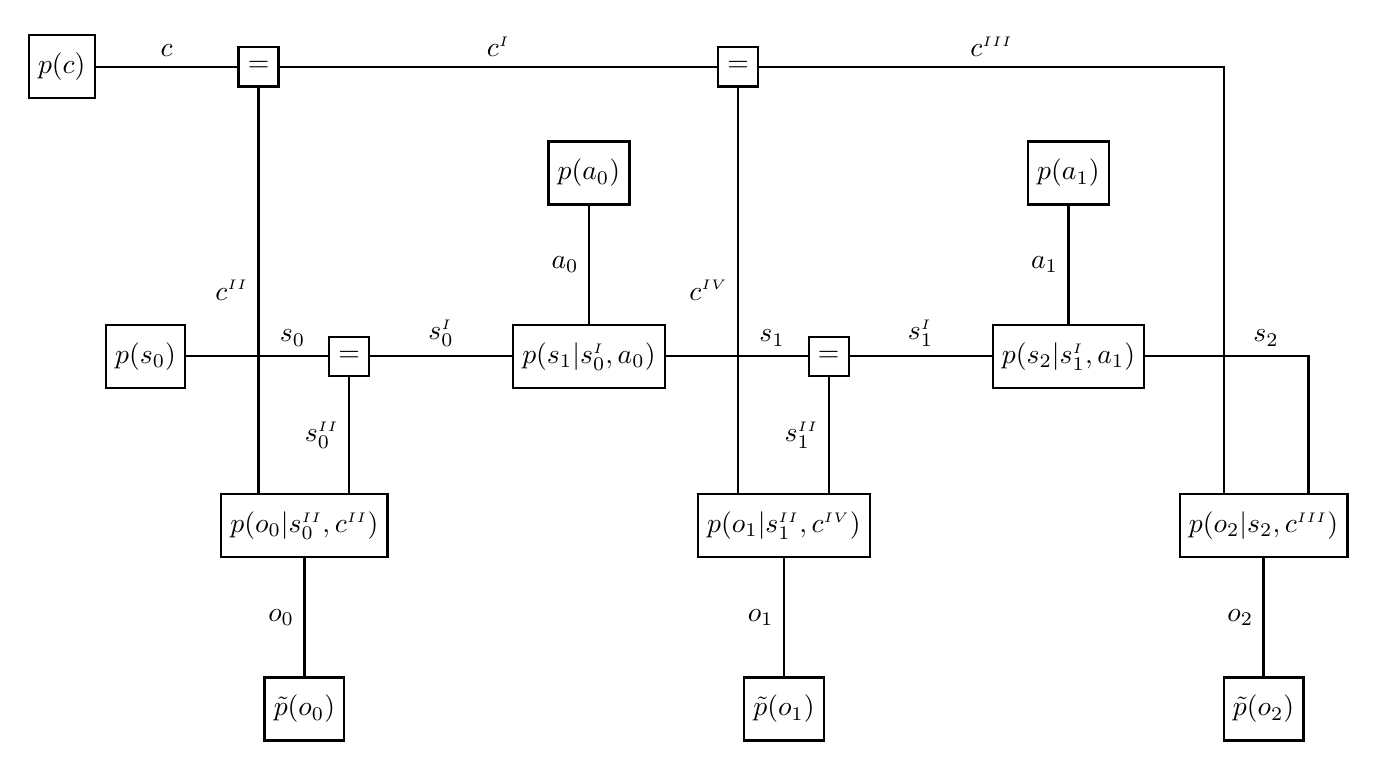
\begin{tikzpicture}[
                factor/.style={draw=black, thick, rectangle, minimum size=0.8cm, font=\normalsize},
                eqfactor/.style={draw=black, thick, rectangle, minimum size=0.5cm, font=\normalsize},
                edge/.style={thick},
                varlabel/.style={font=\normalsize},
                greycircle/.style={draw=black, thick, circle, fill=gray!30, minimum size=0.5cm, font=\normalsize}
            ]

            % Knoten
            \node[factor] (d) {$p(s_0)$};
            \node[eqfactor, right=1.8cm of d] (eq0) {$=$};
            \node[factor] (A0) at ([xshift=1.5cm, yshift=-2.15cm] d.east) {$p(o_0|s^{\scriptscriptstyle II}_0,c^{\scriptscriptstyle II})$};
            \node[factor, below=1.5cm of A0] (c0) {$\tilde{p}(o_0)$};
            \node[factor, right=1.8cm of eq0] (B0) {$p(s_1|s^{\scriptscriptstyle I}_0,a_0)$};
            \node[eqfactor, right=1.8cm of B0] (eq1) {$=$};
            \node[factor] (A1) at ([xshift=1.5cm, yshift=-2.15cm] B0.east) {$p(o_1|s^{\scriptscriptstyle II}_1,c^{\scriptscriptstyle IV})$};
            \node[factor, below=1.5cm of A1] (c1) {$\tilde{p}(o_1)$};
            \node[factor, right=1.8cm of eq1] (B1) {$p(s_2|s^{\scriptscriptstyle I}_1,a_1)$};
            \node[factor] (A2) at ([xshift=1.5cm] B1.east |- A1) {$p(o_2|s_2,c^{\scriptscriptstyle III})$};
            \node[factor, below=1.5cm of A2] (c2) {$\tilde{p}(o_2)$};
            \node[factor, above=1.5cm of B0] (u0) {$p(a_0)$};
            \node[factor, above=1.5cm of B1] (u1) {$p(a_1)$};
            \node[eqfactor, above right=3cm and 0.65cm of d] (eq3) {$=$};
            \node[eqfactor, above right=3cm and 0.65cm of B0] (eq4) {$=$};
            \node[factor, left=1.8cm of eq3] (dc) {$p(c)$};

            % Kanten zwischen Knoten
            \draw[edge] (d.east) -- (eq0.west) node[pos=0.75, above, varlabel] {$s_0$};
            \draw[edge] (eq0.south) -- (eq0.south |- A0.north) node[midway, left, varlabel] {$s^{\scriptscriptstyle II}_0$};
            \draw[edge] (A0.south) -- (c0.north) node[midway, left, varlabel] {$o_0$};
            \draw[edge] (eq0.east) -- (B0.west) node[midway, above, varlabel] {$s^{\scriptscriptstyle I}_0$};
            \draw[edge] (B0.north) -- (u0.south) node[midway, left, varlabel] {$a_0$};
            \draw[edge] (B0.east) -- (eq1.west) node[pos=0.75, above, varlabel] {$s_1$};
            \draw[edge] (eq1.south) -- (eq1.south |- A1.north) node[midway, left, varlabel] {$s^{\scriptscriptstyle II}_1$};
            \draw[edge] (A1.south) -- (c1.north) node[midway, left, varlabel] {$o_1$};
            \draw[edge] (eq1.east) -- (B1.west) node[midway, above, varlabel] {$s^{\scriptscriptstyle I}_1$};
            \draw[edge] (B1.east) -| ([xshift=0.57cm]A2.north) node[pos=0.37, above, varlabel] {$s_2$};
            \draw[edge] (A2.south) -- (c2.north) node[midway, left, varlabel] {$o_2$};
            \draw[edge] (B1.north) -- (u1.south) node[midway, left, varlabel] {$a_1$};
            \draw[edge] (dc.east) -- (eq3.west) node[midway, above, varlabel] {$c$};
            \draw[edge] (eq3.east) -- (eq4.west) node[midway, above, varlabel] {$c^{\scriptscriptstyle I}$};
            \draw[edge] (eq4.east) -| ([xshift=-0.5cm]A2.north) node[pos=0.25, above, varlabel] {$c^{\scriptscriptstyle III}$};
            \draw[edge] (eq3.south) -- (eq3.south |- A0.north) node[midway, left, varlabel] {$c^{\scriptscriptstyle II}$};
            \draw[edge] (eq4.south) -- (eq4.south |- A1.north) node[midway, left, varlabel] {$c^{\scriptscriptstyle IV}$};

        \end{tikzpicture}
    }
    \caption{Foundational Factor Graph of the two Context Agents.}
    \label{fig:28}
\end{figure}

In principle, the derivation of messages based on the factor graph's Bethe free energy is straightforward (compare \cref{sec:1}). In practice, the addition of a hidden context state leads to factor graph that contains loops (e.g., \(c^{\scriptscriptstyle II}_0 \rightarrow c^{\scriptscriptstyle I}_0 \rightarrow c^{\scriptscriptstyle IV}_0 \rightarrow s^{\scriptscriptstyle II}_1 \rightarrow s_1 \rightarrow s^{\scriptscriptstyle I}_0 \rightarrow s^{\scriptscriptstyle II}_0 \rightarrow c^{\scriptscriptstyle II}_0\)). Given this situation, messages derived from the Bethe free energy might lead to a message passing algorithm which might not yield stable solutions for the belief distributions, i.e, the algorithm might not converge. The problem lies at the nodes' belief distributions that explicitly respect dependencies between variables of the node, e.g., the belief distribution \(q(o_0,s^{\scriptscriptstyle II}_0,c^{\scriptscriptstyle II}_0)\) at the node \(p(o_0|s^{\scriptscriptstyle II}_0,c^{\scriptscriptstyle II}_0)\) respects the dependencies between the variables \(o_0\), \(s^{\scriptscriptstyle II}_0\), and \(c^{\scriptscriptstyle II}_0\). The solution to the convergence issues of pure Bethe free energy related message passing algorithm in graphs with loops lies in breaking up these dependencies to break the loop. Following this, it is then sufficient to define this node's belief distribution as \(q(o_0,s^{\scriptscriptstyle II}_0,c^{\scriptscriptstyle II}_0) = q(o_0,s^{\scriptscriptstyle II}_0)q(c^{\scriptscriptstyle II}_0)\). In this way, the dependencies between \(c^{\scriptscriptstyle II}_0\) and the other two variables are broken up in the belief distribution which eventually breaks the prior exemplary loop and the resulting message passing algorithm yields stable solutions, i.e., it converges. Breaking up these dependencies in nodes' belief distributions leads to structured variational messages that are sent from the respective nodes. These messages are derived in the following section.

\subsubsection{Structured Variational Messages}

Starting point for this derivation is a factor node with three edges (\cref{fig:34.1}), i.e, three variables.

\begin{figure}[htbp]
    \centering
    \begin{subfigure}[t]{0.48\textwidth}
        \centering
        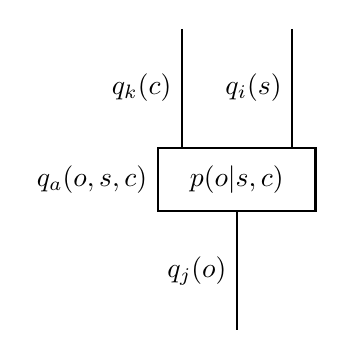
\begin{tikzpicture}[
                factor/.style={draw=black, thick, rectangle, minimum size=0.8cm, minimum width=2.0cm, font=\normalsize},
                eqfactor/.style={draw=black, thick, rectangle, minimum size=0.5cm, font=\normalsize},
                edge/.style={thick},
                varlabel/.style={font=\normalsize},
                greycircle/.style={draw=black, thick, circle, fill=gray!30, minimum size=0.5cm, font=\normalsize}
            ]

            % Knoten
            \node[factor, label={[varlabel]left:$q_a(o,s,c)$}] (A1) {$p(o|s,c)$};

            % Kanten zwischen Knoten
            \draw[edge] ([yshift=1.5cm,xshift=0.7cm]A1.north) -- ([xshift=0.7cm]A1.north) node[midway, left, varlabel] {$q_i(s)$};
            \draw[edge] (A1.south) -- ([yshift=-1.5cm]A1.south) node[midway, left, varlabel] {$q_j(o)$};
            \draw[edge] ([yshift=1.5cm,xshift=-0.7cm]A1.north) -- ([xshift=-0.7cm]A1.north) node[midway, left, varlabel] {$q_k(c)$};

        \end{tikzpicture}
        \caption{Factor node with node belief that respects variables' dependencies.}
        \label{fig:34.1}
    \end{subfigure}
    \hfill
    \begin{subfigure}[t]{0.48\textwidth}
        \centering
        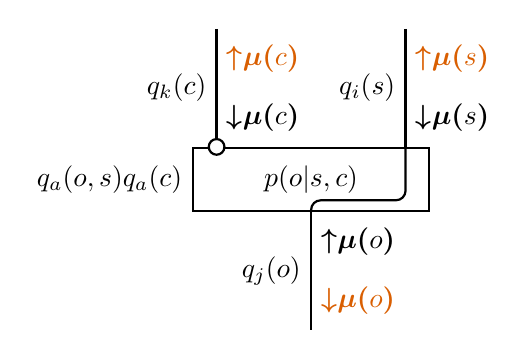
\begin{tikzpicture}[
                factor/.style={draw=black, thick, rectangle, minimum size=0.8cm, minimum width=3.0cm, font=\normalsize},
                eqfactor/.style={draw=black, thick, rectangle, minimum size=0.5cm, font=\normalsize},
                edge/.style={thick},
                varlabel/.style={font=\normalsize},
                greycircle/.style={draw=black, thick, circle, fill=gray!30, minimum size=0.5cm, font=\normalsize}
            ]

            % Knoten
            \node[factor, label={[varlabel]left:$q_a(o,s)q_a(c)$}] (A1) {$p(o|s,c)$};

            % Kanten zwischen Knoten
            \draw[edge] ([yshift=1.5cm,xshift=1.2cm]A1.north) -- ([xshift=1.2cm]A1.north) node[midway, left, varlabel] {$q_i(s)$} node[pos=0.25, right, varlabel] {$\textcolor{accorange}{\bm{{\uparrow}{\mu}(}s\bm{)}}$} node[pos=0.75, right, varlabel] {$\bm{{\downarrow}{\mu}(}s\bm{)}$} {};
            \draw[edge] (A1.south) -- ([yshift=-1.5cm]A1.south) node[midway, left, varlabel] {$q_j(o)$} node[pos=0.25, right, varlabel] {$\bm{{\uparrow}{\mu}(}o\bm{)}$} node[pos=0.75, right, varlabel] {$\textcolor{accorange}{\bm{{\downarrow}{\mu}(}o\bm{)}}$} {};
            \draw[edge] ([yshift=1.5cm,xshift=-1.2cm]A1.north) -- ([xshift=-1.2cm]A1.north) node[midway, left, varlabel] {$q_k(c)$} node[pos=0.25, right, varlabel] {$\textcolor{accorange}{\bm{{\uparrow}{\mu}(}c\bm{)}}$} node[pos=0.75, right, varlabel] {$\bm{{\downarrow}{\mu}(}c\bm{)}$} node[pos=1, circle, draw=black, fill=white, inner sep=2pt] {};
            \draw[edge, rounded corners=3.5pt]
            ([xshift=1.2cm]A1.north)
            |- ([yshift=0.15cm]A1.south)
            -- (A1.south);

        \end{tikzpicture}
        \caption{Factor node with node belief that assumes independence between \(c\) and the variables \(s\) and \(o\). This situation is visualized in graph, where both variables (\(s\) and \(o\)) whose dependencies are modeled in \(q_a\) are connected by a line through the node. The independent variable \(c\) (with respect to \(q_a\)) has its edge terminated by a bead.}
        \label{fig:34.2}
    \end{subfigure}
    \caption{Exemplary factor nodes that are used for the derivation of structured variational messages (\(\bm{{\uparrow}{\mu}(}c\bm{)}\), \(\bm{{\uparrow}{\mu}(}s\bm{)}\), and \(\bm{{\downarrow}{\mu}(}o\bm{)}\)).}
    \label{fig:34}
\end{figure}

The corresponding Lagrangian (compare \cref{sec:1}) (excluding normalization constraints) is given by:
\begin{equation}
    \begin{split}
        L = & \sum_{o,s,c} q_a(o,s,c) \ln \frac{q_a(o,s,c)}{p(o|s,c)} + \sum_c \lambda_{ka}(c) \left( q_k(c) - \sum_{o,s} q_a(o,s,c) \right)                \\
            & + \sum_s \lambda_{ia}(s) \left( q_i(s) - \sum_{o,c} q_a(o,s,c) \right) + \sum_o \lambda_{ja}(o) \left( q_j(o) - \sum_{s,c} q_a(o,s,c) \right)
    \end{split}
\end{equation}

In the following I show how the constraint \(q_a(o,s,c) = q_a(o,s)q_a(c)\) leads to alternative messages (structured variational messages) for \(\bm{{\uparrow}{\mu}(}c\bm{)}\), \(\bm{{\uparrow}{\mu}(}s\bm{)}\), and \(\bm{{\downarrow}{\mu}(}o\bm{)}\) in \cref{fig:34.2}. Following this, we introduce the constraint which leads to a Lagrangian \(L_{\text{SVMP}}\) that supports structured variational message passing (SVMP):
\begin{equation}
    \begin{split}
        L_{\text{SVMP}} = & \sum_{o,s,c} q_a(o,s)q_a(c) \ln \frac{q_a(o,s)q_a(c)}{p(o|s,c)} + \sum_c \lambda_{ka}(c) \left( q_k(c) - \sum_{o,s} q_a(o,s)q_a(c) \right)            \\
                          & + \sum_s \lambda_{ia}(s) \left( q_i(s) - \sum_{o,c} q_a(o,s)q_a(c) \right) + \sum_o \lambda_{ja}(o) \left( q_j(o) - \sum_{s,c} q_a(o,s)q_a(c) \right)
    \end{split}
\end{equation}

Next, the Lagrangian is differentiated with respect to \(q_a(o,s)\) and \(q_a(c)\), both are set to \(0\), and solved for \(q^*_a(o,s)\) and \(q^*_a(c)\) respectively:
\begin{alignat}{3}
     & \frac{\delta L_{\text{SVMP}}}{\delta q_a(o,s)} &  & =           &  & \ln q_a(o,s) + 1 + \sum_c q_a(c) \ln q_a(c) \nonumber                                                                             \\
     &                                                &  &             &  & - \sum_c q_a(c) \ln p(o|s,c) - \lambda_{ja}(o) - \lambda_{ia}(s) - \sum_c \lambda_{ka}(c) q_a(c) \overset{!}{=} 0                 \\
     &                                                &  & \Rightarrow &  & \; q^*_a(o,s) \propto \exp \left( \sum_{c} q_a(c) \ln p(o|s,c) \right) \exp \left( \lambda_{ja}(o) \right) \exp \left( \lambda_{ia}(s) \right) \label{eq:44} \\
     & \frac{\delta L_{\text{SVMP}}}{\delta q_a(c)}   &  & =           &  & \sum_{o,s} q_a(o,s) \ln q_a(o,s) + \ln q_a(c) + 1 - \sum_{o,s} q_a(o,s) \ln p(o|s,c) \nonumber \\
     &                                                &  &             &  & - \sum_{o,s} \lambda_{ja}(o) q_a(o,s) - \sum_{o,s} \lambda_{ia}(s) q_a(o,s) - \lambda_{ka}(c) \sum_{s,o} q_a(o,s) \overset{!}{=} 0  \\
     &                                                &  & \Rightarrow &  & \;q^*_a(c) \propto \exp \left( \sum_{o,s} q_a(o,s) \ln p(o|s,c) \right) \exp \left( \lambda_{ka}(c) \right) \label{eq:45}
\end{alignat}

Note, that in \cref{eq:44} some terms are removed because they are constant with respect to \(o\) and \(s\). The same is true for \cref{eq:45}, where terms are removed that are constant with respect to \(c\).
Finally, the marginalization constraints are used to derive the three outgoing messages \(\textcolor{accorange}{\bm{{\uparrow}{\mu}(}c\bm{)}}\), \(\textcolor{accorange}{\bm{{\uparrow}{\mu}(}s\bm{)}}\), and \(\textcolor{accorange}{\bm{{\downarrow}{\mu}(}o\bm{)}}\) in \cref{fig:34.2} (here the results for edge beliefs, e.g., for \(q_i(s)\), are used from \cref{sec:1}):
\begin{alignat}{3}
    &q_i(s) &&\overset{!}{=} \sum_o q_a(o,s) \\
    &\exp \left( \lambda_{ia}(s) \right) \exp \left( \lambda_{i\bullet}(s) \right) &&\propto \sum_o \exp \left( \sum_c q_a(c) \ln p(o|s,c) \right) \exp \left( \lambda_{ja}(o) \right) \exp \left( \lambda_{ia}(s) \right) \\
    &\mathrlap{\Rightarrow \exp \left( \lambda_{i\bullet}(s) \right) \propto \sum_o \exp \left( \sum_c q_a(c) \ln p(o|s,c) \right) \exp \left( \lambda_{ja}(o) \right)} \\
    &\mathrlap{\Rightarrow \textcolor{accorange}{\bm{{\uparrow}{\mu}(}s\bm{)}} \propto \sum_o \exp \left( \sum_c q_a(c) \ln p(o|s,c) \right) \bm{{\uparrow}{\mu}(}o\bm{)}}
\end{alignat}

By a similar argument it follows:
\begin{alignat}{1}
    &q_j(o) \overset{!}{=} \sum_s q_a(o,s) \\
    &\Rightarrow \textcolor{accorange}{\bm{{\downarrow}{\mu}(}o\bm{)}} \propto \sum_s \exp \left( \sum_c q_a(c) \ln p(o|s,c) \right) \bm{{\downarrow}{\mu}(}s\bm{)}
\end{alignat}

Lastly, \(\bm{{\uparrow}{\mu}(}c\bm{)}\) is given:
\begin{alignat}{3}
    &q_k(c) &&\overset{!}{=} q_a(c) \\
    &\exp \left( \lambda_{ka}(c) \right) \exp \left( \lambda_{k\bullet}(c) \right) &&\propto \exp \left( \sum_{o,s} q_a(o,s) \ln p(o|s,c) \right) \exp \left( \lambda_{ka}(c) \right) \\
    &\mathrlap{\Rightarrow \exp \left( \lambda_{k\bullet}(s) \right) \propto \exp \left( \sum_{o,s} q_a(o,s) \ln p(o|s,c) \right)} \\
    &\mathrlap{\Rightarrow \textcolor{accorange}{\bm{{\uparrow}{\mu}(}c\bm{)}} \propto \exp \left( \sum_{o,s} q_a(o,s) \ln p(o|s,c) \right)}
\end{alignat}

The "\(\bullet\)" signs in the lambdas indicate the other nodes (not shown in \cref{fig:34}) the respective edge is connected to. The terms that contain these lambdas (e.g., \(\exp \left( \lambda_{i\bullet}(s) \right)\)) are the outgoing messages to these other nodes.

\subsubsection{Message Passing Algorithm}

The factor graph of the context-BFE agent with messages is given in \cref{fig:35}. Again, the graph shows an exemplary integration of an observation \(\hat{o_0}\) as a delta constraint.
\begin{figure}[htbp]
    \centering

    \resizebox{1.0\textwidth}{!}{%
        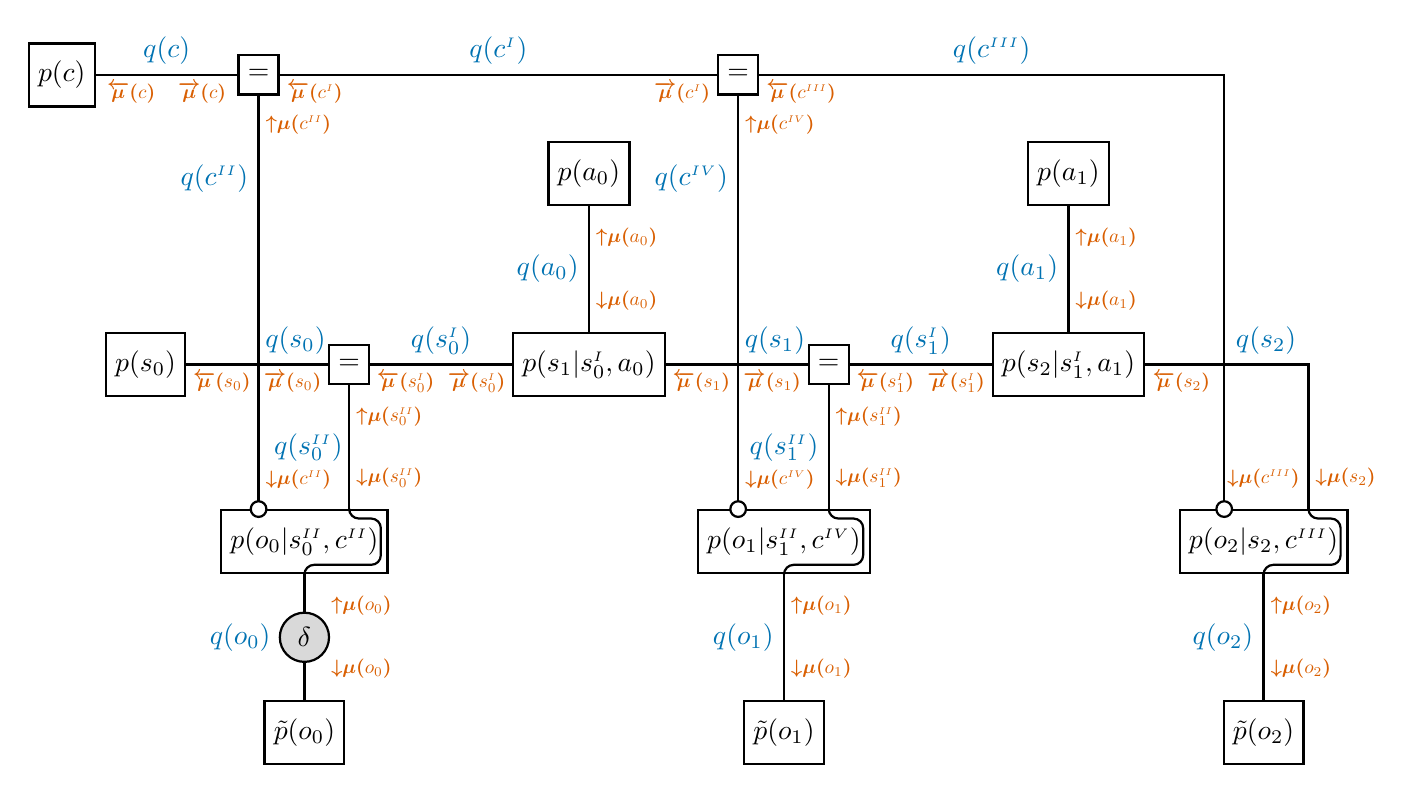
\begin{tikzpicture}[
                factor/.style={draw=black, thick, rectangle, minimum size=0.8cm, font=\normalsize},
                eqfactor/.style={draw=black, thick, rectangle, minimum size=0.5cm, font=\normalsize},
                edge/.style={thick},
                varlabel/.style={font=\normalsize},
                greycircle/.style={draw=black, thick, circle, fill=gray!30, minimum size=0.5cm, font=\normalsize}
            ]

            % Knoten
            \node[factor] (d) {$p(s_0)$};
            \node[eqfactor, right=1.8cm of d] (eq0) {$=$};
            \node[factor] (A0) at ([xshift=1.5cm, yshift=-2.25cm] d.east) {$p(o_0|s^{\scriptscriptstyle II}_0,c^{\scriptscriptstyle II})$};
            \node[factor, below=1.6cm of A0] (c0) {$\tilde{p}(o_0)$};
            \node[factor, right=1.8cm of eq0] (B0) {$p(s_1|s^{\scriptscriptstyle I}_0,a_0)$};
            \node[eqfactor, right=1.8cm of B0] (eq1) {$=$};
            \node[factor] (A1) at ([xshift=1.5cm, yshift=-2.25cm] B0.east) {$p(o_1|s^{\scriptscriptstyle II}_1,c^{\scriptscriptstyle IV})$};
            \node[factor, below=1.6cm of A1] (c1) {$\tilde{p}(o_1)$};
            \node[factor, right=1.8cm of eq1] (B1) {$p(s_2|s^{\scriptscriptstyle I}_1,a_1)$};
            \node[factor] (A2) at ([xshift=1.5cm] B1.east |- A1) {$p(o_2|s_2,c^{\scriptscriptstyle III})$};
            \node[factor, below=1.6cm of A2] (c2) {$\tilde{p}(o_2)$};
            \node[factor, above=1.6cm of B0] (u0) {$p(a_0)$};
            \node[factor, above=1.6cm of B1] (u1) {$p(a_1)$};
            \node[eqfactor, above right=3cm and 0.65cm of d] (eq3) {$=$};
            \node[eqfactor, above right=3cm and 0.65cm of B0] (eq4) {$=$};
            \node[factor, left=1.8cm of eq3] (dc) {$p(c)$};

            % Kanten zwischen Knoten
            \draw[edge] (d.east) -- (eq0.west) node[pos=0.77, above, varlabel] {$\textcolor{accblue}{q(s_0)}$} node[near start, below, varlabel, scale=0.7] {$\textcolor{accorange}{\bm{\overleftarrow{\mu}(}s_0\bm{)}}$} node[near end, below, varlabel, scale=0.7] {$\textcolor{accorange}{\bm{\overrightarrow{\mu}(}s_0\bm{)}}$};
            \draw[edge] (eq0.south) -- (eq0.south |- A0.north) node[midway, left=-0.05, varlabel] {$\textcolor{accblue}{q(s^{\scriptscriptstyle II}_0)}$} node[pos=0.25, right, varlabel, scale=0.7] {$\textcolor{accorange}{\bm{{\uparrow}{\mu}(}s^{\scriptscriptstyle II}_0\bm{)}}$} node[pos=0.75, right, varlabel, scale=0.7] {$\textcolor{accorange}{\bm{{\downarrow}{\mu}(}s^{\scriptscriptstyle II}_0\bm{)}}$};
            \draw[edge] (A0.south) -- (c0.north) node[midway, greycircle] {$\delta$} node[midway, left=0.3, varlabel] {$\textcolor{accblue}{q(o_0)}$} node[pos=0.25, right=0.25, varlabel, scale=0.7] {$\textcolor{accorange}{\bm{{\uparrow}{\mu}(}o_0\bm{)}}$} node[pos=0.75, right=0.25, varlabel, scale=0.7] {$\textcolor{accorange}{\bm{{\downarrow}{\mu}(}o_0\bm{)}}$};
            \draw[edge] (eq0.east) -- (B0.west) node[midway, above, varlabel] {$\textcolor{accblue}{q(s^{\scriptscriptstyle I}_0)}$} node[near start, below, varlabel, scale=0.7] {$\textcolor{accorange}{\bm{\overleftarrow{\mu}(}s^{\scriptscriptstyle I}_0\bm{)}}$} node[near end, below, varlabel, scale=0.7] {$\textcolor{accorange}{\bm{\overrightarrow{\mu}(}s^{\scriptscriptstyle I}_0\bm{)}}$};
            \draw[edge] (B0.north) -- (u0.south) node[midway, left, varlabel] {$\textcolor{accblue}{q(a_0)}$} node[pos=0.75, right, varlabel, scale=0.7] {$\textcolor{accorange}{\bm{{\uparrow}{\mu}(}a_0\bm{)}}$} node[pos=0.25, right, varlabel, scale=0.7] {$\textcolor{accorange}{\bm{{\downarrow}{\mu}(}a_0\bm{)}}$};
            \draw[edge] (B0.east) -- (eq1.west) node[pos=0.77, above, varlabel] {$\textcolor{accblue}{q(s_1)}$} node[near start, below, varlabel, scale=0.7] {$\textcolor{accorange}{\bm{\overleftarrow{\mu}(}s_1\bm{)}}$} node[near end, below, varlabel, scale=0.7] {$\textcolor{accorange}{\bm{\overrightarrow{\mu}(}s_1\bm{)}}$};
            \draw[edge] (eq1.south) -- (eq1.south |- A1.north) node[midway, left, varlabel] {$\textcolor{accblue}{q(s^{\scriptscriptstyle II}_1)}$} node[pos=0.25, right, varlabel, scale=0.7] {$\textcolor{accorange}{\bm{{\uparrow}{\mu}(}s^{\scriptscriptstyle II}_1\bm{)}}$} node[pos=0.75, right, varlabel, scale=0.7] {$\textcolor{accorange}{\bm{{\downarrow}{\mu}(}s^{\scriptscriptstyle II}_1\bm{)}}$};
            \draw[edge] (A1.south) -- (c1.north) node[midway, left, varlabel] {$\textcolor{accblue}{q(o_1)}$} node[pos=0.25, right, varlabel, scale=0.7] {$\textcolor{accorange}{\bm{{\uparrow}{\mu}(}o_1\bm{)}}$} node[pos=0.75, right, varlabel, scale=0.7] {$\textcolor{accorange}{\bm{{\downarrow}{\mu}(}o_1\bm{)}}$};
            \draw[edge] (eq1.east) -- (B1.west) node[midway, above, varlabel] {$\textcolor{accblue}{q(s^{\scriptscriptstyle I}_1)}$} node[near start, below, varlabel, scale=0.7] {$\textcolor{accorange}{\bm{\overleftarrow{\mu}(}s^{\scriptscriptstyle I}_1\bm{)}}$} node[near end, below, varlabel, scale=0.7] {$\textcolor{accorange}{\bm{\overrightarrow{\mu}(}s^{\scriptscriptstyle I}_1\bm{)}}$};
            \draw[edge] (B1.east) -| ([xshift=0.57cm]A2.north) node[pos=0.37, above, varlabel] {$\textcolor{accblue}{q(s_2)}$} node[pos=0.11, below, varlabel, scale=0.7] {$\textcolor{accorange}{\bm{\overleftarrow{\mu}(}s_2\bm{)}}$} node[pos=0.89, right, varlabel, scale=0.7] {$\textcolor{accorange}{\bm{{\downarrow}{\mu}(}s_2\bm{)}}$};
            \draw[edge] (A2.south) -- (c2.north) node[midway, left, varlabel] {$\textcolor{accblue}{q(o_2)}$} node[pos=0.25, right, varlabel, scale=0.7] {$\textcolor{accorange}{\bm{{\uparrow}{\mu}(}o_2\bm{)}}$} node[pos=0.75, right, varlabel, scale=0.7] {$\textcolor{accorange}{\bm{{\downarrow}{\mu}(}o_2\bm{)}}$};
            \draw[edge] (B1.north) -- (u1.south) node[midway, left, varlabel] {$\textcolor{accblue}{q(a_1)}$} node[pos=0.75, right, varlabel, scale=0.7] {$\textcolor{accorange}{\bm{{\uparrow}{\mu}(}a_1\bm{)}}$} node[pos=0.25, right, varlabel, scale=0.7] {$\textcolor{accorange}{\bm{{\downarrow}{\mu}(}a_1\bm{)}}$};
            \draw[edge] (dc.east) -- (eq3.west) node[midway, above, varlabel] {$\textcolor{accblue}{q(c)}$} node[near start, below, varlabel, scale=0.7] {$\textcolor{accorange}{\bm{\overleftarrow{\mu}(}c\bm{)}}$} node[near end, below, varlabel, scale=0.7] {$\textcolor{accorange}{\bm{\overrightarrow{\mu}(}c\bm{)}}$};
            \draw[edge] (eq3.east) -- (eq4.west) node[midway, above, varlabel] {$\textcolor{accblue}{q(c^{\scriptscriptstyle I})}$} node[pos=0.08, below, varlabel, scale=0.7] {$\textcolor{accorange}{\bm{\overleftarrow{\mu}(}c^{\scriptscriptstyle I}\bm{)}}$} node[pos=0.92, below, varlabel, scale=0.7] {$\textcolor{accorange}{\bm{\overrightarrow{\mu}(}c^{\scriptscriptstyle I}\bm{)}}$};
            \draw[edge] (eq4.east) -| ([xshift=-0.5cm]A2.north) node[pos=0.25, above, varlabel] {$\textcolor{accblue}{q(c^{\scriptscriptstyle III})}$} node[pos=0.045, below, varlabel, scale=0.7] {$\textcolor{accorange}{\bm{\overleftarrow{\mu}(}c^{\scriptscriptstyle III}\bm{)}}$} node[pos=0.965, right=-0.05, varlabel, scale=0.7] {$\textcolor{accorange}{\bm{{\downarrow}{\mu}(}c^{\scriptscriptstyle III}\bm{)}}$} node[pos=1, circle, draw=black, fill=white, inner sep=2pt] {};
            \draw[edge] (eq3.south) -- (eq3.south |- A0.north) node[pos=0.2, left, varlabel] {$\textcolor{accblue}{q(c^{\scriptscriptstyle II})}$} node[pos=0.07, right, varlabel, scale=0.7] {$\textcolor{accorange}{\bm{{\uparrow}{\mu}(}c^{\scriptscriptstyle II}\bm{)}}$} node[pos=0.93, right, varlabel, scale=0.7] {$\textcolor{accorange}{\bm{{\downarrow}{\mu}(}c^{\scriptscriptstyle II}\bm{)}}$} node[pos=1, circle, draw=black, fill=white, inner sep=2pt] {};
            \draw[edge] (eq4.south) -- (eq4.south |- A1.north) node[pos=0.2, left, varlabel] {$\textcolor{accblue}{q(c^{\scriptscriptstyle IV})}$} node[pos=0.07, right, varlabel, scale=0.7] {$\textcolor{accorange}{\bm{{\uparrow}{\mu}(}c^{\scriptscriptstyle IV}\bm{)}}$} node[pos=0.93, right, varlabel, scale=0.7] {$\textcolor{accorange}{\bm{{\downarrow}{\mu}(}c^{\scriptscriptstyle IV}\bm{)}}$} node[pos=1, circle, draw=black, fill=white, inner sep=2pt] {};

            \draw[edge, rounded corners=3.5pt]
            (eq0.south |- A0.north)
            -- ([yshift=-0.12cm]eq0.south |- A0.north)
            -| ([xshift=-0.1cm]A0.east)
            |- ([yshift=0.12cm]A0.south)
            -- (A0.south);

            \draw[edge, rounded corners=3.5pt]
            (eq1.south |- A1.north)
            -- ([yshift=-0.12cm]eq1.south |- A1.north)
            -| ([xshift=-0.1cm]A1.east)
            |- ([yshift=0.12cm]A1.south)
            -- (A1.south);

            \draw[edge, rounded corners=3.5pt]
            ([xshift=0.57cm]A2.north)
                -- ([xshift=0.57cm, yshift=-0.12cm]A2.north)
            -| ([xshift=-0.1cm]A2.east)
            |- ([yshift=0.12cm]A2.south)
            -- (A2.south);

        \end{tikzpicture}
    }
    \caption{Factor Graph of the context-BFE agent with variables' belief distributions \(\textcolor{accblue}{q}\) and messages \(\textcolor{accorange}{\mu}\).}
    \label{fig:35}
\end{figure}

Importantly, likelihood nodes send structured variational messages to break the cyclic dependencies introduced by the additional context state.  Similarly to the GFE agent these special messages of the context-BFE agent also requires recursive execution of the algorithm until convergence of the belief distributions. Moreover, the distributions \(q(o_0,s^{\scriptscriptstyle II}_0)\), \(q(o_1,s^{\scriptscriptstyle II}_1)\), \(q(o_2,s_2)\), \(q(c^{\scriptscriptstyle II})\), \(q(c^{\scriptscriptstyle IV})\), and \(q(c^{\scriptscriptstyle III})\) must be initialized (e.g., uniformly) before execution.
The resulting algorithm is given in \cref{alg:4}.
\begin{algorithm}[htbp]
    \caption{Message Passing Algorithm of the Context-BFE Agent}
    \label{alg:4}
    \small
    \begin{algorithmic}[1] % Die [1] sorgt für automatische Zeilennummern!
        \linespread{1.4}\selectfont
        \setlength{\leftskip}{0.3cm}
        \State \tikzmark{algtop4}$\textcolor{accorange}{\bm{\overrightarrow{\mu}(}s_0\bm{)}} \propto p(s_0)$,\quad$\textcolor{accorange}{\bm{{\uparrow}{\mu}(}o_0\bm{)}} \propto \delta_{o_0,\hat{o_0}}$,\quad$\textcolor{accorange}{\bm{{\downarrow}{\mu}(}a_0\bm{)}} \propto p(a_0)$,\quad$\textcolor{accorange}{\bm{{\uparrow}{\mu}(}o_1\bm{)}} \propto \tilde{p}(o_1)$,\quad$\textcolor{accorange}{\bm{{\downarrow}{\mu}(}a_1\bm{)}} \propto p(a_1)$,
        \Statex $\textcolor{accorange}{\bm{{\uparrow}{\mu}(}c^{\scriptscriptstyle II}\bm{)}} \propto \exp \left( \sum_{o_0,s^{\scriptscriptstyle II}_0} q(o_0,s^{\scriptscriptstyle II}_0) \ln p(o_0|s^{\scriptscriptstyle II}_0,c^{\scriptscriptstyle II}) \right)$,\quad$\textcolor{accorange}{\bm{{\downarrow}{\mu}(}o_0\bm{)}} \propto \delta_{o_0,\hat{o_0}}$,
        \Statex $\textcolor{accorange}{\bm{{\uparrow}{\mu}(}c^{\scriptscriptstyle IV}\bm{)}} \propto \exp \left( \sum_{o_1,s^{\scriptscriptstyle II}_1} q(o_1,s^{\scriptscriptstyle II}_1) \ln p(o_1|s^{\scriptscriptstyle II}_1,c^{\scriptscriptstyle IV}) \right)$,\quad$\textcolor{accorange}{\bm{{\uparrow}{\mu}(}o_2\bm{)}} \propto \tilde{p}(o_2)$,
        \Statex $\textcolor{accorange}{\bm{\overleftarrow{\mu}(}c^{\scriptscriptstyle III}\bm{)}} \propto \exp \left( \sum_{o_2,s_2} q(o_2,s_2) \ln p(o_2|s_2,c^{\scriptscriptstyle III}) \right)$,\quad$\textcolor{accorange}{\bm{\overrightarrow{\mu}(}c\bm{)}} \propto p(c)$
        \State $\textcolor{accorange}{\bm{{\uparrow}{\mu}(}s^{\scriptscriptstyle II}_0\bm{)}} \propto \sum_{o_0} \exp \left( \sum_{c^{\scriptscriptstyle II}} q(c^{\scriptscriptstyle II}) \ln p(o_0|s^{\scriptscriptstyle II}_0,c^{\scriptscriptstyle II}) \right) \textcolor{black}{\bm{{\uparrow}{\mu}(}o_0\bm{)}}$,\quad$\textcolor{accorange}{\bm{\overrightarrow{\mu}(}c^{\scriptscriptstyle I}\bm{)}} \propto \textcolor{black}{\bm{\overrightarrow{\mu}(}c\bm{)}} \textcolor{black}{\bm{{\uparrow}{\mu}(}c^{\scriptscriptstyle II}\bm{)}}$,
        \Statex $\textcolor{accorange}{\bm{{\uparrow}{\mu}(}s^{\scriptscriptstyle II}_1\bm{)}} \propto \sum_{o_1} \exp \left( \sum_{c^{\scriptscriptstyle IV}} q(c^{\scriptscriptstyle IV}) \ln p(o_1|s^{\scriptscriptstyle II}_1,c^{\scriptscriptstyle IV}) \right) \textcolor{black}{\bm{{\uparrow}{\mu}(}o_1\bm{)}}$,\quad$\textcolor{accorange}{\bm{\overleftarrow{\mu}(}c^{\scriptscriptstyle I}\bm{)}} \propto \textcolor{black}{\bm{{\uparrow}{\mu}(}c^{\scriptscriptstyle IV}\bm{)}} \textcolor{black}{\bm{\overleftarrow{\mu}(}c^{\scriptscriptstyle III}\bm{)}}$,
        \Statex $\textcolor{accorange}{\bm{\overleftarrow{\mu}(}s_2\bm{)}} \propto \sum_{o_2} \exp \left( \sum_{c^{\scriptscriptstyle III}} q(c^{\scriptscriptstyle III}) \ln p(o_2|s_2,c^{\scriptscriptstyle III}) \right) \textcolor{black}{\bm{{\uparrow}{\mu}(}o_2\bm{)}}$
        \State $\textcolor{accorange}{\bm{\overrightarrow{\mu}(}s^{\scriptscriptstyle I}_0\bm{)}} \propto \sum_{s_0,s^{\scriptscriptstyle II}_0} \delta_{s_0,s^{\scriptscriptstyle I}_0}\delta_{s_0,s^{\scriptscriptstyle II}_0} \textcolor{black}{\bm{\overrightarrow{\mu}(}s_0\bm{)}} \textcolor{black}{\bm{{\uparrow}{\mu}(}s^{\scriptscriptstyle II}_0\bm{)}}$,\quad$\textcolor{accorange}{\bm{{\downarrow}{\mu}(}c^{\scriptscriptstyle III}\bm{)}} \propto \textcolor{black}{\bm{\overrightarrow{\mu}(}c^{\scriptscriptstyle I}\bm{)}} \textcolor{black}{\bm{{\uparrow}{\mu}(}c^{\scriptscriptstyle IV}\bm{)}}$,
        \Statex $\textcolor{accorange}{\bm{\overleftarrow{\mu}(}s^{\scriptscriptstyle I}_1\bm{)}} \propto \sum_{a_1,s_2} p(s_2|s^{\scriptscriptstyle I}_1,a_1) \textcolor{black}{\bm{{\downarrow}{\mu}(}a_1\bm{)}} \textcolor{black}{\bm{\overleftarrow{\mu}(}s_2\bm{)}}$,\quad$\textcolor{accorange}{\bm{{\downarrow}{\mu}(}c^{\scriptscriptstyle IV}\bm{)}} \propto \textcolor{black}{\bm{\overrightarrow{\mu}(}c^{\scriptscriptstyle I}\bm{)}} \textcolor{black}{\bm{\overleftarrow{\mu}(}c^{\scriptscriptstyle III}\bm{)}}$,
        \Statex $\textcolor{accorange}{\bm{{\downarrow}{\mu}(}c^{\scriptscriptstyle II}\bm{)}} \propto \textcolor{black}{\bm{\overrightarrow{\mu}(}c\bm{)}} \textcolor{black}{\bm{\overleftarrow{\mu}(}c^{\scriptscriptstyle I}\bm{)}}$,\quad$\textcolor{accorange}{\bm{\overleftarrow{\mu}(}c\bm{)}} \propto \textcolor{black}{\bm{{\uparrow}{\mu}(}c^{\scriptscriptstyle II}\bm{)}} \textcolor{black}{\bm{\overleftarrow{\mu}(}c^{\scriptscriptstyle I}\bm{)}}$
        \State $\textcolor{accorange}{\bm{\overrightarrow{\mu}(}s_1\bm{)}} \propto \sum_{s^{\scriptscriptstyle I}_0,a_0} p(s_1|s^{\scriptscriptstyle I}_0,a_0) \textcolor{black}{\bm{\overrightarrow{\mu}(}s^{\scriptscriptstyle I}_0\bm{)}} \textcolor{black}{\bm{{\downarrow}{\mu}(}a_0\bm{)}}$,\quad$\textcolor{accorange}{\bm{\overleftarrow{\mu}(}s_1\bm{)}} \propto \sum_{s^{\scriptscriptstyle I}_1,s^{\scriptscriptstyle II}_1} \delta_{s_1,s^{\scriptscriptstyle I}_1}\delta_{s_1,s^{\scriptscriptstyle II}_1} \textcolor{black}{\bm{\overleftarrow{\mu}(}s^{\scriptscriptstyle I}_1\bm{)}} \textcolor{black}{\bm{{\uparrow}{\mu}(}s^{\scriptscriptstyle II}_1\bm{)}}$
        \State $\textcolor{accorange}{\bm{\overrightarrow{\mu}(}s^{\scriptscriptstyle I}_1\bm{)}} \propto \sum_{s_1,s^{\scriptscriptstyle II}_1} \delta_{s_1,s^{\scriptscriptstyle I}_1}\delta_{s_1,s^{\scriptscriptstyle II}_1} \textcolor{black}{\bm{\overrightarrow{\mu}(}s_1\bm{)}} \textcolor{black}{\bm{{\uparrow}{\mu}(}s^{\scriptscriptstyle II}_1\bm{)}}$,\quad$\textcolor{accorange}{\bm{{\downarrow}{\mu}(}s^{\scriptscriptstyle II}_1\bm{)}} \propto \sum_{s_1,s^{\scriptscriptstyle I}_1} \delta_{s_1,s^{\scriptscriptstyle I}_1}\delta_{s_1,s^{\scriptscriptstyle II}_1} \textcolor{black}{\bm{\overrightarrow{\mu}(}s_1\bm{)}} \textcolor{black}{\bm{\overleftarrow{\mu}(}s^{\scriptscriptstyle I}_1\bm{)}}$,
        \Statex $\textcolor{accorange}{\bm{{\uparrow}{\mu}(}a_0\bm{)}} \propto \sum_{s_1,s^{\scriptscriptstyle I}_0} p(s_1|s^{\scriptscriptstyle I}_0,a_0) \textcolor{black}{\bm{\overrightarrow{\mu}(}s^{\scriptscriptstyle I}_0\bm{)}} \textcolor{black}{\bm{\overleftarrow{\mu}(}s_1\bm{)}}$,\quad$\textcolor{accorange}{\bm{\overleftarrow{\mu}(}s^{\scriptscriptstyle I}_0\bm{)}} \propto \sum_{s_1,a_0} p(s_1|s^{\scriptscriptstyle I}_0,a_0) \textcolor{black}{\bm{{\downarrow}{\mu}(}a_0\bm{)}} \textcolor{black}{\bm{\overleftarrow{\mu}(}s_1\bm{)}}$
        \State $\textcolor{accorange}{\bm{{\uparrow}{\mu}(}a_1\bm{)}} \propto \sum_{s^{\scriptscriptstyle I}_1,s_2} p(s_2|s^{\scriptscriptstyle I}_1,a_1) \textcolor{black}{\bm{\overrightarrow{\mu}(}s^{\scriptscriptstyle I}_1\bm{)}} \textcolor{black}{\bm{\overleftarrow{\mu}(}s_2\bm{)}}$,\quad$\textcolor{accorange}{\bm{{\downarrow}{\mu}(}s_2\bm{)}} \propto \sum_{s^{\scriptscriptstyle I}_1,a_1} p(s_2|s^{\scriptscriptstyle I}_1,a_1) \textcolor{black}{\bm{\overrightarrow{\mu}(}s^{\scriptscriptstyle I}_1\bm{)}} \textcolor{black}{\bm{{\downarrow}{\mu}(}a_1\bm{)}}$,
        \Statex $\textcolor{accorange}{\bm{{\downarrow}{\mu}(}o_1\bm{)}} \propto \sum_{s^{\scriptscriptstyle II}_1} \exp \left( \sum_{c^{\scriptscriptstyle IV}} q(c^{\scriptscriptstyle IV}) \ln p(o_1|s^{\scriptscriptstyle II}_1,c^{\scriptscriptstyle IV}) \right) \textcolor{black}{\bm{{\downarrow}{\mu}(}s^{\scriptscriptstyle II}_1\bm{)}}$,
        \Statex $\textcolor{accorange}{\bm{\overleftarrow{\mu}(}s_0\bm{)}} \propto \sum_{s^{\scriptscriptstyle I}_0,s^{\scriptscriptstyle II}_0} \delta_{s_0,s^{\scriptscriptstyle I}_0}\delta_{s_0,s^{\scriptscriptstyle II}_0} \textcolor{black}{\bm{\overleftarrow{\mu}(}s^{\scriptscriptstyle I}_0\bm{)}} \textcolor{black}{\bm{{\uparrow}{\mu}(}s^{\scriptscriptstyle II}_0\bm{)}}$,\quad$\textcolor{accorange}{\bm{{\downarrow}{\mu}(}s^{\scriptscriptstyle II}_0\bm{)}} \propto \sum_{s_0,s^{\scriptscriptstyle I}_0} \delta_{s_0,s^{\scriptscriptstyle I}_0}\delta_{s_0,s^{\scriptscriptstyle II}_0} \textcolor{black}{\bm{\overrightarrow{\mu}(}s_0\bm{)}} \textcolor{black}{\bm{\overleftarrow{\mu}(}s^{\scriptscriptstyle I}_0\bm{)}}$
        \State $\textcolor{accorange}{\bm{{\downarrow}{\mu}(}o_2\bm{)}} \propto \sum_{s_2} \exp \left( \sum_{c^{\scriptscriptstyle III}} q(c^{\scriptscriptstyle III}) \ln p(o_2|s_2,c^{\scriptscriptstyle III}) \right) \textcolor{black}{\bm{{\downarrow}{\mu}(}s_2\bm{)}}$
        \State \tikzmark{algbottom4}$\textcolor{accblue}{q(s_0)} \propto \textcolor{black}{\bm{\overleftarrow{\mu}(}s_0\bm{)}} \textcolor{black}{\bm{\overrightarrow{\mu}(}s_0\bm{)}}$,\quad$\textcolor{accblue}{q(s^{\scriptscriptstyle I}_0)} \propto \textcolor{black}{\bm{\overleftarrow{\mu}(}s^{\scriptscriptstyle I}_0\bm{)}} \textcolor{black}{\bm{\overrightarrow{\mu}(}s^{\scriptscriptstyle I}_0\bm{)}}$,\quad$\textcolor{accblue}{q(s^{\scriptscriptstyle II}_0)} \propto \textcolor{black}{\bm{{\uparrow}{\mu}(}s^{\scriptscriptstyle II}_0\bm{)}} \textcolor{black}{\bm{{\downarrow}{\mu}(}s^{\scriptscriptstyle II}_0\bm{)}}$,
        \Statex $\textcolor{accblue}{q(s_1)} \propto \textcolor{black}{\bm{\overleftarrow{\mu}(}s_1\bm{)}} \textcolor{black}{\bm{\overrightarrow{\mu}(}s_1\bm{)}}$,\quad$\textcolor{accblue}{q(s^{\scriptscriptstyle I}_1)} \propto \textcolor{black}{\bm{\overleftarrow{\mu}(}s^{\scriptscriptstyle I}_1\bm{)}} \textcolor{black}{\bm{\overrightarrow{\mu}(}s^{\scriptscriptstyle I}_1\bm{)}}$,\quad$\textcolor{accblue}{q(s^{\scriptscriptstyle II}_1)} \propto \textcolor{black}{\bm{{\uparrow}{\mu}(}s^{\scriptscriptstyle II}_1\bm{)}} \textcolor{black}{\bm{{\downarrow}{\mu}(}s^{\scriptscriptstyle II}_1\bm{)}}$,
        \Statex $\textcolor{accblue}{q(s_2)} \propto \textcolor{black}{\bm{\overleftarrow{\mu}(}s_2\bm{)}} \textcolor{black}{\bm{{\downarrow}{\mu}(}s_2\bm{)}}$,\quad$\textcolor{accblue}{q(a_0)} \propto \textcolor{black}{\bm{{\uparrow}{\mu}(}a_0\bm{)}} \textcolor{black}{\bm{{\downarrow}{\mu}(}a_0\bm{)}}$,\quad$\textcolor{accblue}{q(a_1)} \propto \textcolor{black}{\bm{{\uparrow}{\mu}(}a_1\bm{)}} \textcolor{black}{\bm{{\downarrow}{\mu}(}a_1\bm{)}}$,
        \Statex $\textcolor{accblue}{q(o_0)} \propto \textcolor{black}{\bm{{\uparrow}{\mu}(}o_0\bm{)}} \textcolor{black}{\bm{{\downarrow}{\mu}(}o_0\bm{)}}$,\quad$\textcolor{accblue}{q(o_1)} \propto \textcolor{black}{\bm{{\uparrow}{\mu}(}o_1\bm{)}} \textcolor{black}{\bm{{\downarrow}{\mu}(}o_1\bm{)}}$,\quad$\textcolor{accblue}{q(o_2)} \propto \textcolor{black}{\bm{{\uparrow}{\mu}(}o_2\bm{)}} \textcolor{black}{\bm{{\downarrow}{\mu}(}o_2\bm{)}}$,
        \Statex $\textcolor{accblue}{q(c)} \propto \textcolor{black}{\bm{\overleftarrow{\mu}(}c\bm{)}} \textcolor{black}{\bm{\overrightarrow{\mu}(}c\bm{)}}$,\quad$\textcolor{accblue}{q(c^{\scriptscriptstyle I})} \propto \textcolor{black}{\bm{\overleftarrow{\mu}(}c^{\scriptscriptstyle I}\bm{)}} \textcolor{black}{\bm{\overrightarrow{\mu}(}c^{\scriptscriptstyle I}\bm{)}}$,\quad$\textcolor{accblue}{q(c^{\scriptscriptstyle II})} \propto \textcolor{black}{\bm{{\uparrow}{\mu}(}c^{\scriptscriptstyle II}\bm{)}} \textcolor{black}{\bm{{\downarrow}{\mu}(}c^{\scriptscriptstyle II}\bm{)}}$,
        \Statex $\textcolor{accblue}{q(c^{\scriptscriptstyle III})} \propto \textcolor{black}{\bm{\overleftarrow{\mu}(}c^{\scriptscriptstyle III}\bm{)}} \textcolor{black}{\bm{\overrightarrow{\mu}(}c^{\scriptscriptstyle III}\bm{)}}$,\quad$\textcolor{accblue}{q(c^{\scriptscriptstyle IV})} \propto \textcolor{black}{\bm{{\uparrow}{\mu}(}c^{\scriptscriptstyle IV}\bm{)}} \textcolor{black}{\bm{{\downarrow}{\mu}(}c^{\scriptscriptstyle IV}\bm{)}}$,
        \Statex $\textcolor{black}{q(o_0,s^{\scriptscriptstyle II}_0)} \propto \exp \left( \sum_{o_0,s^{\scriptscriptstyle II}_0} q(o_0,s^{\scriptscriptstyle II}_0) \ln p(o_0|s^{\scriptscriptstyle II}_0,c^{\scriptscriptstyle II}) \right) \textcolor{black}{\bm{{\downarrow}{\mu}(}s^{\scriptscriptstyle II}_0\bm{)}} \textcolor{black}{\bm{{\uparrow}{\mu}(}o_0\bm{)}}$,
        \Statex $\textcolor{black}{q(o_1,s^{\scriptscriptstyle II}_1)} \propto \exp \left( \sum_{o_1,s^{\scriptscriptstyle II}_1} q(o_1,s^{\scriptscriptstyle II}_1) \ln p(o_1|s^{\scriptscriptstyle II}_1,c^{\scriptscriptstyle IV}) \right) \textcolor{black}{\bm{{\downarrow}{\mu}(}s^{\scriptscriptstyle II}_1\bm{)}} \textcolor{black}{\bm{{\uparrow}{\mu}(}o_1\bm{)}}$,
        \Statex $\textcolor{black}{q(o_2,s_2)} \propto \exp \left( \sum_{o_2,s_2} q(o_2,s_2) \ln p(o_2|s_2,c^{\scriptscriptstyle III}) \right) \textcolor{black}{\bm{{\downarrow}{\mu}(}s_2\bm{)}} \textcolor{black}{\bm{{\uparrow}{\mu}(}o_2\bm{)}}$
    \end{algorithmic}

    \begin{tikzpicture}[remember picture, overlay]
        \draw[-{Stealth[length=2.2mm, width=1.6mm]}, thick, gray!75!black, rounded corners=5pt]
        ([yshift=0.5ex, xshift=-2.5ex]pic cs:algbottom4) -- ++(-0.4cm, 0) |- ([xshift=-2.5ex, yshift=0.5ex]pic cs:algtop4);
    \end{tikzpicture}

\end{algorithm}


\subsection{Context-GFE Agent}

In this section I present the derivation of GFE-based messages for the context state \(c\). Following this, the resulting Context-GFE agent will be able to reduce its uncertainty regarding the context state rather than only the hidden state \(s\), which is the central goal of this thesis. The agent is based on the same generative model as the Context-BFE agent, i.e., \cref{eq:35}, and consequently also utilizes the same foundational factor graph (\cref{fig:28}). Interestingly, the derivation also leads to GFE-based messages for the hidden state \(s\), although this was not the central goal. It can be suspected that this circumstance is based on the independence assumption between hidden state \(s\) and the other two variables \(c\) and \(o\) that is made during the derivation.

\subsubsection{GFE-Based Messages for the Context}

In this section I derive the GFE-based message (\(\textcolor{accorange}{\bm{{\uparrow}{\mu}(}c\bm{)}}\) in \cref{fig:36.2}) that is sent by future likelihood nodes upwards to transition nodes and enables the agent with contextual information seeking (also including the GFE-based message \(\textcolor{black}{\bm{{\uparrow}{\mu}(}s\bm{)}}\)).

\begin{figure}[htbp]
    \centering
    \begin{subfigure}[t]{0.48\textwidth}
        \centering
        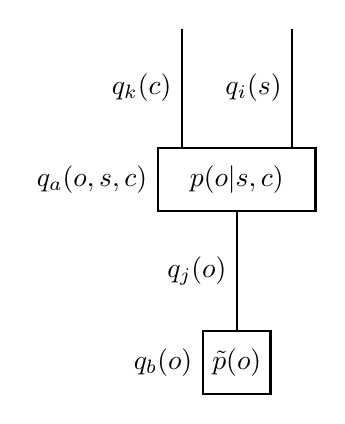
\begin{tikzpicture}[
                factor/.style={draw=black, thick, rectangle, minimum size=0.8cm, font=\normalsize},
                eqfactor/.style={draw=black, thick, rectangle, minimum size=0.5cm, font=\normalsize},
                edge/.style={thick},
                varlabel/.style={font=\normalsize},
                greycircle/.style={draw=black, thick, circle, fill=gray!30, minimum size=0.5cm, font=\normalsize}
            ]

            % Knoten
            \node[factor, minimum width=2.0cm, label={[varlabel]left:$q_a(o,s,c)$}] (A1) {$p(o|s,c)$};
            \node[factor, below=1.5cm of A1, label={[varlabel]left:$q_b(o)$}] (c1) {$\tilde{p}(o)$};

            % Kanten zwischen Knoten
            \draw[edge] ([yshift=1.5cm,xshift=0.7cm]A1.north) -- ([xshift=0.7cm]A1.north) node[midway, left, varlabel] {$q_i(s)$};
            \draw[edge] (A1.south) -- (c1.north) node[midway, left, varlabel] {$q_j(o)$};
            \draw[edge] ([yshift=1.5cm,xshift=-0.7cm]A1.north) -- ([xshift=-0.7cm]A1.north) node[midway, left, varlabel] {$q_k(c)$};

        \end{tikzpicture}
        \caption{Perception-related factor graph sector with Bethe free energy.}
        \label{fig:36.1}
    \end{subfigure}
    \hfill
    \begin{subfigure}[t]{0.48\textwidth}
        \centering
        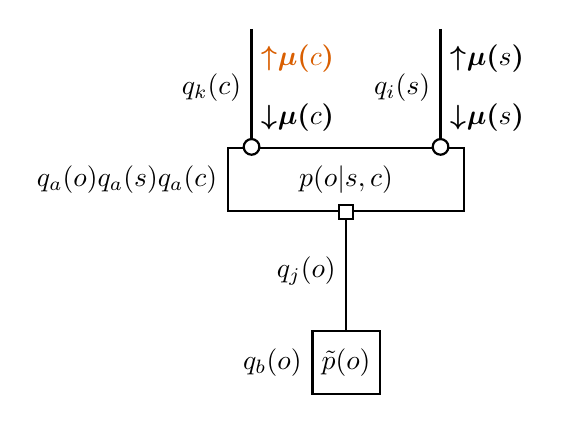
\begin{tikzpicture}[
                factor/.style={draw=black, thick, rectangle, minimum size=0.8cm, font=\normalsize},
                eqfactor/.style={draw=black, thick, rectangle, minimum size=0.5cm, font=\normalsize},
                edge/.style={thick},
                varlabel/.style={font=\normalsize},
                greycircle/.style={draw=black, thick, circle, fill=gray!30, minimum size=0.5cm, font=\normalsize}
            ]

            % Knoten
            \node[factor, minimum width=3.0cm, label={[varlabel]left:$q_a(o)q_a(s)q_a(c)$}] (A1) {$p(o|s,c)$};
            \node[factor, below=1.5cm of A1, label={[varlabel]left:$q_b(o)$}] (c1) {$\tilde{p}(o)$};

            % Kanten zwischen Knoten
            \draw[edge] ([yshift=1.5cm,xshift=1.2cm]A1.north) -- ([xshift=1.2cm]A1.north) node[midway, left, varlabel] {$q_i(s)$} node[pos=0.25, right, varlabel] {$\textcolor{black}{\bm{{\uparrow}{\mu}(}s\bm{)}}$} node[pos=0.75, right, varlabel] {$\bm{{\downarrow}{\mu}(}s\bm{)}$} {} node[pos=1, circle, draw=black, fill=white, inner sep=2pt] {};
            \draw[edge] (A1.south) -- (c1.north) node[midway, left, varlabel] {$q_j(o)$} node[pos=0, rectangle, draw=black, fill=white, inner sep=2.5pt] {};
            \draw[edge] ([yshift=1.5cm,xshift=-1.2cm]A1.north) -- ([xshift=-1.2cm]A1.north) node[midway, left, varlabel] {$q_k(c)$} node[pos=0.25, right, varlabel] {$\textcolor{accorange}{\bm{{\uparrow}{\mu}(}c\bm{)}}$} node[pos=0.75, right, varlabel] {$\bm{{\downarrow}{\mu}(}c\bm{)}$} node[pos=1, circle, draw=black, fill=white, inner sep=2pt] {};

        \end{tikzpicture}
        \caption{Perception-related factor graph sector with generalized free energy and corresponding GFE-based message (\(\textcolor{accorange}{\bm{{\uparrow}{\mu}(}c\bm{)}}\)) for  contextual information seeking.}
        \label{fig:36.2}
    \end{subfigure}
    \caption{Perception-related factor graph sectors.}
    \label{fig:36}
\end{figure}

Starting point for this derivation is the Lagrangian \(L\) of this perception-related factor graph sector with Bethe free energy (\cref{fig:36.1}):
\begin{alignat}{2}
    L = & \sum_{o,s,c} q_a(o,s,c) \ln \frac{q_a(o,s,c)}{p(o|s,c)} + \sum_o q_b(o) \ln \frac{q_b(o)}{\tilde{p}(o)} + \sum_o q_j(o) \ln \frac{1}{q_j(o)} \nonumber \\
        & + \sum_c \lambda_{ka}(c) \left( q_k(c) - \sum_{o,s} q_a(o,s,c) \right) + \sum_s \lambda_{ia}(s) \left( q_i(s) - \sum_{o,c} q_a(o,s,c) \right) \nonumber \\
        & + \sum_o \lambda_{ja}(o) \left( q_j(o) - \sum_{s,c} q_a(o,s,c) \right) + \sum_o \lambda_{jb}(o) \left( q_j(o) - \sum_{s,c} q_a(o,s,c) \right)
\end{alignat}

Similar to the GFE-based messages (\cref{sec:gfe}) we also introduce a mutual information term to the Lagrangian. In this case the term accounts for the variables \(o\) and \(c\), which means the agent is inclined to reduce its contextual uncertainty from observations. The resulting Lagrangain \(L_{\text{MI}}\) is:
\begin{equation}
    L_{\text{MI}} = L + \sum_{o,s} q_a(o,s) \ln \frac{q_a(o)q_a(s)}{q_a(o,s)}
\end{equation}

Next, we add \(0 = \sum_s q_a(s) \ln \frac{q_a(s)}{q_a(s)}\) to \(L_{\text{MI}}\) and also assume independence between \(s\) and the two variables \(o\) and \(c\), i.e., \(q_a(o,s,c) = q_a(o,c)q_a(s)\), which allows for the following rearrangement of \(L_{\text{MI}}\) (compare with \cref{sec:gfe}):
\begin{alignat}{2}
    L_{\text{MI}} = & \sum_{o,s,c} q_a(o,s,c) \ln \frac{q_a(o)q_a(c)q_a(s)}{p(o|s,c)\tilde{p}(o)} \nonumber \\
    & + \sum_c \lambda_{ka}(c) \left( q_k(c) - \sum_{o,s} q_a(o,s,c) \right) + \sum_s \lambda_{ia}(s) \left( q_i(s) - \sum_{o,c} q_a(o,s,c) \right)
\end{alignat}

Next, we perform the p-substitution from \cref{sec:gfe}. Together with \(q_a(o,s,c) = q_a(o,c)q_a(s) \Rightarrow q_a(s,c) = q_a(s)q_a(c)\) it follows (\(L_{\text{GFE}}\)):
\begin{alignat}{2}
    L_{\text{GFE}} = & \sum_{o,s,c} p(o|s,c)q_a(s)q_a(c) \ln \frac{q_a(o)q_a(c)q_a(s)}{p(o|s,c)\tilde{p}(o)} \nonumber \\
    & + \sum_c \lambda_{ka}(c) \left( q_k(c) - \sum_{o,s} q_a(o,s,c) \right) + \sum_s \lambda_{ia}(s) \left( q_i(s) - \sum_{o,c} q_a(o,s,c) \right)
\end{alignat}

Next, the Lagrangian is differentiated with respect to \(q_a(c)\), set to \(0\), and finally solved for \(q^*_a(c)\):
\begin{alignat}{3}
     & \frac{\delta L_{\text{GFE}}}{\delta q_a(c)} &  & = \sum_{o,s} p(o|s,c)q_a(s) \ln \frac{q_a(o)}{p(o|s,c)\tilde{p}(o)} + \ln q_a(c) + 1 - \lambda_{ka}(c) \overset{!}{=} 0                                \\
     &                                             &  & \Rightarrow q^*_a(c) \propto \exp \left( \sum_{o,s} p(o|s,c)q_a(s) \ln \frac{p(o|s,c)\tilde{p}(o)}{q_a(o)} \right) \exp \left( \lambda_{ka}(c) \right)
\end{alignat}

Finally, we use the result of \cref{sec:1} for the local stationary point of \(q_k(c)\)
\begin{equation}
    q^*_k(c) \propto \exp \left( \lambda_{ka}(c) \right) \exp \left( \lambda_{k\bullet}(c) \right),
\end{equation}
and use the marginalization constraint \(q_k(c) \overset{!}{=} q_a(c)\) to determine the message \(\textcolor{accorange}{\bm{{\uparrow}{\mu}(}c\bm{)}}\) that enables contextual information seeking:
\begin{alignat}{2}
    & q^*_k(c)                                                                      &  & \overset{!}{=} q^*_a(c)                                                                                               \\
    & \exp \left( \lambda_{ka}(c) \right) \exp \left( \lambda_{k\bullet}(s) \right) &  & \propto \exp \left( \sum_{o,s} p(o|s,c)q_a(s) \ln \frac{p(o|s,c)\tilde{p}(o)}{q_a(o)} \right) \exp \left( \lambda_{ka}(c) \right) \\
    & \exp \left( \lambda_{k\bullet}(c) \right)                                     &  & \propto \exp \left( \sum_{o,s} p(o|s,c)q_a(s) \ln \frac{p(o|s,c)\tilde{p}(o)}{q_a(o)} \right)                                     \\
    & \textcolor{accorange}{\bm{{\uparrow}{\mu}(}c\bm{)}}                                                  &  & \propto \exp \left( \sum_{o,s} p(o|s,c)q_a(s) \ln \frac{p(o|s,c)\tilde{p}(o)}{q_a(o)} \right)
\end{alignat}

As mentioned in \cref{sec:gfe}, using this message can lead to unstable message passing algorithms. Consequently, we also use an alternative approach that locally optimizes (via iteration index \(l\)) the message instead (details in \cref{sec:gfe}):
\begin{alignat}{2}
    &q^{(l)}_j(o) &&\propto \sum_{s,c} p(o|s,c) q_i(s) q^{(l-1)}_k(c). \label{eq:46} \\
    & \textcolor{accorange}{\bm{{\uparrow}{\mu}}^{(l)}\bm{(}c\bm{)}}                                                  &  & \propto \exp \left( \sum_{o,s} p(o|s,c)q_a(s) \ln \frac{p(o|s,c)\tilde{p}(o)}{q^{(l)}_a(o)} \right) \label{eq:47}\\
    &q^{(l)}_k(c) &&\propto \textcolor{accorange}{\bm{{\uparrow}{\mu}}^{(l)}\bm{(}c\bm{)}} \bm{{\downarrow}{\mu}(}c\bm{)} \label{eq:48}\\
    &\textcolor{accorange}{\bm{{\uparrow}{\mu}(}c\bm{)}} &&\propto \frac{q^*_k(c)}{\bm{{\downarrow}{\mu}(}c\bm{)}} \label{eq:49}
\end{alignat}
Equations \cref{eq:46,eq:47,eq:48} are iterated until convergence of \(q_k(c)\) (with \(q_j(o) = q_a(o)\)), which is then used in \cref{eq:49}.

Moreover, the Lagrangian \(L_{\text{GFE}}\) also leads to a GFE-based message \(\bm{{\uparrow}{\mu}(}s\bm{)}\), i.e., for the hidden state \(s\). The derivation is analog to the prior derivation for the GFE-based message over the context. The resulting optimization loop (analog to \cref{eq:46,eq:47,eq:48})) that leads to the message \(\bm{{\uparrow}{\mu}(}s\bm{)}\) is given in the following:
\begin{alignat}{2}
    &q^{(l)}_j(o) &&\propto \sum_{s,c} p(o|s,c) q^{(l-1)}_i(s) q_k(c). \\
    & \bm{{\uparrow}{\mu}}^{(l)}\bm{(}s\bm{)}                                                  &  & \propto \exp \left( \sum_{o,c} p(o|s,c)q_a(c) \ln \frac{p(o|s,c)\tilde{p}(o)}{q^{(l)}_a(o)} \right) \\
    &q^{(l)}_i(s) &&\propto \bm{{\uparrow}{\mu}}^{(l)}\bm{(}s\bm{)} \bm{{\downarrow}{\mu}(}s\bm{)}\\
    &\bm{{\uparrow}{\mu}(}s\bm{)} &&\propto \frac{q^*_i(s)}{\bm{{\downarrow}{\mu}(}s\bm{)}}
\end{alignat}


\subsubsection{Message Passing Algorithm}
In this section I give the message passing algorithm of the Context-GFE agent, which is based on its factor graph (\cref{fig:38}) that again exemplary includes an observation \(\hat {o_0}\). Analog to the algorithm of the GFE agent, the message passing algorithm of the Context-GFE agent also requires recursive execution and the initialization of the belief distributions \(q(o_0)\), \(q(s^{\scriptscriptstyle II}_0)\), \(q(s^{\scriptscriptstyle II}_1)\), \(q(c^{\scriptscriptstyle IV})\), \(q(s_2)\), \(q(c^{\scriptscriptstyle III})\), \(q(c^{\scriptscriptstyle II})\) and messages \(\bm{{\downarrow}{\mu}(}c^{\scriptscriptstyle IV}\bm{)}\), \(\bm{{\downarrow}{\mu}(}c^{\scriptscriptstyle III}\bm{)}\), \(\bm{{\downarrow}{\mu}(}s^{\scriptscriptstyle II}_1\bm{)}\), \(\bm{{\downarrow}{\mu}(}s_2\bm{)}\) (e.g., uniformly) before it is started. The resulting message passing algorithm of the Context-GFE agent is given in \cref{alg:5}.
\begin{figure}[htbp]
    \centering

    \resizebox{1.0\textwidth}{!}{%
        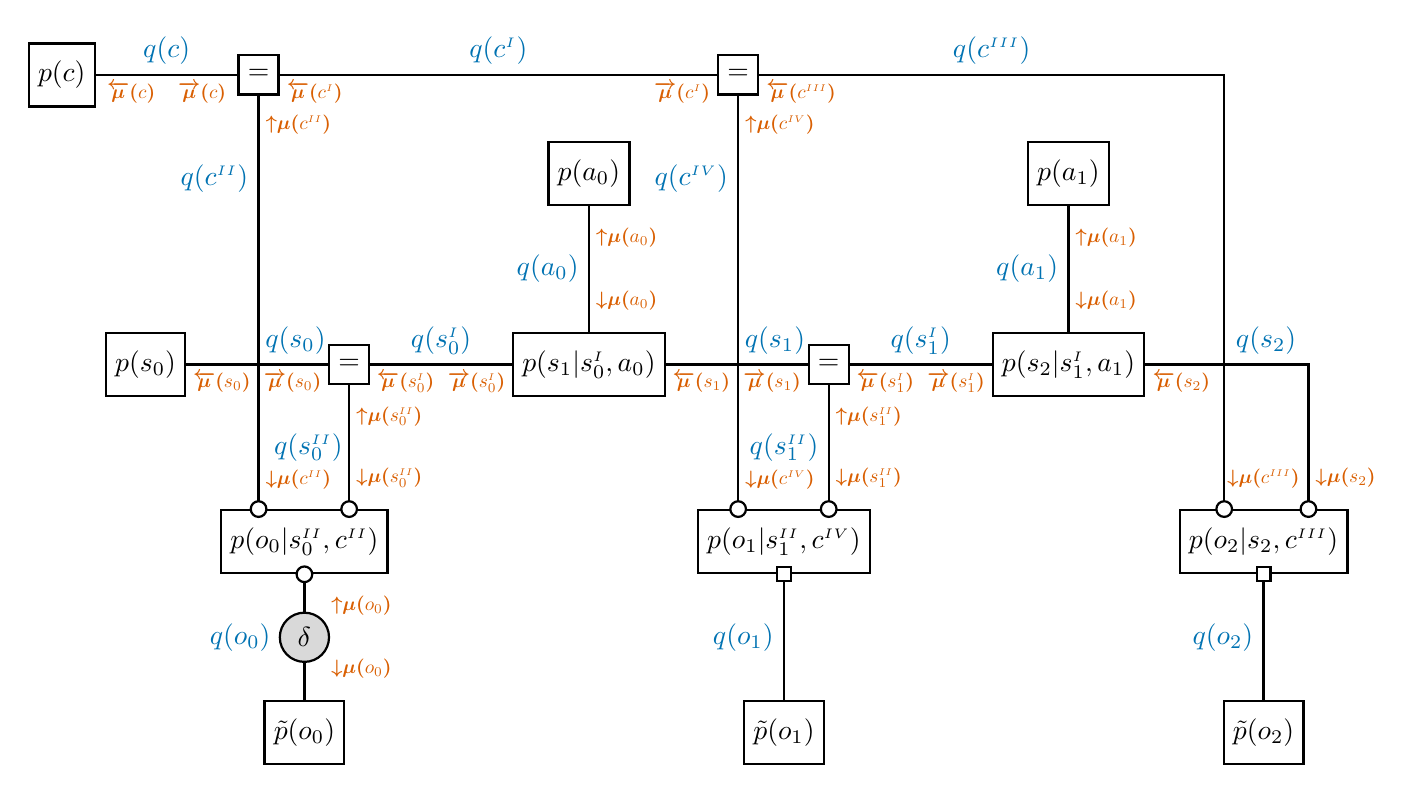
\begin{tikzpicture}[
                factor/.style={draw=black, thick, rectangle, minimum size=0.8cm, font=\normalsize},
                eqfactor/.style={draw=black, thick, rectangle, minimum size=0.5cm, font=\normalsize},
                edge/.style={thick},
                varlabel/.style={font=\normalsize},
                greycircle/.style={draw=black, thick, circle, fill=gray!30, minimum size=0.5cm, font=\normalsize}
            ]

            % Knoten
            \node[factor] (d) {$p(s_0)$};
            \node[eqfactor, right=1.8cm of d] (eq0) {$=$};
            \node[factor] (A0) at ([xshift=1.5cm, yshift=-2.25cm] d.east) {$p(o_0|s^{\scriptscriptstyle II}_0,c^{\scriptscriptstyle II})$};
            \node[factor, below=1.6cm of A0] (c0) {$\tilde{p}(o_0)$};
            \node[factor, right=1.8cm of eq0] (B0) {$p(s_1|s^{\scriptscriptstyle I}_0,a_0)$};
            \node[eqfactor, right=1.8cm of B0] (eq1) {$=$};
            \node[factor] (A1) at ([xshift=1.5cm, yshift=-2.25cm] B0.east) {$p(o_1|s^{\scriptscriptstyle II}_1,c^{\scriptscriptstyle IV})$};
            \node[factor, below=1.6cm of A1] (c1) {$\tilde{p}(o_1)$};
            \node[factor, right=1.8cm of eq1] (B1) {$p(s_2|s^{\scriptscriptstyle I}_1,a_1)$};
            \node[factor] (A2) at ([xshift=1.5cm] B1.east |- A1) {$p(o_2|s_2,c^{\scriptscriptstyle III})$};
            \node[factor, below=1.6cm of A2] (c2) {$\tilde{p}(o_2)$};
            \node[factor, above=1.6cm of B0] (u0) {$p(a_0)$};
            \node[factor, above=1.6cm of B1] (u1) {$p(a_1)$};
            \node[eqfactor, above right=3cm and 0.65cm of d] (eq3) {$=$};
            \node[eqfactor, above right=3cm and 0.65cm of B0] (eq4) {$=$};
            \node[factor, left=1.8cm of eq3] (dc) {$p(c)$};

            % Kanten zwischen Knoten
            \draw[edge] (d.east) -- (eq0.west) node[pos=0.77, above, varlabel] {$\textcolor{accblue}{q(s_0)}$} node[near start, below, varlabel, scale=0.7] {$\textcolor{accorange}{\bm{\overleftarrow{\mu}(}s_0\bm{)}}$} node[near end, below, varlabel, scale=0.7] {$\textcolor{accorange}{\bm{\overrightarrow{\mu}(}s_0\bm{)}}$};
            \draw[edge] (eq0.south) -- (eq0.south |- A0.north) node[midway, left=-0.05, varlabel] {$\textcolor{accblue}{q(s^{\scriptscriptstyle II}_0)}$} node[pos=0.25, right, varlabel, scale=0.7] {$\textcolor{accorange}{\bm{{\uparrow}{\mu}(}s^{\scriptscriptstyle II}_0\bm{)}}$} node[pos=0.75, right, varlabel, scale=0.7] {$\textcolor{accorange}{\bm{{\downarrow}{\mu}(}s^{\scriptscriptstyle II}_0\bm{)}}$}  node[pos=1, circle, draw=black, fill=white, inner sep=2pt] {};
            \draw[edge] (A0.south) -- (c0.north) node[midway, greycircle] {$\delta$} node[midway, left=0.3, varlabel] {$\textcolor{accblue}{q(o_0)}$} node[pos=0.25, right=0.25, varlabel, scale=0.7] {$\textcolor{accorange}{\bm{{\uparrow}{\mu}(}o_0\bm{)}}$} node[pos=0.75, right=0.25, varlabel, scale=0.7] {$\textcolor{accorange}{\bm{{\downarrow}{\mu}(}o_0\bm{)}}$} node[pos=0, circle, draw=black, fill=white, inner sep=2pt] {};
            \draw[edge] (eq0.east) -- (B0.west) node[midway, above, varlabel] {$\textcolor{accblue}{q(s^{\scriptscriptstyle I}_0)}$} node[near start, below, varlabel, scale=0.7] {$\textcolor{accorange}{\bm{\overleftarrow{\mu}(}s^{\scriptscriptstyle I}_0\bm{)}}$} node[near end, below, varlabel, scale=0.7] {$\textcolor{accorange}{\bm{\overrightarrow{\mu}(}s^{\scriptscriptstyle I}_0\bm{)}}$};
            \draw[edge] (B0.north) -- (u0.south) node[midway, left, varlabel] {$\textcolor{accblue}{q(a_0)}$} node[pos=0.75, right, varlabel, scale=0.7] {$\textcolor{accorange}{\bm{{\uparrow}{\mu}(}a_0\bm{)}}$} node[pos=0.25, right, varlabel, scale=0.7] {$\textcolor{accorange}{\bm{{\downarrow}{\mu}(}a_0\bm{)}}$};
            \draw[edge] (B0.east) -- (eq1.west) node[pos=0.77, above, varlabel] {$\textcolor{accblue}{q(s_1)}$} node[near start, below, varlabel, scale=0.7] {$\textcolor{accorange}{\bm{\overleftarrow{\mu}(}s_1\bm{)}}$} node[near end, below, varlabel, scale=0.7] {$\textcolor{accorange}{\bm{\overrightarrow{\mu}(}s_1\bm{)}}$};
            \draw[edge] (eq1.south) -- (eq1.south |- A1.north) node[midway, left, varlabel] {$\textcolor{accblue}{q(s^{\scriptscriptstyle II}_1)}$} node[pos=0.25, right, varlabel, scale=0.7] {$\textcolor{accorange}{\bm{{\uparrow}{\mu}(}s^{\scriptscriptstyle II}_1\bm{)}}$} node[pos=0.75, right, varlabel, scale=0.7] {$\textcolor{accorange}{\bm{{\downarrow}{\mu}(}s^{\scriptscriptstyle II}_1\bm{)}}$}  node[pos=1, circle, draw=black, fill=white, inner sep=2pt] {};
            \draw[edge] (A1.south) -- (c1.north) node[midway, left, varlabel] {$\textcolor{accblue}{q(o_1)}$} node[pos=0, rectangle, draw=black, fill=white, inner sep=2.5pt] {};
            \draw[edge] (eq1.east) -- (B1.west) node[midway, above, varlabel] {$\textcolor{accblue}{q(s^{\scriptscriptstyle I}_1)}$} node[near start, below, varlabel, scale=0.7] {$\textcolor{accorange}{\bm{\overleftarrow{\mu}(}s^{\scriptscriptstyle I}_1\bm{)}}$} node[near end, below, varlabel, scale=0.7] {$\textcolor{accorange}{\bm{\overrightarrow{\mu}(}s^{\scriptscriptstyle I}_1\bm{)}}$};
            \draw[edge] (B1.east) -| ([xshift=0.57cm]A2.north) node[pos=0.37, above, varlabel] {$\textcolor{accblue}{q(s_2)}$} node[pos=0.11, below, varlabel, scale=0.7] {$\textcolor{accorange}{\bm{\overleftarrow{\mu}(}s_2\bm{)}}$} node[pos=0.89, right, varlabel, scale=0.7] {$\textcolor{accorange}{\bm{{\downarrow}{\mu}(}s_2\bm{)}}$}  node[pos=1, circle, draw=black, fill=white, inner sep=2pt] {};
            \draw[edge] (A2.south) -- (c2.north) node[midway, left, varlabel] {$\textcolor{accblue}{q(o_2)}$} node[pos=0, rectangle, draw=black, fill=white, inner sep=2.5pt] {};
            \draw[edge] (B1.north) -- (u1.south) node[midway, left, varlabel] {$\textcolor{accblue}{q(a_1)}$} node[pos=0.75, right, varlabel, scale=0.7] {$\textcolor{accorange}{\bm{{\uparrow}{\mu}(}a_1\bm{)}}$} node[pos=0.25, right, varlabel, scale=0.7] {$\textcolor{accorange}{\bm{{\downarrow}{\mu}(}a_1\bm{)}}$};
            \draw[edge] (dc.east) -- (eq3.west) node[midway, above, varlabel] {$\textcolor{accblue}{q(c)}$} node[near start, below, varlabel, scale=0.7] {$\textcolor{accorange}{\bm{\overleftarrow{\mu}(}c\bm{)}}$} node[near end, below, varlabel, scale=0.7] {$\textcolor{accorange}{\bm{\overrightarrow{\mu}(}c\bm{)}}$};
            \draw[edge] (eq3.east) -- (eq4.west) node[midway, above, varlabel] {$\textcolor{accblue}{q(c^{\scriptscriptstyle I})}$} node[pos=0.08, below, varlabel, scale=0.7] {$\textcolor{accorange}{\bm{\overleftarrow{\mu}(}c^{\scriptscriptstyle I}\bm{)}}$} node[pos=0.92, below, varlabel, scale=0.7] {$\textcolor{accorange}{\bm{\overrightarrow{\mu}(}c^{\scriptscriptstyle I}\bm{)}}$};
            \draw[edge] (eq4.east) -| ([xshift=-0.5cm]A2.north) node[pos=0.25, above, varlabel] {$\textcolor{accblue}{q(c^{\scriptscriptstyle III})}$} node[pos=0.045, below, varlabel, scale=0.7] {$\textcolor{accorange}{\bm{\overleftarrow{\mu}(}c^{\scriptscriptstyle III}\bm{)}}$} node[pos=0.965, right=-0.05, varlabel, scale=0.7] {$\textcolor{accorange}{\bm{{\downarrow}{\mu}(}c^{\scriptscriptstyle III}\bm{)}}$} node[pos=1, circle, draw=black, fill=white, inner sep=2pt] {};
            \draw[edge] (eq3.south) -- (eq3.south |- A0.north) node[pos=0.2, left, varlabel] {$\textcolor{accblue}{q(c^{\scriptscriptstyle II})}$} node[pos=0.07, right, varlabel, scale=0.7] {$\textcolor{accorange}{\bm{{\uparrow}{\mu}(}c^{\scriptscriptstyle II}\bm{)}}$} node[pos=0.93, right, varlabel, scale=0.7] {$\textcolor{accorange}{\bm{{\downarrow}{\mu}(}c^{\scriptscriptstyle II}\bm{)}}$} node[pos=1, circle, draw=black, fill=white, inner sep=2pt] {};
            \draw[edge] (eq4.south) -- (eq4.south |- A1.north) node[pos=0.2, left, varlabel] {$\textcolor{accblue}{q(c^{\scriptscriptstyle IV})}$} node[pos=0.07, right, varlabel, scale=0.7] {$\textcolor{accorange}{\bm{{\uparrow}{\mu}(}c^{\scriptscriptstyle IV}\bm{)}}$} node[pos=0.93, right, varlabel, scale=0.7] {$\textcolor{accorange}{\bm{{\downarrow}{\mu}(}c^{\scriptscriptstyle IV}\bm{)}}$} node[pos=1, circle, draw=black, fill=white, inner sep=2pt] {};

        \end{tikzpicture}
    }
    \caption{Factor Graph of the Context-GFE agent with variables' belief distributions \(\textcolor{accblue}{q}\) and messages \(\textcolor{accorange}{\mu}\).}
    \label{fig:38}
\end{figure}

\begin{algorithm}[htbp]
    \caption{Message Passing Algorithm of the Context-GFE Agent}
    \label{alg:5}
    \small
    \begin{algorithmic}[1]
        \linespread{1.4}\selectfont
        \setlength{\leftskip}{0.3cm}
        \State \tikzmark{algtop5}$\textcolor{accorange}{\bm{\overrightarrow{\mu}(}s_0\bm{)}} \propto p(s_0)$,\quad$\textcolor{accorange}{\bm{{\uparrow}{\mu}(}o_0\bm{)}} \propto \delta_{o_0,\hat{o_0}}$,\quad$\textcolor{accorange}{\bm{{\downarrow}{\mu}(}a_0\bm{)}} \propto p(a_0)$,\quad$\textcolor{accorange}{\bm{{\downarrow}{\mu}(}a_1\bm{)}} \propto p(a_1)$,\quad$\textcolor{accorange}{\bm{{\downarrow}{\mu}(}o_0\bm{)}} \propto \delta_{o_0,\hat{o_0}}$,
        \Statex $\textcolor{accorange}{\bm{\overrightarrow{\mu}(}c\bm{)}} \propto p(c)$,\quad$\textcolor{accorange}{\bm{{\uparrow}{\mu}(}c^{\scriptscriptstyle II}\bm{)}} \propto \exp \left( \sum_{o_0,s^{\scriptscriptstyle II}_0} q(o_0)q(s^{\scriptscriptstyle II}_0) \ln p(o_0|s^{\scriptscriptstyle II}_0,c^{\scriptscriptstyle II}) \right)$,
        \Statex \quad\quad\tikzmark{onetop5}$q^{(l)}(o_1) \propto \sum_{s^{\scriptscriptstyle II}_1,c^{\scriptscriptstyle IV}} p(o_1|s^{\scriptscriptstyle II}_1,c^{\scriptscriptstyle IV}) q(s^{\scriptscriptstyle II}_1) q^{(l-1)}(c^{\scriptscriptstyle IV})$
        \Statex \quad\quad$\bm{{\uparrow}{\mu}}^{(l)}\bm{(}c^{\scriptscriptstyle IV}\bm{)} \propto \exp \left( \sum_{o_1,s^{\scriptscriptstyle II}_1} p(o_1|s^{\scriptscriptstyle II}_1,c^{\scriptscriptstyle IV}) q(s^{\scriptscriptstyle II}_1) \ln \frac{p(o_1|s^{\scriptscriptstyle II}_1,c^{\scriptscriptstyle IV})\tilde{p}(o_1)}{q^{(l)}(o_1)} \right)$
        \Statex \quad\quad\tikzmark{onebottom5}$q^{(l)}(c^{\scriptscriptstyle IV}) \propto \bm{{\uparrow}{\mu}}^{(l)}\bm{(}c^{\scriptscriptstyle IV}\bm{)} \bm{{\downarrow}{\mu}(}c^{\scriptscriptstyle IV}\bm{)}$
        \Statex $\textcolor{accorange}{\bm{{\uparrow}{\mu}(}c^{\scriptscriptstyle IV}\bm{)}} \propto {q^*(c^{\scriptscriptstyle IV})}/{\bm{{\downarrow}{\mu}(}c^{\scriptscriptstyle IV}\bm{)}}$,
        \Statex \quad\quad\tikzmark{twotop5}$q^{(l)}(o_2) \propto \sum_{s_2,c^{\scriptscriptstyle III}} p(o_2|s_2,c^{\scriptscriptstyle III}) q(s_2) q^{(l-1)}(c^{\scriptscriptstyle III})$
        \Statex \quad\quad$\textcolor{black}{\bm{\overleftarrow{\mu}}^{(l)}\bm{(}c^{\scriptscriptstyle III}\bm{)}} \propto \exp \left( \sum_{o_2,s_2} p(o_2|s_2,c^{\scriptscriptstyle III}) q(s_2) \ln \frac{p(o_2|s_2,c^{\scriptscriptstyle III})\tilde{p}(o_2)}{q^{(l)}(o_2)} \right)$
        \Statex \quad\quad\tikzmark{twobottom5}$q^{(l)}(c^{\scriptscriptstyle III}) \propto \textcolor{black}{\bm{\overleftarrow{\mu}}^{(l)}\bm{(}c^{\scriptscriptstyle III}\bm{)}} \bm{{\downarrow}{\mu}(}c^{\scriptscriptstyle III}\bm{)}$
        \Statex $\textcolor{accorange}{\bm{\overleftarrow{\mu}(}c^{\scriptscriptstyle III}\bm{)}} \propto {q^*(c^{\scriptscriptstyle III})}/{\bm{{\downarrow}{\mu}(}c^{\scriptscriptstyle III}\bm{)}}$,
        \Statex $\textcolor{accorange}{\bm{{\uparrow}{\mu}(}s^{\scriptscriptstyle II}_0\bm{)}} \propto \exp \left( \sum_{c^{\scriptscriptstyle II},o_0} q(c^{\scriptscriptstyle II}) q(o_0) \ln p(o_0|s^{\scriptscriptstyle II}_0,c^{\scriptscriptstyle II}) \right)$,
        \Statex \quad\quad\tikzmark{threetop5}$q^{(l)}(o_1) \propto \sum_{s^{\scriptscriptstyle II}_1,c^{\scriptscriptstyle IV}} p(o_1|s^{\scriptscriptstyle II}_1,c^{\scriptscriptstyle IV}) q^{(l-1)}(s^{\scriptscriptstyle II}_1) q(c^{\scriptscriptstyle IV})$
        \Statex \quad\quad$\bm{{\uparrow}{\mu}}^{(l)}\bm{(}s^{\scriptscriptstyle II}_1\bm{)} \propto \exp \left( \sum_{o_1,c^{\scriptscriptstyle IV}} p(o_1|s^{\scriptscriptstyle II}_1,c^{\scriptscriptstyle IV}) q(c^{\scriptscriptstyle IV}) \ln \frac{p(o_1|s^{\scriptscriptstyle II}_1,c^{\scriptscriptstyle IV})\tilde{p}(o_1)}{q^{(l)}(o_1)} \right)$
        \Statex \quad\quad\tikzmark{threebottom5}$q^{(l)}(s^{\scriptscriptstyle II}_1) \propto \bm{{\uparrow}{\mu}}^{(l)}\bm{(}s^{\scriptscriptstyle II}_1\bm{)} \bm{{\downarrow}{\mu}(}s^{\scriptscriptstyle II}_1\bm{)}$
        \Statex $\textcolor{accorange}{\bm{{\uparrow}{\mu}(}s^{\scriptscriptstyle II}_1\bm{)}} \propto {q^*(s^{\scriptscriptstyle II}_1)}/{\bm{{\downarrow}{\mu}(}s^{\scriptscriptstyle II}_1\bm{)}}$,
        \Statex \quad\quad\tikzmark{fourtop5}$q^{(l)}(o_2) \propto \sum_{s_2,c^{\scriptscriptstyle III}} p(o_2|s_2,c^{\scriptscriptstyle III}) q^{(l-1)}(s_2) q(c^{\scriptscriptstyle III})$
        \Statex \quad\quad$\textcolor{black}{\bm{\overleftarrow{\mu}}^{(l)}\bm{(}s_2\bm{)}} \propto \exp \left( \sum_{o_2,c^{\scriptscriptstyle III}} p(o_2|s_2,c^{\scriptscriptstyle III}) q(c^{\scriptscriptstyle III}) \ln \frac{p(o_2|s_2,c^{\scriptscriptstyle III})\tilde{p}(o_2)}{q^{(l)}(o_2)} \right)$
        \Statex \quad\quad\tikzmark{fourbottom5}$q^{(l)}(s_2) \propto \textcolor{black}{\bm{\overleftarrow{\mu}}^{(l)}\bm{(}s_2\bm{)}} \bm{{\downarrow}{\mu}(}s_2\bm{)}$
        \Statex $\textcolor{accorange}{\bm{\overleftarrow{\mu}(}s_2\bm{)}} \propto {q^*(s_2)}/{\bm{{\downarrow}{\mu}(}s_2\bm{)}}$
        \State $\textcolor{accorange}{\bm{\overrightarrow{\mu}(}c^{\scriptscriptstyle I}\bm{)}} \propto \textcolor{black}{\bm{\overrightarrow{\mu}(}c\bm{)}} \textcolor{black}{\bm{{\uparrow}{\mu}(}c^{\scriptscriptstyle II}\bm{)}}$,\quad$\textcolor{accorange}{\bm{\overrightarrow{\mu}(}s^{\scriptscriptstyle I}_0\bm{)}} \propto \sum_{s_0,s^{\scriptscriptstyle II}_0} \delta_{s_0,s^{\scriptscriptstyle I}_0}\delta_{s_0,s^{\scriptscriptstyle II}_0} \textcolor{black}{\bm{\overrightarrow{\mu}(}s_0\bm{)}} \textcolor{black}{\bm{{\uparrow}{\mu}(}s^{\scriptscriptstyle II}_0\bm{)}}$,
        \Statex $\textcolor{accorange}{\bm{\overleftarrow{\mu}(}c^{\scriptscriptstyle I}\bm{)}} \propto \textcolor{black}{\bm{{\uparrow}{\mu}(}c^{\scriptscriptstyle IV}\bm{)}} \textcolor{black}{\bm{\overleftarrow{\mu}(}c^{\scriptscriptstyle III}\bm{)}}$,\quad$\textcolor{accorange}{\bm{\overleftarrow{\mu}(}s^{\scriptscriptstyle I}_1\bm{)}} \propto \sum_{a_1,s_2} p(s_2|s^{\scriptscriptstyle I}_1,a_1) \textcolor{black}{\bm{{\downarrow}{\mu}(}a_1\bm{)}} \textcolor{black}{\bm{\overleftarrow{\mu}(}s_2\bm{)}}$
        \State $\textcolor{accorange}{\bm{{\downarrow}{\mu}(}c^{\scriptscriptstyle III}\bm{)}} \propto \textcolor{black}{\bm{\overrightarrow{\mu}(}c^{\scriptscriptstyle I}\bm{)}} \textcolor{black}{\bm{{\uparrow}{\mu}(}c^{\scriptscriptstyle IV}\bm{)}}$,\quad$\textcolor{accorange}{\bm{{\downarrow}{\mu}(}c^{\scriptscriptstyle IV}\bm{)}} \propto \textcolor{black}{\bm{\overrightarrow{\mu}(}c^{\scriptscriptstyle I}\bm{)}} \textcolor{black}{\bm{\overleftarrow{\mu}(}c^{\scriptscriptstyle III}\bm{)}}$,\quad$\textcolor{accorange}{\bm{{\downarrow}{\mu}(}c^{\scriptscriptstyle II}\bm{)}} \propto \textcolor{black}{\bm{\overrightarrow{\mu}(}c\bm{)}} \textcolor{black}{\bm{\overleftarrow{\mu}(}c^{\scriptscriptstyle I}\bm{)}}$,
        \Statex $\textcolor{accorange}{\bm{\overleftarrow{\mu}(}c\bm{)}} \propto \textcolor{black}{\bm{{\uparrow}{\mu}(}c^{\scriptscriptstyle II}\bm{)}} \textcolor{black}{\bm{\overleftarrow{\mu}(}c^{\scriptscriptstyle I}\bm{)}}$,\quad$\textcolor{accorange}{\bm{\overrightarrow{\mu}(}s_1\bm{)}} \propto \sum_{s^{\scriptscriptstyle I}_0,a_0} p(s_1|s^{\scriptscriptstyle I}_0,a_0) \textcolor{black}{\bm{\overrightarrow{\mu}(}s^{\scriptscriptstyle I}_0\bm{)}} \textcolor{black}{\bm{{\downarrow}{\mu}(}a_0\bm{)}}$,
        \Statex $\textcolor{accorange}{\bm{\overleftarrow{\mu}(}s_1\bm{)}} \propto \sum_{s^{\scriptscriptstyle I}_1,s^{\scriptscriptstyle II}_1} \delta_{s_1,s^{\scriptscriptstyle I}_1}\delta_{s_1,s^{\scriptscriptstyle II}_1} \textcolor{black}{\bm{\overleftarrow{\mu}(}s^{\scriptscriptstyle I}_1\bm{)}} \textcolor{black}{\bm{{\uparrow}{\mu}(}s^{\scriptscriptstyle II}_1\bm{)}}$
        \State $\textcolor{accorange}{\bm{\overrightarrow{\mu}(}s^{\scriptscriptstyle I}_1\bm{)}} \propto \sum_{s_1,s^{\scriptscriptstyle II}_1} \delta_{s_1,s^{\scriptscriptstyle I}_1}\delta_{s_1,s^{\scriptscriptstyle II}_1} \textcolor{black}{\bm{\overrightarrow{\mu}(}s_1\bm{)}} \textcolor{black}{\bm{{\uparrow}{\mu}(}s^{\scriptscriptstyle II}_1\bm{)}}$,\quad$\textcolor{accorange}{\bm{\overleftarrow{\mu}(}s^{\scriptscriptstyle I}_0\bm{)}} \propto \sum_{s_1,a_0} p(s_1|s^{\scriptscriptstyle I}_0,a_0) \textcolor{black}{\bm{{\downarrow}{\mu}(}a_0\bm{)}} \textcolor{black}{\bm{\overleftarrow{\mu}(}s_1\bm{)}}$,
        \Statex $\textcolor{accorange}{\bm{{\downarrow}{\mu}(}s^{\scriptscriptstyle II}_1\bm{)}} \propto \sum_{s_1,s^{\scriptscriptstyle I}_1} \delta_{s_1,s^{\scriptscriptstyle I}_1}\delta_{s_1,s^{\scriptscriptstyle II}_1} \textcolor{black}{\bm{\overrightarrow{\mu}(}s_1\bm{)}} \textcolor{black}{\bm{\overleftarrow{\mu}(}s^{\scriptscriptstyle I}_1\bm{)}}$,\quad$\textcolor{accorange}{\bm{{\uparrow}{\mu}(}a_0\bm{)}} \propto \sum_{s_1,s^{\scriptscriptstyle I}_0} p(s_1|s^{\scriptscriptstyle I}_0,a_0) \textcolor{black}{\bm{\overrightarrow{\mu}(}s^{\scriptscriptstyle I}_0\bm{)}} \textcolor{black}{\bm{\overleftarrow{\mu}(}s_1\bm{)}}$
        \State $\textcolor{accorange}{\bm{{\uparrow}{\mu}(}a_1\bm{)}} \propto \sum_{s^{\scriptscriptstyle I}_1,s_2} p(s_2|s^{\scriptscriptstyle I}_1,a_1) \textcolor{black}{\bm{\overrightarrow{\mu}(}s^{\scriptscriptstyle I}_1\bm{)}} \textcolor{black}{\bm{\overleftarrow{\mu}(}s_2\bm{)}}$,\quad$\textcolor{accorange}{\bm{{\downarrow}{\mu}(}s_2\bm{)}} \propto \sum_{s^{\scriptscriptstyle I}_1,a_1} p(s_2|s^{\scriptscriptstyle I}_1,a_1) \textcolor{black}{\bm{\overrightarrow{\mu}(}s^{\scriptscriptstyle I}_1\bm{)}} \textcolor{black}{\bm{{\downarrow}{\mu}(}a_1\bm{)}}$,
        \Statex $\textcolor{accorange}{\bm{\overleftarrow{\mu}(}s_0\bm{)}} \propto \sum_{s^{\scriptscriptstyle I}_0,s^{\scriptscriptstyle II}_0} \delta_{s_0,s^{\scriptscriptstyle I}_0}\delta_{s_0,s^{\scriptscriptstyle II}_0} \textcolor{black}{\bm{\overleftarrow{\mu}(}s^{\scriptscriptstyle I}_0\bm{)}} \textcolor{black}{\bm{{\uparrow}{\mu}(}s^{\scriptscriptstyle II}_0\bm{)}}$,\quad$\textcolor{accorange}{\bm{{\downarrow}{\mu}(}s^{\scriptscriptstyle II}_0\bm{)}} \propto \sum_{s_0,s^{\scriptscriptstyle I}_0} \delta_{s_0,s^{\scriptscriptstyle I}_0}\delta_{s_0,s^{\scriptscriptstyle II}_0} \textcolor{black}{\bm{\overrightarrow{\mu}(}s_0\bm{)}} \textcolor{black}{\bm{\overleftarrow{\mu}(}s^{\scriptscriptstyle I}_0\bm{)}}$
        \State \tikzmark{algbottom5} $\textcolor{accblue}{q(s_0)} \propto \textcolor{black}{\bm{\overleftarrow{\mu}(}s_0\bm{)}} \textcolor{black}{\bm{\overrightarrow{\mu}(}s_0\bm{)}}$,\quad$\textcolor{accblue}{q(s^{\scriptscriptstyle I}_0)} \propto \textcolor{black}{\bm{\overleftarrow{\mu}(}s^{\scriptscriptstyle I}_0\bm{)}} \textcolor{black}{\bm{\overrightarrow{\mu}(}s^{\scriptscriptstyle I}_0\bm{)}}$,\quad$\textcolor{accblue}{q(s^{\scriptscriptstyle II}_0)} \propto \textcolor{black}{\bm{{\uparrow}{\mu}(}s^{\scriptscriptstyle II}_0\bm{)}} \textcolor{black}{\bm{{\downarrow}{\mu}(}s^{\scriptscriptstyle II}_0\bm{)}}$,
        \Statex $\textcolor{accblue}{q(s_1)} \propto \textcolor{black}{\bm{\overleftarrow{\mu}(}s_1\bm{)}} \textcolor{black}{\bm{\overrightarrow{\mu}(}s_1\bm{)}}$,\quad$\textcolor{accblue}{q(s^{\scriptscriptstyle I}_1)} \propto \textcolor{black}{\bm{\overleftarrow{\mu}(}s^{\scriptscriptstyle I}_1\bm{)}} \textcolor{black}{\bm{\overrightarrow{\mu}(}s^{\scriptscriptstyle I}_1\bm{)}}$,\quad$\textcolor{accblue}{q(s^{\scriptscriptstyle II}_1)} \propto \textcolor{black}{\bm{{\uparrow}{\mu}(}s^{\scriptscriptstyle II}_1\bm{)}} \textcolor{black}{\bm{{\downarrow}{\mu}(}s^{\scriptscriptstyle II}_1\bm{)}}$,
        \Statex $\textcolor{accblue}{q(s_2)} \propto \textcolor{black}{\bm{\overleftarrow{\mu}(}s_2\bm{)}} \textcolor{black}{\bm{{\downarrow}{\mu}(}s_2\bm{)}}$,\quad$\textcolor{accblue}{q(a_0)} \propto \textcolor{black}{\bm{{\uparrow}{\mu}(}a_0\bm{)}} \textcolor{black}{\bm{{\downarrow}{\mu}(}a_0\bm{)}}$,\quad$\textcolor{accblue}{q(a_1)} \propto \textcolor{black}{\bm{{\uparrow}{\mu}(}a_1\bm{)}} \textcolor{black}{\bm{{\downarrow}{\mu}(}a_1\bm{)}}$,
        \Statex $\textcolor{accblue}{q(o_0)} \propto \textcolor{black}{\bm{{\uparrow}{\mu}(}o_0\bm{)}} \textcolor{black}{\bm{{\downarrow}{\mu}(}o_0\bm{)}}$,\quad$\textcolor{accblue}{q(o_1)} \propto \sum_{s^{\scriptscriptstyle II}_1,c^{\scriptscriptstyle IV}} p(o_1|s^{\scriptscriptstyle II}_1,c^{\scriptscriptstyle IV}) q(s^{\scriptscriptstyle II}_1) q(c^{\scriptscriptstyle IV})$,\quad$\textcolor{accblue}{q(c)} \propto \textcolor{black}{\bm{\overleftarrow{\mu}(}c\bm{)}} \textcolor{black}{\bm{\overrightarrow{\mu}(}c\bm{)}}$,
        \Statex $\textcolor{accblue}{q(o_2)} \propto \sum_{s_2,c^{\scriptscriptstyle III}} p(o_2|s_2,c^{\scriptscriptstyle III}) q(s_2) q(c^{\scriptscriptstyle III})$,\quad$\textcolor{accblue}{q(c^{\scriptscriptstyle I})} \propto \textcolor{black}{\bm{\overleftarrow{\mu}(}c^{\scriptscriptstyle I}\bm{)}} \textcolor{black}{\bm{\overrightarrow{\mu}(}c^{\scriptscriptstyle I}\bm{)}}$,
        \Statex $\textcolor{accblue}{q(c^{\scriptscriptstyle II})} \propto \textcolor{black}{\bm{{\uparrow}{\mu}(}c^{\scriptscriptstyle II}\bm{)}} \textcolor{black}{\bm{{\downarrow}{\mu}(}c^{\scriptscriptstyle II}\bm{)}}$,\quad$\textcolor{accblue}{q(c^{\scriptscriptstyle III})} \propto \textcolor{black}{\bm{\overleftarrow{\mu}(}c^{\scriptscriptstyle III}\bm{)}} \textcolor{black}{\bm{\overrightarrow{\mu}(}c^{\scriptscriptstyle III}\bm{)}}$,\quad$\textcolor{accblue}{q(c^{\scriptscriptstyle IV})} \propto \textcolor{black}{\bm{{\uparrow}{\mu}(}c^{\scriptscriptstyle IV}\bm{)}} \textcolor{black}{\bm{{\downarrow}{\mu}(}c^{\scriptscriptstyle IV}\bm{)}}$
    \end{algorithmic}

    \begin{tikzpicture}[remember picture, overlay]
        \draw[-{Stealth[length=2.2mm, width=1.6mm]}, thick, gray!75!black, rounded corners=5pt]
        ([yshift=0.5ex, xshift=-2.5ex]pic cs:algbottom5) -- ++(-0.4cm, 0) |- ([xshift=-2.5ex, yshift=0.5ex]pic cs:algtop5);
    \end{tikzpicture}
    \begin{tikzpicture}[remember picture, overlay]
        \draw[-{Stealth[length=2.2mm, width=1.6mm]}, thick, gray!75!black, rounded corners=5pt]
        ([yshift=0.5ex, xshift=-0.5ex]pic cs:onebottom5) -- ++(-0.4cm, 0) |- ([xshift=-0.5ex, yshift=0.5ex]pic cs:onetop5);
    \end{tikzpicture}
    \begin{tikzpicture}[remember picture, overlay]
        \draw[-{Stealth[length=2.2mm, width=1.6mm]}, thick, gray!75!black, rounded corners=5pt]
        ([yshift=0.5ex, xshift=-0.5ex]pic cs:twobottom5) -- ++(-0.4cm, 0) |- ([xshift=-0.5ex, yshift=0.5ex]pic cs:twotop5);
    \end{tikzpicture}
    \begin{tikzpicture}[remember picture, overlay]
        \draw[-{Stealth[length=2.2mm, width=1.6mm]}, thick, gray!75!black, rounded corners=5pt]
        ([yshift=0.5ex, xshift=-0.5ex]pic cs:threebottom5) -- ++(-0.4cm, 0) |- ([xshift=-0.5ex, yshift=0.5ex]pic cs:threetop5);
    \end{tikzpicture}
    \begin{tikzpicture}[remember picture, overlay]
        \draw[-{Stealth[length=2.2mm, width=1.6mm]}, thick, gray!75!black, rounded corners=5pt]
        ([yshift=0.5ex, xshift=-0.5ex]pic cs:fourbottom5) -- ++(-0.4cm, 0) |- ([xshift=-0.5ex, yshift=0.5ex]pic cs:fourtop5);
    \end{tikzpicture}

\end{algorithm}

\section{Simulations}

In this section I present the simulation procederes that reveal the information seeking behavior of the Context-GFE agent. During the simulations the agent interacts with a T-Maze environment that is frequently used for showing these kinds of behaviors. The simulations consist of three experiments: In the first, the agent is evaluated with respect to its tendendency to show information seeking behavior. The second experiment shows the agent's ability to exploit the acquired information to fulfill a goal. In the third experiment the agent's overall success rate of fulfilling a goal (for which information seeking may help) is evaluated.
The experiments are not only performed for the Context-GFE agent but also for the other three agents. This is necessary because the GFE agent in particular serves as a comparison instance (also shows information seeking behavior) for the Context-GFE agent. Moreover, the remaining two agents (BFE- and Context-BFE) serve as baselines for the kind of behavior that results from the absence of the information seeking.
In the following, first I detail the setup of the T-Maze environment, second give the concrete parameter values for the underlying generative process of the T-Maze as well as of the generative models of the agents, and third present the procederes of the three experiments.

\subsection{The T-Maze Environment}

In this section I present the T-Maze environment, which all agents interact with during the simulations. Intuitively, the T-Maze is a maze in which an agent can move (through actions) and similarly make observations at the different locations in the maze. A schematic of the T-Maze is given in \cref{fig:27}. The maze consists of four fields (Left Arm, Right Arm, Start, and Cue) and at every timestep the agent can be located at one of them (here the agent is at the start field). The agent has four different actions that can move it to the four possible fields in the maze. The usual interaction between the agent and the T-Maze during a simulation is as follows.

The agent always begins at the start field. Moreover, the agent has a (strong) preference for observing the reward, which is located either at the left arm or the right arm. Unfortunately, the agent does initially not know at which arm the reward is. Following this, it has two options to find the reward. First, it could randomly move to one of the two arms and receive the reward with \(50\,\%\) chance. Second, it could first move to the cue, which gives away information about the reward location (including uncertainty). Using this knowledge the agent can then make a better decision when moving to one of the two arms. In summary, the simulation lasts at maximum two timesteps during which the agent can either directly move to one of the arms (which ends the simulation after the first timestep) or it can first move to the cue and then move to one of the arms.

\begin{figure}[htbp]
    \centering

    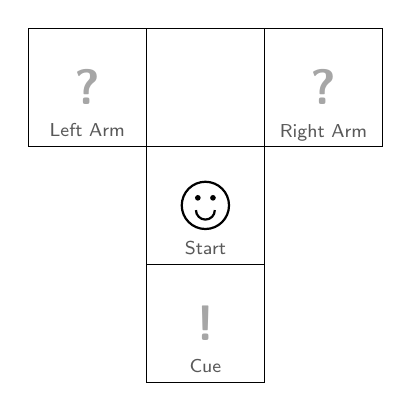
\begin{tikzpicture}[scale=1.5]
        \tikzset{
            agent/.pic={
                    \node[circle, draw=black, thick, fill=white, minimum size=0.5cm] at (0,0) {};
                    \fill[black] (-0.08, 0.08) circle (0.03);
                    \fill[black] (0.08, 0.08) circle (0.03);
                    \draw[thick] (-0.1, -0.05) arc (180:360:0.1);
                },
            field label/.style={
                    font=\tiny\sffamily, text=gray!70!black, anchor=south, scale=0.9, transform shape
                },
            field symbol/.style={
                    font=\large\bfseries,
                    text=gray!70,
                    anchor=center,
                    scale=1.0,
                    transform shape
                }
        }

        \draw (-0.5, 0) -- (-0.5, 2.0) -- (-1.5, 2.0) -- (-1.5, 3.0) -- (1.5, 3.0) -- (1.5, 2.0) -- (0.5, 2.0) -- (0.5, 0) -- cycle;
        \draw (-0.5, 1.0) -- (0.5, 1.0);
        \draw (-0.5, 2.0) -- (0.5, 2.0);
        \draw (-0.5, 2.0) -- (-0.5, 3.0);
        \draw (0.5, 2.0) -- (0.5, 3.0);

        \pic[scale=0.8, transform shape] at (0, 1.5) {agent};
        \node[field label] at (0, 0.97) {Start};
        \node[field label] at (0, -0.03) {Cue};
        \node[field label] at (-1.0, 1.97) {Left Arm};
        \node[field label] at (1.0, 1.93) {Right Arm};
        \node[field symbol] at (0, 0.5) {!};
        \node[field symbol] at (-1.0, 2.5) {?};
        \node[field symbol] at (1.0, 2.5) {?};
    \end{tikzpicture}

    \caption{The figure shows the T-Maze environment with its four fields (Left Arm, Right Arm, Start, and Cue) and the agent (Smiley) that is currently located at the start field. The empty space above the start field is not considered a field because the agent cannot move there.}
    \label{fig:27}
\end{figure}

The T-Maze environment is precisely discribed by a corresponding generative process that relates actions from the agent, hidden environmental states and observations generated by the environment probabilistically. Specifically, observations \(o\) are generated by (depend on) hidden environmental states \(s\) via the likelihood distribution \(p(o|s)\). Hidden environmental states evolve over time (from \(t\) to \(t+1\)) based on actions \(a\) via \(p(s_{t+1}|s_t, a_t)\). At timestep \(t=0\) hidden environmental states are given by the prior \(p(s_0)\). Before giving the probabilities of these relationships, I first define the observations, hidden states, and actions. Specifically, observations and hidden states can be defined as a cartesian product of three other sets. These sets are


\subsection{Parametrization}

Next, I assign concrete probabilities to the distributions of the generative process (of the T-Maze) and the generative models of the agents. There are large overlaps between the generative process and the generative models, which is why I give the concrete values here in a single place. However, it is important to realize that the generative process is in general not equal to the generative models of the agents. In the following I will first present the concrete events for which the distributions give probabilities. 
The events can be categorized into observations, (hidden) states, and actions. Regarding observations and hidden states, these can be defined as a cartesian product of three other sets. These sets are
\begin{equation}
    \text{Field} = \{\text{L}, \text{R}, \text{S}, \text{C}\},
\end{equation}
that defines the four fields (L (Left Arm), R (Right Arm), S (Start), C (Cue)) in the T-Maze,
\begin{equation}
    \text{MazeType} = \{\text{A}, \text{B}\},
\end{equation}
that defines the two possible types of the T-Maze, and
\begin{equation}
    \text{Outcome} = \{\text{RW}, \text{NR}, \text{CL}, \text{CR}\},
\end{equation}
that defines the four possible outcomes (not to be confused with observations) at a field (RW (Reward), NR (No Reward), CL (Cue hints at Left arm), CR (Cue hints at Right arm)).
Observations \(o \in O\) are defined as
\begin{alignat}{2}
    O =\; & \text{Field} \times \text{Outcome}                                                                                                                                             \nonumber \\
    =\;   & \{(\text{L},\text{RW}),(\text{L},\text{NR}),(\text{L},\text{CL}),(\text{L},\text{CR}),(\text{R},\text{RW}),(\text{R},\text{NR}),(\text{R},\text{CL}),(\text{R},\text{CR}),     \nonumber \\
          & \;\;(\text{S},\text{RW}),(\text{S},\text{NR}),(\text{S},\text{CL}),(\text{S},\text{CR}),(\text{C},\text{RW}),(\text{C},\text{NR}),(\text{C},\text{CL}),(\text{C},\text{CR})\},
\end{alignat}
hidden states \(s \in S\) (except for the context agents) are given by
\begin{alignat}{2}
    S =\; & \text{Field} \times \text{MazeType}                                                                                                                                  \nonumber \\
    =\;   & \{(\text{L},\text{A}),(\text{L},\text{B}),(\text{R},\text{A}),(\text{R},\text{B}),(\text{S},\text{A}),(\text{S},\text{B}),(\text{C},\text{A}),(\text{C},\text{B})\},
\end{alignat}
and actions \(a \in A\) are
\begin{equation}
    A = \{\text{GtL},\text{GtR},\text{GtS},\text{GtC}\},
\end{equation}
meaning GtL (Go to Left arm), GtR (Go to Right arm), GtS (Go to Start), and GtC (Go to Cue).

Next, it is important to notice that some parametrizations of distributions are shared among the generative process, the generative models of non-context agents (BFE- and GFE) and the generative models of context agents (Context-BFE- and Context-GFE). Following this, some definitions below refer to the generative process and/or multiple generative models (from non-context- and context agents). 
The initial hidden states \(s \in S\) at timestep \(k=0\) of the generative process (T-Maze) are randomly defined as
\begin{alignat}{1}
    p\bigl(s_0=(\text{S},\text{A})\bigr)=1
\end{alignat}
or
\begin{alignat}{1}
    p\bigl(s_0=(\text{S},\text{B})\bigr)=1,
\end{alignat}
i.e., at the beginning of a simulation the T-Maze type either assumes type A- or B. This is central to the information seeking mechanism of the GFE- and Context-GFE agents because they initially do not know the type and may seek information (about this) to find out.

Following this, the initial hidden states \(s \in S\) at timestep \(k=0\) of both non-context agents are defined as
\begin{alignat}{1}
    p\bigl(s_0=(\text{S},\text{A})\bigr)=p\bigl(s_0=(\text{S},\text{B})\bigr)=0.5.
\end{alignat}

The two context agents are equally uninformed but outsource the T-Maze type to their context states \(c \in \text{MazeType}\) with
\begin{alignat}{1}
    p\bigl(c=\text{A}\bigr)=p\bigl(c=\text{B}\bigr)=0.5.
\end{alignat}

Similarly to the non-context agents the context agents know that they are initially located at the start field via their hidden state \(s \in \text{Field}\) and
\begin{alignat}{1}
    p\bigl(s=\text{S}\bigr)=1.
\end{alignat}

The generative process and the non-context agents model the generation of observations \(o\) based on hidden states \(s \in S\) via
\begin{alignat}{3}
    & p\bigl(o=(\text{S},\text{CL})\bigm|s=(\text{S},\text{A})\bigr) &  & = p\bigl(o=(\text{S},\text{CL})\bigm|s=(\text{S},\text{B})\bigr) &  & = 0.5      \nonumber \\
    & p\bigl(o=(\text{S},\text{CR})\bigm|s=(\text{S},\text{A})\bigr) &  & = p\bigl(o=(\text{S},\text{CR})\bigm|s=(\text{S},\text{B})\bigr) &  & = 0.5      \nonumber \\
    & p\bigl(o=(\text{C},\text{CL})\bigm|s=(\text{C},\text{A})\bigr) &  & = p\bigl(o=(\text{C},\text{CR})\bigm|s=(\text{C},\text{B})\bigr) &  & = 1        \nonumber \\
    & p\bigl(o=(\text{L},\text{RW})\bigm|s=(\text{L},\text{A})\bigr) &  & = p\bigl(o=(\text{L},\text{NR})\bigm|s=(\text{L},\text{B})\bigr) &  & = \alpha   \nonumber \\
    & p\bigl(o=(\text{R},\text{RW})\bigm|s=(\text{R},\text{B})\bigr) &  & = p\bigl(o=(\text{R},\text{NR})\bigm|s=(\text{R},\text{A})\bigr) &  & = \alpha   \nonumber \\
    & p\bigl(o=(\text{L},\text{NR})\bigm|s=(\text{L},\text{B})\bigr) &  & = p\bigl(o=(\text{L},\text{RW})\bigm|s=(\text{L},\text{B})\bigr) &  & = 1-\alpha \nonumber \\
    & p\bigl(o=(\text{R},\text{NR})\bigm|s=(\text{R},\text{B})\bigr) &  & = p\bigl(o=(\text{R},\text{RW})\bigm|s=(\text{R},\text{A})\bigr) &  & = 1-\alpha,
\end{alignat}
where \(\alpha\) is a parameter that gets modulated in the simulations (explained below) and other probabilities \(p(o|s)\) are zero. 

In the case of the context agents the observations depend on both the hidden state \(s \in \text{Field}\) and the context state \(c \in \text{MazeType}\) via
\begin{alignat}{3}
    & p\bigl(o=(\text{S},\text{CL})\bigm|s=\text{S}, c=\text{A}\bigr) &  & = p\bigl(o=(\text{S},\text{CL})\bigm|s=\text{S}, c=\text{B}\bigr) &  & = 0.5      \nonumber \\
    & p\bigl(o=(\text{S},\text{CR})\bigm|s=\text{S}, c=\text{A}\bigr) &  & = p\bigl(o=(\text{S},\text{CR})\bigm|s=\text{S}, c=\text{B}\bigr) &  & = 0.5      \nonumber \\
    & p\bigl(o=(\text{C},\text{CL})\bigm|s=\text{C}, c=\text{A}\bigr) &  & = p\bigl(o=(\text{C},\text{CR})\bigm|s=\text{C}, c=\text{B}\bigr) &  & = 1        \nonumber \\
    & p\bigl(o=(\text{L},\text{RW})\bigm|s=\text{L}, c=\text{A}\bigr) &  & = p\bigl(o=(\text{L},\text{NR})\bigm|s=\text{L}, c=\text{B}\bigr) &  & = \alpha   \nonumber \\
    & p\bigl(o=(\text{R},\text{RW})\bigm|s=\text{R}, c=\text{B}\bigr) &  & = p\bigl(o=(\text{R},\text{NR})\bigm|s=\text{R}, c=\text{A}\bigr) &  & = \alpha   \nonumber \\
    & p\bigl(o=(\text{L},\text{NR})\bigm|s=\text{L}, c=\text{B}\bigr) &  & = p\bigl(o=(\text{L},\text{RW})\bigm|s=\text{L}, c=\text{B}\bigr) &  & = 1-\alpha \nonumber \\
    & p\bigl(o=(\text{R},\text{NR})\bigm|s=\text{R}, c=\text{B}\bigr) &  & = p\bigl(o=(\text{R},\text{RW})\bigm|s=\text{R}, c=\text{A}\bigr) &  & = 1-\alpha,
\end{alignat}
where other probabilities \(p(o|s,c)\) are zero. The parameter \(\alpha\) indicates how strongly the maze type is correlated with the reward location in the T-Maze. In the simulations the modulation of this parameter allows for a detailed analysis of the information seeking behavior of the GFE- and Context-GFE agents.

For both the generative process and the generative models of the non-context agents hidden states \(s_{k+1} \in S\) at time \(k+1\) depend on \(s_k \in S\) and actions \(a_k \in A\) at timestep \(k\) with probabilities
\begin{alignat}{3}
     & p\bigl(s_{k+1}=(\text{S},\text{A})\bigm|s_k=(\text{S},\text{A}),a_k=\text{GtS}\bigr) &  & =p\bigl(s_{k+1}=(\text{S},\text{B})\bigm|s_k=(\text{S},\text{B}),a_k=\text{GtS}\bigr) &  & = 1 \nonumber \\
     & p\bigl(s_{k+1}=(\text{C},\text{A})\bigm|s_k=(\text{S},\text{A}),a_k=\text{GtC}\bigr) &  & =p\bigl(s_{k+1}=(\text{C},\text{B})\bigm|s_k=(\text{S},\text{B}),a_k=\text{GtC}\bigr) &  & = 1 \nonumber \\
     & p\bigl(s_{k+1}=(\text{L},\text{A})\bigm|s_k=(\text{S},\text{A}),a_k=\text{GtL}\bigr) &  & =p\bigl(s_{k+1}=(\text{L},\text{B})\bigm|s_k=(\text{S},\text{B}),a_k=\text{GtL}\bigr) &  & = 1 \nonumber \\
     & p\bigl(s_{k+1}=(\text{R},\text{A})\bigm|s_k=(\text{S},\text{A}),a_k=\text{GtR}\bigr) &  & =p\bigl(s_{k+1}=(\text{R},\text{B})\bigm|s_k=(\text{S},\text{B}),a_k=\text{GtR}\bigr) &  & = 1 \nonumber \\[1.5em]
     & p\bigl(s_{k+1}=(\text{S},\text{A})\bigm|s_k=(\text{C},\text{A}),a_k=\text{GtS}\bigr) &  & =p\bigl(s_{k+1}=(\text{S},\text{B})\bigm|s_k=(\text{C},\text{B}),a_k=\text{GtS}\bigr) &  & = 1 \nonumber \\
     & p\bigl(s_{k+1}=(\text{C},\text{A})\bigm|s_k=(\text{C},\text{A}),a_k=\text{GtC}\bigr) &  & =p\bigl(s_{k+1}=(\text{C},\text{B})\bigm|s_k=(\text{C},\text{B}),a_k=\text{GtC}\bigr) &  & = 1 \nonumber \\
     & p\bigl(s_{k+1}=(\text{L},\text{A})\bigm|s_k=(\text{C},\text{A}),a_k=\text{GtL}\bigr) &  & =p\bigl(s_{k+1}=(\text{L},\text{B})\bigm|s_k=(\text{C},\text{B}),a_k=\text{GtL}\bigr) &  & = 1 \nonumber \\
     & p\bigl(s_{k+1}=(\text{R},\text{A})\bigm|s_k=(\text{C},\text{A}),a_k=\text{GtR}\bigr) &  & =p\bigl(s_{k+1}=(\text{R},\text{B})\bigm|s_k=(\text{C},\text{B}),a_k=\text{GtR}\bigr) &  & = 1 \nonumber \\[1.5em]
     & p\bigl(s_{k+1}=(\text{S},\text{A})\bigm|s_k=(\text{L},\text{A}),a_k=\text{GtS}\bigr) &  & =p\bigl(s_{k+1}=(\text{S},\text{B})\bigm|s_k=(\text{L},\text{B}),a_k=\text{GtS}\bigr) &  & = 1 \nonumber \\
     & p\bigl(s_{k+1}=(\text{S},\text{A})\bigm|s_k=(\text{L},\text{A}),a_k=\text{GtC}\bigr) &  & =p\bigl(s_{k+1}=(\text{S},\text{B})\bigm|s_k=(\text{L},\text{B}),a_k=\text{GtC}\bigr) &  & = 1 \nonumber \\
     & p\bigl(s_{k+1}=(\text{S},\text{A})\bigm|s_k=(\text{L},\text{A}),a_k=\text{GtL}\bigr) &  & =p\bigl(s_{k+1}=(\text{S},\text{B})\bigm|s_k=(\text{L},\text{B}),a_k=\text{GtL}\bigr) &  & = 1 \nonumber \\
     & p\bigl(s_{k+1}=(\text{S},\text{A})\bigm|s_k=(\text{L},\text{A}),a_k=\text{GtR}\bigr) &  & =p\bigl(s_{k+1}=(\text{S},\text{B})\bigm|s_k=(\text{L},\text{B}),a_k=\text{GtR}\bigr) &  & = 1 \nonumber \\[1.5em]
     & p\bigl(s_{k+1}=(\text{S},\text{A})\bigm|s_k=(\text{R},\text{A}),a_k=\text{GtS}\bigr) &  & =p\bigl(s_{k+1}=(\text{S},\text{B})\bigm|s_k=(\text{R},\text{B}),a_k=\text{GtS}\bigr) &  & = 1 \nonumber \\
     & p\bigl(s_{k+1}=(\text{S},\text{A})\bigm|s_k=(\text{R},\text{A}),a_k=\text{GtC}\bigr) &  & =p\bigl(s_{k+1}=(\text{S},\text{B})\bigm|s_k=(\text{R},\text{B}),a_k=\text{GtC}\bigr) &  & = 1 \nonumber \\
     & p\bigl(s_{k+1}=(\text{S},\text{A})\bigm|s_k=(\text{R},\text{A}),a_k=\text{GtL}\bigr) &  & =p\bigl(s_{k+1}=(\text{S},\text{B})\bigm|s_k=(\text{R},\text{B}),a_k=\text{GtL}\bigr) &  & = 1 \nonumber \\
     & p\bigl(s_{k+1}=(\text{S},\text{A})\bigm|s_k=(\text{R},\text{A}),a_k=\text{GtR}\bigr) &  & =p\bigl(s_{k+1}=(\text{S},\text{B})\bigm|s_k=(\text{R},\text{B}),a_k=\text{GtR}\bigr) &  & = 1
\end{alignat}
and other probabilities \(p(s_{k+1}|s_k,a_k)\) are zero.

Context agents have qualitatively equal transition probabilities for the hidden state \(s \in \text{Field}\) with
\begin{alignat}{3}
    & p\bigl(s_{k+1}=\text{S}\bigm|s_k=\text{S},a_k=\text{GtS}\bigr) &  & =p\bigl(s_{k+1}=\text{L}\bigm|s_k=\text{S},a_k=\text{GtL}\bigr) &  & = 1 \nonumber \\
    & p\bigl(s_{k+1}=\text{C}\bigm|s_k=\text{S},a_k=\text{GtC}\bigr) &  & =p\bigl(s_{k+1}=\text{R}\bigm|s_k=\text{S},a_k=\text{GtR}\bigr) &  & = 1 \nonumber \\
    & p\bigl(s_{k+1}=\text{S}\bigm|s_k=\text{C},a_k=\text{GtS}\bigr) &  & =p\bigl(s_{k+1}=\text{L}\bigm|s_k=\text{C},a_k=\text{GtL}\bigr) &  & = 1 \nonumber \\
    & p\bigl(s_{k+1}=\text{C}\bigm|s_k=\text{C},a_k=\text{GtC}\bigr) &  & =p\bigl(s_{k+1}=\text{R}\bigm|s_k=\text{C},a_k=\text{GtR}\bigr) &  & = 1 \nonumber \\
    & p\bigl(s_{k+1}=\text{S}\bigm|s_k=\text{L},a_k=\text{GtS}\bigr) &  & =p\bigl(s_{k+1}=\text{S}\bigm|s_k=\text{L},a_k=\text{GtL}\bigr) &  & = 1 \nonumber \\
    & p\bigl(s_{k+1}=\text{S}\bigm|s_k=\text{L},a_k=\text{GtC}\bigr) &  & =p\bigl(s_{k+1}=\text{S}\bigm|s_k=\text{L},a_k=\text{GtR}\bigr) &  & = 1 \nonumber \\
    & p\bigl(s_{k+1}=\text{S}\bigm|s_k=\text{R},a_k=\text{GtS}\bigr) &  & =p\bigl(s_{k+1}=\text{S}\bigm|s_k=\text{R},a_k=\text{GtL}\bigr) &  & = 1 \nonumber \\
    & p\bigl(s_{k+1}=\text{S}\bigm|s_k=\text{R},a_k=\text{GtC}\bigr) &  & =p\bigl(s_{k+1}=\text{S}\bigm|s_k=\text{R},a_k=\text{GtR}\bigr) &  & = 1
\end{alignat}
and other probabilities \(p(s_{k+1}|s_k,a_k)\) are zero.

The context state of context agents do not have a transition model like the hidden state \(s\), i.e., there is only a single context during a trial in the simulations.
All four agents have preferences for observations that are independent of the timestep. These preferences are the main drive in all agents that lead to purposeful behavior, i.e., acting to receive prefered observation. In the agents with information seeking these preferences compete with their curiousity. The preferences are defined via the parameter \(g\) in the goal distribution \(\tilde{p}(o)\):
\begin{alignat}{4}
    & \tilde{p}\bigl(o=(\text{L},\text{RW})\bigr) &  & =\tilde{p}\bigl(o=(\text{R},\text{RW})\bigr) &  & =\tilde{p}\bigl(o=(\text{S},\text{RW})\bigr) &  & =\tilde{p}\bigl(o=(\text{C},\text{RW})\bigr) \propto \exp(g) \nonumber \\
    & \tilde{p}\bigl(o=(\text{L},\text{NR})\bigr) &  & =\tilde{p}\bigl(o=(\text{R},\text{NR})\bigr) &  & =\tilde{p}\bigl(o=(\text{S},\text{NR})\bigr) &  & =\tilde{p}\bigl(o=(\text{C},\text{NR})\bigr) \propto \exp(-g)
\end{alignat}
After normalization, higher \(g\) values lead to stronger preferences for observing the reward (RW), weaker preferences for observing no reward (NR), and in between preferences for the remaining observations.

All agents also have a prior over actions that is also independent of the timestep. This prior is always defined as uniform distribution over all four actions:
\begin{alignat}{1}
    p(a=\text{GtL}) = p(a=\text{GtR}) = p(a=\text{GtS}) = p(a=\text{GtC}) = 0.25
\end{alignat}
In this way, the agents do not have biases for certain actions.


\subsection{Experiments}
\label{sec:simulations}

This section presents the schedule of the three experiments ("Initial Curiousity", "Exploiting Information", and "Long-Term Success"). Each simulation is run for each agent type ("BFE", "Context-BFE", "GFE", and "Context-GFE") and parameters \(\alpha \in [0.0, 0.1, \dots, 1.0]\) and \(c \in [0, 1, \dots, 10]\) of their generative models. The simulations reveal different aspects of the agents' behavior.
All simulations have in common that the agent begins in the start field of the T-Maze where it also initially receives an observation. This circumstance requires further explanation. First, the agent has a prior over its initial position in the T-Maze. This prior already entails the information that the agent begins at the start field, i.e., the agent already knows that it is located at this start field. Following this, the observation at this field does not yield any new information for the agent--the observation reveals to the agents its current location which the agent already "knows". Furthermore, this initial observation then has no effect on the agent, i.e., inferred actions are not dependent on this observation.

\subsubsection{Experiment 1: Initial Curiousity}

This experiment is designed to show the agents' initial drive to visit the cue location in the T-Maze. This is not to be understood as an empirical test, i.e., we do not have a cohort of the same agent type and average their behaviors. Instead, for each agent type the simulation is run once and their inclination of initially visiting the cue can directly be read of from their action specific belief distribution in the current timestep. Concretely, the respective agent first gets exposed to the environment (T-Maze) where it is initially located at the start position and the environment generates an observation that the agent perceives. Next, the agent performs inference, i.e., its message passing algorithm is executed until convergence. As a result, the agent has infered all of its belief distributions including the one that prescribes action in the current timestep. This action specific belief distribution contains probabilities over the four possible actions (go to (stay at) start, go to the left arm, go to the right arm, go to the cue). The agent's inclination of going to the cue is then exactly the respective probability of performing this action. This probability is the central result of this simulation. The procedere is exemplary detailed using the BFE agent in \cref{fig:24}.

\begin{figure}[htbp]
    \centering

    % ================= TIMESTEP 1 =================
    \begin{subfigure}[b]{\textwidth}
        \centering
        \fbox{%
            \begin{minipage}{0.97\linewidth}
                \vspace{0.15cm} % 1. Fester Abstand: OBEN
                % ==========================================
                % BEREICH 1: Das T-Maze (Flexibel zentriert)
                % ==========================================
                \hfill % Drückt das Maze von links weg
                \begin{tabular}{@{}c@{}}
                    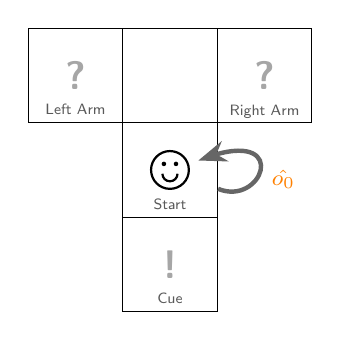
\begin{tikzpicture}[scale=1.2]
                        \tikzset{
                            agent/.pic={
                                    \node[circle, draw=black, thick, fill=white, minimum size=0.5cm] at (0,0) {};
                                    \fill[black] (-0.08, 0.08) circle (0.03);
                                    \fill[black] (0.08, 0.08) circle (0.03);
                                    \draw[thick] (-0.1, -0.05) arc (180:360:0.1);
                                },
                            field label/.style={
                                    font=\tiny\sffamily, text=gray!70!black, anchor=south, scale=0.9, transform shape
                                },
                            field symbol/.style={
                                    font=\large\bfseries,
                                    text=gray!70,
                                    anchor=center,
                                    scale=1.0,
                                    transform shape
                                }
                        }

                        \draw (-0.5, 0) -- (-0.5, 2.0) -- (-1.5, 2.0) -- (-1.5, 3.0) -- (1.5, 3.0) -- (1.5, 2.0) -- (0.5, 2.0) -- (0.5, 0) -- cycle;
                        \draw (-0.5, 1.0) -- (0.5, 1.0);
                        \draw (-0.5, 2.0) -- (0.5, 2.0);
                        \draw (-0.5, 2.0) -- (-0.5, 3.0);
                        \draw (0.5, 2.0) -- (0.5, 3.0);

                        \pic[scale=0.8, transform shape] at (0, 1.5) {agent};
                        % Observation Arrow
                        \draw[
                            -{Stealth[scale=1.0]},
                            line width=1.6pt,
                            color=gray!80!black
                        ]
                        (0.51, 1.3) .. controls (1.0, 1.1) and (1.3, 2.0) .. (0.3, 1.6);
                        \node[font=\footnotesize, text=gray!80!black] at (1.2, 1.4) {$\textcolor{orange}{\hat {o_0}}$};
                        \node[field label] at (0, 0.97) {Start};
                        \node[field label] at (0, -0.03) {Cue};
                        \node[field label] at (-1.0, 1.97) {Left Arm};
                        \node[field label] at (1.0, 1.93) {Right Arm};
                        \node[field symbol] at (0, 0.5) {!};
                        \node[field symbol] at (-1.0, 2.5) {?};
                        \node[field symbol] at (1.0, 2.5) {?};
                    \end{tikzpicture}
                \end{tabular}%
                \hfill % Drückt das Maze von der gestrichelten Linie weg (zentriert es somit perfekt im linken Rest-Raum)
                % ==========================================
                % BEREICH 2: Die Trennlinie
                % ==========================================
                \begin{tabular}{@{}c@{}}
                    \tikz \draw[dashed, thin, gray] (0,-2.1) -- (0,2.1);
                \end{tabular}%
                \hspace{0.3cm}% 2. Fester Abstand: LINKS VOM FFG
                % ==========================================
                % BEREICH 3: Der FFG (gibt die Breite vor)
                % ==========================================
                \begin{tabular}{@{}c@{}}
                    % Der FFG wird jetzt in seiner absolut natürlichen Größe gerendert.
                    \resizebox{9cm}{!}{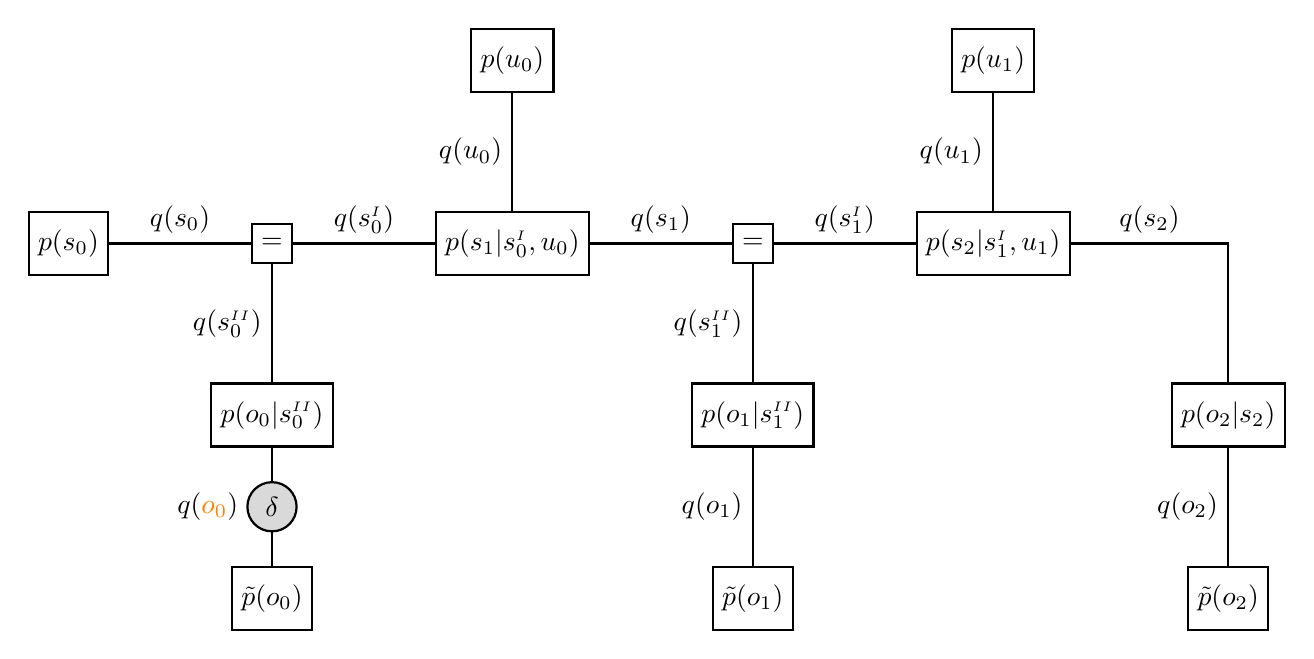
\begin{tikzpicture}[
    factor/.style={draw=black, thick, rectangle, minimum size=0.8cm, font=\normalsize},
    eqfactor/.style={draw=black, thick, rectangle, minimum size=0.5cm, font=\normalsize},
    edge/.style={thick},
    varlabel/.style={font=\normalsize},
    greycircle/.style={draw=black, thick, circle, fill=gray!30, minimum size=0.5cm, font=\normalsize}
]

% Knoten
\node[factor] (d) {$p(s_0)$};
\node[eqfactor, right=1.8cm of d] (eq0) {$=$};
\node[factor, below=1.5cm of eq0] (A0) {$p(o_0|s^{\scriptscriptstyle II}_0)$};
\node[factor, below=1.5cm of A0] (c0) {$\tilde{p}(o_0)$};
\node[factor, right=1.8cm of eq0] (B0) {$p(s_1|s^{\scriptscriptstyle I}_0,u_0)$};
\node[eqfactor, right=1.8cm of B0] (eq1) {$=$};
\node[factor, below=1.5cm of eq1] (A1) {$p(o_1|s^{\scriptscriptstyle II}_1)$};
\node[factor, below=1.5cm of A1] (c1) {$\tilde{p}(o_1)$};
\node[factor, right=1.8cm of eq1] (B1) {$p(s_2|s^{\scriptscriptstyle I}_1,u_1)$};
\node[factor] (A2) at ([xshift=2cm] B1.east |- A1) {$p(o_2|s_2)$};
\node[factor, below=1.5cm of A2] (c2) {$\tilde{p}(o_2)$};
\node[factor, above=1.5cm of B0] (u0) {$p(u_0)$};
\node[factor, above=1.5cm of B1] (u1) {$p(u_1)$};

% Kanten zwischen Knoten
\draw[edge] (d.east) -- (eq0.west) node[midway, above, varlabel] {$\textcolor{black}{q(s_0)}$};
\draw[edge] (eq0.south) -- (A0.north) node[midway, left, varlabel] {$\textcolor{black}{q(s^{\scriptscriptstyle II}_0)}$};
\draw[edge] (A0.south) -- (c0.north) node[midway, greycircle] {$\delta$} node[midway, left=0.3, varlabel] {$q(\textcolor{orange}{o_0})$};
\draw[edge] (eq0.east) -- (B0.west) node[midway, above, varlabel] {$\textcolor{black}{q(s^{\scriptscriptstyle I}_0)}$};
\draw[edge] (B0.north) -- (u0.south) node[midway, left, varlabel] {$\textcolor{black}{q(u_0)}$};
\draw[edge] (B0.east) -- (eq1.west) node[midway, above, varlabel] {$\textcolor{black}{q(s_1)}$};
\draw[edge] (eq1.south) -- (A1.north) node[midway, left, varlabel] {$\textcolor{black}{q(s^{\scriptscriptstyle II}_1)}$};
\draw[edge] (A1.south) -- (c1.north) node[midway, left, varlabel] {$\textcolor{black}{q(o_1)}$};
\draw[edge] (eq1.east) -- (B1.west) node[midway, above, varlabel] {$\textcolor{black}{q(s^{\scriptscriptstyle I}_1)}$};
\draw[edge] (B1.east) -| (A2.north) node[pos=0.25, above, varlabel] {$\textcolor{black}{q(s_2)}$};
\draw[edge] (A2.south) -- (c2.north) node[midway, left, varlabel] {$\textcolor{black}{q(o_2)}$};
\draw[edge] (B1.north) -- (u1.south) node[midway, left, varlabel] {$\textcolor{black}{q(u_1)}$};

\end{tikzpicture}}
                \end{tabular}%
                \llap{\smash{\raisebox{2.0cm}[0pt][0pt]{\sffamily\bfseries\small (a)\hspace*{-0.0cm}}}}%
                \hspace{0.1cm}% 3. Fester Abstand: RECHTS VOM FFG (Zum Box-Rand)
                \vspace{0.02cm} % 4. Fester Abstand: UNTEN
            \end{minipage}%
        }
        \phantomcaption
        \label{fig:24.1}
    \end{subfigure}

    \vspace{0.2cm} % Abstand zwischen den Kästen

    % ================= TIMESTEP 1 =================
    \begin{subfigure}[b]{\textwidth}
        \centering
        \fbox{%
            \begin{minipage}{0.97\linewidth}
                \vspace{0.15cm} % 1. Fester Abstand: OBEN
                % ==========================================
                % BEREICH 1: Das T-Maze (Flexibel zentriert)
                % ==========================================
                \hfill % Drückt das Maze von links weg
                \begin{tabular}{@{}c@{}}
                    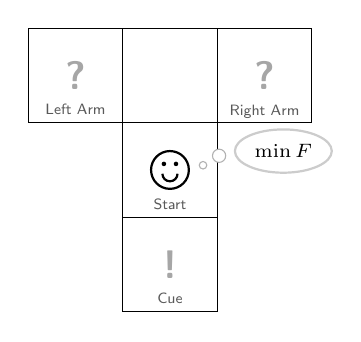
\begin{tikzpicture}[scale=1.2]
                        \tikzset{
                            agent/.pic={
                                    \node[circle, draw=black, thick, fill=white, minimum size=0.5cm] at (0,0) {};
                                    \fill[black] (-0.08, 0.08) circle (0.03);
                                    \fill[black] (0.08, 0.08) circle (0.03);
                                    \draw[thick] (-0.1, -0.05) arc (180:360:0.1);
                                },
                            field label/.style={
                                    font=\tiny\sffamily, text=gray!70!black, anchor=south, scale=0.9, transform shape
                                },
                            field symbol/.style={
                                    font=\large\bfseries,
                                    text=gray!70,
                                    anchor=center,
                                    scale=1.0,
                                    transform shape
                                }
                        }

                        \draw (-0.5, 0) -- (-0.5, 2.0) -- (-1.5, 2.0) -- (-1.5, 3.0) -- (1.5, 3.0) -- (1.5, 2.0) -- (0.5, 2.0) -- (0.5, 0) -- cycle;
                        \draw (-0.5, 1.0) -- (0.5, 1.0);
                        \draw (-0.5, 2.0) -- (0.5, 2.0);
                        \draw (-0.5, 2.0) -- (-0.5, 3.0);
                        \draw (0.5, 2.0) -- (0.5, 3.0);

                        \pic[scale=0.8, transform shape] at (0, 1.5) {agent};
                        \node[field label] at (0, 0.97) {Start};
                        \node[field label] at (0, -0.03) {Cue};
                        \node[field label] at (-1.0, 1.97) {Left Arm};
                        \node[field label] at (1.0, 1.93) {Right Arm};
                        \node[field symbol] at (0, 0.5) {!};
                        \node[field symbol] at (-1.0, 2.5) {?};
                        \node[field symbol] at (1.0, 2.5) {?};

                        % --- NEU: Gedankenblase für Variational Free Energy Minimierung ---
                        % Kleine Bläschen, die vom Kopf (ca. 0.3, 1.7) nach rechts oben steigen
                        \draw[thin, gray!60, fill=white] (0.35, 1.55) circle (0.04);
                        \draw[thin, gray!60, fill=white] (0.52, 1.65) circle (0.07);

                        % Die Haupt-Gedankenblase mit dem Minimierungs-Symbol / Free Energy F
                        \node[
                            ellipse,
                            draw=gray!40,
                            thick,
                            fill=white,
                            minimum width=1.0cm,
                            minimum height=0.55cm,
                            inner sep=2pt,
                            font=\scriptsize\sffamily,
                            text=black!100!black
                        ] at (1.2, 1.7) {$\min F$};
                    \end{tikzpicture}
                \end{tabular}%
                \hfill % Drückt das Maze von der gestrichelten Linie weg (zentriert es somit perfekt im linken Rest-Raum)
                % ==========================================
                % BEREICH 2: Die Trennlinie
                % ==========================================
                \begin{tabular}{@{}c@{}}
                    \tikz \draw[dashed, thin, gray] (0,-2.1) -- (0,2.1);
                \end{tabular}%
                \hspace{0.3cm}% 2. Fester Abstand: LINKS VOM FFG
                % ==========================================
                % BEREICH 3: Der FFG (gibt die Breite vor)
                % ==========================================
                \begin{tabular}{@{}c@{}}
                    % Der FFG wird jetzt in seiner absolut natürlichen Größe gerendert.
                    \resizebox{9cm}{!}{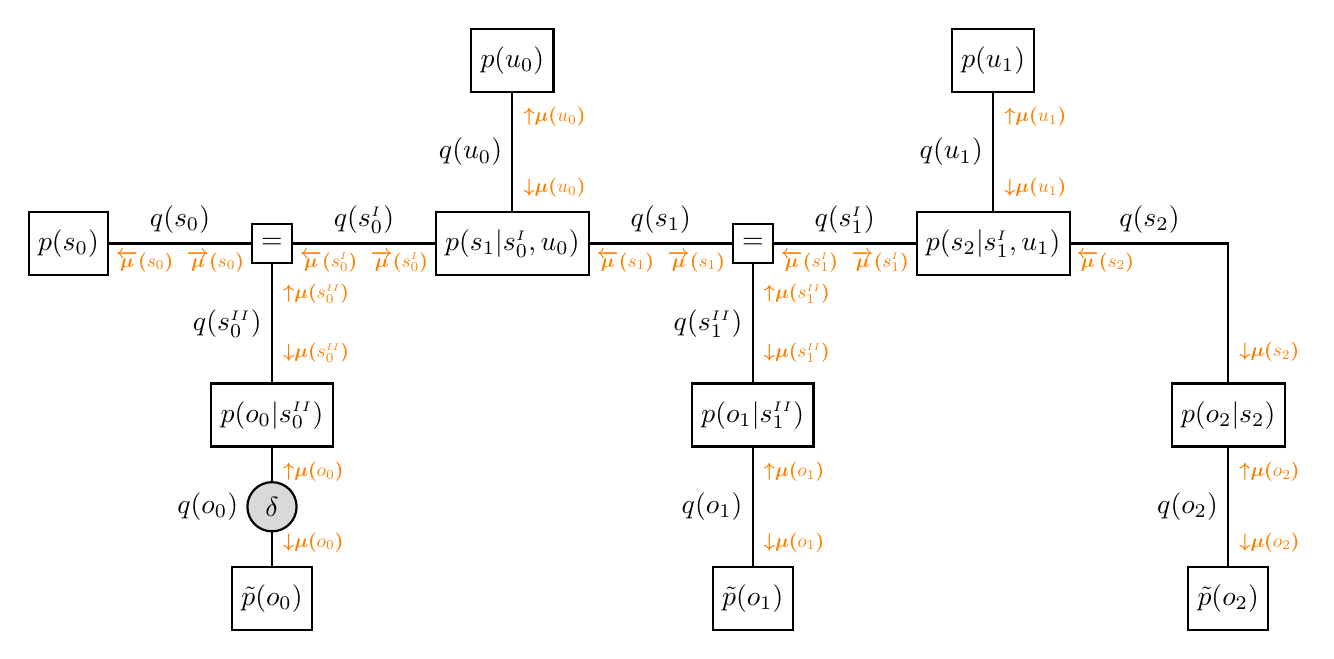
\begin{tikzpicture}[
    factor/.style={draw=black, thick, rectangle, minimum size=0.8cm, font=\normalsize},
    eqfactor/.style={draw=black, thick, rectangle, minimum size=0.5cm, font=\normalsize},
    edge/.style={thick},
    varlabel/.style={font=\normalsize},
    greycircle/.style={draw=black, thick, circle, fill=gray!30, minimum size=0.5cm, font=\normalsize}
]

% Knoten
\node[factor] (d) {$p(s_0)$};
\node[eqfactor, right=1.8cm of d] (eq0) {$=$};
\node[factor, below=1.5cm of eq0] (A0) {$p(o_0|s^{\scriptscriptstyle II}_0)$};
\node[factor, below=1.5cm of A0] (c0) {$\tilde{p}(o_0)$};
\node[factor, right=1.8cm of eq0] (B0) {$p(s_1|s^{\scriptscriptstyle I}_0,u_0)$};
\node[eqfactor, right=1.8cm of B0] (eq1) {$=$};
\node[factor, below=1.5cm of eq1] (A1) {$p(o_1|s^{\scriptscriptstyle II}_1)$};
\node[factor, below=1.5cm of A1] (c1) {$\tilde{p}(o_1)$};
\node[factor, right=1.8cm of eq1] (B1) {$p(s_2|s^{\scriptscriptstyle I}_1,u_1)$};
\node[factor] (A2) at ([xshift=2cm] B1.east |- A1) {$p(o_2|s_2)$};
\node[factor, below=1.5cm of A2] (c2) {$\tilde{p}(o_2)$};
\node[factor, above=1.5cm of B0] (u0) {$p(u_0)$};
\node[factor, above=1.5cm of B1] (u1) {$p(u_1)$};

% Kanten zwischen Knoten
\draw[edge] (d.east) -- (eq0.west) node[midway, above, varlabel] {$\textcolor{black}{q(s_0)}$} node[near end, below, varlabel, scale=0.7] {$\textcolor{orange}{\bm{\overrightarrow{\mu}(}s_0\bm{)}}$} node[near start, below, varlabel, scale=0.7] {$\textcolor{orange}{\bm{\overleftarrow{\mu}(}s_0\bm{)}}$};
\draw[edge] (eq0.south) -- (A0.north) node[midway, left, varlabel] {$\textcolor{black}{q(s^{\scriptscriptstyle II}_0)}$} node[pos=0.25, right=0.05, varlabel, scale=0.7] {$\textcolor{orange}{\bm{{\uparrow}{\mu}(}s^{\scriptscriptstyle II}_0\bm{)}}$} node[pos=0.75, right=0.05, varlabel, scale=0.7] {$\textcolor{orange}{\bm{{\downarrow}{\mu}(}s^{\scriptscriptstyle II}_0\bm{)}}$};
\draw[edge] (A0.south) -- (c0.north) node[midway, greycircle] {$\delta$} node[midway, left=0.3, varlabel] {$\textcolor{black}{q(o_0)}$} node[pos=0.2, right=0.05, varlabel, scale=0.7] {$\textcolor{orange}{\bm{{\uparrow}{\mu}(}o_0\bm{)}}$} node[pos=0.8, right=0.05, varlabel, scale=0.7] {$\textcolor{orange}{\bm{{\downarrow}{\mu}(}o_0\bm{)}}$};
\draw[edge] (eq0.east) -- (B0.west) node[midway, above, varlabel] {$\textcolor{black}{q(s^{\scriptscriptstyle I}_0)}$} node[near start, below, varlabel, scale=0.7] {$\textcolor{orange}{\bm{\overleftarrow{\mu}(}s^{\scriptscriptstyle I}_0\bm{)}}$} node[near end, below, varlabel, scale=0.7] {$\textcolor{orange}{\bm{\overrightarrow{\mu}(}s^{\scriptscriptstyle I}_0\bm{)}}$};
\draw[edge] (B0.north) -- (u0.south) node[midway, left, varlabel] {$\textcolor{black}{q(u_0)}$} node[pos=0.2, right=0.05, varlabel, scale=0.7] {$\textcolor{orange}{\bm{{\downarrow}{\mu}(}u_0\bm{)}}$} node[pos=0.8, right=0.05, varlabel, scale=0.7] {$\textcolor{orange}{\bm{{\uparrow}{\mu}(}u_0\bm{)}}$};
\draw[edge] (B0.east) -- (eq1.west) node[midway, above, varlabel] {$\textcolor{black}{q(s_1)}$} node[near end, below, varlabel, scale=0.7] {$\textcolor{orange}{\bm{\overrightarrow{\mu}(}s_1\bm{)}}$} node[near start, below, varlabel, scale=0.7] {$\textcolor{orange}{\bm{\overleftarrow{\mu}(}s_1\bm{)}}$};
\draw[edge] (eq1.south) -- (A1.north) node[midway, left, varlabel] {$\textcolor{black}{q(s^{\scriptscriptstyle II}_1)}$} node[pos=0.25, right=0.05, varlabel, scale=0.7] {$\textcolor{orange}{\bm{{\uparrow}{\mu}(}s^{\scriptscriptstyle II}_1\bm{)}}$} node[pos=0.75, right=0.05, varlabel, scale=0.7] {$\textcolor{orange}{\bm{{\downarrow}{\mu}(}s^{\scriptscriptstyle II}_1\bm{)}}$};
\draw[edge] (A1.south) -- (c1.north) node[midway, left, varlabel] {$\textcolor{black}{q(o_1)}$} node[pos=0.2, right=0.05, varlabel, scale=0.7] {$\textcolor{orange}{\bm{{\uparrow}{\mu}(}o_1\bm{)}}$} node[pos=0.8, right=0.05, varlabel, scale=0.7] {$\textcolor{orange}{\bm{{\downarrow}{\mu}(}o_1\bm{)}}$};
\draw[edge] (eq1.east) -- (B1.west) node[midway, above, varlabel] {$\textcolor{black}{q(s^{\scriptscriptstyle I}_1)}$} node[near start, below, varlabel, scale=0.7] {$\textcolor{orange}{\bm{\overleftarrow{\mu}(}s^{\scriptscriptstyle I}_1\bm{)}}$} node[near end, below, varlabel, scale=0.7] {$\textcolor{orange}{\bm{\overrightarrow{\mu}(}s^{\scriptscriptstyle I}_1\bm{)}}$};
\draw[edge] (B1.east) -| (A2.north) node[pos=0.25, above, varlabel] {$\textcolor{black}{q(s_2)}$} node[pos=0.89, right=0.05, varlabel, scale=0.7] {$\textcolor{orange}{\bm{{\downarrow}{\mu}(}s_2\bm{)}}$} node[pos=0.11, below, varlabel, scale=0.7] {$\textcolor{orange}{\bm{\overleftarrow{\mu}(}s_2\bm{)}}$};
\draw[edge] (A2.south) -- (c2.north) node[midway, left, varlabel] {$\textcolor{black}{q(o_2)}$} node[pos=0.2, right=0.05, varlabel, scale=0.7] {$\textcolor{orange}{\bm{{\uparrow}{\mu}(}o_2\bm{)}}$} node[pos=0.8, right=0.05, varlabel, scale=0.7] {$\textcolor{orange}{\bm{{\downarrow}{\mu}(}o_2\bm{)}}$};
\draw[edge] (B1.north) -- (u1.south) node[midway, left, varlabel] {$\textcolor{black}{q(u_1)}$} node[pos=0.2, right=0.05, varlabel, scale=0.7] {$\textcolor{orange}{\bm{{\downarrow}{\mu}(}u_1\bm{)}}$} node[pos=0.8, right=0.05, varlabel, scale=0.7] {$\textcolor{orange}{\bm{{\uparrow}{\mu}(}u_1\bm{)}}$};

\end{tikzpicture}}
                \end{tabular}%
                \llap{\smash{\raisebox{2.0cm}[0pt][0pt]{\sffamily\bfseries\small (b)\hspace*{-0.0cm}}}}%
                \hspace{0.1cm}% 3. Fester Abstand: RECHTS VOM FFG (Zum Box-Rand)
                \vspace{0.02cm} % 4. Fester Abstand: UNTEN
            \end{minipage}%
        }
        \phantomcaption
        \label{fig:24.2}
    \end{subfigure}

    \caption{The figure presents the two crucial steps of the "Initial Curiousity" simulation using the example of the BFE agent: First, the agent receives an observation \(\hat {o_0}\) from the environment (\cref{fig:24.1}). The observation has an effect on the agent's temporal generative model, i.e., in its factor graph representation, the belief distribution \(q(o_0)\) that describes its belief about observations of timestep \(t=0\), becomes a delta distribution with all probability mass at \(\hat {o_0}\). Second, the agent performs inference, i.e., it runs its message passing algorithm (messages sent along the edges in \cref{fig:24.2}). In the case of the BFE agent this refers to \cref{alg:2}. After message passing has finished, the beliefs of executing a certain action in the current timestep are then directly given by the belief \(q(u_0)\).}
    \label{fig:24}
\end{figure}


\subsubsection{Experiment 2: Exploiting Information}

In this experiment, the agent receives the cue which reveals the location of the reward (left arm or right arm) in the T-Maze. The result of this experiment is then the agent's inclination of going to the respective arm in the T-Maze that the cue indicates as given by the probabilities in its action-specific belief distribution. The simulation spans over timesteps \(t=0\) and \(t=1\). First, the agent receives an observation \(o_0\) generated be the environment (at \(t=0\)). Second, it executes the "go to cue" action and thus moves to the cue field in the environment, i.e., the action is not sampled from the action belief distribution \(q(u_0)\) but is externally triggered (at \(t=0\)). Third, it receives the second observation \(o_1\) while being at the cue field (at \(t=1\)). Fourth, the agent runs its messages passing algorithm to infer its belief distributions. After inference, the result of the experiment is given as the agent's belief (a probability) of executing the specific action that moves it to the arm that is indicated by the cue. A detailed explanation of the procedere is given in \cref{fig:25}.

\begin{figure}[bp!]
    \centering
    \resizebox{1.0\textwidth}{!}{%
        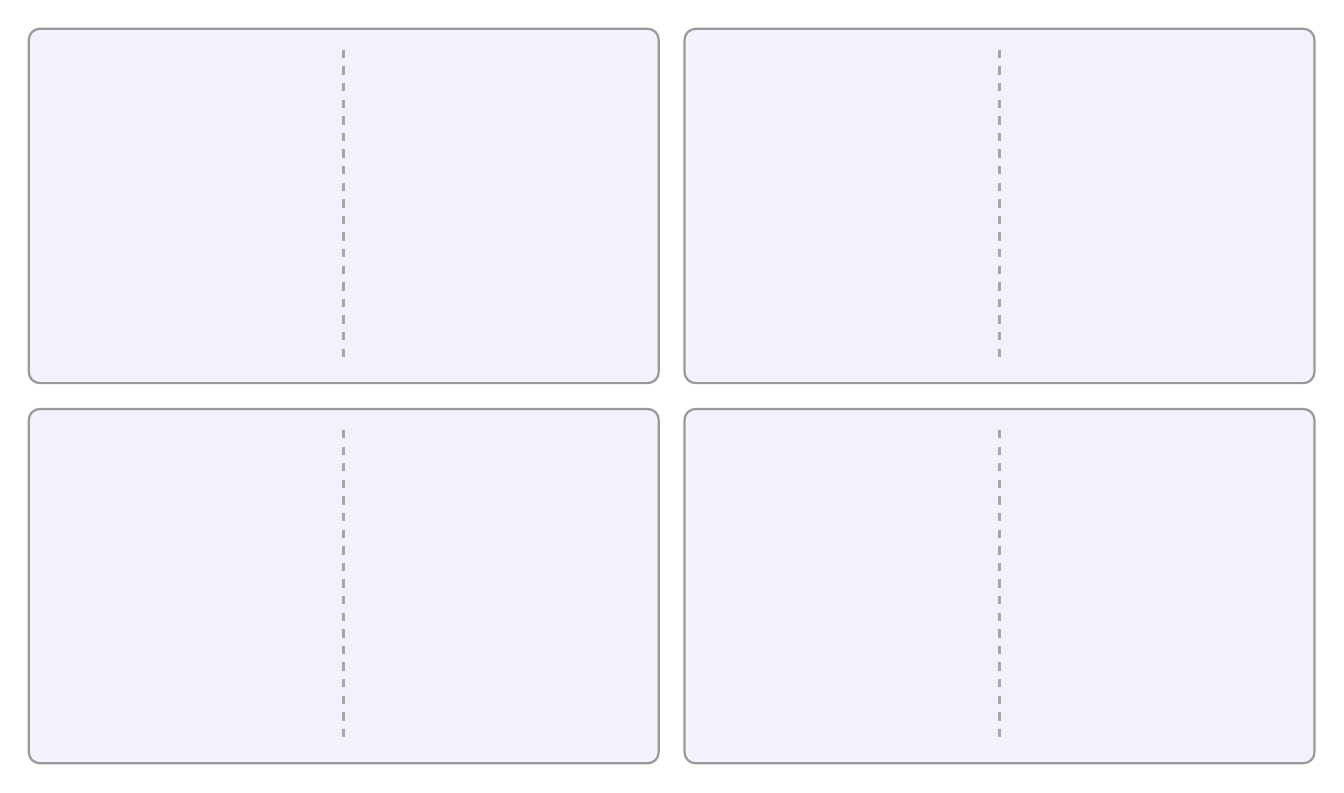
\begin{tikzpicture}[
                panel/.style={
                    draw=gray!80, thick, fill=blue!5,
                    rounded corners=4pt,
                    minimum width=8.0cm,
                    minimum height=4.5cm,
                    inner sep=0pt,
                    align=center
                },
                sublabel/.style={
                    anchor=north east,
                    font=\sffamily\bfseries\Large,
                    text=black
                },
                divider/.style={
                    draw=gray!70,
                    dashed,
                    line width=1.0pt
                }
            ]

            % --- 2x2 Grid (Feste Positionierung) ---
            % Obere Reihe: (a) und (b)
            \node[panel] (boxA) at (0,0) {
                % \usebox{\boxA}
            };

            \node[panel, right=0.3cm of boxA] (boxB) {
                % \usebox{\boxB}
            };

            % Untere Reihe: (c) und (d)
            \node[panel, below=0.3cm of boxA] (boxC) {
                % \usebox{\boxC}
            };

            \node[panel, right=0.3cm of boxC] (boxD) {
                % \usebox{\boxD}
            };

            \foreach \b in {boxA, boxB, boxC, boxD} {
                % yshift sorgt für einen kleinen Abstand zum oberen/unteren Rand
                \draw[divider] ([yshift=-8pt]\b.north) -- ([yshift=8pt]\b.south);
            }

            % --- Labels (a), (b), (c), (d) fix oben rechts verankert ---
            %\node[sublabel] at ([xshift=-10pt, yshift=-8pt]boxA.north east) {(a)};
            %\node[sublabel] at ([xshift=-10pt, yshift=-8pt]boxB.north east) {(b)};
            %\node[sublabel] at ([xshift=-10pt, yshift=-8pt]boxC.north east) {(c)};
            %\node[sublabel] at ([xshift=-10pt, yshift=-8pt]boxD.north east) {(d)};

        \end{tikzpicture}
    }
    \caption{Overview of the four experimental setups: (a) initial curiosity, (b) belief state, (c) free energy minimization during planning, and (d) action execution.}
    \label{fig:four_panels}
\end{figure}

\begin{figure}[b!]
    \centering

    % ================= TIMESTEP 1 =================
    \begin{subfigure}[b]{\textwidth}
        \centering
        \fbox{%
            \begin{minipage}{0.97\linewidth}
                \vspace{0.15cm} % 1. Fester Abstand: OBEN
                % ==========================================
                % BEREICH 1: Das T-Maze (Flexibel zentriert)
                % ==========================================
                \hfill % Drückt das Maze von links weg
                \begin{tabular}{@{}c@{}}
                    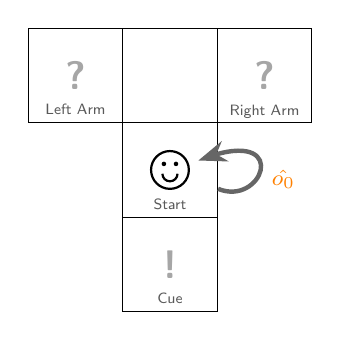
\begin{tikzpicture}[scale=1.2]
                        \tikzset{
                            agent/.pic={
                                    \node[circle, draw=black, thick, fill=white, minimum size=0.5cm] at (0,0) {};
                                    \fill[black] (-0.08, 0.08) circle (0.03);
                                    \fill[black] (0.08, 0.08) circle (0.03);
                                    \draw[thick] (-0.1, -0.05) arc (180:360:0.1);
                                },
                            field label/.style={
                                    font=\tiny\sffamily, text=gray!70!black, anchor=south, scale=0.9, transform shape
                                },
                            field symbol/.style={
                                    font=\large\bfseries,
                                    text=gray!70,
                                    anchor=center,
                                    scale=1.0,
                                    transform shape
                                }
                        }

                        \draw (-0.5, 0) -- (-0.5, 2.0) -- (-1.5, 2.0) -- (-1.5, 3.0) -- (1.5, 3.0) -- (1.5, 2.0) -- (0.5, 2.0) -- (0.5, 0) -- cycle;
                        \draw (-0.5, 1.0) -- (0.5, 1.0);
                        \draw (-0.5, 2.0) -- (0.5, 2.0);
                        \draw (-0.5, 2.0) -- (-0.5, 3.0);
                        \draw (0.5, 2.0) -- (0.5, 3.0);

                        \pic[scale=0.8, transform shape] at (0, 1.5) {agent};
                        % Observation Arrow
                        \draw[
                            -{Stealth[scale=1.0]},
                            line width=1.6pt,
                            color=gray!80!black
                        ]
                        (0.51, 1.3) .. controls (1.0, 1.1) and (1.3, 2.0) .. (0.3, 1.6);
                        \node[font=\footnotesize, text=gray!80!black] at (1.2, 1.4) {$\textcolor{orange}{\hat {o_0}}$};
                        \node[field label] at (0, 0.97) {Start};
                        \node[field label] at (0, -0.03) {Cue};
                        \node[field label] at (-1.0, 1.97) {Left Arm};
                        \node[field label] at (1.0, 1.93) {Right Arm};
                        \node[field symbol] at (0, 0.5) {!};
                        \node[field symbol] at (-1.0, 2.5) {?};
                        \node[field symbol] at (1.0, 2.5) {?};
                    \end{tikzpicture}
                \end{tabular}%
                \hfill % Drückt das Maze von der gestrichelten Linie weg (zentriert es somit perfekt im linken Rest-Raum)
                % ==========================================
                % BEREICH 2: Die Trennlinie
                % ==========================================
                \begin{tabular}{@{}c@{}}
                    \tikz \draw[dashed, thin, gray] (0,-2.1) -- (0,2.1);
                \end{tabular}%
                \hspace{0.3cm}% 2. Fester Abstand: LINKS VOM FFG
                % ==========================================
                % BEREICH 3: Der FFG (gibt die Breite vor)
                % ==========================================
                \begin{tabular}{@{}c@{}}
                    % Der FFG wird jetzt in seiner absolut natürlichen Größe gerendert.
                    \resizebox{9cm}{!}{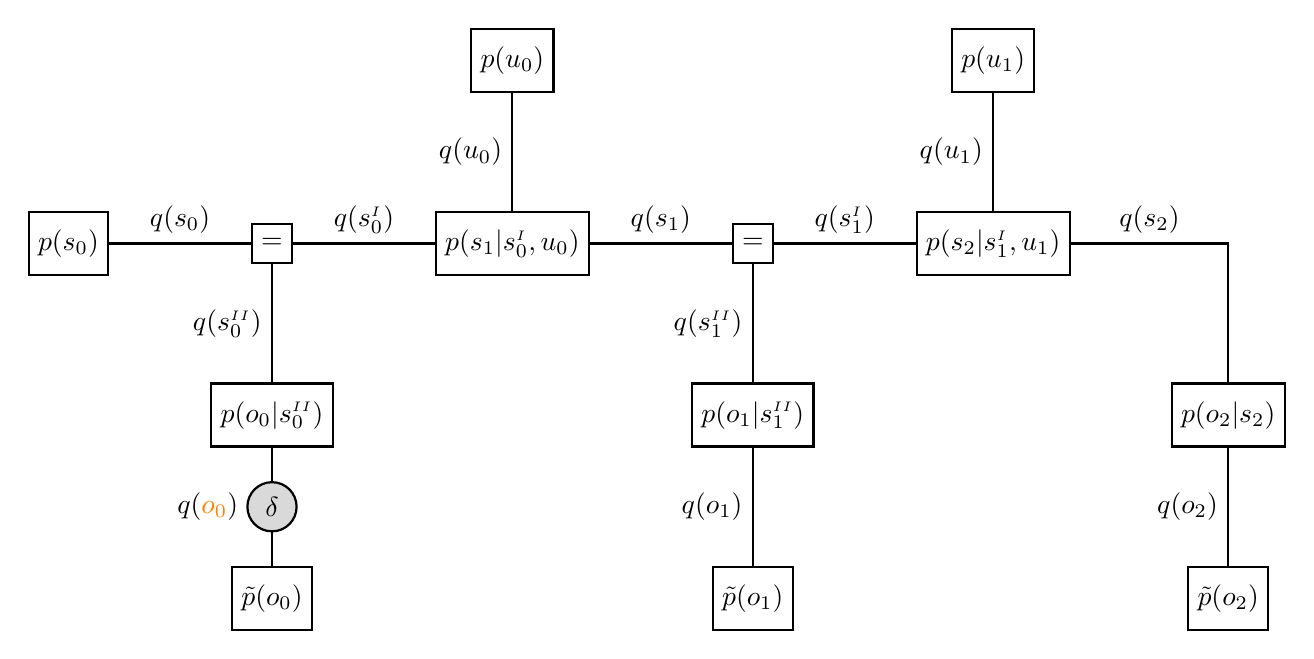
\begin{tikzpicture}[
    factor/.style={draw=black, thick, rectangle, minimum size=0.8cm, font=\normalsize},
    eqfactor/.style={draw=black, thick, rectangle, minimum size=0.5cm, font=\normalsize},
    edge/.style={thick},
    varlabel/.style={font=\normalsize},
    greycircle/.style={draw=black, thick, circle, fill=gray!30, minimum size=0.5cm, font=\normalsize}
]

% Knoten
\node[factor] (d) {$p(s_0)$};
\node[eqfactor, right=1.8cm of d] (eq0) {$=$};
\node[factor, below=1.5cm of eq0] (A0) {$p(o_0|s^{\scriptscriptstyle II}_0)$};
\node[factor, below=1.5cm of A0] (c0) {$\tilde{p}(o_0)$};
\node[factor, right=1.8cm of eq0] (B0) {$p(s_1|s^{\scriptscriptstyle I}_0,u_0)$};
\node[eqfactor, right=1.8cm of B0] (eq1) {$=$};
\node[factor, below=1.5cm of eq1] (A1) {$p(o_1|s^{\scriptscriptstyle II}_1)$};
\node[factor, below=1.5cm of A1] (c1) {$\tilde{p}(o_1)$};
\node[factor, right=1.8cm of eq1] (B1) {$p(s_2|s^{\scriptscriptstyle I}_1,u_1)$};
\node[factor] (A2) at ([xshift=2cm] B1.east |- A1) {$p(o_2|s_2)$};
\node[factor, below=1.5cm of A2] (c2) {$\tilde{p}(o_2)$};
\node[factor, above=1.5cm of B0] (u0) {$p(u_0)$};
\node[factor, above=1.5cm of B1] (u1) {$p(u_1)$};

% Kanten zwischen Knoten
\draw[edge] (d.east) -- (eq0.west) node[midway, above, varlabel] {$\textcolor{black}{q(s_0)}$};
\draw[edge] (eq0.south) -- (A0.north) node[midway, left, varlabel] {$\textcolor{black}{q(s^{\scriptscriptstyle II}_0)}$};
\draw[edge] (A0.south) -- (c0.north) node[midway, greycircle] {$\delta$} node[midway, left=0.3, varlabel] {$q(\textcolor{orange}{o_0})$};
\draw[edge] (eq0.east) -- (B0.west) node[midway, above, varlabel] {$\textcolor{black}{q(s^{\scriptscriptstyle I}_0)}$};
\draw[edge] (B0.north) -- (u0.south) node[midway, left, varlabel] {$\textcolor{black}{q(u_0)}$};
\draw[edge] (B0.east) -- (eq1.west) node[midway, above, varlabel] {$\textcolor{black}{q(s_1)}$};
\draw[edge] (eq1.south) -- (A1.north) node[midway, left, varlabel] {$\textcolor{black}{q(s^{\scriptscriptstyle II}_1)}$};
\draw[edge] (A1.south) -- (c1.north) node[midway, left, varlabel] {$\textcolor{black}{q(o_1)}$};
\draw[edge] (eq1.east) -- (B1.west) node[midway, above, varlabel] {$\textcolor{black}{q(s^{\scriptscriptstyle I}_1)}$};
\draw[edge] (B1.east) -| (A2.north) node[pos=0.25, above, varlabel] {$\textcolor{black}{q(s_2)}$};
\draw[edge] (A2.south) -- (c2.north) node[midway, left, varlabel] {$\textcolor{black}{q(o_2)}$};
\draw[edge] (B1.north) -- (u1.south) node[midway, left, varlabel] {$\textcolor{black}{q(u_1)}$};

\end{tikzpicture}}
                \end{tabular}%
                \llap{\smash{\raisebox{2.0cm}[0pt][0pt]{\sffamily\bfseries\small (a)\hspace*{-0.0cm}}}}%
                \hspace{0.1cm}% 3. Fester Abstand: RECHTS VOM FFG (Zum Box-Rand)
                \vspace{0.02cm} % 4. Fester Abstand: UNTEN
            \end{minipage}%
        }
        \phantomcaption
        \label{fig:25.1}
    \end{subfigure}

    \vspace{0.2cm} % Abstand zwischen den Kästen

    % ================= TIMESTEP 1 =================
    \begin{subfigure}[b]{\textwidth}
        \centering
        \fbox{%
            \begin{minipage}{0.97\linewidth}
                \vspace{0.15cm} % 1. Fester Abstand: OBEN
                % ==========================================
                % BEREICH 1: Das T-Maze (Flexibel zentriert)
                % ==========================================
                \hfill % Drückt das Maze von links weg
                \begin{tabular}{@{}c@{}}
                    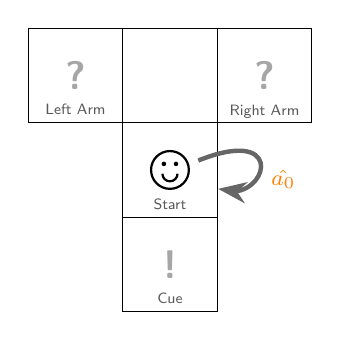
\begin{tikzpicture}[scale=1.2]
                        \tikzset{
                            agent/.pic={
                                    \node[circle, draw=black, thick, fill=white, minimum size=0.5cm] at (0,0) {};
                                    \fill[black] (-0.08, 0.08) circle (0.03);
                                    \fill[black] (0.08, 0.08) circle (0.03);
                                    \draw[thick] (-0.1, -0.05) arc (180:360:0.1);
                                },
                            field label/.style={
                                    font=\tiny\sffamily, text=gray!70!black, anchor=south, scale=0.9, transform shape
                                },
                            field symbol/.style={
                                    font=\large\bfseries,
                                    text=gray!70,
                                    anchor=center,
                                    scale=1.0,
                                    transform shape
                                }
                        }

                        \draw (-0.5, 0) -- (-0.5, 2.0) -- (-1.5, 2.0) -- (-1.5, 3.0) -- (1.5, 3.0) -- (1.5, 2.0) -- (0.5, 2.0) -- (0.5, 0) -- cycle;
                        \draw (-0.5, 1.0) -- (0.5, 1.0);
                        \draw (-0.5, 2.0) -- (0.5, 2.0);
                        \draw (-0.5, 2.0) -- (-0.5, 3.0);
                        \draw (0.5, 2.0) -- (0.5, 3.0);

                        \pic[scale=0.8, transform shape] at (0, 1.5) {agent};
                        % Observation Arrow
                        \draw[
                            {Stealth[scale=1.0]}-,
                            line width=1.6pt,
                            color=gray!80!black
                        ]
                        (0.51, 1.3) .. controls (1.0, 1.1) and (1.3, 2.0) .. (0.3, 1.6);
                        \node[font=\footnotesize, text=gray!80!black] at (1.2, 1.4) {$\textcolor{orange}{\hat {a_0}}$};
                        \node[field label] at (0, 0.97) {Start};
                        \node[field label] at (0, -0.03) {Cue};
                        \node[field label] at (-1.0, 1.97) {Left Arm};
                        \node[field label] at (1.0, 1.93) {Right Arm};
                        \node[field symbol] at (0, 0.5) {!};
                        \node[field symbol] at (-1.0, 2.5) {?};
                        \node[field symbol] at (1.0, 2.5) {?};
                    \end{tikzpicture}
                \end{tabular}%
                \hfill % Drückt das Maze von der gestrichelten Linie weg (zentriert es somit perfekt im linken Rest-Raum)
                % ==========================================
                % BEREICH 2: Die Trennlinie
                % ==========================================
                \begin{tabular}{@{}c@{}}
                    \tikz \draw[dashed, thin, gray] (0,-2.1) -- (0,2.1);
                \end{tabular}%
                \hspace{0.3cm}% 2. Fester Abstand: LINKS VOM FFG
                % ==========================================
                % BEREICH 3: Der FFG (gibt die Breite vor)
                % ==========================================
                \begin{tabular}{@{}c@{}}
                    % Der FFG wird jetzt in seiner absolut natürlichen Größe gerendert.
                    \resizebox{9cm}{!}{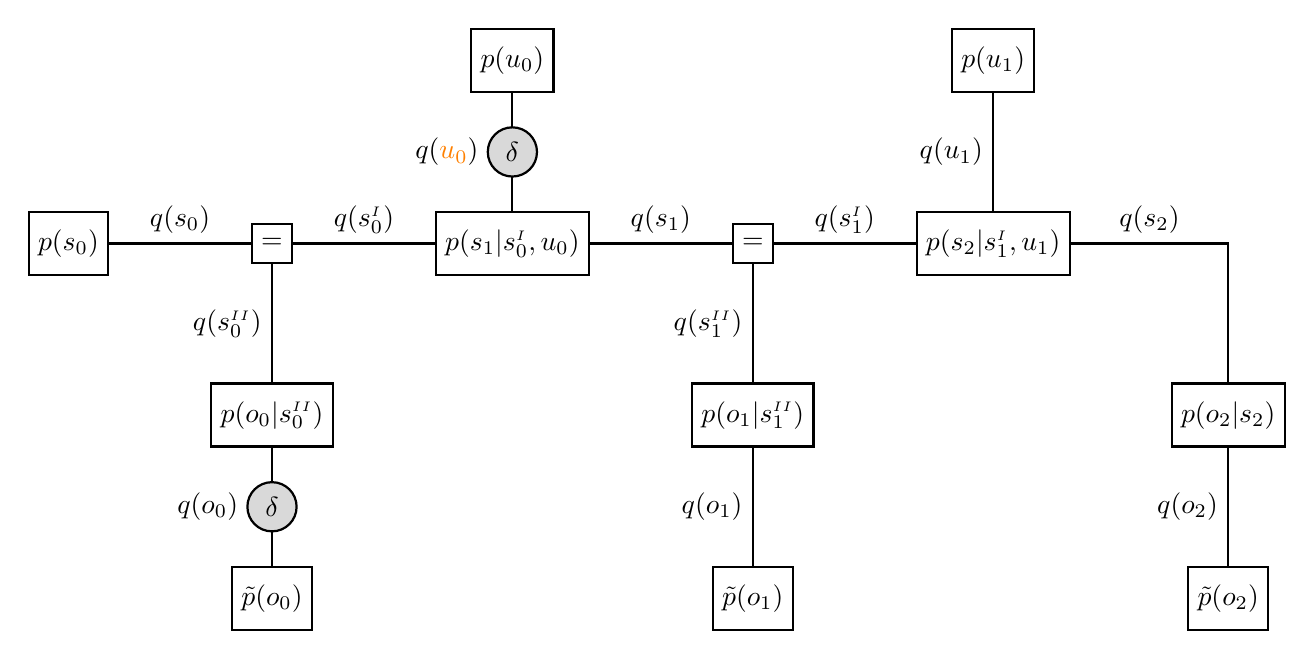
\begin{tikzpicture}[
    factor/.style={draw=black, thick, rectangle, minimum size=0.8cm, font=\normalsize},
    eqfactor/.style={draw=black, thick, rectangle, minimum size=0.5cm, font=\normalsize},
    edge/.style={thick},
    varlabel/.style={font=\normalsize},
    greycircle/.style={draw=black, thick, circle, fill=gray!30, minimum size=0.5cm, font=\normalsize}
]

% Knoten
\node[factor] (d) {$p(s_0)$};
\node[eqfactor, right=1.8cm of d] (eq0) {$=$};
\node[factor, below=1.5cm of eq0] (A0) {$p(o_0|s^{\scriptscriptstyle II}_0)$};
\node[factor, below=1.5cm of A0] (c0) {$\tilde{p}(o_0)$};
\node[factor, right=1.8cm of eq0] (B0) {$p(s_1|s^{\scriptscriptstyle I}_0,u_0)$};
\node[eqfactor, right=1.8cm of B0] (eq1) {$=$};
\node[factor, below=1.5cm of eq1] (A1) {$p(o_1|s^{\scriptscriptstyle II}_1)$};
\node[factor, below=1.5cm of A1] (c1) {$\tilde{p}(o_1)$};
\node[factor, right=1.8cm of eq1] (B1) {$p(s_2|s^{\scriptscriptstyle I}_1,u_1)$};
\node[factor] (A2) at ([xshift=2cm] B1.east |- A1) {$p(o_2|s_2)$};
\node[factor, below=1.5cm of A2] (c2) {$\tilde{p}(o_2)$};
\node[factor, above=1.5cm of B0] (u0) {$p(u_0)$};
\node[factor, above=1.5cm of B1] (u1) {$p(u_1)$};

% Kanten zwischen Knoten
\draw[edge] (d.east) -- (eq0.west) node[midway, above, varlabel] {$\textcolor{black}{q(s_0)}$};
\draw[edge] (eq0.south) -- (A0.north) node[midway, left, varlabel] {$\textcolor{black}{q(s^{\scriptscriptstyle II}_0)}$};
\draw[edge] (A0.south) -- (c0.north) node[midway, greycircle] {$\delta$} node[midway, left=0.3, varlabel] {$q(\textcolor{black}{o_0})$};
\draw[edge] (eq0.east) -- (B0.west) node[midway, above, varlabel] {$\textcolor{black}{q(s^{\scriptscriptstyle I}_0)}$};
\draw[edge] (B0.north) -- (u0.south) node[midway, greycircle] {$\delta$} node[midway, left=0.3, varlabel] {$q(\textcolor{orange}{u_0})$};
\draw[edge] (B0.east) -- (eq1.west) node[midway, above, varlabel] {$\textcolor{black}{q(s_1)}$};
\draw[edge] (eq1.south) -- (A1.north) node[midway, left, varlabel] {$\textcolor{black}{q(s^{\scriptscriptstyle II}_1)}$};
\draw[edge] (A1.south) -- (c1.north) node[midway, left, varlabel] {$\textcolor{black}{q(o_1)}$};
\draw[edge] (eq1.east) -- (B1.west) node[midway, above, varlabel] {$\textcolor{black}{q(s^{\scriptscriptstyle I}_1)}$};
\draw[edge] (B1.east) -| (A2.north) node[pos=0.25, above, varlabel] {$\textcolor{black}{q(s_2)}$};
\draw[edge] (A2.south) -- (c2.north) node[midway, left, varlabel] {$\textcolor{black}{q(o_2)}$};
\draw[edge] (B1.north) -- (u1.south) node[midway, left, varlabel] {$\textcolor{black}{q(u_1)}$};

\end{tikzpicture}}
                \end{tabular}%
                \llap{\smash{\raisebox{2.0cm}[0pt][0pt]{\sffamily\bfseries\small (b)\hspace*{-0.0cm}}}}%
                \hspace{0.1cm}% 3. Fester Abstand: RECHTS VOM FFG (Zum Box-Rand)
                \vspace{0.02cm} % 4. Fester Abstand: UNTEN
            \end{minipage}%
        }
        \phantomcaption
        \label{fig:25.2}
    \end{subfigure}

    \vspace{0.2cm} % Abstand zwischen den Kästen

    % ================= TIMESTEP 1 =================
    \begin{subfigure}[b]{\textwidth}
        \centering
        \fbox{%
            \begin{minipage}{0.97\linewidth}
                \vspace{0.15cm} % 1. Fester Abstand: OBEN
                % ==========================================
                % BEREICH 1: Das T-Maze (Flexibel zentriert)
                % ==========================================
                \hfill % Drückt das Maze von links weg
                \begin{tabular}{@{}c@{}}
                    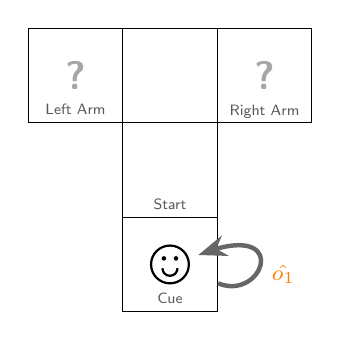
\begin{tikzpicture}[scale=1.2]
                        \tikzset{
                            agent/.pic={
                                    \node[circle, draw=black, thick, fill=white, minimum size=0.5cm] at (0,0) {};
                                    \fill[black] (-0.08, 0.08) circle (0.03);
                                    \fill[black] (0.08, 0.08) circle (0.03);
                                    \draw[thick] (-0.1, -0.05) arc (180:360:0.1);
                                },
                            field label/.style={
                                    font=\tiny\sffamily, text=gray!70!black, anchor=south, scale=0.9, transform shape
                                },
                            field symbol/.style={
                                    font=\large\bfseries,
                                    text=gray!70,
                                    anchor=center,
                                    scale=1.0,
                                    transform shape
                                }
                        }

                        \draw (-0.5, 0) -- (-0.5, 2.0) -- (-1.5, 2.0) -- (-1.5, 3.0) -- (1.5, 3.0) -- (1.5, 2.0) -- (0.5, 2.0) -- (0.5, 0) -- cycle;
                        \draw (-0.5, 1.0) -- (0.5, 1.0);
                        \draw (-0.5, 2.0) -- (0.5, 2.0);
                        \draw (-0.5, 2.0) -- (-0.5, 3.0);
                        \draw (0.5, 2.0) -- (0.5, 3.0);

                        \pic[scale=0.8, transform shape] at (0, 0.5) {agent};
                        % Observation Arrow
                        \draw[
                            -{Stealth[scale=1.0]},
                            line width=1.6pt,
                            color=gray!80!black
                        ]
                        (0.51, 0.3) .. controls (1.0, 0.1) and (1.3, 1.0) .. (0.3, 0.6);
                        \node[font=\footnotesize, text=gray!80!black] at (1.2, 0.4) {$\textcolor{orange}{\hat {o_1}}$};
                        \node[field label] at (0, 0.97) {Start};
                        \node[field label] at (0, -0.03) {Cue};
                        \node[field label] at (-1.0, 1.97) {Left Arm};
                        \node[field label] at (1.0, 1.93) {Right Arm};
                        %\node[field symbol] at (0, 0.5) {!};
                        \node[field symbol] at (-1.0, 2.5) {?};
                        \node[field symbol] at (1.0, 2.5) {?};
                    \end{tikzpicture}
                \end{tabular}%
                \hfill % Drückt das Maze von der gestrichelten Linie weg (zentriert es somit perfekt im linken Rest-Raum)
                % ==========================================
                % BEREICH 2: Die Trennlinie
                % ==========================================
                \begin{tabular}{@{}c@{}}
                    \tikz \draw[dashed, thin, gray] (0,-2.1) -- (0,2.1);
                \end{tabular}%
                \hspace{0.3cm}% 2. Fester Abstand: LINKS VOM FFG
                % ==========================================
                % BEREICH 3: Der FFG (gibt die Breite vor)
                % ==========================================
                \begin{tabular}{@{}c@{}}
                    % Der FFG wird jetzt in seiner absolut natürlichen Größe gerendert.
                    \resizebox{9cm}{!}{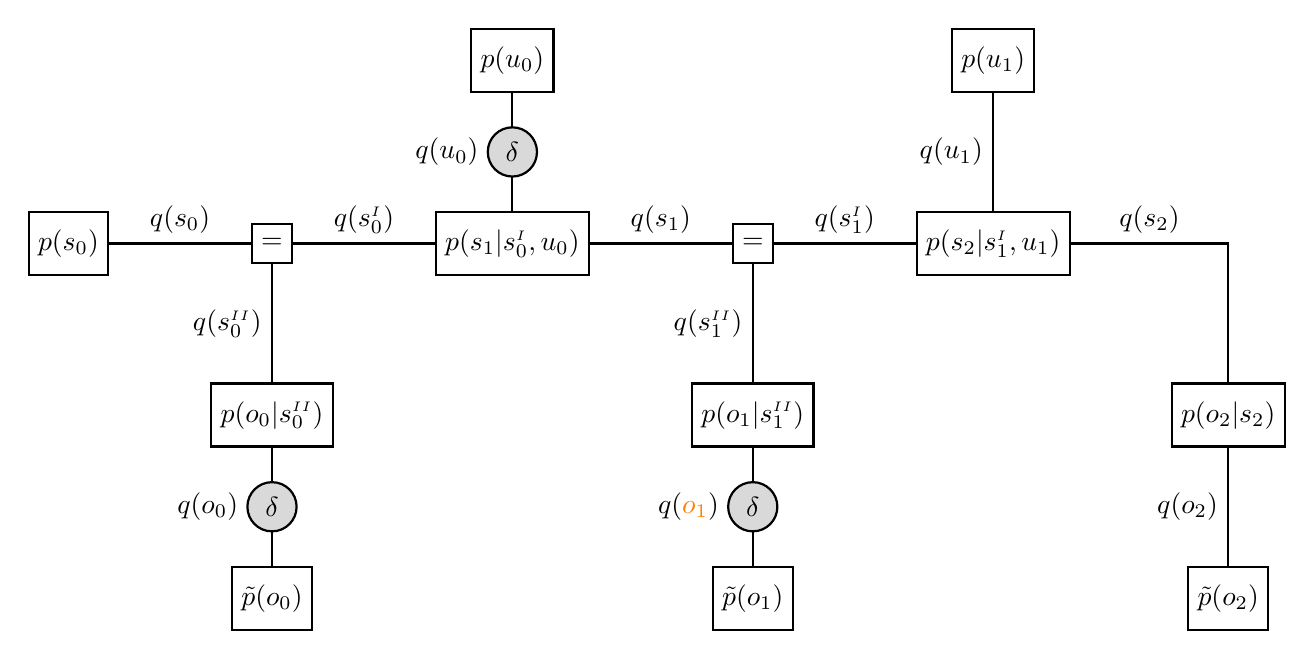
\begin{tikzpicture}[
    factor/.style={draw=black, thick, rectangle, minimum size=0.8cm, font=\normalsize},
    eqfactor/.style={draw=black, thick, rectangle, minimum size=0.5cm, font=\normalsize},
    edge/.style={thick},
    varlabel/.style={font=\normalsize},
    greycircle/.style={draw=black, thick, circle, fill=gray!30, minimum size=0.5cm, font=\normalsize}
]

% Knoten
\node[factor] (d) {$p(s_0)$};
\node[eqfactor, right=1.8cm of d] (eq0) {$=$};
\node[factor, below=1.5cm of eq0] (A0) {$p(o_0|s^{\scriptscriptstyle II}_0)$};
\node[factor, below=1.5cm of A0] (c0) {$\tilde{p}(o_0)$};
\node[factor, right=1.8cm of eq0] (B0) {$p(s_1|s^{\scriptscriptstyle I}_0,u_0)$};
\node[eqfactor, right=1.8cm of B0] (eq1) {$=$};
\node[factor, below=1.5cm of eq1] (A1) {$p(o_1|s^{\scriptscriptstyle II}_1)$};
\node[factor, below=1.5cm of A1] (c1) {$\tilde{p}(o_1)$};
\node[factor, right=1.8cm of eq1] (B1) {$p(s_2|s^{\scriptscriptstyle I}_1,u_1)$};
\node[factor] (A2) at ([xshift=2cm] B1.east |- A1) {$p(o_2|s_2)$};
\node[factor, below=1.5cm of A2] (c2) {$\tilde{p}(o_2)$};
\node[factor, above=1.5cm of B0] (u0) {$p(u_0)$};
\node[factor, above=1.5cm of B1] (u1) {$p(u_1)$};

% Kanten zwischen Knoten
\draw[edge] (d.east) -- (eq0.west) node[midway, above, varlabel] {$\textcolor{black}{q(s_0)}$};
\draw[edge] (eq0.south) -- (A0.north) node[midway, left, varlabel] {$\textcolor{black}{q(s^{\scriptscriptstyle II}_0)}$};
\draw[edge] (A0.south) -- (c0.north) node[midway, greycircle] {$\delta$} node[midway, left=0.3, varlabel] {$q(\textcolor{black}{o_0})$};
\draw[edge] (eq0.east) -- (B0.west) node[midway, above, varlabel] {$\textcolor{black}{q(s^{\scriptscriptstyle I}_0)}$};
\draw[edge] (B0.north) -- (u0.south) node[midway, greycircle] {$\delta$} node[midway, left=0.3, varlabel] {$q(\textcolor{black}{u_0})$};
\draw[edge] (B0.east) -- (eq1.west) node[midway, above, varlabel] {$\textcolor{black}{q(s_1)}$};
\draw[edge] (eq1.south) -- (A1.north) node[midway, left, varlabel] {$\textcolor{black}{q(s^{\scriptscriptstyle II}_1)}$};
\draw[edge] (A1.south) -- (c1.north) node[midway, greycircle] {$\delta$} node[midway, left=0.3, varlabel] {$q(\textcolor{orange}{o_1})$};
\draw[edge] (eq1.east) -- (B1.west) node[midway, above, varlabel] {$\textcolor{black}{q(s^{\scriptscriptstyle I}_1)}$};
\draw[edge] (B1.east) -| (A2.north) node[pos=0.25, above, varlabel] {$\textcolor{black}{q(s_2)}$};
\draw[edge] (A2.south) -- (c2.north) node[midway, left, varlabel] {$\textcolor{black}{q(o_2)}$};
\draw[edge] (B1.north) -- (u1.south) node[midway, left, varlabel] {$\textcolor{black}{q(u_1)}$};

\end{tikzpicture}}
                \end{tabular}%
                \llap{\smash{\raisebox{2.0cm}[0pt][0pt]{\sffamily\bfseries\small (c)\hspace*{-0.0cm}}}}%
                \hspace{0.1cm}% 3. Fester Abstand: RECHTS VOM FFG (Zum Box-Rand)
                \vspace{0.02cm} % 4. Fester Abstand: UNTEN
            \end{minipage}%
        }
        \phantomcaption
        \label{fig:25.3}
    \end{subfigure}
    %\vspace{0.2cm} % Abstand zwischen den Kästen
\end{figure}

\begin{figure}[htbp]
    \ContinuedFloat

    % ================= TIMESTEP 1 =================
    \begin{subfigure}[b]{\textwidth}
        \centering
        \fbox{%
            \begin{minipage}{0.97\linewidth}
                \vspace{0.15cm} % 1. Fester Abstand: OBEN
                % ==========================================
                % BEREICH 1: Das T-Maze (Flexibel zentriert)
                % ==========================================
                \hfill % Drückt das Maze von links weg
                \begin{tabular}{@{}c@{}}
                    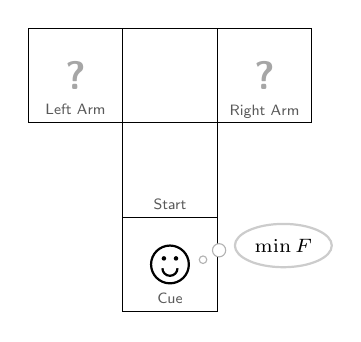
\begin{tikzpicture}[scale=1.2]
                        \tikzset{
                            agent/.pic={
                                    \node[circle, draw=black, thick, fill=white, minimum size=0.5cm] at (0,0) {};
                                    \fill[black] (-0.08, 0.08) circle (0.03);
                                    \fill[black] (0.08, 0.08) circle (0.03);
                                    \draw[thick] (-0.1, -0.05) arc (180:360:0.1);
                                },
                            field label/.style={
                                    font=\tiny\sffamily, text=gray!70!black, anchor=south, scale=0.9, transform shape
                                },
                            field symbol/.style={
                                    font=\large\bfseries,
                                    text=gray!70,
                                    anchor=center,
                                    scale=1.0,
                                    transform shape
                                }
                        }

                        \draw (-0.5, 0) -- (-0.5, 2.0) -- (-1.5, 2.0) -- (-1.5, 3.0) -- (1.5, 3.0) -- (1.5, 2.0) -- (0.5, 2.0) -- (0.5, 0) -- cycle;
                        \draw (-0.5, 1.0) -- (0.5, 1.0);
                        \draw (-0.5, 2.0) -- (0.5, 2.0);
                        \draw (-0.5, 2.0) -- (-0.5, 3.0);
                        \draw (0.5, 2.0) -- (0.5, 3.0);

                        \pic[scale=0.8, transform shape] at (0, 0.5) {agent};
                        \node[field label] at (0, 0.97) {Start};
                        \node[field label] at (0, -0.03) {Cue};
                        \node[field label] at (-1.0, 1.97) {Left Arm};
                        \node[field label] at (1.0, 1.93) {Right Arm};
                        %\node[field symbol] at (0, 0.5) {!};
                        \node[field symbol] at (-1.0, 2.5) {?};
                        \node[field symbol] at (1.0, 2.5) {?};

                        % --- NEU: Gedankenblase für Variational Free Energy Minimierung ---
                        % Kleine Bläschen, die vom Kopf (ca. 0.3, 1.7) nach rechts oben steigen
                        \draw[thin, gray!60, fill=white] (0.35, 0.55) circle (0.04);
                        \draw[thin, gray!60, fill=white] (0.52, 0.65) circle (0.07);

                        % Die Haupt-Gedankenblase mit dem Minimierungs-Symbol / Free Energy F
                        \node[
                            ellipse,
                            draw=gray!40,
                            thick,
                            fill=white,
                            minimum width=1.0cm,
                            minimum height=0.55cm,
                            inner sep=2pt,
                            font=\scriptsize\sffamily,
                            text=black!100!black
                        ] at (1.2, 0.7) {$\min F$};
                    \end{tikzpicture}
                \end{tabular}%
                \hfill % Drückt das Maze von der gestrichelten Linie weg (zentriert es somit perfekt im linken Rest-Raum)
                % ==========================================
                % BEREICH 2: Die Trennlinie
                % ==========================================
                \begin{tabular}{@{}c@{}}
                    \tikz \draw[dashed, thin, gray] (0,-2.1) -- (0,2.1);
                \end{tabular}%
                \hspace{0.3cm}% 2. Fester Abstand: LINKS VOM FFG
                % ==========================================
                % BEREICH 3: Der FFG (gibt die Breite vor)
                % ==========================================
                \begin{tabular}{@{}c@{}}
                    % Der FFG wird jetzt in seiner absolut natürlichen Größe gerendert.
                    \resizebox{9cm}{!}{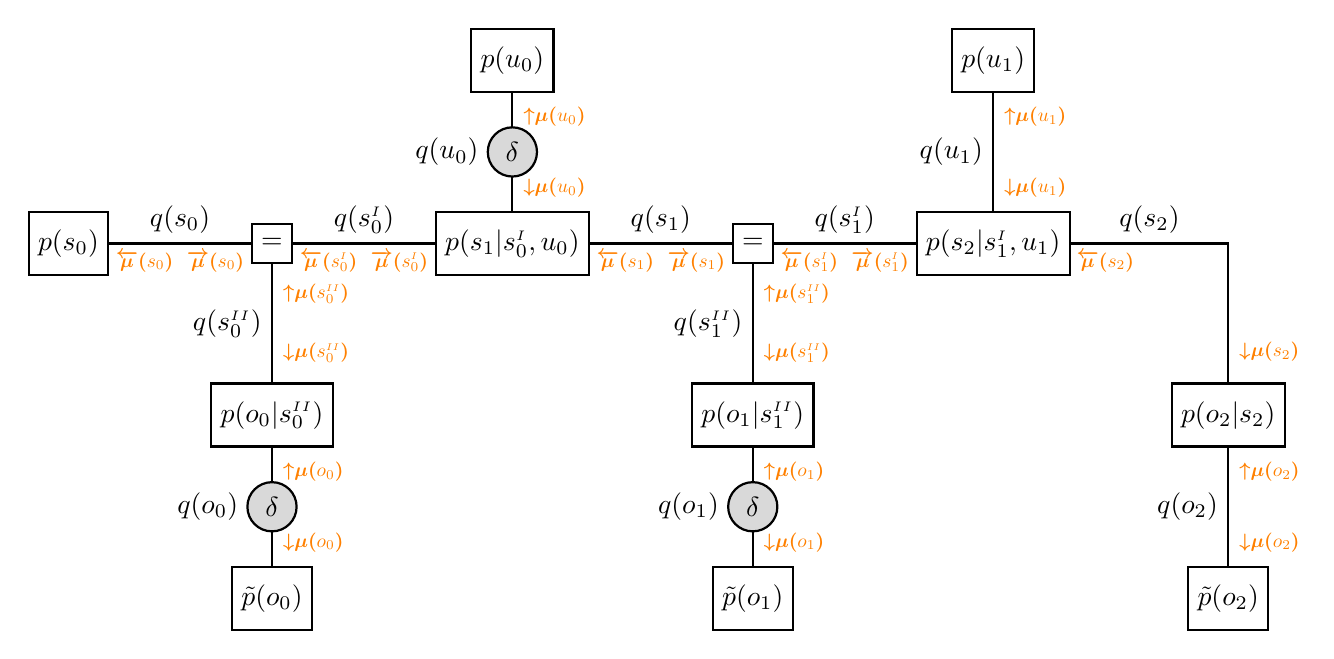
\begin{tikzpicture}[
    factor/.style={draw=black, thick, rectangle, minimum size=0.8cm, font=\normalsize},
    eqfactor/.style={draw=black, thick, rectangle, minimum size=0.5cm, font=\normalsize},
    edge/.style={thick},
    varlabel/.style={font=\normalsize},
    greycircle/.style={draw=black, thick, circle, fill=gray!30, minimum size=0.5cm, font=\normalsize}
]

% Knoten
\node[factor] (d) {$p(s_0)$};
\node[eqfactor, right=1.8cm of d] (eq0) {$=$};
\node[factor, below=1.5cm of eq0] (A0) {$p(o_0|s^{\scriptscriptstyle II}_0)$};
\node[factor, below=1.5cm of A0] (c0) {$\tilde{p}(o_0)$};
\node[factor, right=1.8cm of eq0] (B0) {$p(s_1|s^{\scriptscriptstyle I}_0,u_0)$};
\node[eqfactor, right=1.8cm of B0] (eq1) {$=$};
\node[factor, below=1.5cm of eq1] (A1) {$p(o_1|s^{\scriptscriptstyle II}_1)$};
\node[factor, below=1.5cm of A1] (c1) {$\tilde{p}(o_1)$};
\node[factor, right=1.8cm of eq1] (B1) {$p(s_2|s^{\scriptscriptstyle I}_1,u_1)$};
\node[factor] (A2) at ([xshift=2cm] B1.east |- A1) {$p(o_2|s_2)$};
\node[factor, below=1.5cm of A2] (c2) {$\tilde{p}(o_2)$};
\node[factor, above=1.5cm of B0] (u0) {$p(u_0)$};
\node[factor, above=1.5cm of B1] (u1) {$p(u_1)$};

% Kanten zwischen Knoten
\draw[edge] (d.east) -- (eq0.west) node[midway, above, varlabel] {$\textcolor{black}{q(s_0)}$} node[near end, below, varlabel, scale=0.7] {$\textcolor{orange}{\bm{\overrightarrow{\mu}(}s_0\bm{)}}$} node[near start, below, varlabel, scale=0.7] {$\textcolor{orange}{\bm{\overleftarrow{\mu}(}s_0\bm{)}}$};
\draw[edge] (eq0.south) -- (A0.north) node[midway, left, varlabel] {$\textcolor{black}{q(s^{\scriptscriptstyle II}_0)}$} node[pos=0.25, right=0.05, varlabel, scale=0.7] {$\textcolor{orange}{\bm{{\uparrow}{\mu}(}s^{\scriptscriptstyle II}_0\bm{)}}$} node[pos=0.75, right=0.05, varlabel, scale=0.7] {$\textcolor{orange}{\bm{{\downarrow}{\mu}(}s^{\scriptscriptstyle II}_0\bm{)}}$};
\draw[edge] (A0.south) -- (c0.north) node[midway, greycircle] {$\delta$} node[midway, left=0.3, varlabel] {$\textcolor{black}{q(o_0)}$} node[pos=0.2, right=0.05, varlabel, scale=0.7] {$\textcolor{orange}{\bm{{\uparrow}{\mu}(}o_0\bm{)}}$} node[pos=0.8, right=0.05, varlabel, scale=0.7] {$\textcolor{orange}{\bm{{\downarrow}{\mu}(}o_0\bm{)}}$};
\draw[edge] (eq0.east) -- (B0.west) node[midway, above, varlabel] {$\textcolor{black}{q(s^{\scriptscriptstyle I}_0)}$} node[near start, below, varlabel, scale=0.7] {$\textcolor{orange}{\bm{\overleftarrow{\mu}(}s^{\scriptscriptstyle I}_0\bm{)}}$} node[near end, below, varlabel, scale=0.7] {$\textcolor{orange}{\bm{\overrightarrow{\mu}(}s^{\scriptscriptstyle I}_0\bm{)}}$};
\draw[edge] (B0.north) -- (u0.south) node[midway, greycircle] {$\delta$} node[midway, left=0.3, varlabel] {$\textcolor{black}{q(u_0)}$} node[pos=0.2, right=0.05, varlabel, scale=0.7] {$\textcolor{orange}{\bm{{\downarrow}{\mu}(}u_0\bm{)}}$} node[pos=0.8, right=0.05, varlabel, scale=0.7] {$\textcolor{orange}{\bm{{\uparrow}{\mu}(}u_0\bm{)}}$};
\draw[edge] (B0.east) -- (eq1.west) node[midway, above, varlabel] {$\textcolor{black}{q(s_1)}$} node[near end, below, varlabel, scale=0.7] {$\textcolor{orange}{\bm{\overrightarrow{\mu}(}s_1\bm{)}}$} node[near start, below, varlabel, scale=0.7] {$\textcolor{orange}{\bm{\overleftarrow{\mu}(}s_1\bm{)}}$};
\draw[edge] (eq1.south) -- (A1.north) node[midway, left, varlabel] {$\textcolor{black}{q(s^{\scriptscriptstyle II}_1)}$} node[pos=0.25, right=0.05, varlabel, scale=0.7] {$\textcolor{orange}{\bm{{\uparrow}{\mu}(}s^{\scriptscriptstyle II}_1\bm{)}}$} node[pos=0.75, right=0.05, varlabel, scale=0.7] {$\textcolor{orange}{\bm{{\downarrow}{\mu}(}s^{\scriptscriptstyle II}_1\bm{)}}$};
\draw[edge] (A1.south) -- (c1.north) node[midway, greycircle] {$\delta$} node[midway, left=0.3, varlabel] {$\textcolor{black}{q(o_1)}$} node[pos=0.2, right=0.05, varlabel, scale=0.7] {$\textcolor{orange}{\bm{{\uparrow}{\mu}(}o_1\bm{)}}$} node[pos=0.8, right=0.05, varlabel, scale=0.7] {$\textcolor{orange}{\bm{{\downarrow}{\mu}(}o_1\bm{)}}$};
\draw[edge] (eq1.east) -- (B1.west) node[midway, above, varlabel] {$\textcolor{black}{q(s^{\scriptscriptstyle I}_1)}$} node[near start, below, varlabel, scale=0.7] {$\textcolor{orange}{\bm{\overleftarrow{\mu}(}s^{\scriptscriptstyle I}_1\bm{)}}$} node[near end, below, varlabel, scale=0.7] {$\textcolor{orange}{\bm{\overrightarrow{\mu}(}s^{\scriptscriptstyle I}_1\bm{)}}$};
\draw[edge] (B1.east) -| (A2.north) node[pos=0.25, above, varlabel] {$\textcolor{black}{q(s_2)}$} node[pos=0.89, right=0.05, varlabel, scale=0.7] {$\textcolor{orange}{\bm{{\downarrow}{\mu}(}s_2\bm{)}}$} node[pos=0.11, below, varlabel, scale=0.7] {$\textcolor{orange}{\bm{\overleftarrow{\mu}(}s_2\bm{)}}$};
\draw[edge] (A2.south) -- (c2.north) node[midway, left, varlabel] {$\textcolor{black}{q(o_2)}$} node[pos=0.2, right=0.05, varlabel, scale=0.7] {$\textcolor{orange}{\bm{{\uparrow}{\mu}(}o_2\bm{)}}$} node[pos=0.8, right=0.05, varlabel, scale=0.7] {$\textcolor{orange}{\bm{{\downarrow}{\mu}(}o_2\bm{)}}$};
\draw[edge] (B1.north) -- (u1.south) node[midway, left, varlabel] {$\textcolor{black}{q(u_1)}$} node[pos=0.2, right=0.05, varlabel, scale=0.7] {$\textcolor{orange}{\bm{{\downarrow}{\mu}(}u_1\bm{)}}$} node[pos=0.8, right=0.05, varlabel, scale=0.7] {$\textcolor{orange}{\bm{{\uparrow}{\mu}(}u_1\bm{)}}$};

\end{tikzpicture}}
                \end{tabular}%
                \llap{\smash{\raisebox{2.0cm}[0pt][0pt]{\sffamily\bfseries\small (d)\hspace*{-0.0cm}}}}%
                \hspace{0.1cm}% 3. Fester Abstand: RECHTS VOM FFG (Zum Box-Rand)
                \vspace{0.02cm} % 4. Fester Abstand: UNTEN
            \end{minipage}%
        }
        \phantomcaption
        \label{fig:25.4}
    \end{subfigure}

    \caption{The figure presents the four steps of the simulation "Exploiting Information" via the example of the BFE agent. First, the agents receives an observation \(\hat {o_0}\) which makes \(q(o_0\) a delta distribution with all its probability mass at \(\hat {o_0}\) (\cref{fig:25.1}). Second, the action "go to cue" is externally triggered and the respective belief distribution \(q(u_0)\) also becomes a delta distribution with its mass at this action (\cref{fig:25.2}). Third, being at the cue triggeres an observation from the environment that is informative regarding the reward location. Similar to the first observation, it leads to a delta distribution at \(q(o_1)\) (\cref{fig:25.3}). Lastly, the agent executes its message passing algorithm to infer all its belief distributions (\cref{fig:25.4}). The inclination of moving to the cued arm that promises the reward is then given as a probability in the action-specific belief distribution \(q(u_1)\).}
    \label{fig:25}
\end{figure}

\subsubsection{Experiment 3: Long-Term Success}

This experiment is about empirically measuring the agents' succes in receiving the reward during a trial. Specifically, there are two ways how an agent can achieve this: First, it initially "decides" against going to the cue and instead moves to one of the two arms. It is then either lucky and observes the reward or not. Second, the agent initially moves to the cue and only then moves to one of the two arms. Again, it then either observes the reward or not. Generally, a trial consists of three timesteps \(t \in {0,1,2}\) and the agent can either observe the reward in timestep \(t=1\) (when directly moving to an arm) or in timestep \(t=2\) (when first moving to the cue in \(t=1\)). A trial is succesfull when the agent observes the reward in timesteps \(t=1\) or \(t=2\) (a trial is prematurely terminated when it receives in reward in timestep \(t=1\)). There are \(1000\) trials for each agent (and \(\alpha\)- and \(c\) value). The result is the percentage of succesfull trials. The procedere is detailed in \cref{fig:26}.

\begin{figure}[b!]
    \centering

    % ================= TIMESTEP 1.1 =================
    \begin{subfigure}[b]{0.49\textwidth}
        \centering
        \fbox{%
            \begin{minipage}{0.97\linewidth}
                \vspace{0.15cm} % 1. Fester Abstand: OBEN
                % ==========================================
                % BEREICH 1: Das T-Maze (Flexibel zentriert)
                % ==========================================
                \hfill % Drückt das Maze von links weg
                \begin{tabular}{@{}c@{}}
                    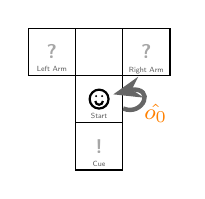
\begin{tikzpicture}[scale=0.6]
                        \tikzset{
                            agent/.pic={
                                    \node[circle, draw=black, thick, fill=white, minimum size=0.5cm] at (0,0) {};
                                    \fill[black] (-0.08, 0.08) circle (0.03);
                                    \fill[black] (0.08, 0.08) circle (0.03);
                                    \draw[thick] (-0.1, -0.05) arc (180:360:0.1);
                                },
                            field label/.style={
                                    font=\tiny\sffamily, text=gray!70!black, anchor=south, scale=0.9, transform shape
                                },
                            field symbol/.style={
                                    font=\large\bfseries,
                                    text=gray!70,
                                    anchor=center,
                                    scale=1.0,
                                    transform shape
                                }
                        }

                        \draw (-0.5, 0) -- (-0.5, 2.0) -- (-1.5, 2.0) -- (-1.5, 3.0) -- (1.5, 3.0) -- (1.5, 2.0) -- (0.5, 2.0) -- (0.5, 0) -- cycle;
                        \draw (-0.5, 1.0) -- (0.5, 1.0);
                        \draw (-0.5, 2.0) -- (0.5, 2.0);
                        \draw (-0.5, 2.0) -- (-0.5, 3.0);
                        \draw (0.5, 2.0) -- (0.5, 3.0);

                        \pic[scale=0.8, transform shape] at (0, 1.5) {agent};
                        % Observation Arrow
                        \draw[
                            -{Stealth[scale=1.0]},
                            line width=1.6pt,
                            color=gray!80!black
                        ]
                        (0.51, 1.3) .. controls (1.0, 1.1) and (1.3, 2.0) .. (0.3, 1.6);
                        \node[font=\footnotesize, text=gray!80!black] at (1.2, 1.2) {$\textcolor{orange}{\hat {o_0}}$};
                        \node[field label] at (0, 0.97) {Start};
                        \node[field label] at (0, -0.03) {Cue};
                        \node[field label] at (-1.0, 1.97) {Left Arm};
                        \node[field label] at (1.0, 1.93) {Right Arm};
                        \node[field symbol] at (0, 0.5) {!};
                        \node[field symbol] at (-1.0, 2.5) {?};
                        \node[field symbol] at (1.0, 2.5) {?};
                    \end{tikzpicture}
                \end{tabular}%
                \hfill % Drückt das Maze von der gestrichelten Linie weg (zentriert es somit perfekt im linken Rest-Raum)
                % ==========================================
                % BEREICH 2: Die Trennlinie
                % ==========================================
                \begin{tabular}{@{}c@{}}
                    \tikz \draw[dashed, thin, gray] (0,-1.05) -- (0,1.05);
                \end{tabular}%
                \hspace{0.3cm}% 2. Fester Abstand: LINKS VOM FFG
                % ==========================================
                % BEREICH 3: Der FFG (gibt die Breite vor)
                % ==========================================
                \begin{tabular}{@{}c@{}}
                    % Der FFG wird jetzt in seiner absolut natürlichen Größe gerendert.
                    \resizebox{4.5cm}{!}{\begin{tikzpicture}[
    factor/.style={draw=black, thick, rectangle, minimum size=0.8cm, font=\normalsize},
    eqfactor/.style={draw=black, thick, rectangle, minimum size=0.5cm, font=\normalsize},
    edge/.style={thick},
    varlabel/.style={font=\normalsize},
    greycircle/.style={draw=black, thick, circle, fill=gray!30, minimum size=0.5cm, font=\normalsize}
]

% Knoten
\node[factor] (d) {$p(s_0)$};
\node[eqfactor, right=1.8cm of d] (eq0) {$=$};
\node[factor, below=1.5cm of eq0] (A0) {$p(o_0|s^{\scriptscriptstyle II}_0)$};
\node[factor, below=1.5cm of A0] (c0) {$\tilde{p}(o_0)$};
\node[factor, right=1.8cm of eq0] (B0) {$p(s_1|s^{\scriptscriptstyle I}_0,u_0)$};
\node[eqfactor, right=1.8cm of B0] (eq1) {$=$};
\node[factor, below=1.5cm of eq1] (A1) {$p(o_1|s^{\scriptscriptstyle II}_1)$};
\node[factor, below=1.5cm of A1] (c1) {$\tilde{p}(o_1)$};
\node[factor, right=1.8cm of eq1] (B1) {$p(s_2|s^{\scriptscriptstyle I}_1,u_1)$};
\node[factor] (A2) at ([xshift=2cm] B1.east |- A1) {$p(o_2|s_2)$};
\node[factor, below=1.5cm of A2] (c2) {$\tilde{p}(o_2)$};
\node[factor, above=1.5cm of B0] (u0) {$p(u_0)$};
\node[factor, above=1.5cm of B1] (u1) {$p(u_1)$};

% Kanten zwischen Knoten
\draw[edge] (d.east) -- (eq0.west) node[midway, above, varlabel] {$\textcolor{black}{q(s_0)}$};
\draw[edge] (eq0.south) -- (A0.north) node[midway, left, varlabel] {$\textcolor{black}{q(s^{\scriptscriptstyle II}_0)}$};
\draw[edge] (A0.south) -- (c0.north) node[midway, greycircle] {$\delta$} node[midway, left=0.3, varlabel] {$q(\textcolor{orange}{o_0})$};
\draw[edge] (eq0.east) -- (B0.west) node[midway, above, varlabel] {$\textcolor{black}{q(s^{\scriptscriptstyle I}_0)}$};
\draw[edge] (B0.north) -- (u0.south) node[midway, left, varlabel] {$\textcolor{black}{q(u_0)}$};
\draw[edge] (B0.east) -- (eq1.west) node[midway, above, varlabel] {$\textcolor{black}{q(s_1)}$};
\draw[edge] (eq1.south) -- (A1.north) node[midway, left, varlabel] {$\textcolor{black}{q(s^{\scriptscriptstyle II}_1)}$};
\draw[edge] (A1.south) -- (c1.north) node[midway, left, varlabel] {$\textcolor{black}{q(o_1)}$};
\draw[edge] (eq1.east) -- (B1.west) node[midway, above, varlabel] {$\textcolor{black}{q(s^{\scriptscriptstyle I}_1)}$};
\draw[edge] (B1.east) -| (A2.north) node[pos=0.25, above, varlabel] {$\textcolor{black}{q(s_2)}$};
\draw[edge] (A2.south) -- (c2.north) node[midway, left, varlabel] {$\textcolor{black}{q(o_2)}$};
\draw[edge] (B1.north) -- (u1.south) node[midway, left, varlabel] {$\textcolor{black}{q(u_1)}$};

\end{tikzpicture}}
                \end{tabular}%
                \llap{\smash{\raisebox{1.0cm}[0pt][0pt]{\sffamily\bfseries\small (a)\hspace*{-0.05cm}}}}%
                \hspace{0.1cm}% 3. Fester Abstand: RECHTS VOM FFG (Zum Box-Rand)
                \vspace{0.02cm} % 4. Fester Abstand: UNTEN
            \end{minipage}%
        }
        \phantomcaption
        \label{fig:26.1a}
    \end{subfigure}
    \hfill
    % ================= TIMESTEP 1.2 =================
    \begin{subfigure}[b]{0.49\textwidth}
        \centering
        \fbox{%
            \begin{minipage}{0.97\linewidth}
                \vspace{0.15cm} % 1. Fester Abstand: OBEN
                % ==========================================
                % BEREICH 1: Das T-Maze (Flexibel zentriert)
                % ==========================================
                \hfill % Drückt das Maze von links weg
                \begin{tabular}{@{}c@{}}
                    \begin{tikzpicture}[scale=0.6]
                        \tikzset{
                            agent/.pic={
                                    \node[circle, draw=black, thick, fill=white, minimum size=0.5cm] at (0,0) {};
                                    \fill[black] (-0.08, 0.08) circle (0.03);
                                    \fill[black] (0.08, 0.08) circle (0.03);
                                    \draw[thick] (-0.1, -0.05) arc (180:360:0.1);
                                },
                            field label/.style={
                                    font=\tiny\sffamily, text=gray!70!black, anchor=south, scale=0.9, transform shape
                                },
                            field symbol/.style={
                                    font=\large\bfseries,
                                    text=gray!70,
                                    anchor=center,
                                    scale=1.0,
                                    transform shape
                                }
                        }

                        \draw (-0.5, 0) -- (-0.5, 2.0) -- (-1.5, 2.0) -- (-1.5, 3.0) -- (1.5, 3.0) -- (1.5, 2.0) -- (0.5, 2.0) -- (0.5, 0) -- cycle;
                        \draw (-0.5, 1.0) -- (0.5, 1.0);
                        \draw (-0.5, 2.0) -- (0.5, 2.0);
                        \draw (-0.5, 2.0) -- (-0.5, 3.0);
                        \draw (0.5, 2.0) -- (0.5, 3.0);

                        \pic[scale=0.8, transform shape] at (0, 1.5) {agent};
                        % Observation Arrow
                        \draw[
                            -{Stealth[scale=1.0]},
                            line width=1.6pt,
                            color=gray!80!black
                        ]
                        (0.51, 1.3) .. controls (1.0, 1.1) and (1.3, 2.0) .. (0.3, 1.6);
                        \node[font=\footnotesize, text=gray!80!black] at (1.2, 1.2) {$\textcolor{orange}{\hat {o_0}}$};
                        \node[field label] at (0, 0.97) {Start};
                        \node[field label] at (0, -0.03) {Cue};
                        \node[field label] at (-1.0, 1.97) {Left Arm};
                        \node[field label] at (1.0, 1.93) {Right Arm};
                        \node[field symbol] at (0, 0.5) {!};
                        \node[field symbol] at (-1.0, 2.5) {?};
                        \node[field symbol] at (1.0, 2.5) {?};
                    \end{tikzpicture}
                \end{tabular}%
                \hfill % Drückt das Maze von der gestrichelten Linie weg (zentriert es somit perfekt im linken Rest-Raum)
                % ==========================================
                % BEREICH 2: Die Trennlinie
                % ==========================================
                \begin{tabular}{@{}c@{}}
                    \tikz \draw[dashed, thin, gray] (0,-1.05) -- (0,1.05);
                \end{tabular}%
                \hspace{0.3cm}% 2. Fester Abstand: LINKS VOM FFG
                % ==========================================
                % BEREICH 3: Der FFG (gibt die Breite vor)
                % ==========================================
                \begin{tabular}{@{}c@{}}
                    % Der FFG wird jetzt in seiner absolut natürlichen Größe gerendert.
                    \resizebox{4.5cm}{!}{\begin{tikzpicture}[
    factor/.style={draw=black, thick, rectangle, minimum size=0.8cm, font=\normalsize},
    eqfactor/.style={draw=black, thick, rectangle, minimum size=0.5cm, font=\normalsize},
    edge/.style={thick},
    varlabel/.style={font=\normalsize},
    greycircle/.style={draw=black, thick, circle, fill=gray!30, minimum size=0.5cm, font=\normalsize}
]

% Knoten
\node[factor] (d) {$p(s_0)$};
\node[eqfactor, right=1.8cm of d] (eq0) {$=$};
\node[factor, below=1.5cm of eq0] (A0) {$p(o_0|s^{\scriptscriptstyle II}_0)$};
\node[factor, below=1.5cm of A0] (c0) {$\tilde{p}(o_0)$};
\node[factor, right=1.8cm of eq0] (B0) {$p(s_1|s^{\scriptscriptstyle I}_0,u_0)$};
\node[eqfactor, right=1.8cm of B0] (eq1) {$=$};
\node[factor, below=1.5cm of eq1] (A1) {$p(o_1|s^{\scriptscriptstyle II}_1)$};
\node[factor, below=1.5cm of A1] (c1) {$\tilde{p}(o_1)$};
\node[factor, right=1.8cm of eq1] (B1) {$p(s_2|s^{\scriptscriptstyle I}_1,u_1)$};
\node[factor] (A2) at ([xshift=2cm] B1.east |- A1) {$p(o_2|s_2)$};
\node[factor, below=1.5cm of A2] (c2) {$\tilde{p}(o_2)$};
\node[factor, above=1.5cm of B0] (u0) {$p(u_0)$};
\node[factor, above=1.5cm of B1] (u1) {$p(u_1)$};

% Kanten zwischen Knoten
\draw[edge] (d.east) -- (eq0.west) node[midway, above, varlabel] {$\textcolor{black}{q(s_0)}$};
\draw[edge] (eq0.south) -- (A0.north) node[midway, left, varlabel] {$\textcolor{black}{q(s^{\scriptscriptstyle II}_0)}$};
\draw[edge] (A0.south) -- (c0.north) node[midway, greycircle] {$\delta$} node[midway, left=0.3, varlabel] {$q(\textcolor{orange}{o_0})$};
\draw[edge] (eq0.east) -- (B0.west) node[midway, above, varlabel] {$\textcolor{black}{q(s^{\scriptscriptstyle I}_0)}$};
\draw[edge] (B0.north) -- (u0.south) node[midway, left, varlabel] {$\textcolor{black}{q(u_0)}$};
\draw[edge] (B0.east) -- (eq1.west) node[midway, above, varlabel] {$\textcolor{black}{q(s_1)}$};
\draw[edge] (eq1.south) -- (A1.north) node[midway, left, varlabel] {$\textcolor{black}{q(s^{\scriptscriptstyle II}_1)}$};
\draw[edge] (A1.south) -- (c1.north) node[midway, left, varlabel] {$\textcolor{black}{q(o_1)}$};
\draw[edge] (eq1.east) -- (B1.west) node[midway, above, varlabel] {$\textcolor{black}{q(s^{\scriptscriptstyle I}_1)}$};
\draw[edge] (B1.east) -| (A2.north) node[pos=0.25, above, varlabel] {$\textcolor{black}{q(s_2)}$};
\draw[edge] (A2.south) -- (c2.north) node[midway, left, varlabel] {$\textcolor{black}{q(o_2)}$};
\draw[edge] (B1.north) -- (u1.south) node[midway, left, varlabel] {$\textcolor{black}{q(u_1)}$};

\end{tikzpicture}}
                \end{tabular}%
                \llap{\smash{\raisebox{1.0cm}[0pt][0pt]{\sffamily\bfseries\small (b)\hspace*{-0.05cm}}}}%
                \hspace{0.1cm}% 3. Fester Abstand: RECHTS VOM FFG (Zum Box-Rand)
                \vspace{0.02cm} % 4. Fester Abstand: UNTEN
            \end{minipage}%
        }
        \phantomcaption
        \label{fig:26.1b}
    \end{subfigure}

    \vspace{0.2cm} % Abstand zwischen den Kästen

    % ================= TIMESTEP 2.1 =================
    \begin{subfigure}[b]{0.49\textwidth}
        \centering
        \fbox{%
            \begin{minipage}{0.97\linewidth}
                \vspace{0.15cm} % 1. Fester Abstand: OBEN
                % ==========================================
                % BEREICH 1: Das T-Maze (Flexibel zentriert)
                % ==========================================
                \hfill % Drückt das Maze von links weg
                \begin{tabular}{@{}c@{}}
                    \begin{tikzpicture}[scale=0.6]
                        \tikzset{
                            agent/.pic={
                                    \node[circle, draw=black, thick, fill=white, minimum size=0.5cm] at (0,0) {};
                                    \fill[black] (-0.08, 0.08) circle (0.03);
                                    \fill[black] (0.08, 0.08) circle (0.03);
                                    \draw[thick] (-0.1, -0.05) arc (180:360:0.1);
                                },
                            field label/.style={
                                    font=\tiny\sffamily, text=gray!70!black, anchor=south, scale=0.9, transform shape
                                },
                            field symbol/.style={
                                    font=\large\bfseries,
                                    text=gray!70,
                                    anchor=center,
                                    scale=1.0,
                                    transform shape
                                }
                        }

                        \draw (-0.5, 0) -- (-0.5, 2.0) -- (-1.5, 2.0) -- (-1.5, 3.0) -- (1.5, 3.0) -- (1.5, 2.0) -- (0.5, 2.0) -- (0.5, 0) -- cycle;
                        \draw (-0.5, 1.0) -- (0.5, 1.0);
                        \draw (-0.5, 2.0) -- (0.5, 2.0);
                        \draw (-0.5, 2.0) -- (-0.5, 3.0);
                        \draw (0.5, 2.0) -- (0.5, 3.0);

                        \pic[scale=0.8, transform shape] at (0, 1.5) {agent};
                        \node[field label] at (0, 0.97) {Start};
                        \node[field label] at (0, -0.03) {Cue};
                        \node[field label] at (-1.0, 1.97) {Left Arm};
                        \node[field label] at (1.0, 1.93) {Right Arm};
                        \node[field symbol] at (0, 0.5) {!};
                        \node[field symbol] at (-1.0, 2.5) {?};
                        \node[field symbol] at (1.0, 2.5) {?};

                        % --- NEU: Gedankenblase für Variational Free Energy Minimierung ---
                        % Kleine Bläschen, die vom Kopf (ca. 0.3, 1.7) nach rechts oben steigen
                        \draw[thin, gray!60, fill=white] (0.35, 1.55) circle (0.04);
                        \draw[thin, gray!60, fill=white] (0.52, 1.65) circle (0.07);

                        % Die Haupt-Gedankenblase mit dem Minimierungs-Symbol / Free Energy F
                        \node[
                            ellipse,
                            draw=gray!40,
                            thick,
                            fill=white,
                            minimum width=1.0cm,
                            minimum height=0.55cm,
                            inner sep=2pt,
                            font=\scriptsize\sffamily,
                            text=black!100!black,
                            transform shape
                        ] at (1.2, 1.7) {$\min F$};
                    \end{tikzpicture}
                \end{tabular}%
                \hfill % Drückt das Maze von der gestrichelten Linie weg (zentriert es somit perfekt im linken Rest-Raum)
                % ==========================================
                % BEREICH 2: Die Trennlinie
                % ==========================================
                \begin{tabular}{@{}c@{}}
                    \tikz \draw[dashed, thin, gray] (0,-1.05) -- (0,1.05);
                \end{tabular}%
                \hspace{0.3cm}% 2. Fester Abstand: LINKS VOM FFG
                % ==========================================
                % BEREICH 3: Der FFG (gibt die Breite vor)
                % ==========================================
                \begin{tabular}{@{}c@{}}
                    % Der FFG wird jetzt in seiner absolut natürlichen Größe gerendert.
                    \resizebox{4.4cm}{!}{\begin{tikzpicture}[
    factor/.style={draw=black, thick, rectangle, minimum size=0.8cm, font=\normalsize},
    eqfactor/.style={draw=black, thick, rectangle, minimum size=0.5cm, font=\normalsize},
    edge/.style={thick},
    varlabel/.style={font=\normalsize},
    greycircle/.style={draw=black, thick, circle, fill=gray!30, minimum size=0.5cm, font=\normalsize}
]

% Knoten
\node[factor] (d) {$p(s_0)$};
\node[eqfactor, right=1.8cm of d] (eq0) {$=$};
\node[factor, below=1.5cm of eq0] (A0) {$p(o_0|s^{\scriptscriptstyle II}_0)$};
\node[factor, below=1.5cm of A0] (c0) {$\tilde{p}(o_0)$};
\node[factor, right=1.8cm of eq0] (B0) {$p(s_1|s^{\scriptscriptstyle I}_0,u_0)$};
\node[eqfactor, right=1.8cm of B0] (eq1) {$=$};
\node[factor, below=1.5cm of eq1] (A1) {$p(o_1|s^{\scriptscriptstyle II}_1)$};
\node[factor, below=1.5cm of A1] (c1) {$\tilde{p}(o_1)$};
\node[factor, right=1.8cm of eq1] (B1) {$p(s_2|s^{\scriptscriptstyle I}_1,u_1)$};
\node[factor] (A2) at ([xshift=2cm] B1.east |- A1) {$p(o_2|s_2)$};
\node[factor, below=1.5cm of A2] (c2) {$\tilde{p}(o_2)$};
\node[factor, above=1.5cm of B0] (u0) {$p(u_0)$};
\node[factor, above=1.5cm of B1] (u1) {$p(u_1)$};

% Kanten zwischen Knoten
\draw[edge] (d.east) -- (eq0.west) node[midway, above, varlabel] {$\textcolor{black}{q(s_0)}$} node[near end, below, varlabel, scale=0.7] {$\textcolor{orange}{\bm{\overrightarrow{\mu}(}s_0\bm{)}}$} node[near start, below, varlabel, scale=0.7] {$\textcolor{orange}{\bm{\overleftarrow{\mu}(}s_0\bm{)}}$};
\draw[edge] (eq0.south) -- (A0.north) node[midway, left, varlabel] {$\textcolor{black}{q(s^{\scriptscriptstyle II}_0)}$} node[pos=0.25, right=0.05, varlabel, scale=0.7] {$\textcolor{orange}{\bm{{\uparrow}{\mu}(}s^{\scriptscriptstyle II}_0\bm{)}}$} node[pos=0.75, right=0.05, varlabel, scale=0.7] {$\textcolor{orange}{\bm{{\downarrow}{\mu}(}s^{\scriptscriptstyle II}_0\bm{)}}$};
\draw[edge] (A0.south) -- (c0.north) node[midway, greycircle] {$\delta$} node[midway, left=0.3, varlabel] {$\textcolor{black}{q(o_0)}$} node[pos=0.2, right=0.05, varlabel, scale=0.7] {$\textcolor{orange}{\bm{{\uparrow}{\mu}(}o_0\bm{)}}$} node[pos=0.8, right=0.05, varlabel, scale=0.7] {$\textcolor{orange}{\bm{{\downarrow}{\mu}(}o_0\bm{)}}$};
\draw[edge] (eq0.east) -- (B0.west) node[midway, above, varlabel] {$\textcolor{black}{q(s^{\scriptscriptstyle I}_0)}$} node[near start, below, varlabel, scale=0.7] {$\textcolor{orange}{\bm{\overleftarrow{\mu}(}s^{\scriptscriptstyle I}_0\bm{)}}$} node[near end, below, varlabel, scale=0.7] {$\textcolor{orange}{\bm{\overrightarrow{\mu}(}s^{\scriptscriptstyle I}_0\bm{)}}$};
\draw[edge] (B0.north) -- (u0.south) node[midway, left, varlabel] {$\textcolor{black}{q(u_0)}$} node[pos=0.2, right=0.05, varlabel, scale=0.7] {$\textcolor{orange}{\bm{{\downarrow}{\mu}(}u_0\bm{)}}$} node[pos=0.8, right=0.05, varlabel, scale=0.7] {$\textcolor{orange}{\bm{{\uparrow}{\mu}(}u_0\bm{)}}$};
\draw[edge] (B0.east) -- (eq1.west) node[midway, above, varlabel] {$\textcolor{black}{q(s_1)}$} node[near end, below, varlabel, scale=0.7] {$\textcolor{orange}{\bm{\overrightarrow{\mu}(}s_1\bm{)}}$} node[near start, below, varlabel, scale=0.7] {$\textcolor{orange}{\bm{\overleftarrow{\mu}(}s_1\bm{)}}$};
\draw[edge] (eq1.south) -- (A1.north) node[midway, left, varlabel] {$\textcolor{black}{q(s^{\scriptscriptstyle II}_1)}$} node[pos=0.25, right=0.05, varlabel, scale=0.7] {$\textcolor{orange}{\bm{{\uparrow}{\mu}(}s^{\scriptscriptstyle II}_1\bm{)}}$} node[pos=0.75, right=0.05, varlabel, scale=0.7] {$\textcolor{orange}{\bm{{\downarrow}{\mu}(}s^{\scriptscriptstyle II}_1\bm{)}}$};
\draw[edge] (A1.south) -- (c1.north) node[midway, left, varlabel] {$\textcolor{black}{q(o_1)}$} node[pos=0.2, right=0.05, varlabel, scale=0.7] {$\textcolor{orange}{\bm{{\uparrow}{\mu}(}o_1\bm{)}}$} node[pos=0.8, right=0.05, varlabel, scale=0.7] {$\textcolor{orange}{\bm{{\downarrow}{\mu}(}o_1\bm{)}}$};
\draw[edge] (eq1.east) -- (B1.west) node[midway, above, varlabel] {$\textcolor{black}{q(s^{\scriptscriptstyle I}_1)}$} node[near start, below, varlabel, scale=0.7] {$\textcolor{orange}{\bm{\overleftarrow{\mu}(}s^{\scriptscriptstyle I}_1\bm{)}}$} node[near end, below, varlabel, scale=0.7] {$\textcolor{orange}{\bm{\overrightarrow{\mu}(}s^{\scriptscriptstyle I}_1\bm{)}}$};
\draw[edge] (B1.east) -| (A2.north) node[pos=0.25, above, varlabel] {$\textcolor{black}{q(s_2)}$} node[pos=0.89, right=0.05, varlabel, scale=0.7] {$\textcolor{orange}{\bm{{\downarrow}{\mu}(}s_2\bm{)}}$} node[pos=0.11, below, varlabel, scale=0.7] {$\textcolor{orange}{\bm{\overleftarrow{\mu}(}s_2\bm{)}}$};
\draw[edge] (A2.south) -- (c2.north) node[midway, left, varlabel] {$\textcolor{black}{q(o_2)}$} node[pos=0.2, right=0.05, varlabel, scale=0.7] {$\textcolor{orange}{\bm{{\uparrow}{\mu}(}o_2\bm{)}}$} node[pos=0.8, right=0.05, varlabel, scale=0.7] {$\textcolor{orange}{\bm{{\downarrow}{\mu}(}o_2\bm{)}}$};
\draw[edge] (B1.north) -- (u1.south) node[midway, left, varlabel] {$\textcolor{black}{q(u_1)}$} node[pos=0.2, right=0.05, varlabel, scale=0.7] {$\textcolor{orange}{\bm{{\downarrow}{\mu}(}u_1\bm{)}}$} node[pos=0.8, right=0.05, varlabel, scale=0.7] {$\textcolor{orange}{\bm{{\uparrow}{\mu}(}u_1\bm{)}}$};

\end{tikzpicture}}
                \end{tabular}%
                \llap{\smash{\raisebox{1.0cm}[0pt][0pt]{\sffamily\bfseries\small (c)\hspace*{-0.05cm}}}}%
                \hspace{0.1cm}% 3. Fester Abstand: RECHTS VOM FFG (Zum Box-Rand)
                \vspace{0.02cm} % 4. Fester Abstand: UNTEN
            \end{minipage}%
        }
        \phantomcaption
        \label{fig:26.2a}
    \end{subfigure}
    \hfill
    % ================= TIMESTEP 2.2 =================
    \begin{subfigure}[b]{0.49\textwidth}
        \centering
        \fbox{%
            \begin{minipage}{0.97\linewidth}
                \vspace{0.15cm} % 1. Fester Abstand: OBEN
                % ==========================================
                % BEREICH 1: Das T-Maze (Flexibel zentriert)
                % ==========================================
                \hfill % Drückt das Maze von links weg
                \begin{tabular}{@{}c@{}}
                    \begin{tikzpicture}[scale=0.6]
                        \tikzset{
                            agent/.pic={
                                    \node[circle, draw=black, thick, fill=white, minimum size=0.5cm] at (0,0) {};
                                    \fill[black] (-0.08, 0.08) circle (0.03);
                                    \fill[black] (0.08, 0.08) circle (0.03);
                                    \draw[thick] (-0.1, -0.05) arc (180:360:0.1);
                                },
                            field label/.style={
                                    font=\tiny\sffamily, text=gray!70!black, anchor=south, scale=0.9, transform shape
                                },
                            field symbol/.style={
                                    font=\large\bfseries,
                                    text=gray!70,
                                    anchor=center,
                                    scale=1.0,
                                    transform shape
                                }
                        }

                        \draw (-0.5, 0) -- (-0.5, 2.0) -- (-1.5, 2.0) -- (-1.5, 3.0) -- (1.5, 3.0) -- (1.5, 2.0) -- (0.5, 2.0) -- (0.5, 0) -- cycle;
                        \draw (-0.5, 1.0) -- (0.5, 1.0);
                        \draw (-0.5, 2.0) -- (0.5, 2.0);
                        \draw (-0.5, 2.0) -- (-0.5, 3.0);
                        \draw (0.5, 2.0) -- (0.5, 3.0);

                        \pic[scale=0.8, transform shape] at (0, 1.5) {agent};
                        \node[field label] at (0, 0.97) {Start};
                        \node[field label] at (0, -0.03) {Cue};
                        \node[field label] at (-1.0, 1.97) {Left Arm};
                        \node[field label] at (1.0, 1.93) {Right Arm};
                        \node[field symbol] at (0, 0.5) {!};
                        \node[field symbol] at (-1.0, 2.5) {?};
                        \node[field symbol] at (1.0, 2.5) {?};

                        % --- NEU: Gedankenblase für Variational Free Energy Minimierung ---
                        % Kleine Bläschen, die vom Kopf (ca. 0.3, 1.7) nach rechts oben steigen
                        \draw[thin, gray!60, fill=white] (0.35, 1.55) circle (0.04);
                        \draw[thin, gray!60, fill=white] (0.52, 1.65) circle (0.07);

                        % Die Haupt-Gedankenblase mit dem Minimierungs-Symbol / Free Energy F
                        \node[
                            ellipse,
                            draw=gray!40,
                            thick,
                            fill=white,
                            minimum width=1.0cm,
                            minimum height=0.55cm,
                            inner sep=2pt,
                            font=\scriptsize\sffamily,
                            text=black!100!black,
                            transform shape
                        ] at (1.2, 1.7) {$\min F$};
                    \end{tikzpicture}
                \end{tabular}%
                \hfill % Drückt das Maze von der gestrichelten Linie weg (zentriert es somit perfekt im linken Rest-Raum)
                % ==========================================
                % BEREICH 2: Die Trennlinie
                % ==========================================
                \begin{tabular}{@{}c@{}}
                    \tikz \draw[dashed, thin, gray] (0,-1.05) -- (0,1.05);
                \end{tabular}%
                \hspace{0.3cm}% 2. Fester Abstand: LINKS VOM FFG
                % ==========================================
                % BEREICH 3: Der FFG (gibt die Breite vor)
                % ==========================================
                \begin{tabular}{@{}c@{}}
                    % Der FFG wird jetzt in seiner absolut natürlichen Größe gerendert.
                    \resizebox{4.4cm}{!}{\begin{tikzpicture}[
    factor/.style={draw=black, thick, rectangle, minimum size=0.8cm, font=\normalsize},
    eqfactor/.style={draw=black, thick, rectangle, minimum size=0.5cm, font=\normalsize},
    edge/.style={thick},
    varlabel/.style={font=\normalsize},
    greycircle/.style={draw=black, thick, circle, fill=gray!30, minimum size=0.5cm, font=\normalsize}
]

% Knoten
\node[factor] (d) {$p(s_0)$};
\node[eqfactor, right=1.8cm of d] (eq0) {$=$};
\node[factor, below=1.5cm of eq0] (A0) {$p(o_0|s^{\scriptscriptstyle II}_0)$};
\node[factor, below=1.5cm of A0] (c0) {$\tilde{p}(o_0)$};
\node[factor, right=1.8cm of eq0] (B0) {$p(s_1|s^{\scriptscriptstyle I}_0,u_0)$};
\node[eqfactor, right=1.8cm of B0] (eq1) {$=$};
\node[factor, below=1.5cm of eq1] (A1) {$p(o_1|s^{\scriptscriptstyle II}_1)$};
\node[factor, below=1.5cm of A1] (c1) {$\tilde{p}(o_1)$};
\node[factor, right=1.8cm of eq1] (B1) {$p(s_2|s^{\scriptscriptstyle I}_1,u_1)$};
\node[factor] (A2) at ([xshift=2cm] B1.east |- A1) {$p(o_2|s_2)$};
\node[factor, below=1.5cm of A2] (c2) {$\tilde{p}(o_2)$};
\node[factor, above=1.5cm of B0] (u0) {$p(u_0)$};
\node[factor, above=1.5cm of B1] (u1) {$p(u_1)$};

% Kanten zwischen Knoten
\draw[edge] (d.east) -- (eq0.west) node[midway, above, varlabel] {$\textcolor{black}{q(s_0)}$} node[near end, below, varlabel, scale=0.7] {$\textcolor{orange}{\bm{\overrightarrow{\mu}(}s_0\bm{)}}$} node[near start, below, varlabel, scale=0.7] {$\textcolor{orange}{\bm{\overleftarrow{\mu}(}s_0\bm{)}}$};
\draw[edge] (eq0.south) -- (A0.north) node[midway, left, varlabel] {$\textcolor{black}{q(s^{\scriptscriptstyle II}_0)}$} node[pos=0.25, right=0.05, varlabel, scale=0.7] {$\textcolor{orange}{\bm{{\uparrow}{\mu}(}s^{\scriptscriptstyle II}_0\bm{)}}$} node[pos=0.75, right=0.05, varlabel, scale=0.7] {$\textcolor{orange}{\bm{{\downarrow}{\mu}(}s^{\scriptscriptstyle II}_0\bm{)}}$};
\draw[edge] (A0.south) -- (c0.north) node[midway, greycircle] {$\delta$} node[midway, left=0.3, varlabel] {$\textcolor{black}{q(o_0)}$} node[pos=0.2, right=0.05, varlabel, scale=0.7] {$\textcolor{orange}{\bm{{\uparrow}{\mu}(}o_0\bm{)}}$} node[pos=0.8, right=0.05, varlabel, scale=0.7] {$\textcolor{orange}{\bm{{\downarrow}{\mu}(}o_0\bm{)}}$};
\draw[edge] (eq0.east) -- (B0.west) node[midway, above, varlabel] {$\textcolor{black}{q(s^{\scriptscriptstyle I}_0)}$} node[near start, below, varlabel, scale=0.7] {$\textcolor{orange}{\bm{\overleftarrow{\mu}(}s^{\scriptscriptstyle I}_0\bm{)}}$} node[near end, below, varlabel, scale=0.7] {$\textcolor{orange}{\bm{\overrightarrow{\mu}(}s^{\scriptscriptstyle I}_0\bm{)}}$};
\draw[edge] (B0.north) -- (u0.south) node[midway, left, varlabel] {$\textcolor{black}{q(u_0)}$} node[pos=0.2, right=0.05, varlabel, scale=0.7] {$\textcolor{orange}{\bm{{\downarrow}{\mu}(}u_0\bm{)}}$} node[pos=0.8, right=0.05, varlabel, scale=0.7] {$\textcolor{orange}{\bm{{\uparrow}{\mu}(}u_0\bm{)}}$};
\draw[edge] (B0.east) -- (eq1.west) node[midway, above, varlabel] {$\textcolor{black}{q(s_1)}$} node[near end, below, varlabel, scale=0.7] {$\textcolor{orange}{\bm{\overrightarrow{\mu}(}s_1\bm{)}}$} node[near start, below, varlabel, scale=0.7] {$\textcolor{orange}{\bm{\overleftarrow{\mu}(}s_1\bm{)}}$};
\draw[edge] (eq1.south) -- (A1.north) node[midway, left, varlabel] {$\textcolor{black}{q(s^{\scriptscriptstyle II}_1)}$} node[pos=0.25, right=0.05, varlabel, scale=0.7] {$\textcolor{orange}{\bm{{\uparrow}{\mu}(}s^{\scriptscriptstyle II}_1\bm{)}}$} node[pos=0.75, right=0.05, varlabel, scale=0.7] {$\textcolor{orange}{\bm{{\downarrow}{\mu}(}s^{\scriptscriptstyle II}_1\bm{)}}$};
\draw[edge] (A1.south) -- (c1.north) node[midway, left, varlabel] {$\textcolor{black}{q(o_1)}$} node[pos=0.2, right=0.05, varlabel, scale=0.7] {$\textcolor{orange}{\bm{{\uparrow}{\mu}(}o_1\bm{)}}$} node[pos=0.8, right=0.05, varlabel, scale=0.7] {$\textcolor{orange}{\bm{{\downarrow}{\mu}(}o_1\bm{)}}$};
\draw[edge] (eq1.east) -- (B1.west) node[midway, above, varlabel] {$\textcolor{black}{q(s^{\scriptscriptstyle I}_1)}$} node[near start, below, varlabel, scale=0.7] {$\textcolor{orange}{\bm{\overleftarrow{\mu}(}s^{\scriptscriptstyle I}_1\bm{)}}$} node[near end, below, varlabel, scale=0.7] {$\textcolor{orange}{\bm{\overrightarrow{\mu}(}s^{\scriptscriptstyle I}_1\bm{)}}$};
\draw[edge] (B1.east) -| (A2.north) node[pos=0.25, above, varlabel] {$\textcolor{black}{q(s_2)}$} node[pos=0.89, right=0.05, varlabel, scale=0.7] {$\textcolor{orange}{\bm{{\downarrow}{\mu}(}s_2\bm{)}}$} node[pos=0.11, below, varlabel, scale=0.7] {$\textcolor{orange}{\bm{\overleftarrow{\mu}(}s_2\bm{)}}$};
\draw[edge] (A2.south) -- (c2.north) node[midway, left, varlabel] {$\textcolor{black}{q(o_2)}$} node[pos=0.2, right=0.05, varlabel, scale=0.7] {$\textcolor{orange}{\bm{{\uparrow}{\mu}(}o_2\bm{)}}$} node[pos=0.8, right=0.05, varlabel, scale=0.7] {$\textcolor{orange}{\bm{{\downarrow}{\mu}(}o_2\bm{)}}$};
\draw[edge] (B1.north) -- (u1.south) node[midway, left, varlabel] {$\textcolor{black}{q(u_1)}$} node[pos=0.2, right=0.05, varlabel, scale=0.7] {$\textcolor{orange}{\bm{{\downarrow}{\mu}(}u_1\bm{)}}$} node[pos=0.8, right=0.05, varlabel, scale=0.7] {$\textcolor{orange}{\bm{{\uparrow}{\mu}(}u_1\bm{)}}$};

\end{tikzpicture}}
                \end{tabular}%
                \llap{\smash{\raisebox{1.0cm}[0pt][0pt]{\sffamily\bfseries\small (d)\hspace*{-0.05cm}}}}%
                \hspace{0.1cm}% 3. Fester Abstand: RECHTS VOM FFG (Zum Box-Rand)
                \vspace{0.02cm} % 4. Fester Abstand: UNTEN
            \end{minipage}%
        }
        \phantomcaption
        \label{fig:26.2b}
    \end{subfigure}

    \vspace{0.2cm} % Abstand zwischen den Kästen

    % ================= TIMESTEP 3.1 =================
    \begin{subfigure}[b]{0.49\textwidth}
        \centering
        \fbox{%
            \begin{minipage}{0.97\linewidth}
                \vspace{0.15cm} % 1. Fester Abstand: OBEN
                % ==========================================
                % BEREICH 1: Das T-Maze (Flexibel zentriert)
                % ==========================================
                \hfill % Drückt das Maze von links weg
                \begin{tabular}{@{}c@{}}
                    \begin{tikzpicture}[scale=0.6]
                        \tikzset{
                            agent/.pic={
                                    \node[circle, draw=black, thick, fill=white, minimum size=0.5cm] at (0,0) {};
                                    \fill[black] (-0.08, 0.08) circle (0.03);
                                    \fill[black] (0.08, 0.08) circle (0.03);
                                    \draw[thick] (-0.1, -0.05) arc (180:360:0.1);
                                },
                            field label/.style={
                                    font=\tiny\sffamily, text=gray!70!black, anchor=south, scale=0.9, transform shape
                                },
                            field symbol/.style={
                                    font=\large\bfseries,
                                    text=gray!70,
                                    anchor=center,
                                    scale=1.0,
                                    transform shape
                                }
                        }

                        \draw (-0.5, 0) -- (-0.5, 2.0) -- (-1.5, 2.0) -- (-1.5, 3.0) -- (1.5, 3.0) -- (1.5, 2.0) -- (0.5, 2.0) -- (0.5, 0) -- cycle;
                        \draw (-0.5, 1.0) -- (0.5, 1.0);
                        \draw (-0.5, 2.0) -- (0.5, 2.0);
                        \draw (-0.5, 2.0) -- (-0.5, 3.0);
                        \draw (0.5, 2.0) -- (0.5, 3.0);

                        \pic[scale=0.8, transform shape] at (0, 1.5) {agent};
                        % Observation Arrow
                        \draw[
                            {Stealth[scale=1.0]}-,
                            line width=1.6pt,
                            color=gray!80!black,
                        ]
                        (0.51, 1.3) .. controls (1.0, 1.1) and (1.3, 2.0) .. (0.3, 1.6);
                        \node[font=\footnotesize, text=gray!80!black] at (1.2, 0.9) {$\textcolor{orange}{\hat {a_0}}$};
                        \node[field label] at (0, 0.97) {Start};
                        \node[field label] at (0, -0.03) {Cue};
                        \node[field label] at (-1.0, 1.97) {Left Arm};
                        \node[field label] at (1.0, 1.93) {Right Arm};
                        \node[field symbol] at (0, 0.5) {!};
                        \node[field symbol] at (-1.0, 2.5) {?};
                        \node[field symbol] at (1.0, 2.5) {?};
                    \end{tikzpicture}
                \end{tabular}%
                \hfill % Drückt das Maze von der gestrichelten Linie weg (zentriert es somit perfekt im linken Rest-Raum)
                % ==========================================
                % BEREICH 2: Die Trennlinie
                % ==========================================
                \begin{tabular}{@{}c@{}}
                    \tikz \draw[dashed, thin, gray] (0,-1.05) -- (0,1.05);
                \end{tabular}%
                \hspace{0.3cm}% 2. Fester Abstand: LINKS VOM FFG
                % ==========================================
                % BEREICH 3: Der FFG (gibt die Breite vor)
                % ==========================================
                \begin{tabular}{@{}c@{}}
                    % Der FFG wird jetzt in seiner absolut natürlichen Größe gerendert.
                    \resizebox{4.5cm}{!}{\begin{tikzpicture}[
    factor/.style={draw=black, thick, rectangle, minimum size=0.8cm, font=\normalsize},
    eqfactor/.style={draw=black, thick, rectangle, minimum size=0.5cm, font=\normalsize},
    edge/.style={thick},
    varlabel/.style={font=\normalsize},
    greycircle/.style={draw=black, thick, circle, fill=gray!30, minimum size=0.5cm, font=\normalsize}
]

% Knoten
\node[factor] (d) {$p(s_0)$};
\node[eqfactor, right=1.8cm of d] (eq0) {$=$};
\node[factor, below=1.5cm of eq0] (A0) {$p(o_0|s^{\scriptscriptstyle II}_0)$};
\node[factor, below=1.5cm of A0] (c0) {$\tilde{p}(o_0)$};
\node[factor, right=1.8cm of eq0] (B0) {$p(s_1|s^{\scriptscriptstyle I}_0,u_0)$};
\node[eqfactor, right=1.8cm of B0] (eq1) {$=$};
\node[factor, below=1.5cm of eq1] (A1) {$p(o_1|s^{\scriptscriptstyle II}_1)$};
\node[factor, below=1.5cm of A1] (c1) {$\tilde{p}(o_1)$};
\node[factor, right=1.8cm of eq1] (B1) {$p(s_2|s^{\scriptscriptstyle I}_1,u_1)$};
\node[factor] (A2) at ([xshift=2cm] B1.east |- A1) {$p(o_2|s_2)$};
\node[factor, below=1.5cm of A2] (c2) {$\tilde{p}(o_2)$};
\node[factor, above=1.5cm of B0] (u0) {$p(u_0)$};
\node[factor, above=1.5cm of B1] (u1) {$p(u_1)$};

% Kanten zwischen Knoten
\draw[edge] (d.east) -- (eq0.west) node[midway, above, varlabel] {$\textcolor{black}{q(s_0)}$};
\draw[edge] (eq0.south) -- (A0.north) node[midway, left, varlabel] {$\textcolor{black}{q(s^{\scriptscriptstyle II}_0)}$};
\draw[edge] (A0.south) -- (c0.north) node[midway, greycircle] {$\delta$} node[midway, left=0.3, varlabel] {$q(\textcolor{black}{o_0})$};
\draw[edge] (eq0.east) -- (B0.west) node[midway, above, varlabel] {$\textcolor{black}{q(s^{\scriptscriptstyle I}_0)}$};
\draw[edge] (B0.north) -- (u0.south) node[midway, greycircle] {$\delta$} node[midway, left=0.3, varlabel] {$q(\textcolor{orange}{u_0})$};
\draw[edge] (B0.east) -- (eq1.west) node[midway, above, varlabel] {$\textcolor{black}{q(s_1)}$};
\draw[edge] (eq1.south) -- (A1.north) node[midway, left, varlabel] {$\textcolor{black}{q(s^{\scriptscriptstyle II}_1)}$};
\draw[edge] (A1.south) -- (c1.north) node[midway, left, varlabel] {$\textcolor{black}{q(o_1)}$};
\draw[edge] (eq1.east) -- (B1.west) node[midway, above, varlabel] {$\textcolor{black}{q(s^{\scriptscriptstyle I}_1)}$};
\draw[edge] (B1.east) -| (A2.north) node[pos=0.25, above, varlabel] {$\textcolor{black}{q(s_2)}$};
\draw[edge] (A2.south) -- (c2.north) node[midway, left, varlabel] {$\textcolor{black}{q(o_2)}$};
\draw[edge] (B1.north) -- (u1.south) node[midway, left, varlabel] {$\textcolor{black}{q(u_1)}$};

\end{tikzpicture}}
                \end{tabular}%
                \llap{\smash{\raisebox{1.0cm}[0pt][0pt]{\sffamily\bfseries\small (e)\hspace*{-0.05cm}}}}%
                \hspace{0.1cm}% 3. Fester Abstand: RECHTS VOM FFG (Zum Box-Rand)
                \vspace{0.02cm} % 4. Fester Abstand: UNTEN
            \end{minipage}%
        }
        \phantomcaption
        \label{fig:26.3a}
    \end{subfigure}
    \hfill
    % ================= TIMESTEP 3.2 =================
    \begin{subfigure}[b]{0.49\textwidth}
        \centering
        \fbox{%
            \begin{minipage}{0.97\linewidth}
                \vspace{0.15cm} % 1. Fester Abstand: OBEN
                % ==========================================
                % BEREICH 1: Das T-Maze (Flexibel zentriert)
                % ==========================================
                \hfill % Drückt das Maze von links weg
                \begin{tabular}{@{}c@{}}
                    \begin{tikzpicture}[scale=0.6]
                        \tikzset{
                            agent/.pic={
                                    \node[circle, draw=black, thick, fill=white, minimum size=0.5cm] at (0,0) {};
                                    \fill[black] (-0.08, 0.08) circle (0.03);
                                    \fill[black] (0.08, 0.08) circle (0.03);
                                    \draw[thick] (-0.1, -0.05) arc (180:360:0.1);
                                },
                            field label/.style={
                                    font=\tiny\sffamily, text=gray!70!black, anchor=south, scale=0.9, transform shape
                                },
                            field symbol/.style={
                                    font=\large\bfseries,
                                    text=gray!70,
                                    anchor=center,
                                    scale=1.0,
                                    transform shape
                                }
                        }

                        \draw (-0.5, 0) -- (-0.5, 2.0) -- (-1.5, 2.0) -- (-1.5, 3.0) -- (1.5, 3.0) -- (1.5, 2.0) -- (0.5, 2.0) -- (0.5, 0) -- cycle;
                        \draw (-0.5, 1.0) -- (0.5, 1.0);
                        \draw (-0.5, 2.0) -- (0.5, 2.0);
                        \draw (-0.5, 2.0) -- (-0.5, 3.0);
                        \draw (0.5, 2.0) -- (0.5, 3.0);

                        \pic[scale=0.8, transform shape] at (0, 1.5) {agent};
                        % Observation Arrow
                        \draw[
                            {Stealth[scale=1.0]}-,
                            line width=1.6pt,
                            color=gray!80!black
                        ]
                        (0.51, 1.3) .. controls (1.0, 1.1) and (1.3, 2.0) .. (0.3, 1.6);
                        \node[font=\footnotesize, text=gray!80!black] at (1.2, 0.9) {$\textcolor{orange}{\hat {a_0}}$};
                        \node[field label] at (0, 0.97) {Start};
                        \node[field label] at (0, -0.03) {Cue};
                        \node[field label] at (-1.0, 1.97) {Left Arm};
                        \node[field label] at (1.0, 1.93) {Right Arm};
                        \node[field symbol] at (0, 0.5) {!};
                        \node[field symbol] at (-1.0, 2.5) {?};
                        \node[field symbol] at (1.0, 2.5) {?};
                    \end{tikzpicture}
                \end{tabular}%
                \hfill % Drückt das Maze von der gestrichelten Linie weg (zentriert es somit perfekt im linken Rest-Raum)
                % ==========================================
                % BEREICH 2: Die Trennlinie
                % ==========================================
                \begin{tabular}{@{}c@{}}
                    \tikz \draw[dashed, thin, gray] (0,-1.05) -- (0,1.05);
                \end{tabular}%
                \hspace{0.3cm}% 2. Fester Abstand: LINKS VOM FFG
                % ==========================================
                % BEREICH 3: Der FFG (gibt die Breite vor)
                % ==========================================
                \begin{tabular}{@{}c@{}}
                    % Der FFG wird jetzt in seiner absolut natürlichen Größe gerendert.
                    \resizebox{4.5cm}{!}{\begin{tikzpicture}[
    factor/.style={draw=black, thick, rectangle, minimum size=0.8cm, font=\normalsize},
    eqfactor/.style={draw=black, thick, rectangle, minimum size=0.5cm, font=\normalsize},
    edge/.style={thick},
    varlabel/.style={font=\normalsize},
    greycircle/.style={draw=black, thick, circle, fill=gray!30, minimum size=0.5cm, font=\normalsize}
]

% Knoten
\node[factor] (d) {$p(s_0)$};
\node[eqfactor, right=1.8cm of d] (eq0) {$=$};
\node[factor, below=1.5cm of eq0] (A0) {$p(o_0|s^{\scriptscriptstyle II}_0)$};
\node[factor, below=1.5cm of A0] (c0) {$\tilde{p}(o_0)$};
\node[factor, right=1.8cm of eq0] (B0) {$p(s_1|s^{\scriptscriptstyle I}_0,u_0)$};
\node[eqfactor, right=1.8cm of B0] (eq1) {$=$};
\node[factor, below=1.5cm of eq1] (A1) {$p(o_1|s^{\scriptscriptstyle II}_1)$};
\node[factor, below=1.5cm of A1] (c1) {$\tilde{p}(o_1)$};
\node[factor, right=1.8cm of eq1] (B1) {$p(s_2|s^{\scriptscriptstyle I}_1,u_1)$};
\node[factor] (A2) at ([xshift=2cm] B1.east |- A1) {$p(o_2|s_2)$};
\node[factor, below=1.5cm of A2] (c2) {$\tilde{p}(o_2)$};
\node[factor, above=1.5cm of B0] (u0) {$p(u_0)$};
\node[factor, above=1.5cm of B1] (u1) {$p(u_1)$};

% Kanten zwischen Knoten
\draw[edge] (d.east) -- (eq0.west) node[midway, above, varlabel] {$\textcolor{black}{q(s_0)}$};
\draw[edge] (eq0.south) -- (A0.north) node[midway, left, varlabel] {$\textcolor{black}{q(s^{\scriptscriptstyle II}_0)}$};
\draw[edge] (A0.south) -- (c0.north) node[midway, greycircle] {$\delta$} node[midway, left=0.3, varlabel] {$q(\textcolor{black}{o_0})$};
\draw[edge] (eq0.east) -- (B0.west) node[midway, above, varlabel] {$\textcolor{black}{q(s^{\scriptscriptstyle I}_0)}$};
\draw[edge] (B0.north) -- (u0.south) node[midway, greycircle] {$\delta$} node[midway, left=0.3, varlabel] {$q(\textcolor{orange}{u_0})$};
\draw[edge] (B0.east) -- (eq1.west) node[midway, above, varlabel] {$\textcolor{black}{q(s_1)}$};
\draw[edge] (eq1.south) -- (A1.north) node[midway, left, varlabel] {$\textcolor{black}{q(s^{\scriptscriptstyle II}_1)}$};
\draw[edge] (A1.south) -- (c1.north) node[midway, left, varlabel] {$\textcolor{black}{q(o_1)}$};
\draw[edge] (eq1.east) -- (B1.west) node[midway, above, varlabel] {$\textcolor{black}{q(s^{\scriptscriptstyle I}_1)}$};
\draw[edge] (B1.east) -| (A2.north) node[pos=0.25, above, varlabel] {$\textcolor{black}{q(s_2)}$};
\draw[edge] (A2.south) -- (c2.north) node[midway, left, varlabel] {$\textcolor{black}{q(o_2)}$};
\draw[edge] (B1.north) -- (u1.south) node[midway, left, varlabel] {$\textcolor{black}{q(u_1)}$};

\end{tikzpicture}}
                \end{tabular}%
                \llap{\smash{\raisebox{1.0cm}[0pt][0pt]{\sffamily\bfseries\small (f)\hspace*{-0.05cm}}}}%
                \hspace{0.1cm}% 3. Fester Abstand: RECHTS VOM FFG (Zum Box-Rand)
                \vspace{0.02cm} % 4. Fester Abstand: UNTEN
            \end{minipage}%
        }
        \phantomcaption
        \label{fig:26.3b}
    \end{subfigure}
\end{figure}

\begin{figure}[htbp]
    \ContinuedFloat

    \vspace{0.2cm}
    % ================= TIMESTEP 4.1 =================
    \begin{subfigure}[b]{0.49\textwidth}
        \centering
        \fbox{%
            \begin{minipage}{0.97\linewidth}
                \vspace{0.075cm} % 1. Fester Abstand: OBEN
                % ==========================================
                % BEREICH 1: Das T-Maze (angepasst für 0.48\textwidth)
                % ==========================================
                \hfill
                \begin{tabular}{@{}c@{}}
                    \begin{tikzpicture}[scale=0.6]
                        \tikzset{
                            agent/.pic={
                                    \node[circle, draw=black, thick, fill=white, minimum size=0.5cm] at (0,0) {};
                                    \fill[black] (-0.08, 0.08) circle (0.03);
                                    \fill[black] (0.08, 0.08) circle (0.03);
                                    \draw[thick] (-0.1, -0.05) arc (180:360:0.1);
                                },
                            field label/.style={
                                    font=\tiny\sffamily, text=gray!70!black, anchor=south, scale=0.9, transform shape
                                },
                            field symbol/.style={
                                    font=\large\bfseries,
                                    text=gray!70,
                                    anchor=center,
                                    scale=1.0,
                                    transform shape
                                }
                        }

                        \draw (-0.5, 0) -- (-0.5, 2.0) -- (-1.5, 2.0) -- (-1.5, 3.0) -- (1.5, 3.0) -- (1.5, 2.0) -- (0.5, 2.0) -- (0.5, 0) -- cycle;
                        \draw (-0.5, 1.0) -- (0.5, 1.0);
                        \draw (-0.5, 2.0) -- (0.5, 2.0);
                        \draw (-0.5, 2.0) -- (-0.5, 3.0);
                        \draw (0.5, 2.0) -- (0.5, 3.0);

                        \pic[scale=0.8, transform shape] at (-1, 2.5) {agent};
                        \node[field label] at (0, 0.97) {Start};
                        \node[field label] at (0, -0.03) {Cue};
                        \node[field label] at (-1.0, 1.97) {Left Arm};
                        \node[field label] at (1.0, 1.93) {Right Arm};
                        %\node[field symbol] at (-1.0, 2.5) {?};
                        \node[field symbol] at (1.0, 2.5) {?};
                        \node[field symbol] at (0.0, 0.5) {!};

                        % Observation Arrow
                        \draw[
                            -{Stealth[scale=1.0]},
                            line width=1.4pt,
                            color=gray!80!black
                        ]
                        (-0.49, 2.3) .. controls (0.0, 2.1) and (0.3, 3.0) .. (-0.7, 2.6);
                        \node[font=\footnotesize, text=gray!80!black] at (0.2, 2.3) {$\textcolor{orange}{\hat {o_1}}$};
                    \end{tikzpicture}
                \end{tabular}%
                \hfill
                % ==========================================
                % BEREICH 2: Die Trennlinie
                % ==========================================
                \begin{tabular}{@{}c@{}}
                    \tikz \draw[dashed, thin, gray] (0,-1.05) -- (0,1.05);
                \end{tabular}%
                \hspace{0.15cm}
                % ==========================================
                % BEREICH 3: Der FFG
                % ==========================================
                \begin{tabular}{@{}c@{}}
                    \resizebox{4.5cm}{!}{\begin{tikzpicture}[
    factor/.style={draw=black, thick, rectangle, minimum size=0.8cm, font=\normalsize},
    eqfactor/.style={draw=black, thick, rectangle, minimum size=0.5cm, font=\normalsize},
    edge/.style={thick},
    varlabel/.style={font=\normalsize},
    greycircle/.style={draw=black, thick, circle, fill=gray!30, minimum size=0.5cm, font=\normalsize}
]

% Knoten
\node[factor] (d) {$p(s_0)$};
\node[eqfactor, right=1.8cm of d] (eq0) {$=$};
\node[factor, below=1.5cm of eq0] (A0) {$p(o_0|s^{\scriptscriptstyle II}_0)$};
\node[factor, below=1.5cm of A0] (c0) {$\tilde{p}(o_0)$};
\node[factor, right=1.8cm of eq0] (B0) {$p(s_1|s^{\scriptscriptstyle I}_0,u_0)$};
\node[eqfactor, right=1.8cm of B0] (eq1) {$=$};
\node[factor, below=1.5cm of eq1] (A1) {$p(o_1|s^{\scriptscriptstyle II}_1)$};
\node[factor, below=1.5cm of A1] (c1) {$\tilde{p}(o_1)$};
\node[factor, right=1.8cm of eq1] (B1) {$p(s_2|s^{\scriptscriptstyle I}_1,u_1)$};
\node[factor] (A2) at ([xshift=2cm] B1.east |- A1) {$p(o_2|s_2)$};
\node[factor, below=1.5cm of A2] (c2) {$\tilde{p}(o_2)$};
\node[factor, above=1.5cm of B0] (u0) {$p(u_0)$};
\node[factor, above=1.5cm of B1] (u1) {$p(u_1)$};

% Kanten zwischen Knoten
\draw[edge] (d.east) -- (eq0.west) node[midway, above, varlabel] {$\textcolor{black}{q(s_0)}$};
\draw[edge] (eq0.south) -- (A0.north) node[midway, left, varlabel] {$\textcolor{black}{q(s^{\scriptscriptstyle II}_0)}$};
\draw[edge] (A0.south) -- (c0.north) node[midway, greycircle] {$\delta$} node[midway, left=0.3, varlabel] {$q(\textcolor{black}{o_0})$};
\draw[edge] (eq0.east) -- (B0.west) node[midway, above, varlabel] {$\textcolor{black}{q(s^{\scriptscriptstyle I}_0)}$};
\draw[edge] (B0.north) -- (u0.south) node[midway, greycircle] {$\delta$} node[midway, left=0.3, varlabel] {$q(\textcolor{black}{u_0})$};
\draw[edge] (B0.east) -- (eq1.west) node[midway, above, varlabel] {$\textcolor{black}{q(s_1)}$};
\draw[edge] (eq1.south) -- (A1.north) node[midway, left, varlabel] {$\textcolor{black}{q(s^{\scriptscriptstyle II}_1)}$};
\draw[edge] (A1.south) -- (c1.north) node[midway, greycircle] {$\delta$} node[midway, left=0.3, varlabel] {$q(\textcolor{orange}{o_1})$};
\draw[edge] (eq1.east) -- (B1.west) node[midway, above, varlabel] {$\textcolor{black}{q(s^{\scriptscriptstyle I}_1)}$};
\draw[edge] (B1.east) -| (A2.north) node[pos=0.25, above, varlabel] {$\textcolor{black}{q(s_2)}$};
\draw[edge] (A2.south) -- (c2.north) node[midway, left, varlabel] {$\textcolor{black}{q(o_2)}$};
\draw[edge] (B1.north) -- (u1.south) node[midway, left, varlabel] {$\textcolor{black}{q(u_1)}$};

\end{tikzpicture}}
                \end{tabular}%
                \llap{\smash{\raisebox{1.0cm}[0pt][0pt]{\sffamily\bfseries\small (g)\hspace*{-0.05cm}}}}%
                \hspace{0.05cm}%
                \vspace{0.01cm}
            \end{minipage}%
        }
        \phantomcaption
        \label{fig:26.4a}
    \end{subfigure}
    \hfill % Schiebt die beiden Subfigures an die äußeren Ränder
    % ================= TIMESTEP 4.2 =================
    \begin{subfigure}[b]{0.49\textwidth}
        \centering
        \fbox{%
            \begin{minipage}{0.97\linewidth}
                \vspace{0.075cm} % 1. Fester Abstand: OBEN
                % ==========================================
                % BEREICH 1: Das T-Maze (angepasst für 0.48\textwidth)
                % ==========================================
                \hfill
                \begin{tabular}{@{}c@{}}
                    \begin{tikzpicture}[scale=0.6]
                        \tikzset{
                            agent/.pic={
                                    \node[circle, draw=black, thick, fill=white, minimum size=0.5cm] at (0,0) {};
                                    \fill[black] (-0.08, 0.08) circle (0.03);
                                    \fill[black] (0.08, 0.08) circle (0.03);
                                    \draw[thick] (-0.1, -0.05) arc (180:360:0.1);
                                },
                            field label/.style={
                                    font=\tiny\sffamily, text=gray!70!black, anchor=south, scale=0.9, transform shape
                                },
                            field symbol/.style={
                                    font=\large\bfseries,
                                    text=gray!70,
                                    anchor=center,
                                    scale=1.0,
                                    transform shape
                                }
                        }

                        \draw (-0.5, 0) -- (-0.5, 2.0) -- (-1.5, 2.0) -- (-1.5, 3.0) -- (1.5, 3.0) -- (1.5, 2.0) -- (0.5, 2.0) -- (0.5, 0) -- cycle;
                        \draw (-0.5, 1.0) -- (0.5, 1.0);
                        \draw (-0.5, 2.0) -- (0.5, 2.0);
                        \draw (-0.5, 2.0) -- (-0.5, 3.0);
                        \draw (0.5, 2.0) -- (0.5, 3.0);

                        \pic[scale=0.8, transform shape] at (0, 0.5) {agent};
                        \node[field label] at (0, 0.97) {Start};
                        \node[field label] at (0, -0.03) {Cue};
                        \node[field label] at (-1.0, 1.97) {Left Arm};
                        \node[field label] at (1.0, 1.93) {Right Arm};
                        \node[field symbol] at (-1.0, 2.5) {?};
                        \node[field symbol] at (1.0, 2.5) {?};

                        % Observation Arrow
                        \draw[
                            -{Stealth[scale=1.0]},
                            line width=1.4pt,
                            color=gray!80!black
                        ]
                        (0.51, 0.3) .. controls (1.0, 0.1) and (1.3, 1.0) .. (0.3, 0.6);
                        \node[font=\footnotesize, text=gray!80!black] at (1.2, 0.3) {$\textcolor{orange}{\hat {o_1}}$};
                    \end{tikzpicture}
                \end{tabular}%
                \hfill
                % ==========================================
                % BEREICH 2: Die Trennlinie
                % ==========================================
                \begin{tabular}{@{}c@{}}
                    \tikz \draw[dashed, thin, gray] (0,-1.05) -- (0,1.05);
                \end{tabular}%
                \hspace{0.15cm}%
                % ==========================================
                % BEREICH 3: Der FFG
                % ==========================================
                \begin{tabular}{@{}c@{}}
                    \resizebox{4.5cm}{!}{\begin{tikzpicture}[
    factor/.style={draw=black, thick, rectangle, minimum size=0.8cm, font=\normalsize},
    eqfactor/.style={draw=black, thick, rectangle, minimum size=0.5cm, font=\normalsize},
    edge/.style={thick},
    varlabel/.style={font=\normalsize},
    greycircle/.style={draw=black, thick, circle, fill=gray!30, minimum size=0.5cm, font=\normalsize}
]

% Knoten
\node[factor] (d) {$p(s_0)$};
\node[eqfactor, right=1.8cm of d] (eq0) {$=$};
\node[factor, below=1.5cm of eq0] (A0) {$p(o_0|s^{\scriptscriptstyle II}_0)$};
\node[factor, below=1.5cm of A0] (c0) {$\tilde{p}(o_0)$};
\node[factor, right=1.8cm of eq0] (B0) {$p(s_1|s^{\scriptscriptstyle I}_0,u_0)$};
\node[eqfactor, right=1.8cm of B0] (eq1) {$=$};
\node[factor, below=1.5cm of eq1] (A1) {$p(o_1|s^{\scriptscriptstyle II}_1)$};
\node[factor, below=1.5cm of A1] (c1) {$\tilde{p}(o_1)$};
\node[factor, right=1.8cm of eq1] (B1) {$p(s_2|s^{\scriptscriptstyle I}_1,u_1)$};
\node[factor] (A2) at ([xshift=2cm] B1.east |- A1) {$p(o_2|s_2)$};
\node[factor, below=1.5cm of A2] (c2) {$\tilde{p}(o_2)$};
\node[factor, above=1.5cm of B0] (u0) {$p(u_0)$};
\node[factor, above=1.5cm of B1] (u1) {$p(u_1)$};

% Kanten zwischen Knoten
\draw[edge] (d.east) -- (eq0.west) node[midway, above, varlabel] {$\textcolor{black}{q(s_0)}$};
\draw[edge] (eq0.south) -- (A0.north) node[midway, left, varlabel] {$\textcolor{black}{q(s^{\scriptscriptstyle II}_0)}$};
\draw[edge] (A0.south) -- (c0.north) node[midway, greycircle] {$\delta$} node[midway, left=0.3, varlabel] {$q(\textcolor{black}{o_0})$};
\draw[edge] (eq0.east) -- (B0.west) node[midway, above, varlabel] {$\textcolor{black}{q(s^{\scriptscriptstyle I}_0)}$};
\draw[edge] (B0.north) -- (u0.south) node[midway, greycircle] {$\delta$} node[midway, left=0.3, varlabel] {$q(\textcolor{black}{u_0})$};
\draw[edge] (B0.east) -- (eq1.west) node[midway, above, varlabel] {$\textcolor{black}{q(s_1)}$};
\draw[edge] (eq1.south) -- (A1.north) node[midway, left, varlabel] {$\textcolor{black}{q(s^{\scriptscriptstyle II}_1)}$};
\draw[edge] (A1.south) -- (c1.north) node[midway, greycircle] {$\delta$} node[midway, left=0.3, varlabel] {$q(\textcolor{orange}{o_1})$};
\draw[edge] (eq1.east) -- (B1.west) node[midway, above, varlabel] {$\textcolor{black}{q(s^{\scriptscriptstyle I}_1)}$};
\draw[edge] (B1.east) -| (A2.north) node[pos=0.25, above, varlabel] {$\textcolor{black}{q(s_2)}$};
\draw[edge] (A2.south) -- (c2.north) node[midway, left, varlabel] {$\textcolor{black}{q(o_2)}$};
\draw[edge] (B1.north) -- (u1.south) node[midway, left, varlabel] {$\textcolor{black}{q(u_1)}$};

\end{tikzpicture}}
                \end{tabular}%
                \llap{\smash{\raisebox{1.0cm}[0pt][0pt]{\sffamily\bfseries\small (h)\hspace*{-0.05cm}}}}%
                \hspace{0.05cm}%
                \vspace{0.01cm}
            \end{minipage}%
        }
        \phantomcaption
        \label{fig:26.4b}
    \end{subfigure}

    \vspace{0.2cm} % Abstand zwischen den Kästen

    \hfill % Schiebt die beiden Subfigures an die äußeren Ränder
    % ================= TIMESTEP 5.2 =================
    \begin{subfigure}[b]{0.49\textwidth}
        \centering
        \fbox{%
            \begin{minipage}{0.97\linewidth}
                \vspace{0.15cm} % 1. Fester Abstand: OBEN
                % ==========================================
                % BEREICH 1: Das T-Maze (Flexibel zentriert)
                % ==========================================
                \hfill % Drückt das Maze von links weg
                \begin{tabular}{@{}c@{}}
                    \begin{tikzpicture}[scale=0.6]
                        \tikzset{
                            agent/.pic={
                                    \node[circle, draw=black, thick, fill=white, minimum size=0.5cm] at (0,0) {};
                                    \fill[black] (-0.08, 0.08) circle (0.03);
                                    \fill[black] (0.08, 0.08) circle (0.03);
                                    \draw[thick] (-0.1, -0.05) arc (180:360:0.1);
                                },
                            field label/.style={
                                    font=\tiny\sffamily, text=gray!70!black, anchor=south, scale=0.9, transform shape
                                },
                            field symbol/.style={
                                    font=\large\bfseries,
                                    text=gray!70,
                                    anchor=center,
                                    scale=1.0,
                                    transform shape
                                }
                        }

                        \draw (-0.5, 0) -- (-0.5, 2.0) -- (-1.5, 2.0) -- (-1.5, 3.0) -- (1.5, 3.0) -- (1.5, 2.0) -- (0.5, 2.0) -- (0.5, 0) -- cycle;
                        \draw (-0.5, 1.0) -- (0.5, 1.0);
                        \draw (-0.5, 2.0) -- (0.5, 2.0);
                        \draw (-0.5, 2.0) -- (-0.5, 3.0);
                        \draw (0.5, 2.0) -- (0.5, 3.0);

                        \pic[scale=0.8, transform shape] at (0, 0.5) {agent};
                        \node[field label] at (0, 0.97) {Start};
                        \node[field label] at (0, -0.03) {Cue};
                        \node[field label] at (-1.0, 1.97) {Left Arm};
                        \node[field label] at (1.0, 1.93) {Right Arm};
                        %\node[field symbol] at (0, 0.5) {!};
                        \node[field symbol] at (-1.0, 2.5) {?};
                        \node[field symbol] at (1.0, 2.5) {?};

                        % --- NEU: Gedankenblase für Variational Free Energy Minimierung ---
                        % Kleine Bläschen, die vom Kopf (ca. 0.3, 1.7) nach rechts oben steigen
                        \draw[thin, gray!60, fill=white] (0.35, 0.55) circle (0.04);
                        \draw[thin, gray!60, fill=white] (0.52, 0.65) circle (0.07);

                        % Die Haupt-Gedankenblase mit dem Minimierungs-Symbol / Free Energy F
                        \node[
                            ellipse,
                            draw=gray!40,
                            thick,
                            fill=white,
                            minimum width=1.0cm,
                            minimum height=0.55cm,
                            inner sep=2pt,
                            font=\scriptsize\sffamily,
                            text=black!100!black,
                            transform shape
                        ] at (1.2, 0.7) {$\min F$};
                    \end{tikzpicture}
                \end{tabular}%
                \hfill % Drückt das Maze von der gestrichelten Linie weg (zentriert es somit perfekt im linken Rest-Raum)
                % ==========================================
                % BEREICH 2: Die Trennlinie
                % ==========================================
                \begin{tabular}{@{}c@{}}
                    \tikz \draw[dashed, thin, gray] (0,-1.05) -- (0,1.05);
                \end{tabular}%
                \hspace{0.3cm}% 2. Fester Abstand: LINKS VOM FFG
                % ==========================================
                % BEREICH 3: Der FFG (gibt die Breite vor)
                % ==========================================
                \begin{tabular}{@{}c@{}}
                    % Der FFG wird jetzt in seiner absolut natürlichen Größe gerendert.
                    \resizebox{4.4cm}{!}{\begin{tikzpicture}[
    factor/.style={draw=black, thick, rectangle, minimum size=0.8cm, font=\normalsize},
    eqfactor/.style={draw=black, thick, rectangle, minimum size=0.5cm, font=\normalsize},
    edge/.style={thick},
    varlabel/.style={font=\normalsize},
    greycircle/.style={draw=black, thick, circle, fill=gray!30, minimum size=0.5cm, font=\normalsize}
]

% Knoten
\node[factor] (d) {$p(s_0)$};
\node[eqfactor, right=1.8cm of d] (eq0) {$=$};
\node[factor, below=1.5cm of eq0] (A0) {$p(o_0|s^{\scriptscriptstyle II}_0)$};
\node[factor, below=1.5cm of A0] (c0) {$\tilde{p}(o_0)$};
\node[factor, right=1.8cm of eq0] (B0) {$p(s_1|s^{\scriptscriptstyle I}_0,u_0)$};
\node[eqfactor, right=1.8cm of B0] (eq1) {$=$};
\node[factor, below=1.5cm of eq1] (A1) {$p(o_1|s^{\scriptscriptstyle II}_1)$};
\node[factor, below=1.5cm of A1] (c1) {$\tilde{p}(o_1)$};
\node[factor, right=1.8cm of eq1] (B1) {$p(s_2|s^{\scriptscriptstyle I}_1,u_1)$};
\node[factor] (A2) at ([xshift=2cm] B1.east |- A1) {$p(o_2|s_2)$};
\node[factor, below=1.5cm of A2] (c2) {$\tilde{p}(o_2)$};
\node[factor, above=1.5cm of B0] (u0) {$p(u_0)$};
\node[factor, above=1.5cm of B1] (u1) {$p(u_1)$};

% Kanten zwischen Knoten
\draw[edge] (d.east) -- (eq0.west) node[midway, above, varlabel] {$\textcolor{black}{q(s_0)}$} node[near end, below, varlabel, scale=0.7] {$\textcolor{orange}{\bm{\overrightarrow{\mu}(}s_0\bm{)}}$} node[near start, below, varlabel, scale=0.7] {$\textcolor{orange}{\bm{\overleftarrow{\mu}(}s_0\bm{)}}$};
\draw[edge] (eq0.south) -- (A0.north) node[midway, left, varlabel] {$\textcolor{black}{q(s^{\scriptscriptstyle II}_0)}$} node[pos=0.25, right=0.05, varlabel, scale=0.7] {$\textcolor{orange}{\bm{{\uparrow}{\mu}(}s^{\scriptscriptstyle II}_0\bm{)}}$} node[pos=0.75, right=0.05, varlabel, scale=0.7] {$\textcolor{orange}{\bm{{\downarrow}{\mu}(}s^{\scriptscriptstyle II}_0\bm{)}}$};
\draw[edge] (A0.south) -- (c0.north) node[midway, greycircle] {$\delta$} node[midway, left=0.3, varlabel] {$\textcolor{black}{q(o_0)}$} node[pos=0.2, right=0.05, varlabel, scale=0.7] {$\textcolor{orange}{\bm{{\uparrow}{\mu}(}o_0\bm{)}}$} node[pos=0.8, right=0.05, varlabel, scale=0.7] {$\textcolor{orange}{\bm{{\downarrow}{\mu}(}o_0\bm{)}}$};
\draw[edge] (eq0.east) -- (B0.west) node[midway, above, varlabel] {$\textcolor{black}{q(s^{\scriptscriptstyle I}_0)}$} node[near start, below, varlabel, scale=0.7] {$\textcolor{orange}{\bm{\overleftarrow{\mu}(}s^{\scriptscriptstyle I}_0\bm{)}}$} node[near end, below, varlabel, scale=0.7] {$\textcolor{orange}{\bm{\overrightarrow{\mu}(}s^{\scriptscriptstyle I}_0\bm{)}}$};
\draw[edge] (B0.north) -- (u0.south) node[midway, greycircle] {$\delta$} node[midway, left=0.3, varlabel] {$\textcolor{black}{q(u_0)}$} node[pos=0.2, right=0.05, varlabel, scale=0.7] {$\textcolor{orange}{\bm{{\downarrow}{\mu}(}u_0\bm{)}}$} node[pos=0.8, right=0.05, varlabel, scale=0.7] {$\textcolor{orange}{\bm{{\uparrow}{\mu}(}u_0\bm{)}}$};
\draw[edge] (B0.east) -- (eq1.west) node[midway, above, varlabel] {$\textcolor{black}{q(s_1)}$} node[near end, below, varlabel, scale=0.7] {$\textcolor{orange}{\bm{\overrightarrow{\mu}(}s_1\bm{)}}$} node[near start, below, varlabel, scale=0.7] {$\textcolor{orange}{\bm{\overleftarrow{\mu}(}s_1\bm{)}}$};
\draw[edge] (eq1.south) -- (A1.north) node[midway, left, varlabel] {$\textcolor{black}{q(s^{\scriptscriptstyle II}_1)}$} node[pos=0.25, right=0.05, varlabel, scale=0.7] {$\textcolor{orange}{\bm{{\uparrow}{\mu}(}s^{\scriptscriptstyle II}_1\bm{)}}$} node[pos=0.75, right=0.05, varlabel, scale=0.7] {$\textcolor{orange}{\bm{{\downarrow}{\mu}(}s^{\scriptscriptstyle II}_1\bm{)}}$};
\draw[edge] (A1.south) -- (c1.north) node[midway, greycircle] {$\delta$} node[midway, left=0.3, varlabel] {$\textcolor{black}{q(o_1)}$} node[pos=0.2, right=0.05, varlabel, scale=0.7] {$\textcolor{orange}{\bm{{\uparrow}{\mu}(}o_1\bm{)}}$} node[pos=0.8, right=0.05, varlabel, scale=0.7] {$\textcolor{orange}{\bm{{\downarrow}{\mu}(}o_1\bm{)}}$};
\draw[edge] (eq1.east) -- (B1.west) node[midway, above, varlabel] {$\textcolor{black}{q(s^{\scriptscriptstyle I}_1)}$} node[near start, below, varlabel, scale=0.7] {$\textcolor{orange}{\bm{\overleftarrow{\mu}(}s^{\scriptscriptstyle I}_1\bm{)}}$} node[near end, below, varlabel, scale=0.7] {$\textcolor{orange}{\bm{\overrightarrow{\mu}(}s^{\scriptscriptstyle I}_1\bm{)}}$};
\draw[edge] (B1.east) -| (A2.north) node[pos=0.25, above, varlabel] {$\textcolor{black}{q(s_2)}$} node[pos=0.89, right=0.05, varlabel, scale=0.7] {$\textcolor{orange}{\bm{{\downarrow}{\mu}(}s_2\bm{)}}$} node[pos=0.11, below, varlabel, scale=0.7] {$\textcolor{orange}{\bm{\overleftarrow{\mu}(}s_2\bm{)}}$};
\draw[edge] (A2.south) -- (c2.north) node[midway, left, varlabel] {$\textcolor{black}{q(o_2)}$} node[pos=0.2, right=0.05, varlabel, scale=0.7] {$\textcolor{orange}{\bm{{\uparrow}{\mu}(}o_2\bm{)}}$} node[pos=0.8, right=0.05, varlabel, scale=0.7] {$\textcolor{orange}{\bm{{\downarrow}{\mu}(}o_2\bm{)}}$};
\draw[edge] (B1.north) -- (u1.south) node[midway, left, varlabel] {$\textcolor{black}{q(u_1)}$} node[pos=0.2, right=0.05, varlabel, scale=0.7] {$\textcolor{orange}{\bm{{\downarrow}{\mu}(}u_1\bm{)}}$} node[pos=0.8, right=0.05, varlabel, scale=0.7] {$\textcolor{orange}{\bm{{\uparrow}{\mu}(}u_1\bm{)}}$};

\end{tikzpicture}}
                \end{tabular}%
                \llap{\smash{\raisebox{1.0cm}[0pt][0pt]{\sffamily\bfseries\small (i)\hspace*{-0.05cm}}}}%
                \hspace{0.1cm}% 3. Fester Abstand: RECHTS VOM FFG (Zum Box-Rand)
                \vspace{0.02cm} % 4. Fester Abstand: UNTEN
            \end{minipage}%
        }
        \phantomcaption
        \label{fig:26.5b}
    \end{subfigure}

    \vspace{0.2cm}

    \hfill
    % ================= TIMESTEP 6.2 =================
    \begin{subfigure}[b]{0.49\textwidth}
        \centering
        \fbox{%
            \begin{minipage}{0.97\linewidth}
                \vspace{0.15cm} % 1. Fester Abstand: OBEN
                % ==========================================
                % BEREICH 1: Das T-Maze (Flexibel zentriert)
                % ==========================================
                \hfill % Drückt das Maze von links weg
                \begin{tabular}{@{}c@{}}
                    \begin{tikzpicture}[scale=0.6]
                        \tikzset{
                            agent/.pic={
                                    \node[circle, draw=black, thick, fill=white, minimum size=0.5cm] at (0,0) {};
                                    \fill[black] (-0.08, 0.08) circle (0.03);
                                    \fill[black] (0.08, 0.08) circle (0.03);
                                    \draw[thick] (-0.1, -0.05) arc (180:360:0.1);
                                },
                            field label/.style={
                                    font=\tiny\sffamily, text=gray!70!black, anchor=south, scale=0.9, transform shape
                                },
                            field symbol/.style={
                                    font=\large\bfseries,
                                    text=gray!70,
                                    anchor=center,
                                    scale=1.0,
                                    transform shape
                                }
                        }

                        \draw (-0.5, 0) -- (-0.5, 2.0) -- (-1.5, 2.0) -- (-1.5, 3.0) -- (1.5, 3.0) -- (1.5, 2.0) -- (0.5, 2.0) -- (0.5, 0) -- cycle;
                        \draw (-0.5, 1.0) -- (0.5, 1.0);
                        \draw (-0.5, 2.0) -- (0.5, 2.0);
                        \draw (-0.5, 2.0) -- (-0.5, 3.0);
                        \draw (0.5, 2.0) -- (0.5, 3.0);

                        \pic[scale=0.8, transform shape] at (0, 0.5) {agent};
                        % Observation Arrow
                        \draw[
                            {Stealth[scale=1.0]}-,
                            line width=1.6pt,
                            color=gray!80!black
                        ]
                        (0.51, 0.3) .. controls (1.0, 0.1) and (1.3, 1.0) .. (0.3, 0.6);
                        \node[font=\footnotesize, text=gray!80!black] at (1.2, 0.9) {$\textcolor{orange}{\hat {a_1}}$};
                        \node[field label] at (0, 0.97) {Start};
                        \node[field label] at (0, -0.03) {Cue};
                        \node[field label] at (-1.0, 1.97) {Left Arm};
                        \node[field label] at (1.0, 1.93) {Right Arm};
                        %\node[field symbol] at (0, 0.5) {!};
                        \node[field symbol] at (-1.0, 2.5) {?};
                        \node[field symbol] at (1.0, 2.5) {?};
                    \end{tikzpicture}
                \end{tabular}%
                \hfill % Drückt das Maze von der gestrichelten Linie weg (zentriert es somit perfekt im linken Rest-Raum)
                % ==========================================
                % BEREICH 2: Die Trennlinie
                % ==========================================
                \begin{tabular}{@{}c@{}}
                    \tikz \draw[dashed, thin, gray] (0,-1.05) -- (0,1.05);
                \end{tabular}%
                \hspace{0.3cm}% 2. Fester Abstand: LINKS VOM FFG
                % ==========================================
                % BEREICH 3: Der FFG (gibt die Breite vor)
                % ==========================================
                \begin{tabular}{@{}c@{}}
                    % Der FFG wird jetzt in seiner absolut natürlichen Größe gerendert.
                    \resizebox{4.5cm}{!}{\begin{tikzpicture}[
    factor/.style={draw=black, thick, rectangle, minimum size=0.8cm, font=\normalsize},
    eqfactor/.style={draw=black, thick, rectangle, minimum size=0.5cm, font=\normalsize},
    edge/.style={thick},
    varlabel/.style={font=\normalsize},
    greycircle/.style={draw=black, thick, circle, fill=gray!30, minimum size=0.5cm, font=\normalsize}
]

% Knoten
\node[factor] (d) {$p(s_0)$};
\node[eqfactor, right=1.8cm of d] (eq0) {$=$};
\node[factor, below=1.5cm of eq0] (A0) {$p(o_0|s^{\scriptscriptstyle II}_0)$};
\node[factor, below=1.5cm of A0] (c0) {$\tilde{p}(o_0)$};
\node[factor, right=1.8cm of eq0] (B0) {$p(s_1|s^{\scriptscriptstyle I}_0,u_0)$};
\node[eqfactor, right=1.8cm of B0] (eq1) {$=$};
\node[factor, below=1.5cm of eq1] (A1) {$p(o_1|s^{\scriptscriptstyle II}_1)$};
\node[factor, below=1.5cm of A1] (c1) {$\tilde{p}(o_1)$};
\node[factor, right=1.8cm of eq1] (B1) {$p(s_2|s^{\scriptscriptstyle I}_1,u_1)$};
\node[factor] (A2) at ([xshift=2cm] B1.east |- A1) {$p(o_2|s_2)$};
\node[factor, below=1.5cm of A2] (c2) {$\tilde{p}(o_2)$};
\node[factor, above=1.5cm of B0] (u0) {$p(u_0)$};
\node[factor, above=1.5cm of B1] (u1) {$p(u_1)$};

% Kanten zwischen Knoten
\draw[edge] (d.east) -- (eq0.west) node[midway, above, varlabel] {$\textcolor{black}{q(s_0)}$};
\draw[edge] (eq0.south) -- (A0.north) node[midway, left, varlabel] {$\textcolor{black}{q(s^{\scriptscriptstyle II}_0)}$};
\draw[edge] (A0.south) -- (c0.north) node[midway, greycircle] {$\delta$} node[midway, left=0.3, varlabel] {$q(\textcolor{black}{o_0})$};
\draw[edge] (eq0.east) -- (B0.west) node[midway, above, varlabel] {$\textcolor{black}{q(s^{\scriptscriptstyle I}_0)}$};
\draw[edge] (B0.north) -- (u0.south) node[midway, greycircle] {$\delta$} node[midway, left=0.3, varlabel] {$q(\textcolor{black}{u_0})$};
\draw[edge] (B0.east) -- (eq1.west) node[midway, above, varlabel] {$\textcolor{black}{q(s_1)}$};
\draw[edge] (eq1.south) -- (A1.north) node[midway, left, varlabel] {$\textcolor{black}{q(s^{\scriptscriptstyle II}_1)}$};
\draw[edge] (A1.south) -- (c1.north) node[midway, greycircle] {$\delta$} node[midway, left=0.3, varlabel] {$q(\textcolor{black}{o_1})$};
\draw[edge] (eq1.east) -- (B1.west) node[midway, above, varlabel] {$\textcolor{black}{q(s^{\scriptscriptstyle I}_1)}$};
\draw[edge] (B1.east) -| (A2.north) node[pos=0.25, above, varlabel] {$\textcolor{black}{q(s_2)}$};
\draw[edge] (A2.south) -- (c2.north) node[midway, left, varlabel] {$\textcolor{black}{q(o_2)}$};
\draw[edge] (B1.north) -- (u1.south) node[midway, greycircle] {$\delta$} node[midway, left=0.3, varlabel] {$q(\textcolor{orange}{u_1})$};

\end{tikzpicture}}
                \end{tabular}%
                \llap{\smash{\raisebox{1.0cm}[0pt][0pt]{\sffamily\bfseries\small (j)\hspace*{-0.05cm}}}}%
                \hspace{0.1cm}% 3. Fester Abstand: RECHTS VOM FFG (Zum Box-Rand)
                \vspace{0.02cm} % 4. Fester Abstand: UNTEN
            \end{minipage}%
        }
        \phantomcaption
        \label{fig:26.6b}
    \end{subfigure}

    \vspace{0.2cm} % Abstand zwischen den Kästen

    \hfill
    % ================= TIMESTEP 7.2 =================
    \begin{subfigure}[b]{0.49\textwidth}
        \centering
        \fbox{%
            \begin{minipage}{0.97\linewidth}
                \vspace{0.075cm} % 1. Fester Abstand: OBEN
                % ==========================================
                % BEREICH 1: Das T-Maze (angepasst für 0.48\textwidth)
                % ==========================================
                \hfill
                \begin{tabular}{@{}c@{}}
                    \begin{tikzpicture}[scale=0.6]
                        \tikzset{
                            agent/.pic={
                                    \node[circle, draw=black, thick, fill=white, minimum size=0.5cm] at (0,0) {};
                                    \fill[black] (-0.08, 0.08) circle (0.03);
                                    \fill[black] (0.08, 0.08) circle (0.03);
                                    \draw[thick] (-0.1, -0.05) arc (180:360:0.1);
                                },
                            field label/.style={
                                    font=\tiny\sffamily, text=gray!70!black, anchor=south, scale=0.9, transform shape
                                },
                            field symbol/.style={
                                    font=\large\bfseries,
                                    text=gray!70,
                                    anchor=center,
                                    scale=1.0,
                                    transform shape
                                }
                        }


                        \draw (-0.5, 0) -- (-0.5, 2.0) -- (-1.5, 2.0) -- (-1.5, 3.0) -- (1.5, 3.0) -- (1.5, 2.0) -- (0.5, 2.0) -- (0.5, 0) -- cycle;
                        \draw (-0.5, 1.0) -- (0.5, 1.0);
                        \draw (-0.5, 2.0) -- (0.5, 2.0);
                        \draw (-0.5, 2.0) -- (-0.5, 3.0);
                        \draw (0.5, 2.0) -- (0.5, 3.0);

                        \pic[scale=0.8, transform shape] at (-1, 2.5) {agent};
                        \node[field label] at (0, 0.97) {Start};
                        \node[field label] at (0, -0.03) {Cue};
                        \node[field label] at (-1.0, 1.97) {Left Arm};
                        \node[field label] at (1.0, 1.93) {Right Arm};
                        %\node[field symbol] at (-1.0, 2.5) {?};
                        \node[field symbol] at (1.0, 2.5) {?};
                        \node[field symbol] at (0.0, 0.5) {!};

                        % Observation Arrow
                        \draw[
                            -{Stealth[scale=1.0]},
                            line width=1.4pt,
                            color=gray!80!black
                        ]
                        (-0.49, 2.3) .. controls (0.0, 2.1) and (0.3, 3.0) .. (-0.7, 2.6);
                        \node[font=\footnotesize, text=gray!80!black] at (0.2, 2.3) {$\textcolor{orange}{\hat {o_2}}$};
                    \end{tikzpicture}
                \end{tabular}%
                \hfill
                % ==========================================
                % BEREICH 2: Die Trennlinie
                % ==========================================
                \begin{tabular}{@{}c@{}}
                    \tikz \draw[dashed, thin, gray] (0,-1.05) -- (0,1.05);
                \end{tabular}%
                \hspace{0.15cm}
                % ==========================================
                % BEREICH 3: Der FFG
                % ==========================================
                \begin{tabular}{@{}c@{}}
                    \resizebox{4.5cm}{!}{\begin{tikzpicture}[
    factor/.style={draw=black, thick, rectangle, minimum size=0.8cm, font=\normalsize},
    eqfactor/.style={draw=black, thick, rectangle, minimum size=0.5cm, font=\normalsize},
    edge/.style={thick},
    varlabel/.style={font=\normalsize},
    greycircle/.style={draw=black, thick, circle, fill=gray!30, minimum size=0.5cm, font=\normalsize}
]

% Knoten
\node[factor] (d) {$p(s_0)$};
\node[eqfactor, right=1.8cm of d] (eq0) {$=$};
\node[factor, below=1.5cm of eq0] (A0) {$p(o_0|s^{\scriptscriptstyle II}_0)$};
\node[factor, below=1.5cm of A0] (c0) {$\tilde{p}(o_0)$};
\node[factor, right=1.8cm of eq0] (B0) {$p(s_1|s^{\scriptscriptstyle I}_0,u_0)$};
\node[eqfactor, right=1.8cm of B0] (eq1) {$=$};
\node[factor, below=1.5cm of eq1] (A1) {$p(o_1|s^{\scriptscriptstyle II}_1)$};
\node[factor, below=1.5cm of A1] (c1) {$\tilde{p}(o_1)$};
\node[factor, right=1.8cm of eq1] (B1) {$p(s_2|s^{\scriptscriptstyle I}_1,u_1)$};
\node[factor] (A2) at ([xshift=2cm] B1.east |- A1) {$p(o_2|s_2)$};
\node[factor, below=1.5cm of A2] (c2) {$\tilde{p}(o_2)$};
\node[factor, above=1.5cm of B0] (u0) {$p(u_0)$};
\node[factor, above=1.5cm of B1] (u1) {$p(u_1)$};

% Kanten zwischen Knoten
\draw[edge] (d.east) -- (eq0.west) node[midway, above, varlabel] {$\textcolor{black}{q(s_0)}$};
\draw[edge] (eq0.south) -- (A0.north) node[midway, left, varlabel] {$\textcolor{black}{q(s^{\scriptscriptstyle II}_0)}$};
\draw[edge] (A0.south) -- (c0.north) node[midway, greycircle] {$\delta$} node[midway, left=0.3, varlabel] {$q(\textcolor{black}{o_0})$};
\draw[edge] (eq0.east) -- (B0.west) node[midway, above, varlabel] {$\textcolor{black}{q(s^{\scriptscriptstyle I}_0)}$};
\draw[edge] (B0.north) -- (u0.south) node[midway, greycircle] {$\delta$} node[midway, left=0.3, varlabel] {$q(\textcolor{black}{u_0})$};
\draw[edge] (B0.east) -- (eq1.west) node[midway, above, varlabel] {$\textcolor{black}{q(s_1)}$};
\draw[edge] (eq1.south) -- (A1.north) node[midway, left, varlabel] {$\textcolor{black}{q(s^{\scriptscriptstyle II}_1)}$};
\draw[edge] (A1.south) -- (c1.north) node[midway, greycircle] {$\delta$} node[midway, left=0.3, varlabel] {$q(\textcolor{black}{o_1})$};
\draw[edge] (eq1.east) -- (B1.west) node[midway, above, varlabel] {$\textcolor{black}{q(s^{\scriptscriptstyle I}_1)}$};
\draw[edge] (B1.east) -| (A2.north) node[pos=0.25, above, varlabel] {$\textcolor{black}{q(s_2)}$};
\draw[edge] (A2.south) -- (c2.north) node[midway, greycircle] {$\delta$} node[midway, left=0.3, varlabel] {$q(\textcolor{orange}{o_2})$};
\draw[edge] (B1.north) -- (u1.south) node[midway, greycircle] {$\delta$} node[midway, left=0.3, varlabel] {$q(\textcolor{black}{u_1})$};

\end{tikzpicture}}
                \end{tabular}%
                \llap{\smash{\raisebox{1.0cm}[0pt][0pt]{\sffamily\bfseries\small (k)\hspace*{-0.05cm}}}}%
                \hspace{0.05cm}%
                \vspace{0.01cm}
            \end{minipage}%
        }
        \phantomcaption
        \label{fig:26.7b}
    \end{subfigure}

    \caption{The figure shows the two behavioral paths the agent can take during a trial (left column and right column). In the left column the agent decides against moving to the cue and instead directly moves to one of the two arms. In the right column the agent first moves to the cue and then decides for one of the two arms. Both paths start similarly. Specifically, the agent always begins at the start field in the T-Maze and receives an observation (\cref{fig:26.1a,fig:26.1b}). Next, the agent infers its belief distributions (\cref{fig:26.2a,fig:26.2b}). Based on the inferred action-specifc belief distribution the agent executes an action (\cref{fig:26.3a,fig:26.3b}) where this action either moves it to the cue (\cref{fig:26.4b}) or directly to one of the arms (\cref{fig:26.4a}). Directly moving to one of the arms ends the the trial (left column). Next, the agent in the right column again infers its belief distributions also taking into account the information received by the cue (\cref{fig:26.5b}). Following this second inference, the agent can again act again ((\cref{fig:26.6b})) to finally move to one of the two arm ((\cref{fig:26.7b})). Note that in principle there are more behavioral paths than the two shown here but these other paths do never lead to the reward, e.g., always taking actions that keeps the agent at the start field. The two paths shown here are the only paths that have non-zero probabilities of leading to the reward, i.e., also with the two paths the agent might not receive the reward when moving to the wrong arm.}
    \label{fig:26}
\end{figure}
\chapter{Results}
\label{results}

In this section I present the results of the three experiments (Initial Curiousity, Exploiting Information, and Long-Term Success) detailed in \cref{sec:simulations}. For each experiment the analyses are available for all four agents (BFE, GFE, Context-BFE, and Context-GFE) with two parameter sweeps (\(\alpha \in [0.0, 0.1, \dots, 1.0]\), and \(c \in [0, 1, \dots, 10]\)) each. This leads to visualizations that contain four heatmaps (for the four agents) where the two axes represent the two parameter sweeps (over \(\alpha\) and \(c\)). The result for a specific constellation of agent type, \(\alpha\) value, and \(c\) value is then given in the specific cell of the heatmap. The heatmaps assign brighter and darker colors to higher and lower values respectively. For the following it is useful to recall what the different agents types, \(\alpha\) values, and \(c\) values refer to.

Both BFE Agent and Context-BFE Agent are not curious and do not seek out information in the environment to reduce uncertainties in their generative models. Conversely, the GFE Agent and Context-GFE Agent do exactly that, i.e., they are indeed curious and are driven to reduce uncertainties.
Orthogonally to the two properties "curious" and "non-curious", the agents can also be categorized as having a context state or not having a context state. Following this, both Context-BFE Agent and Context-GFE Agent possess a context state, which in the case of the Context-GFE Agent is subject to reducing its uncertainty as a result of the curiousity. Conversely, the BFE Agent and GFE Agent do not possess a context state and the curiousity of the GFE Agent then attempts to reduce uncertainty of the basic hidden state (all four agents possess hidden states as part of their generative models but two of them additionally have context states).

The \(\alpha\) values relate the T-Maze type (A or B) to the true reward location (left arm or right arm). Values close to \(1.0\) strongly relate T-Maze type A with a reward in the left arm (and type B with the right arm). In contrast, values close to \(0.0\) relate T-Maze type A with a reward in the right arm (and type B with the left arm). Values near \(0.5\) implicate that knowing about the type of T-Maze does (almost) not yield any information about the true reward location.

The \(c\) values are also parameters of the agents' generative models. They define how much the agent is actually interested in receiving (observing) the reward. To give an intuition for the values, \(c=0\) means it wants to receive the reward in \(25\%\) of the cases, \(c=1\) means it wants it in \(\sim53.4\%\) of the cases, \(c=2\) means it wants it in \(\sim77.6\%\) of the cases, \(c=5\) means it wants it in \(\sim98.7\%\) of the cases, and \(c=10\) means it wants it in \(\sim100\%\) of the cases.


\section{Experiment 1: Initial Curiousity}

In this section I analyze the results of \cref{fig:19}. Here, the behavioral modes of all agents can be divided along two dimensions (not to be confused with the two axes in each plot): First, all agents are driven by a (varying) desire for observing the reward. Second, the curious agents also "want" to reduce uncertainty about hidden states (including context states) of their generative models. Both behavioral drives are investigated in the following.
The values in the heatmaps' cells (\cref{fig:19}) give the inferred probabilities of executing the action in timestep \(t=0\) that moves the agent to the cue location in the T-Maze. The values are not based on emperical measurements but directly represent the agents' beliefs about their actions.

\begin{figure}[htbp]
    \centering
    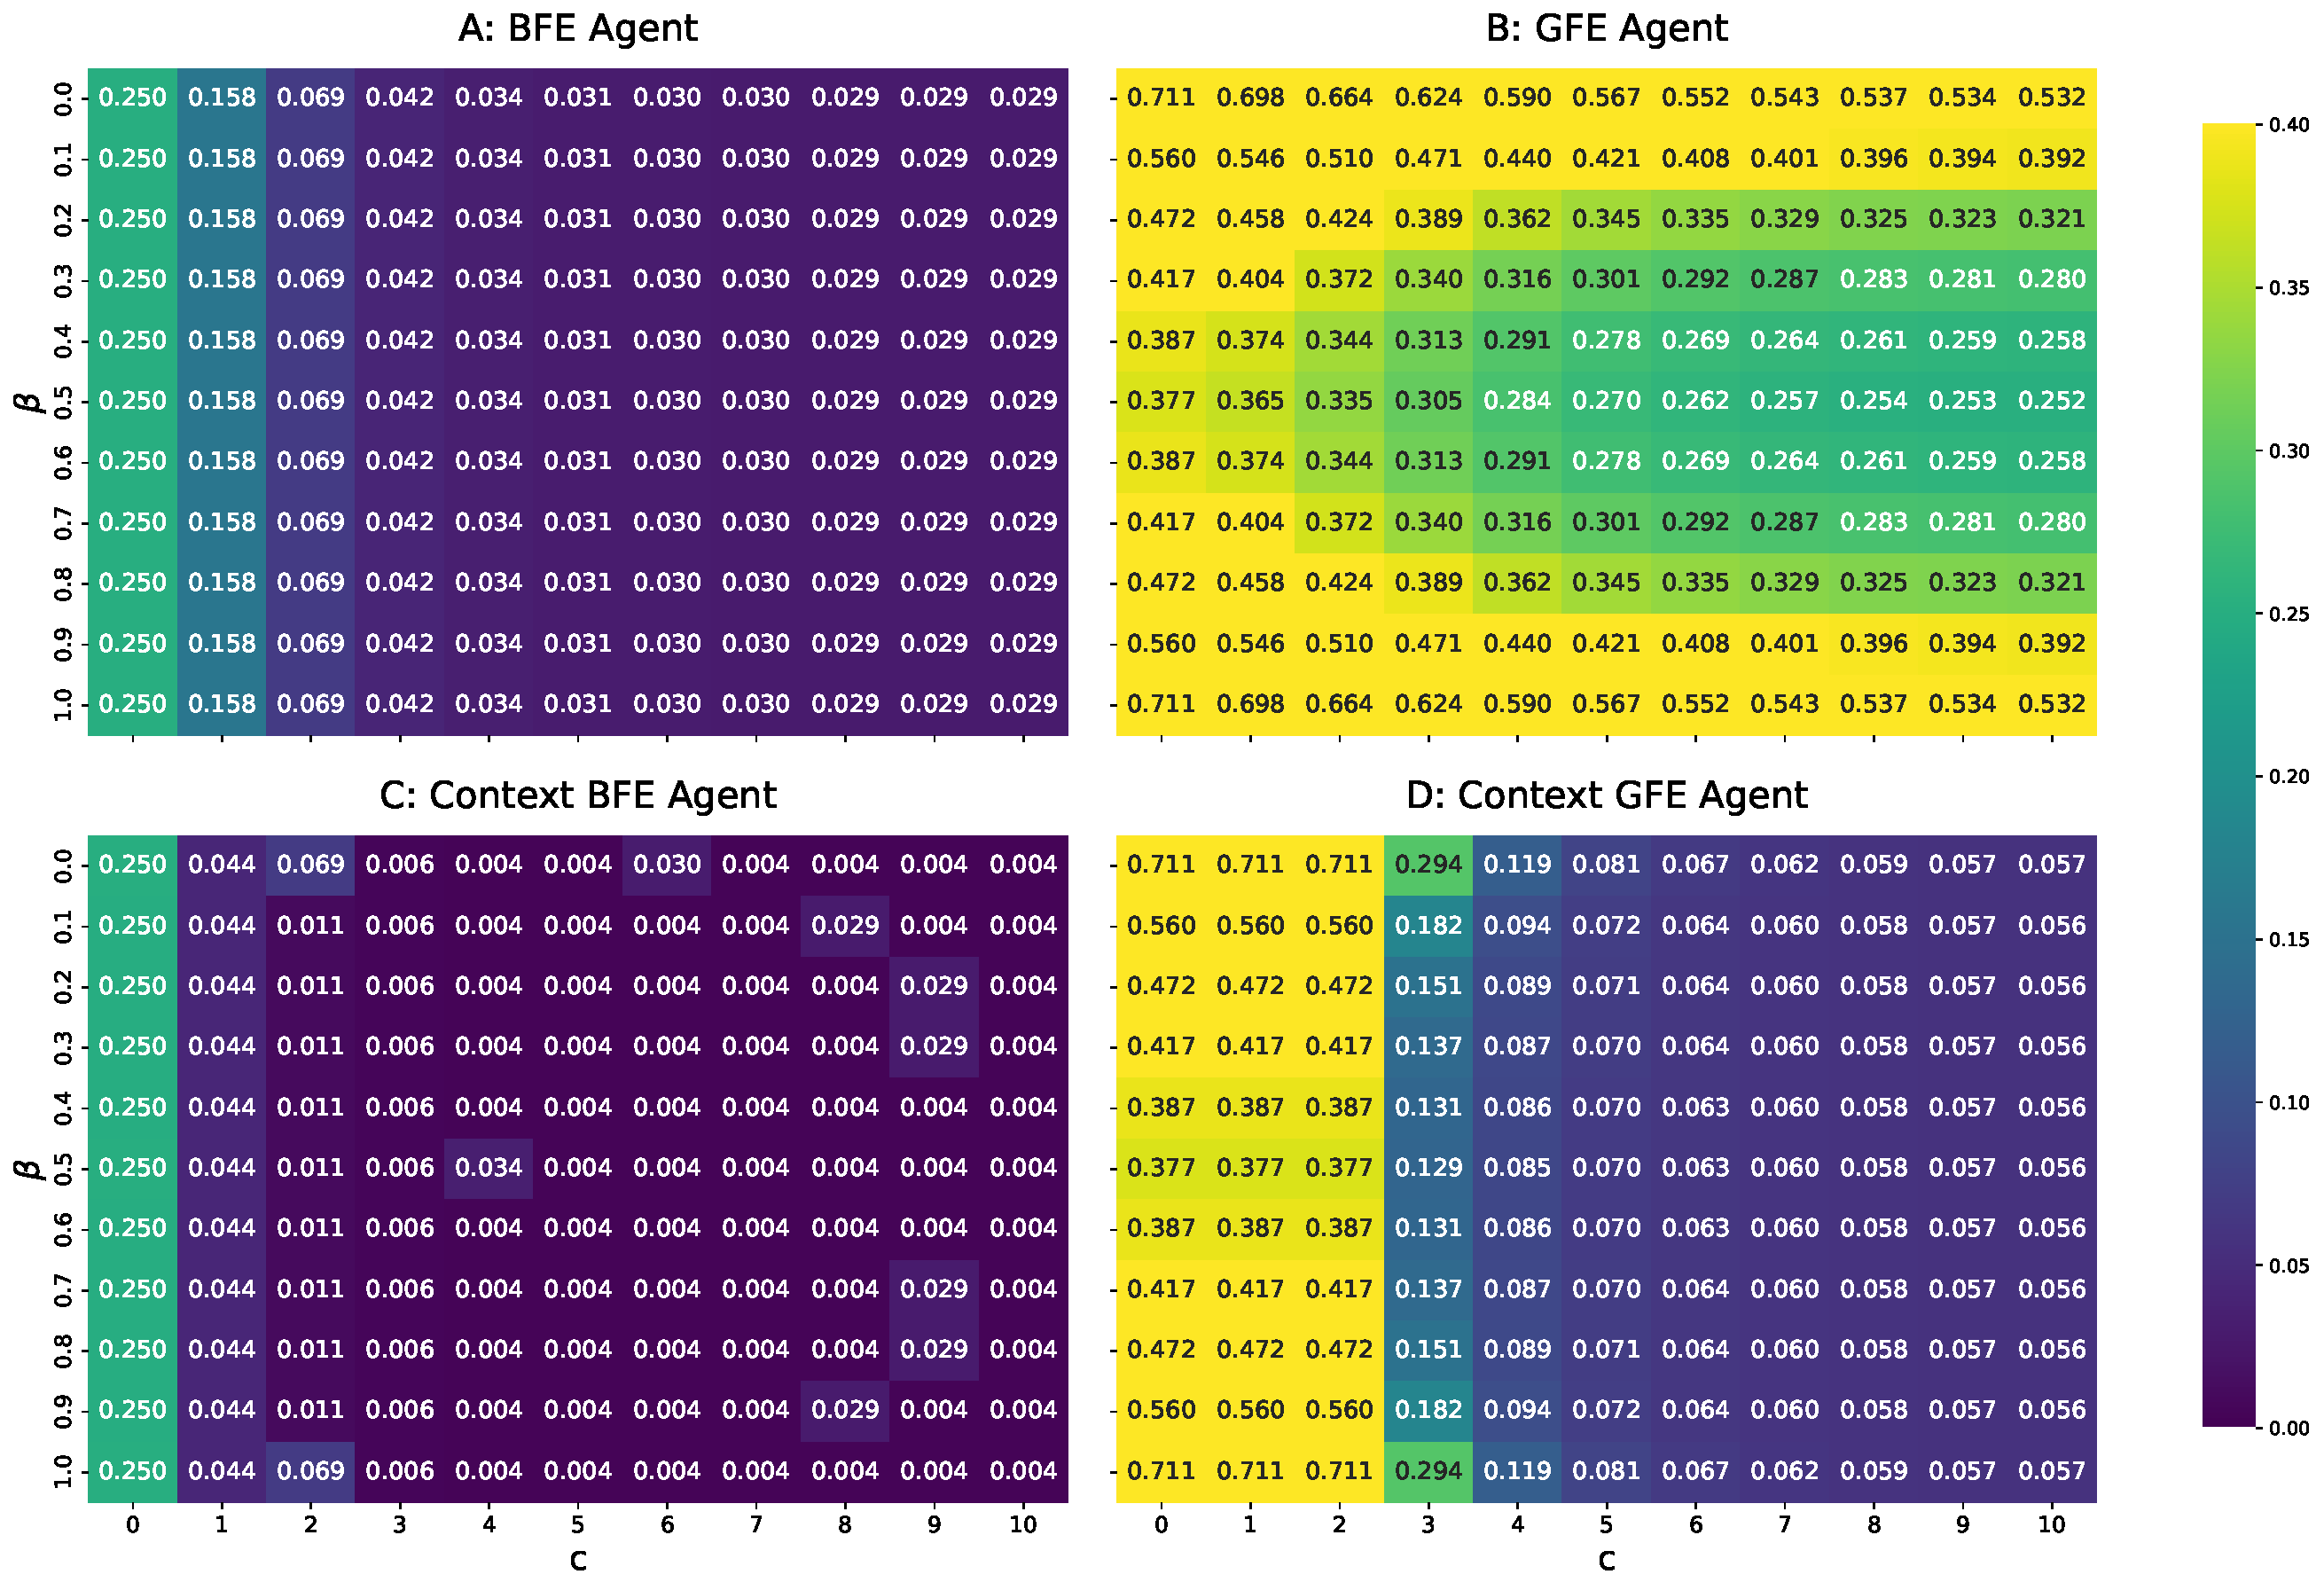
\includegraphics[width=\textwidth]{figures/simulation_1_cue.pdf}
    \caption{Inferred probabilities of executing an action in timestep \(t=0\) that moves the agent to the cue for the four agents (BFE, GFE, Context-BFE, and Context-GFE) with differing \(\alpha\)- and \(c\) values.}
    \label{fig:19}
\end{figure}

\subsubsection{Desire for observing the Reward}

All agents know the reward is located in one of the two arms in the T-Maze but certaintly not at the two remaining locations (start and cue). When the agent has a stronger preference for the reward (higher \(c\) value) then it is also more likely to directly move to one of two arms and effectively gambles for the reward (there is a \(50\,\%\) chance of observing the reward). In return the probabilities of performing an alternative action (e.g., "move to cue", or "move (stay) at start") become smaller. This consequence is evident in each agent type, where the probabilities of moving to the cue become smaller for larger \(c\) values.

\subsubsection{Desire for reducing Uncertainty}

The drive for reducing uncertainty about hidden states (including context states) is only evident in the curious agents. In the following, I explain the curiousity mechanism and how it relates to the results of the agents. High uncertainty levels of hidden states in the generative model relates to the agent's assumption that some hidden causes of observations in the environment are not clear, meaning the agent assigns similar (highly entropic) probabilities to the different possible causes. In this simulation, the hidden causes of observations consist of the four T-Maze fields (left arm, right arm, start, and cue) and the two T-Maze types (type A, and type B). Regarding the fields, they are immediately disclosed at each observation, e.g., when the agent is at the start it immediately knows (through the observation) that it is at the start field. In the case of the T-Maze types observations do not regularly reveal the type of the maze. This situation is mirrored in the agents' belief distributions about hidden states where the states concerning the T-Maze type initially are maximally uncertain, i.e., both possibilities (type A and type B) have equal (highly entropic) probabilities \(p=0.5\). The curiousity mechanism then aims at reducing this uncertainty (entropy). This is achieved by selecting actions that are expected to lead to observations that are informative about this hidden state. This requires further clarification: Observations can only be informative about hidden states when the agent has a model of the relation between that hidden state and possible observations, i.e, this relation must not be random. This circumstance can directly be exploited by the curious agent by moving to the cue location. There it receives an observation for which the agent possesses a deterministic model how this observation relates to the T-Maze type (one possible observation leads to \(p=1.0\) for type A and the other possible observation leads to \(p=1.0\) for type B). Besides directly moving to the cue location, there is a second option. The agent could also directly move to one of the two arms and thus observes the reward or no reward. This observation is also related to the T-Maze type but not deterministically but through the parameter \(\alpha\). This second option is only useful when \(\alpha \neq 0.5\), i.e, when there is a non-random relation between the observation and the T-Maze type. Moreover, more deterministic values like \(\alpha=0.0\) or \(\alpha=1.0\) makes this observation (reward) more useful, where it can then infer that the maze has type A in the former case and type B for the latter. In this situation, receiving no reward in an arm is also informative because the agent can then infer it is interacting with the opposite maze type. This circumstance becomes evident in the results of both curious agents. Both agents are driven by their curiousity and can only satisfy this "desire" by either going to the cue or moving to one of the arms--but only in the case when it knows what an observation at an arm means in relation to the hidden T-Maze type, i.e, when \(\alpha \neq 0.5\). In the most ambiguous case \(\alpha=0.5\), moving to an arm cannot satisfy the curiousity drive, i.e, it does not reduce uncertainty about the T-Maze type and thus the agent is then increasingly driven to reduce this uncertainty using the other option it still has: It instead moves to the cue. This trend is visible in the results of both curious agents where they initially move to the cue with highest probabilities (\(p=0.380\)) for \(\alpha\) values near \(0.5\). There is an additional aspect to consider: Though the agent has two options to satisfy its curiousity drive, one of them is potentially risky. When opting for moving to an arm to find out about the T-Maze type, it potentially misses out on the reward, which it strongly dislikes. In this way, curious agents balance the value of information with the value of receiving preferred observations, i.e., both motives have the same "currency".


\section{Experiment 2: Exploiting Information}

In this section I analyze the results of \cref{fig:20}. Again, the following behavioral analysis can be divided into two parts that first relate to all agents' drive to receive the reward, and second relate to the curious agents' drive to also seek information in the environment.
The values in the heatmaps' cells (\cref{fig:20}) give the inferred probabilities of moving to the arm in the T-Maze that is hinted by the cue to contain the reward (via the T-Maze type and parameter \(\alpha\). Again, the probabilities do not represent empirical measurements but beliefs of the agent that it will execute the action that moves it to the arm that should contain the reward according to the cue.

\begin{figure}[htb]
    \centering
    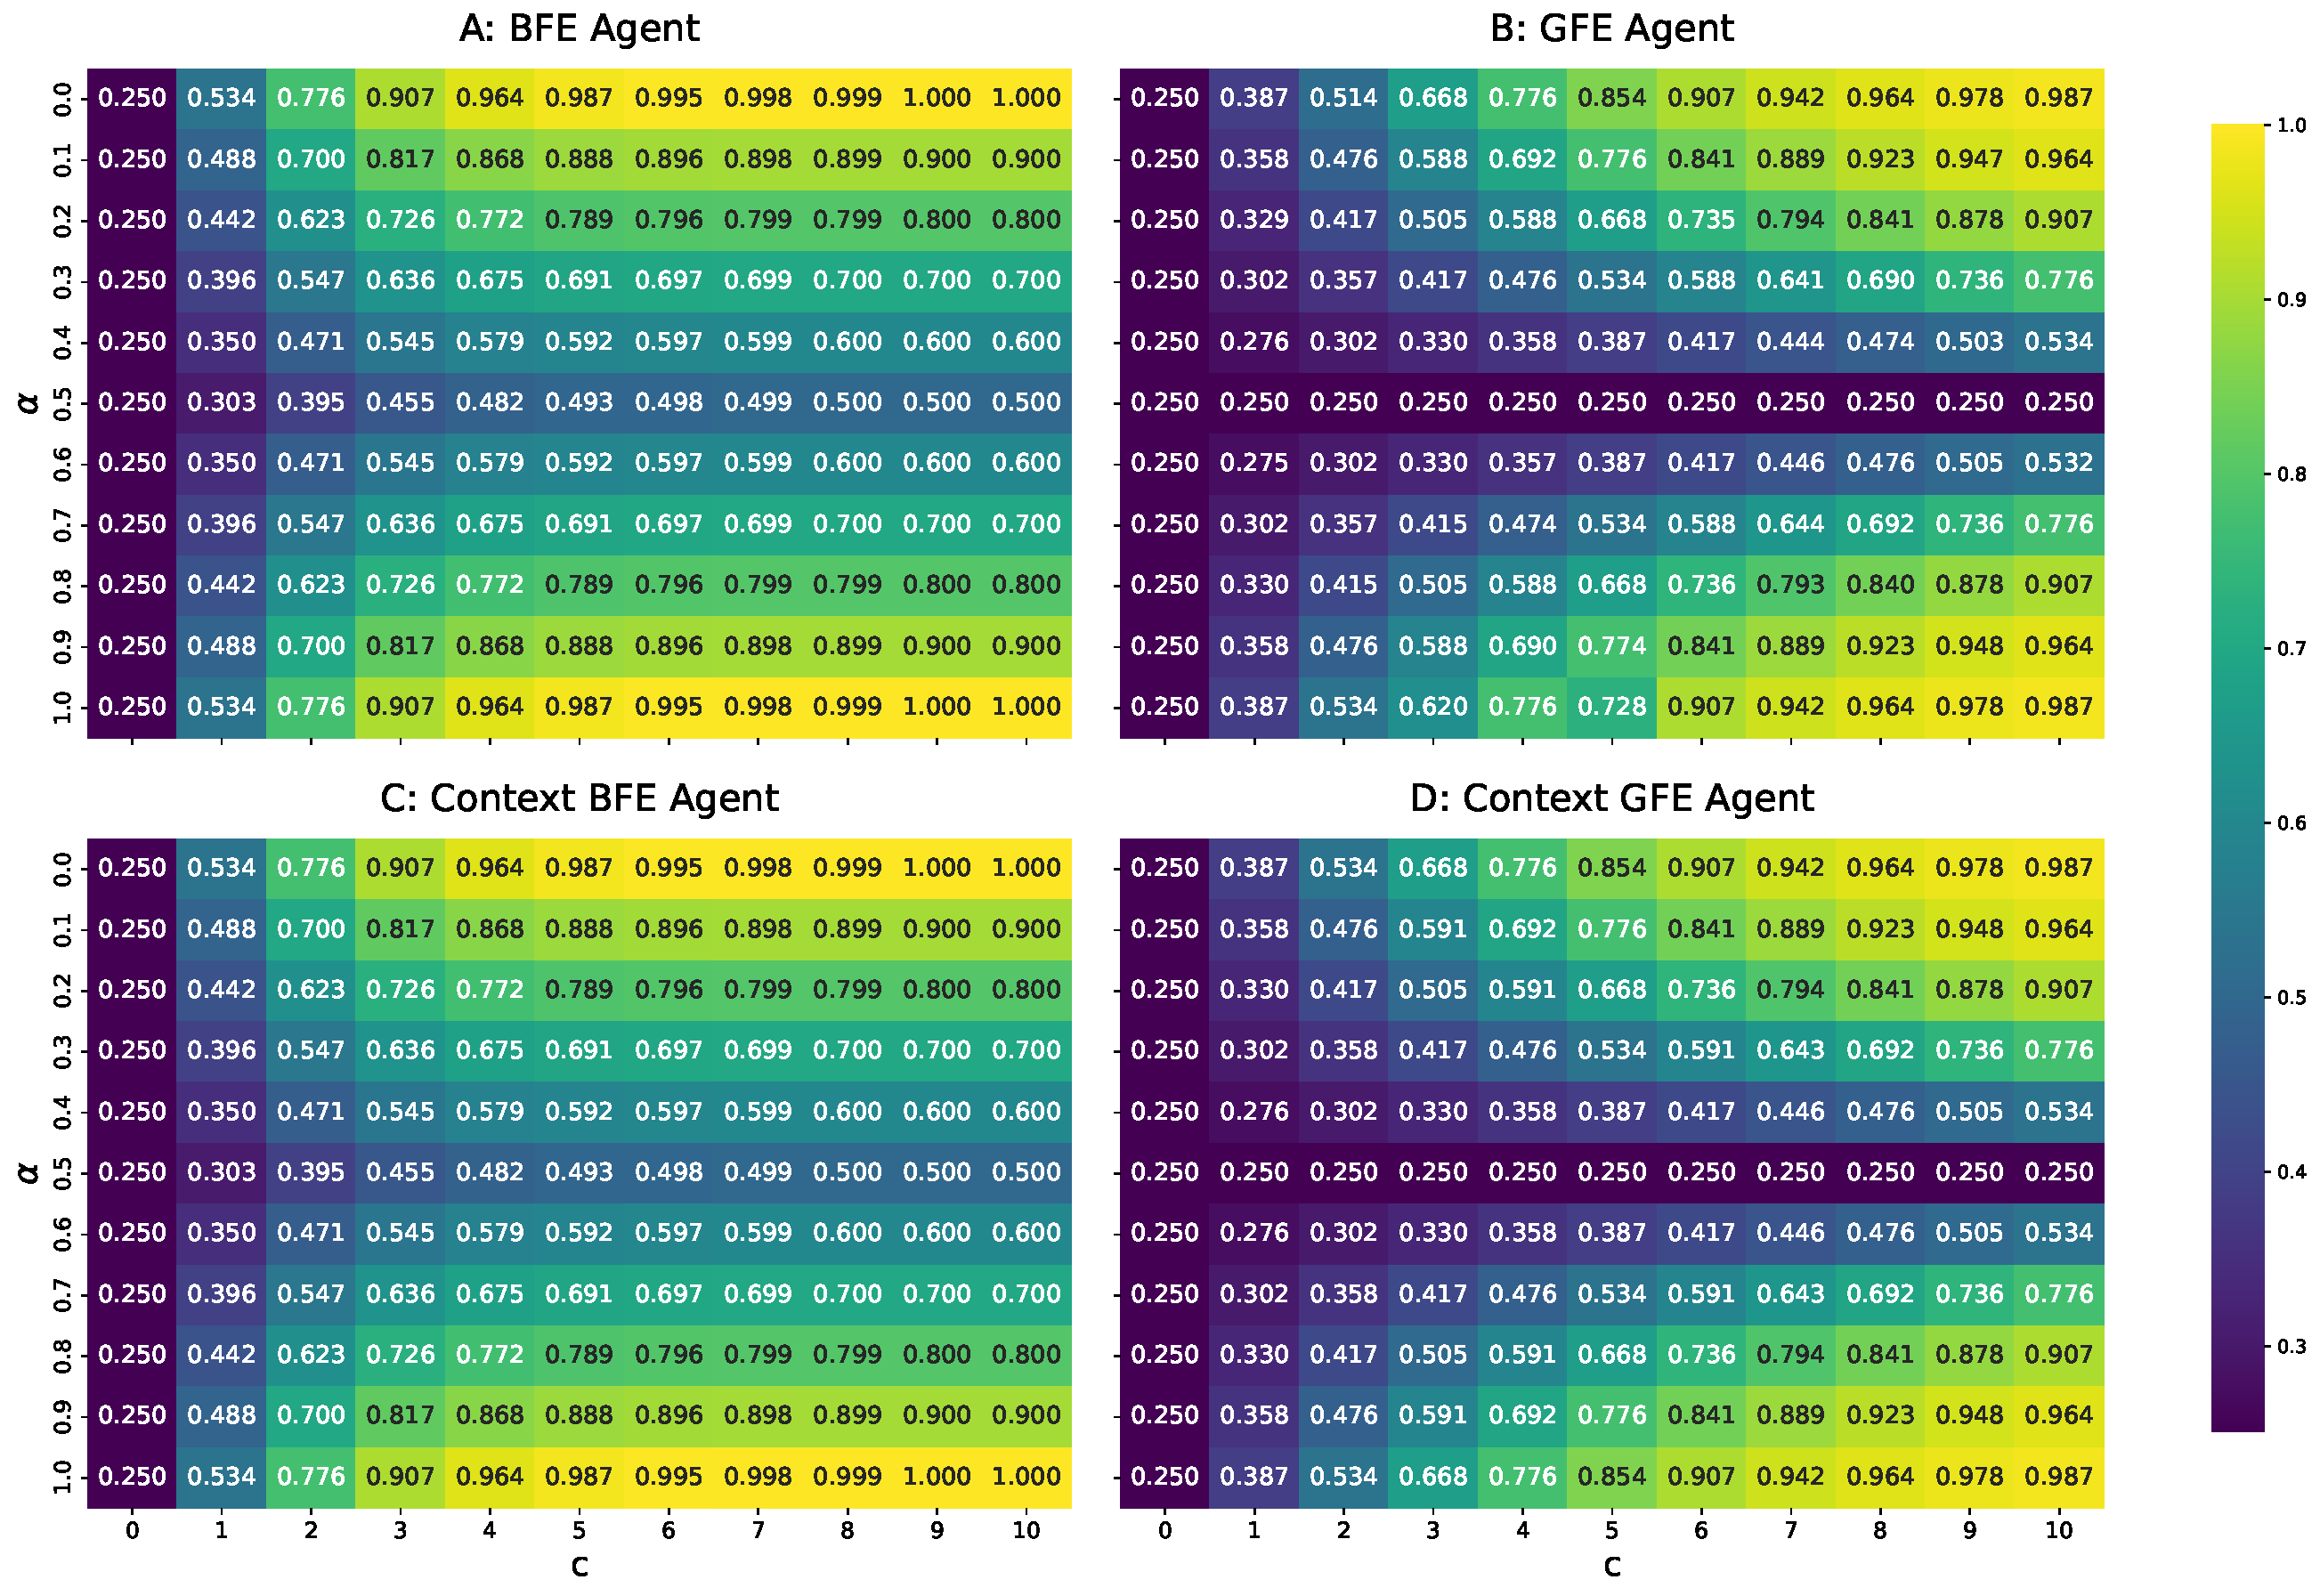
\includegraphics[width=\textwidth]{figures/simulation_2.pdf}
    \caption{Inferred probabilities of moving to the arm in the T-Maze that is hinted by the cue to contain the reward for the four agents (BFE, GFE, Context-BFE, and Context-GFE) with differing \(\alpha\)- and \(c\) values.}
    \label{fig:20}
\end{figure}

\subsubsection{Moving to the cued Reward Field}

All four agents show similar characteristics of moving to the arm field that is suggested by the cue. Specifically, the cue reveals the type of the T-Maze (type A or type B) and the agents can relate this information to the specific arm that is expected to contain the reward via the parameter \(\alpha\). Extreme \(\alpha\) values allow for a more certain prediction of the cue-containing arm field. This situation is evident in all four agents. The probabilities of moving to the arm that is suggested by the cue increase with more certain (extreme) \(\alpha\) values, i.e., the agents know there is a strong correlation between the T-Maze type and the location of the reward (left arm or right arm) and exploit this knowledge to find the reward.

Similarly, the \(c\) values describe the agents' preferences of observing the reward, where higher values lead to stronger preferences. This circumstance is visible in the results of all four agents where they all are more likely to move to the cued reward location with increasing \(c\) values, i.e, the more they "want" to receive the reward the more likely they exploit the information from the cue.

\subsubsection{Curious Agents still seek Information}

Both curious agents have similar results compared to the non-curious agents with subtle differences that seem to relate to their intrinsic drive to continue seeking information in the environment (even after receiving the cue). The curious agents yield lower probabilities of moving to the cued location for most \(\alpha\)- and \(c\) values, i.e., in these cases the curious agents assign more probability mass to other actions which indicates that these still reveal information that the agents seek. The few configurations of \(\alpha\)- and \(c\) values that have higher probabilities than the non-curious agents hint at the opposite: There the curious agents seem to assume information at these cued fields that can be exploited. These findings require further investigation.


\section{Experiment 3: Long-Term Success}


In this section I give the results of \cref{fig:21}. As for previous simulations the results show a behavioral divide between non-curious and curious agents. These are detailed in the following.
The values in the heatmaps' cells give the ratios of receiving the reward in timestep \(t=1\) or \(t=2\) over \(1000\) trials.

\begin{figure}[htbp]
    \centering
    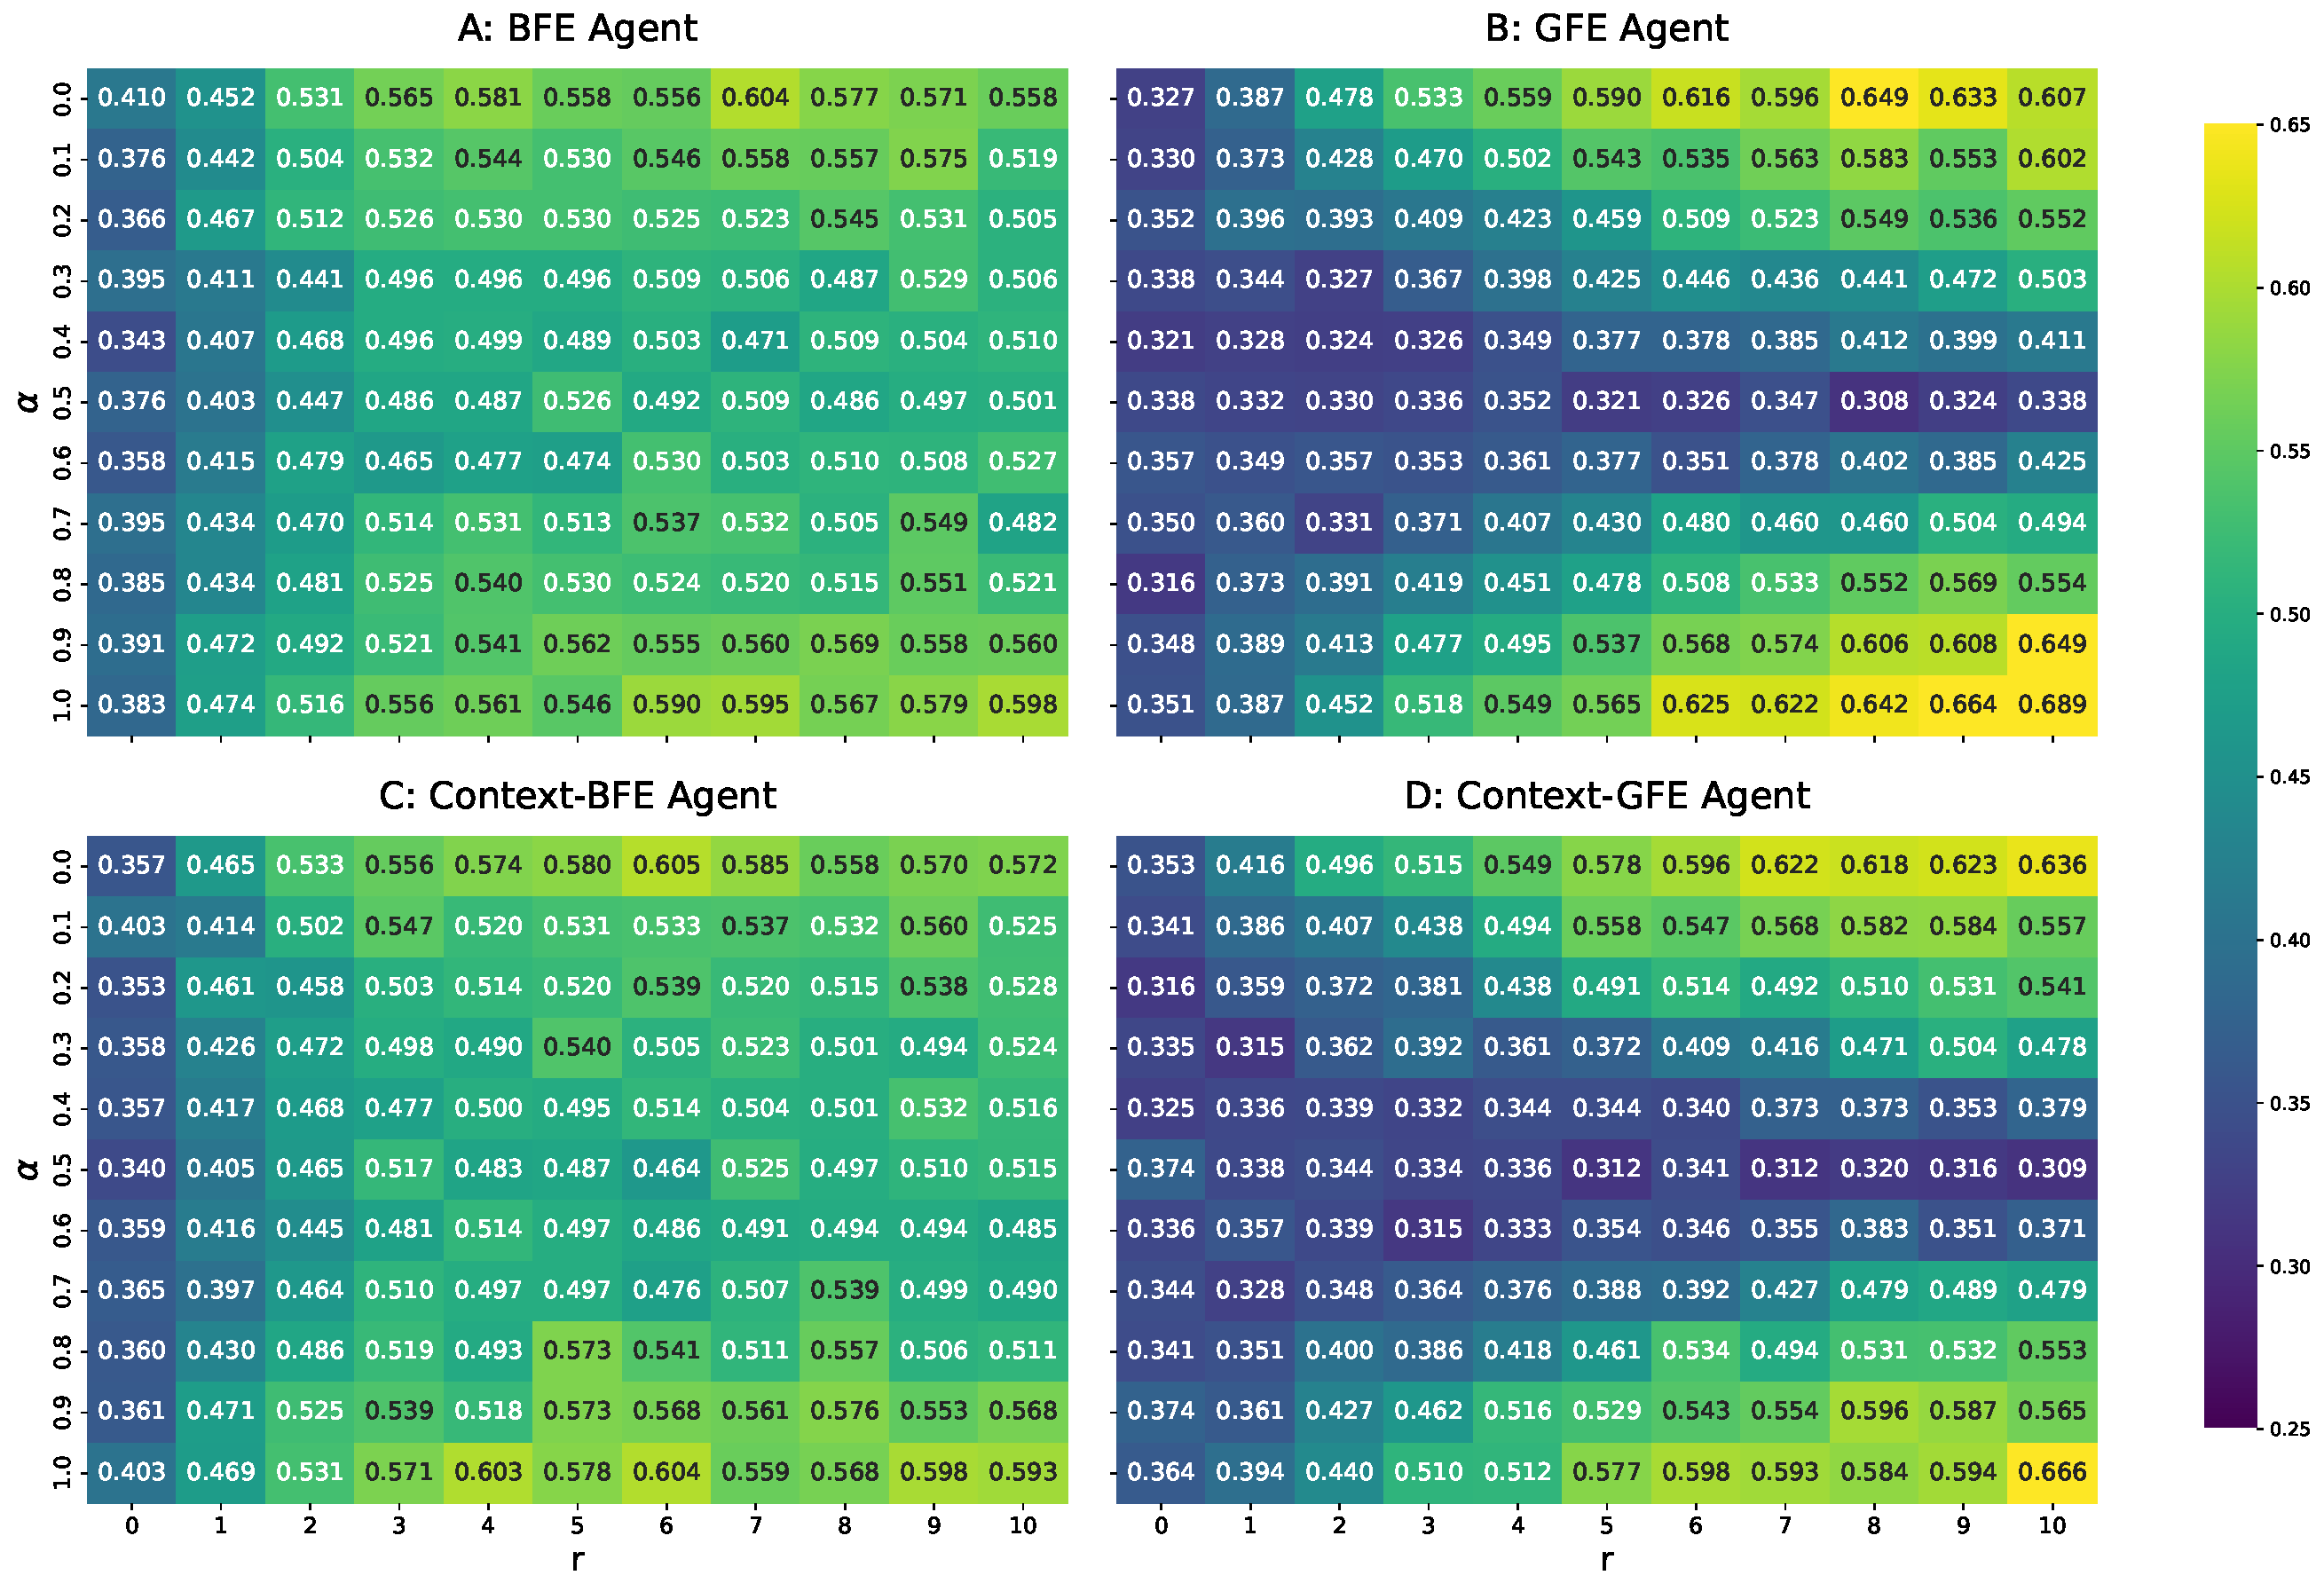
\includegraphics[width=\textwidth]{figures/simulation_3.pdf}
    \caption{Ratios of receiving the reward in timestep \(t=1\) or \(t=2\) over \(1000\) trials for the four agents (BFE, GFE, Context-BFE, and Context-GFE) with differing \(\alpha\)- and \(c\) values.}
    \label{fig:21}
\end{figure}

\subsubsection{Success Factors}

First, I consider the trends that are evident in all four agents. Generally, higher \(c\) values and more extreme \(\alpha\) values lead to higher success rates of receiving the reward in a trial. This is plausible since higher \(c\) values increase the agents' drive of pursuing the reward and more extreme \(\alpha\) values render the cue more useful for moving to the correct arm that contains the reward.

\subsubsection{Curious Agents}

The curious agents appear to have lower success rates for many combinations of \(\alpha\)- and \(c\) values. In these cases their drive of curiousity seem to lead them to alternative behavioral pathways such that they miss out on the reward more regularly.
This situation changes for extreme \(\alpha\)- and high \(c\) values. For these configurations the curious agents receive the reward more regularly than the non-curious agents. In these rare cases, the curious agents "hit" the right balance of going to the cue in the first timestep and being able to use this information in the second step.

\chapter{Discussion}

In this thesis I first reproduced two behavioral models (BFE- and GFE agent) from ... that are capable of perception, planning, and action. Both are based on free energy functionals from which message passing schemes are derived. Message passing enables them with inference, which in turn gives rise to their full behavioral repetoire. The GFE agent is based on the BFE agent but additionally entails a mechanism that reduces the uncertainty of its hidden state (part of its generative model) by seeking information in the environment via actions, i.e., it is curious.
In a second step, I expanded the free energy functional of the BFE agent to introduce a hidden context state in the generative model, which gave rise to the Context-BFE agent. The corresponding message passing algorithm was derived from this expanded free energy.
In a third step, I took the integration of the information seeking mechanism in the GFE agent as an example to introduce this mechanism to the Context-BFE agent for the context state, i.e., the mechanism leads to information seeking that reduces uncertainty of the hidden context state. This integration finally led to the Context-GFE agent. From its customized free energy functional I derived the corresponding message passing algorithm.
I tested all four agents in the simulated T-Maze environment which is frequently used to reveal information seeking behavior. There I showed that the newly developed Context-GFE agent shows similar behavior to the GFE agent, which strongly suggests that the integration of the information seeking mechanism in the Context-GFE agent was successful, i.e., it is curious like the GFE agent and is driven to reduce uncertainty over its hidden (context) state. As a baseline, I also gave the results for both non-curious agents (BFE- and Context-BFE), which both show similar (non-information seeking) behavior.
Beyond that, I generally addressed the kind of behavior that results from the information seeking mechanism in both curious agents (not uniquely tied to the newly developed Context-GFE agent).

\section{Interpretation}



-alternative meaning of success
-attention parameter
-beta sweep
-alpha sweep for comparability with de Vries papers

\section{Limitations}

\subsubsection{Compromises of the Mean-Field Approximation in the Context-GFE agent}

While the results of both curious agents are qualitatively similar, they are not equal, meaning that although the Context-GFE agent also performs information seeking like the GFE agent, there are subtle differences that are addressed in the following. The Context-GFE agent shows a more abrupt transition of probabilities from smaller \(c\) values and \(\alpha\) values near \(0.5\) to larger \(c\) values and more extreme \(\alpha\) values. This phenomenon is most likely a consequence of a mean-field approximation that was necessary to develop the Context-GFE agent. Specifically, while the GFE agent models the T-Maze type as part of its hidden state, the Context-GFE agent instead models it via its context state. The differences between the two approaches are as follows. The hidden state is modeled individually for each timestep in the trial (simulation) while there is only a single context state that persists for the whole trial (see ...). Furthermore, all three observations are related to this single context state in the agent's generative model, i.e, in the factor graph representation there are edges between all observation states and the context state. This leads to cycles in the factor graph which can lead to inference algorithms that do no converge to a stable solution in the case when the statistical dependencies between variables at each node are respected by the local belief distributions, i.e, when we assume the Bethe free energy at each local node. As a remedy, it is sufficient to break these local statistical dependencies at single nodes to remove the cycles. This was done between the observation states and the context state and leads to mean-field approximations at these local nodes. As a result, the inference process leads to stable solutions but has the problem of disrespecting uncertainties in the generative model related to context- and observation states. As a consequence, inference can yield results that are overconfident and thus are not as nuanced as without using the mean-field approximation. This circumstance becomes evident in the results of both curious agents where the GFE agent does not rely on the mean-field approximation between its observation states and hidden states (it does not have a context state and instead models the T-Maze type via the hidden states) and thus achieves a nuanced behavioral shift with varying \(\alpha\)- and \(c\) values. In contrast, the Context-GFE agent relies on the mean-field approximation at the prescribed locations in its generative model and becomes overly confident more quickly with varying parameter combinations (\(\alpha\) and \(c\)) which leads to the visible abrupt change of probabilities for larger \(c\) values and extreme \(\alpha\) values.

\subsubsection{Alternative Meaning of Success}

This situation should not be mistaken to be a weakness of curious agents, instead it shows their inclination of not only preferring predicted observations (like non-curious agents do) but also value hidden environmental causes that are less ambiguous, i.e, they seek to reduce uncertainty about their model of these causes, which are the hidden states. This mechanism may allow them to reduce their variational free energy more reliably in the long term and thus better secure their existence in evolutionary terms (according to the Free Energy Principle). In this way, the term "Long-Term Success" might not only be understood as the rates of receiving the reward but additionally refers to the agent's ability to minimize its variational free energy which necessitates the curiousity mechanism.


\section{Outlook}
\chapter{Conclusion}
\label{chap:5}

Humans' capabilities of seeking information in the environment to reduce uncertainties regarding abstract context states are evident. Towards understanding the underlying mechanisms I developed a computational model of this kind of behavior. The model is based on the active inference framework, that allows for the specification of agents, i.e., models of behavior, with a curiousity drive. The resulting agent (Context-GFE) is capable of reducing uncertainty with respect to an abstract context state in its generative model by planning into the future and acting purposefully to receive insightful observations. I validated this behavior during simulated experiments in the T-maze environment.

I hope this contribution makes a step forward at establishing the active inference framework as a tool set for developing testable hypotheses for brain functions, mental illnesses, and furthermore for the creation of artifical agents.
\printbibliography
\begin{appendices}

    \chapter{Equality Node Messages}
    \label[appendix]{app:1}

    In this section I present the messages sent by equality nodes. As mentioned before edges in the factor graph are allowed to have a maximum number of connected nodes of two. This is a technical problem because there are variables (edges) that occur in more than two factor function (nodes). As a remedy factor graphs support equality nodes that artificially duplicate the variables and enforce an equality relation between the duplicated variables. This relation is implemented in the factor function of these nodes as a product of Kronecker (or Dirac) delta functions. As an example consider the the factor graph in \cref{fig:39} where we are interested in \(\textcolor{accorange}{\bm{\overleftarrow{\mu}(}s\bm{)}}\), \(\textcolor{accorange}{\bm{\overrightarrow{\mu}(}s^{\scriptscriptstyle I}\bm{)}}\), and \(\textcolor{accorange}{\bm{{\downarrow}{\mu}(}s^{\scriptscriptstyle II}\bm{)}}\).
    \begin{figure}[htbp]
        \centering

        \begin{tikzpicture}[
                factor/.style={draw=black, thick, rectangle, minimum size=0.8cm,
                        font=\normalsize},
                eqfactor/.style={draw=black, thick, rectangle, minimum size=0.5cm, font=\normalsize},
                edge/.style={thick},
                varlabel/.style={font=\normalsize}
            ]

            % Knoten
            \node[eqfactor, label={[varlabel, yshift=0.1cm, scale=0.9]above:$q_a(s,s^{\scriptscriptstyle I},s^{\scriptscriptstyle II})$}] (b) {$=$};

            % Kanten
            \draw[edge] ([xshift=-3cm]b.west) -- (b.west) node[midway, above, varlabel, scale=0.9] {$q_i(s)$} node[near start, below, varlabel, scale=0.9] {$\textcolor{accorange}{\bm{\overleftarrow{\mu}(}s\bm{)}}$} node[near end, below, varlabel, scale=0.9] {$\textcolor{black}{\bm{\overrightarrow{\mu}(}s\bm{)}}$};
            \draw[edge] (b.south) -- ([yshift=-2.5cm]b.south) node[midway, left, varlabel, scale=0.9] {$q_k(s^{\scriptscriptstyle II})$} node[pos=0.75, right, varlabel, scale=0.9] {$\textcolor{accorange}{\bm{{\downarrow}{\mu}(}s^{\scriptscriptstyle II}\bm{)}}$} node[pos=0.25, right, varlabel, scale=0.9] {$\textcolor{black}{\bm{{\uparrow}{\mu}(}s^{\scriptscriptstyle II}\bm{)}}$};
            \draw[edge] (b.east) -- ([xshift=3cm]b.east) node[midway, above, varlabel, scale=0.9] {$q_j(s^{\scriptscriptstyle I})$} node[near end, below, varlabel, scale=0.9] {$\textcolor{accorange}{\bm{\overrightarrow{\mu}(}s^{\scriptscriptstyle I}\bm{)}}$} node[near start, below, varlabel, scale=0.9] {$\textcolor{black}{\bm{\overleftarrow{\mu}(}s^{\scriptscriptstyle I}\bm{)}}$};

        \end{tikzpicture}

        \caption{Example FFG with messages sent by the equality node (\(\textcolor{accorange}{\bm{\overleftarrow{\mu}(}s\bm{)}}\), \(\textcolor{accorange}{\bm{\overrightarrow{\mu}(}s^{\scriptscriptstyle I}\bm{)}}\), and \(\textcolor{accorange}{\bm{{\downarrow}{\mu}(}s^{\scriptscriptstyle II}\bm{)}}\)).}
        \label{fig:39}
    \end{figure}
    The factor function of the equality node is given by
    \begin{equation}
        f_a(s,s^{\scriptscriptstyle I},s^{\scriptscriptstyle II}) = \delta_{s,s^{\scriptscriptstyle I}} \delta_{s,s^{\scriptscriptstyle II}}.
    \end{equation}
    This function is a discrete probability distribution that has probability 1 only if the values of all variables are equal. In other cases it is 0.
    Building on this the Lagrangian (without normalization constraints) of the factor graph is
    \begin{equation}
        \begin{split}
            L = & \sum_{s,s^{\scriptscriptstyle I},s^{\scriptscriptstyle II}} q_a(s,s^{\scriptscriptstyle I},s^{\scriptscriptstyle II}) \log \frac{q_a(s,s^{\scriptscriptstyle I},s^{\scriptscriptstyle II})}{\delta_{s,s^{\scriptscriptstyle I}} \delta_{s,s^{\scriptscriptstyle II}}} + \sum_s \lambda_{ia}(s) (q_i(s) - \sum_{s^{\scriptscriptstyle I},s^{\scriptscriptstyle II}} q_a(s,s^{\scriptscriptstyle I},s^{\scriptscriptstyle II})) \\
                & + \sum_{s^{\scriptscriptstyle I}} \lambda_{ja}(s^{\scriptscriptstyle I}) (q_j(s^{\scriptscriptstyle I}) - \sum_{s,s^{\scriptscriptstyle II}} q_a(s,s^{\scriptscriptstyle I},s^{\scriptscriptstyle II})) + \sum_{s^{\scriptscriptstyle II}} \lambda_{ka}(s^{\scriptscriptstyle II}) (q_k(s^{\scriptscriptstyle II}) - \sum_{s,s^{\scriptscriptstyle I}} q_a(s,s^{\scriptscriptstyle I},s^{\scriptscriptstyle II}))
        \end{split}
    \end{equation}
    Differentiating \(L\) with respect to \(q_a\) then yields:
    \begin{alignat}{3}
         & \frac{\delta L}{\delta q_a(s,s^{\scriptscriptstyle I},s^{\scriptscriptstyle II})} &  & = \log q_a(s,s^{\scriptscriptstyle I},s^{\scriptscriptstyle II}) + 1 - \log (\delta_{s,s^{\scriptscriptstyle I}} \delta_{s,s^{\scriptscriptstyle II}}) - \lambda_{ia}(s) - \lambda_{ja}(s^{\scriptscriptstyle I}) - \lambda_{ka}(s^{\scriptscriptstyle II})               & \; \overset{!}{=} 0 \\
         &                                                                                   &  & \Rightarrow q_a^*(s,s^{\scriptscriptstyle I},s^{\scriptscriptstyle II}) \propto \delta_{s,s^{\scriptscriptstyle I}} \delta_{s,s^{\scriptscriptstyle II}} \exp(\lambda_{ia}(s)) \exp(\lambda_{ja}(s^{\scriptscriptstyle I})) \exp(\lambda_{ka}(s^{\scriptscriptstyle II}))
    \end{alignat}
    Finally, we use the result of \cref{sec:1} for the local stationary points of \(q_i(s)\), \(q_j(s^{\scriptscriptstyle I})\), and \(q_k(s^{\scriptscriptstyle II})\) and use the marginalization constraints \(q_i(s) \overset{!}{=} \sum_{s^{\scriptscriptstyle I},s^{\scriptscriptstyle II}} q_a(s,s^{\scriptscriptstyle I},s^{\scriptscriptstyle II})\), \(q_j(s^{\scriptscriptstyle I}) \overset{!}{=} \sum_{s,s^{\scriptscriptstyle II}} q_a(s,s^{\scriptscriptstyle I},s^{\scriptscriptstyle II})\), and \(q_k(s^{\scriptscriptstyle II}) \overset{!}{=} \sum_{s,s^{\scriptscriptstyle I}} q_a(s,s^{\scriptscriptstyle I},s^{\scriptscriptstyle II})\) to determine the messages \(\textcolor{accorange}{\bm{\overleftarrow{\mu}(}s\bm{)}}\), \(\textcolor{accorange}{\bm{\overrightarrow{\mu}(}s^{\scriptscriptstyle I}\bm{)}}\), and \(\textcolor{accorange}{\bm{{\downarrow}{\mu}(}s^{\scriptscriptstyle II}\bm{)}}\) sent by the equality node:
    \begin{alignat}{2}
         & q_i^*(s)                                                                                                                                                                                                                                                                                                                                                                  &  & \overset{!}{=} \sum_{s^{\scriptscriptstyle I},s^{\scriptscriptstyle II}} q_a^*(s,s^{\scriptscriptstyle I},s^{\scriptscriptstyle II})                                                                                                                        \\
         & \exp(\lambda_{ia}(s)) \exp(\lambda_{i\bullet}(s))                                                                                                                                                                                                                                                                                                                               &  & \propto \sum_{s^{\scriptscriptstyle I},s^{\scriptscriptstyle II}} \delta_{s,s^{\scriptscriptstyle I}} \delta_{s,s^{\scriptscriptstyle II}} \exp(\lambda_{ia}(s)) \exp(\lambda_{ja}(s^{\scriptscriptstyle I})) \exp(\lambda_{ka}(s^{\scriptscriptstyle II})) \\
         & \mathrlap{\Rightarrow \exp(\lambda_{i\bullet}(s))              \propto \sum_{s^{\scriptscriptstyle I},s^{\scriptscriptstyle II}} \delta_{s,s^{\scriptscriptstyle I}} \delta_{s,s^{\scriptscriptstyle II}} \exp(\lambda_{ja}(s^{\scriptscriptstyle I})) \exp(\lambda_{ka}(s^{\scriptscriptstyle II}))}                                                                                                                                                                                                                                                                                                                                            \\
         & \mathrlap{\Rightarrow \textcolor{accorange}{\bm{\overleftarrow{\mu}(}s\bm{)}} \propto \sum_{s^{\scriptscriptstyle I},s^{\scriptscriptstyle II}} \delta_{s,s^{\scriptscriptstyle I}} \delta_{s,s^{\scriptscriptstyle II}} \textcolor{black}{\bm{\overleftarrow{\mu}(}s^{\scriptscriptstyle I}\bm{)}} \textcolor{black}{\bm{{\uparrow}{\mu}(}s^{\scriptscriptstyle II}\bm{)}}}                                                                                                                                                                                                                                                                 \label{eq:21} \\
         & \mathrlap{\left(\Rightarrow \textcolor{accorange}{\bm{\overleftarrow{\mu}(}s\bm{)}} \propto \textcolor{black}{\bm{\overleftarrow{\mu}(}s\bm{)}} \textcolor{black}{\bm{{\uparrow}{\mu}(}s\bm{)}}\right)} \label{eq:22}
    \end{alignat}
    The "\(\bullet\)" signs in the lambdas indicate the other nodes (not shown in \cref{fig:39}) the respective edge is connected to. The terms that contain these lambdas (i.e., \(\exp \left( \lambda_{i\bullet}(s) \right)\)) are the outgoing messages to these other nodes.
    Analogously, it follows:
    \begin{alignat}{2}
         & \Rightarrow \textcolor{accorange}{\bm{\overrightarrow{\mu}(}s^{\scriptscriptstyle I}\bm{)}} \propto \sum_{s^{\scriptscriptstyle I},s^{\scriptscriptstyle II}} \delta_{s,s^{\scriptscriptstyle I}} \delta_{s,s^{\scriptscriptstyle II}} \textcolor{black}{\bm{\overrightarrow{\mu}(}s\bm{)}} \textcolor{black}{\bm{{\uparrow}{\mu}(}s^{\scriptscriptstyle II}\bm{)}}   \\
         & \Rightarrow \textcolor{accorange}{\bm{{\downarrow}{\mu}(}s^{\scriptscriptstyle II}\bm{)}} \propto \sum_{s^{\scriptscriptstyle I},s^{\scriptscriptstyle II}} \delta_{s,s^{\scriptscriptstyle I}} \delta_{s,s^{\scriptscriptstyle II}} \textcolor{black}{\bm{\overrightarrow{\mu}(}s\bm{)}} \textcolor{black}{\bm{\overleftarrow{\mu}(}s^{\scriptscriptstyle I}\bm{)}}.
    \end{alignat}
    This reveals that outgoing messages from equality nodes (e.g., \(\textcolor{accorange}{\bm{\overleftarrow{\mu}(}s\bm{)}}\) in \cref{eq:21}) are the product of incoming messages (\(\textcolor{black}{\bm{\overleftarrow{\mu}(}s^{\scriptscriptstyle I}\bm{)}} \textcolor{black}{\bm{{\uparrow}{\mu}(}s^{\scriptscriptstyle II}\bm{)}}\)) (except from the neighoring node that is the addresse of the message to be sent) where variables of incoming messages get substituted with the variable of the outgoing message as a result of the summation and the two Kronecker deltas. While in principle this substitution leads to \cref{eq:22} I refrain from that further step because the resulting messages (\(\textcolor{black}{\bm{\overleftarrow{\mu}(}s\bm{)}} \textcolor{black}{\bm{{\uparrow}{\mu}(}s\bm{)}}\)) might be misunderstood for the messages that are actually sent on the edge of variable \(s\). Instead they really are the incoming messages from the edges of variables \(s^{\scriptscriptstyle I}\) and \(s^{\scriptscriptstyle II}\) respectively where the variables got substituted with \(s\).

\end{appendices}

\end{document}